% Options for packages loaded elsewhere
\PassOptionsToPackage{unicode}{hyperref}
\PassOptionsToPackage{hyphens}{url}
%
\documentclass[12pt,a4paper]{report}


\usepackage{setspace}
\usepackage{amsmath}
\usepackage{amsfonts}
\usepackage{lmodern}
\usepackage{amssymb}
\usepackage{iftex}
\usepackage{amsfonts}
\usepackage{wrapfig}
\usepackage{pdflscape}
\usepackage{placeins} % provides \FloatBarrier
\usepackage{comment} % for comment environment
\numberwithin{equation}{section}


\ifPDFTeX
  \usepackage[T1]{fontenc}
  \usepackage[utf8]{inputenc}
  \usepackage{textcomp} % provide euro and other symbols
\else % if luatex or xetex
  \usepackage{unicode-math}
  \defaultfontfeatures{Scale=MatchLowercase}
  \defaultfontfeatures[\rmfamily]{Ligatures=TeX,Scale=1}
\fi
% Use upquote if available, for straight quotes in verbatim environments
\IfFileExists{upquote.sty}{\usepackage{upquote}}{}
\IfFileExists{microtype.sty}{% use microtype if available
  \usepackage[]{microtype}
  \UseMicrotypeSet[protrusion]{basicmath} % disable protrusion for tt fonts
}{}
\makeatletter
\@ifundefined{KOMAClassName}{% if non-KOMA class
  \IfFileExists{parskip.sty}{%
    \usepackage{parskip}
  }{% else
    \setlength{\parindent}{0pt}
    \setlength{\parskip}{6pt plus 2pt minus 1pt}}
}{% if KOMA class
  \KOMAoptions{parskip=half}}
\makeatother
\usepackage{xcolor}
\IfFileExists{bookmark.sty}{\usepackage{bookmark}}{\usepackage{hyperref}}
\hypersetup{
  hidelinks,
  pdfcreator={LaTeX via pandoc}}
\urlstyle{same} % disable monospaced font for URLs
\usepackage{longtable,booktabs,array}
\usepackage{calc} % for calculating minipage widths
% Correct order of tables after \paragraph or \subparagraph
\usepackage{etoolbox}
\makeatletter
\patchcmd\longtable{\par}{\if@noskipsec\mbox{}\fi\par}{}{}
\makeatother
% Allow footnotes in longtable head/foot
\IfFileExists{footnotehyper.sty}{\usepackage{footnotehyper}}{\usepackage{footnote}}
\makesavenoteenv{longtable}
\usepackage{graphicx}
\makeatletter
\def\maxwidth{\ifdim\Gin@nat@width>\linewidth\linewidth\else\Gin@nat@width\fi}
\def\maxheight{\ifdim\Gin@nat@height>\textheight\textheight\else\Gin@nat@height\fi}
\makeatother
% Scale images if necessary, so that they will not overflow the page
% margins by default, and it is still possible to overwrite the defaults
% using explicit options in \includegraphics[width, height, ...]{}
\setkeys{Gin}{width=\maxwidth,height=\maxheight,keepaspectratio}
% Set default figure placement to htbp
\makeatletter
\def\fps@figure{htbp}
\makeatother
\usepackage[normalem]{ulem}
% Avoid problems with \sout in headers with hyperref
\pdfstringdefDisableCommands{\renewcommand{\sout}{}}
\setlength{\emergencystretch}{3em} % prevent overfull lines
\providecommand{\tightlist}{%
  \setlength{\itemsep}{0pt}\setlength{\parskip}{0pt}}
\setcounter{secnumdepth}{5}

% Customize chapter headings to remove automatic "Chapter X" prefix
\usepackage{titlesec}
\titleformat{\chapter}[display]
  {\normalfont\huge\bfseries}{}{0pt}{\Huge}
\titlespacing*{\chapter}{0pt}{-30pt}{20pt}

\ifLuaTeX
\usepackage{selnolig}  % disable illegal ligatures
\fi

% Bibliography management with biblatex
\usepackage[backend=biber, style=ieee, sorting=none, citestyle=numeric-comp, defernumbers=true]{biblatex}
\addbibresource{references.bib}
\addbibresource{publications.bib}

% Define category for own publications
\DeclareBibliographyCategory{ownpubs}
\addtocategory{ownpubs}{P1,P2,P3,P4}

% Custom numbering for publications: [P1], [P2], etc.
\DeclareFieldFormat[article,inproceedings,misc]{labelnumber}{\ifcategory{ownpubs}{P#1}{#1}}

% Counter for publications
\newcounter{pubcount}
\defbibenvironment{publist}
  {\list
     {\printtext[labelnumberwidth]{%
        \printfield{prefixnumber}%
        [P\thepubcount]}}
     {\setlength{\labelwidth}{\labelnumberwidth}%
      \setlength{\leftmargin}{\labelwidth}%
      \setlength{\labelsep}{\biblabelsep}%
      \addtolength{\leftmargin}{\labelsep}%
      \setlength{\itemsep}{\bibitemsep}%
      \setlength{\parsep}{\bibparsep}}%
      \renewcommand*{\makelabel}[1]{##1\hss}}
  {\endlist}
  {\stepcounter{pubcount}\item}

\author{}
\date{}

\begin{document}

\onehalfspacing

\begin{titlepage}
\centering
\vspace*{2cm}
{\Large\bfseries FRACTAL BASED FRAMEWORK FOR TIME SERIES VOLATILITY PREDICTION\par}
\vspace{2cm}
{\Large\bfseries Georgy Urumov\par}
\vfill
A thesis submitted in partial fulfilment of the\\
requirements of the University of Westminster\\
for the degree of Doctor of Philosophy\\
\vspace{1.5cm}
October 2025
\end{titlepage}

\clearpage
\pagenumbering{roman}
\setcounter{page}{1}



\emph{\hfill\break
}

\emph{``So limited is our knowledge that we resort, not to science, but
to shamans. We place control of the world's largest economy in the hands
of a few elderly men, the central bankers..''}

\emph{--\/--\/--Benoit Mandlebrot}

\hypertarget{abstract}{%
\chapter*{Abstract}\label{abstract}
\addcontentsline{toc}{chapter}{Abstract}
}

In this thesis, a novel mathematical framework is presented for pricing
financial derivatives and modelling asset behaviour by bringing together
fractional Brownian motion (fBm), fuzzy logic, and jump processes, all
aligned with the no--arbitrage principle. In particular, our mathematical
developments include fBm defined through Mandelbrot--Van Ness kernels,
and advanced mathematical tools such Molchan martingale and BDG
inequalities ensuring rigorous theoretical validity. These different concepts are combined to model uncertainties such as sudden market
shocks and investor sentiment, providing a fresh perspective in
financial mathematics and derivatives pricing. Using fuzzy logic to incorporate subject factors such as market optimism or pessimism,
adjusting volatility dynamically according to the current market
environment. Fractal mathematics with the Hurst exponent close to zero
reflecting rough market conditions and fuzzy set theory are combined
with jumps, representing sudden market changes to capture more realistic
asset price movements. The gap between complex stochastic
equations and solvable differential equations  is bridged using tools like
Feynman--Kac approach and Girsanov transformation. Simulations
illustrating plausible scenarios ranging from pessimistic to optimistic
demonstrate how this model can behave in practice, highlighting
potential advantages over classical models like the Merton jump
diffusion and Black--Scholes. Overall, the proposed model represents an
advancement in mathematical finance by integrating fractional stochastic
processes with fuzzy set theory, thus revealing new perspectives on
derivative pricing and risk--free valuation in uncertain environments.

In financial modelling, traditional approaches often rely on
deterministic frameworks that inadequately capture the inherent
complexities of market dynamics. For example, option pricing models
typically use crisp parameters, yet empirical evidence shows these
variables often exhibit fuzziness and uncertainty. To address these
limitations, this thesis proposes a novel unified framework that
integrates fractional Brownian motion (fBM) and fuzzy processes to model
financial systems characterised by both randomness and fuzziness. By
defining a joint product measure space for H $\in$ (0,1) where H is the
Hurst parameter that characterises the degree of self--similarity and
persistence in fractional Brownian motion, this work provides a
comprehensive framework to account for long--range dependence,
self--similarity, and individual risk preferences in market behaviour.
Building on the Merton jump--diffusion model, we extend the framework to
include fuzzy fractional Brownian motion, fuzzy Poisson processes, and
fuzzy volatility. These innovations enable the modelling of hybrid
systems under uncertain variables, offering practitioners a flexible and
robust tool for understanding and forecasting financial market dynamics
and proposing a novel methodology for its application in forecasting.
This thesis examines the fractal characteristics of volatility time
series. It provides empirical evidence that supports the proposition of
self--similarity across different temporal scales and validates the
fractal nature of volatility through Hurst exponent estimation. This
finding motivates the development of the novel theoretical framework
presented herein. The analysis highlights how fractal measures can
capture structured patterns amidst apparent chaos, offering insights
into intermittent bursts of volatility and periods of persistence.

Further, the thesis distinguishes between expected and unexpected
volatility, linking endogenous shocks (e.g., economic changes) to
episodic uncertainties and exogenous shocks (e.g., geopolitical events)
to aleatoric uncertainties. By incorporating reinforcement learning (RL)
and generative adversarial networks (GANs), the proposed framework
manages volatility across diverse shock events, maintaining memory of
older data points while continuously adapting to new information.
Comparisons between traditional econometric models and modern machine
learning approaches are used to benchmark current forecasting
capabilities, highlighting the limitations that motivate our new
theoretical approach. The research culminates in a novel hybrid
framework that lays the groundwork for a new class of more advanced
forecasting systems.

This research significantly advances the field by bridging theoretical
advancements in fuzzy stochastic processes and fractal analysis with a
clear roadmap for practical applications in financial markets. The
findings underscore the importance of incorporating uncertainty and
complexity in financial modelling, providing a robust foundation for
future studies in stochastic hybrid systems.

\cleardoublepage
\tableofcontents
\cleardoublepage
\listoffigures
\cleardoublepage
\listoftables
\cleardoublepage

\chapter*{Publications}
\addcontentsline{toc}{chapter}{Publications}

The following publications have arisen from this thesis:

\begin{refsection}
\nocite{P1,P2,P3,P4}
\printbibliography[heading=none, env=publist, category=ownpubs]
\end{refsection}

\hypertarget{glossary--and--list--of--terms}{%
\chapter*{Glossary}\label{glossary--and--list--of--terms}
\addcontentsline{toc}{chapter}{Glossary}
}

In order not to confuse the readers, in this section
interchangeable use of fractal and fractional is explained in this manuscript and a
glossary of financial terms is provided.

\begin{itemize}
\item \textbf{Fractals}: are intricate geometric shapes that exhibit
self--similarity, meaning they look similar at any level of
magnification. Fractals are characterized by their fractional
dimensions, which are typically non--integer and indicate how completely
the fractal fills space as you zoom in. Common examples of fractals
include (i) the Mandelbrot Set -- a complex and infinitely detailed
boundary shape that exhibits self--similarity (ii) the Sierpinski
Triangle -- a recursively defined triangle that has the same appearance
at any scale (iii) the Koch Snowflake -- a snowflake--shaped curve that
has an infinitely long perimeter but a finite area.

\item \textbf{Fractional calculus}: is a generalisation of traditional calculus
that extends the concepts of differentiation and integration to
non--integer (fractional) orders. While traditional calculus deals with
integer--order derivatives and integrals, fractional calculus allows for
operations like half--derivatives, quarter--integrals, etc. Key concepts
include:
  \begin{itemize}
  \item \textbf{Fractional Derivatives}: These are derivatives of arbitrary order,
  providing a tool for describing memory and hereditary properties in
  various materials and processes.
  \item \textbf{Fractional Integrals}: These are integrals of arbitrary order, often
  used in solving differential equations with fractional orders.
  \end{itemize}

\item \textbf{At--the--Money (ATM)}: An option is considered at--the--money if the
current price of the underlying asset is equal to the option's strike
price.

\item \textbf{Out--of--the--Money (OTM)}: An option is out--of--the--money if it has no
intrinsic value. For a call option, this means the underlying asset's
price is below the strike price. For a put option, it means the
underlying asset's price is above the strike price.

\item \textbf{In--the--Money (ITM)}: An option is in--the--money if it has intrinsic
value. For a call option, this means the underlying asset's price is
above the strike price. For a put option, it means the underlying
asset's price is below the strike price.

\item \textbf{Volatility}: A measure of the amount by which an asset price is
expected to fluctuate over a given period. Higher volatility typically
increases the premium of options.

\item \textbf{Historical Volatility}: The measure of how much the price of an asset
has varied in the past over a certain period. It is calculated by
analysing past price movements, typically using statistical methods like
standard deviation.

\item \textbf{Statistical Volatility}: Often synonymous with historical volatility,
it refers to the quantifiable measure of the dispersion of returns for a
given security or market index, derived from historical data using
statistical methods.

\item \textbf{Implied Volatility (IV)}: The market's forecast of a likely movement
in the underlying asset's price. It is derived from the price of an
option and is a key factor in options pricing.

\item \textbf{Observed Volatility (IV)}: The actual level of volatility that has
been witnessed in the market over a specific period. It refers to the
real, measurable fluctuations in asset prices that have already
occurred.

\item \textbf{Invented Volatility (IV)}: A theoretical concept suggesting that
volatility is a construct or measure created by market participants and
models, rather than a naturally occurring phenomenon. It reflects the
idea that volatility, to some extent, can be influenced by the
perception and actions of traders and analysts similar to quantum
measurement.

\item \textbf{Strike Price (Exercise Price)}: The price at which the underlying
asset can be bought (in the case of a call option) or sold (in the case
of a put option) when the option is exercised.

\item \textbf{Premium}: The price paid by the buyer to the seller to acquire an
option contract. It is composed of intrinsic value and time value.

\item \textbf{Intrinsic Value}: The difference between the underlying asset's
current price and the option's strike price. For call options, it is the
amount the asset price exceeds the strike price. For put options, it is the
amount the strike price exceeds the asset price.

\item \textbf{Time Value}: The portion of the option premium that exceeds the
intrinsic value, representing the potential for the option to gain value
before expiration. It diminishes as the option approaches its expiration
date.

\item \textbf{Expiration Date}: The date on which an option contract becomes void
and the right to exercise it no longer exists.

\item \textbf{Underlying Asset}: The financial asset upon which an option or
futures contract is based, such as stocks, bonds, commodities, or
indices.

\item \textbf{Call Option}: A financial contract giving the option buyer the right,
but not the obligation, to buy a specified quantity of the underlying
asset at a specified price within a fixed period.

\item \textbf{Put Option}: A financial contract giving the option buyer the right,
but not the obligation, to sell a specified quantity of the underlying
asset at a specified price within a fixed period.

\item \textbf{Exercise (or Strike) Price}: The fixed price at which the option
holder can buy (call) or sell (put) the underlying asset.

\item \textbf{Delta}: A ratio that compares the change in the price of an option to
the corresponding change in the price of the underlying asset. It ranges
from 0 to 1 for call options and from --1 to 0 for put options.

\item \textbf{Gamma}: Measures the rate of change in delta with respect to changes
in the underlying asset's price. It indicates the convexity of an
option's value in relation to the underlying asset.

\item \textbf{Theta}: The rate of decline in the value of an option due to the
passage of time. It represents the time decay of an option's price.

\item \textbf{Vega}: Measures the sensitivity of an option's price to changes in
the volatility of the underlying asset.

\item \textbf{Rho}: Measures the sensitivity of an option's price to changes in
interest rates.

\item \textbf{Hedge}: An investment made to reduce the risk of adverse price
movements in an asset, typically by taking an offsetting position in a
related security, such as an options contract.

\item \textbf{Black--Scholes Model}: A mathematical model used to calculate the
theoretical price of European call and put options, based on factors
such as current price, strike price, time to expiration, risk--free rate,
and volatility.

\item \textbf{American Option}: An option that can be exercised at any time before
its expiration date.

\item \textbf{European Option}: An option that can only be exercised on its
expiration date.

\item \textbf{Binary Option}: A type of option where the payoff is either a fixed
amount or nothing at all, depending on whether a certain condition is
met.

\item \textbf{Greeks}: The collective term for the various measures of the
sensitivity of an option's price to its underlying parameters, including
delta, gamma, theta, vega, and rho.
\end{itemize}


\cleardoublepage
\pagenumbering{arabic}
\setcounter{page}{1}

\hypertarget{chapter--i}{%
\chapter{\texorpdfstring{\textbf{CHAPTER 1 - INTRODUCTION AND RESEARCH OVERVIEW}
}{CHAPTER I }}\label{chapter--i}}

\hypertarget{introduction}{%
\section{\texorpdfstring{\textbf{INTRODUCTION}}{INTRODUCTION}}\label{introduction}}

To understand the financial markets, it is critical to study the
volatility of the market. Policymakers such as Central Bankers in
particular, pay very close attention to the stresses in the system and
to tightness or looseness of financial conditions. In fact, we know from
recent publications, that both European Central Bank (ECB) and Federal
Reserve (FED) in the US have used volatility in their models as a factor
of how loose or tight the financial conditions really are. Hence,
volatility modelling has direct impact on mortgage rates, inflation, and
unemployment. This thesis will help the reader in understanding the
stock volatility and possible ways of modelling and predicting it.
Volatility is a mathematical measure of the dispersion of returns of a
time series data. Ceteris paribus, the higher the volatility, the
riskier the security. Volatility is often but not always measured as
either the standard deviation or variance between returns from that same
security or market index. It can also be measured as a range equal to
maximum minus minimum or average true range which is a moving average of
range.

In financial markets, volatility is often associated with big swings in
either direction. For example, when the stock market rises and falls
more than one percent over a sustained period, it is called a ``volatile``
market. An asset's volatility is a key factor when pricing options
contracts. `Vega' or the sensitivity of the options' prices with respect
to volatility is frequently the largest component (or partial derivative
in math parlance) of the options' price.

Volatility often refers to the amount of uncertainty or risk related to
the size of changes in a security's value. A higher volatility means
that a security's value can potentially be spread out over a larger
range of values. This means that the price of the security can change
dramatically over a short time in either direction. A lower volatility
means that a security's value does not fluctuate dramatically and tends
to be steadier.

In the financial world described by Bachelier--Samuelson, where returns
follow a Gaussian bell--shaped distribution, all returns are standardised
using a measure called standard deviation. In this Gaussian world, it
becomes straightforward to quantify the probability of observing a
particular return magnitude. The following Table 1.1 presents the return
magnitudes. The first column gives the list of returns (X) from 1 to 10.
The second column gives the probability that the absolute value of the
return is found larger than X times the standard deviation. The third
column translates this probability into the number of periods (days) one
would need to wait to witness such a return amplitude. The last column
translates this waiting time to calendar time using convention that one
month is equivalent to approximately 20 trading days and one year has
250 trading days. According to the table, a daily return exceeding 3\%
in amplitude would typically be observed approximately once every 1.5
years. A daily return exceeding 4\% would typically occur only once
every 63 years, while a return exceeding 5\% would never have been
observed in our available historical data.


\begin{longtable}[]{@{}
  >{\raggedright\arraybackslash}p{(\columnwidth - 6\tabcolsep) * \real{0.2500}}
  >{\raggedright\arraybackslash}p{(\columnwidth - 6\tabcolsep) * \real{0.2500}}
  >{\raggedright\arraybackslash}p{(\columnwidth - 6\tabcolsep) * \real{0.2500}}
  >{\raggedright\arraybackslash}p{(\columnwidth - 6\tabcolsep) * \real{0.2500}}@{}}

\caption{Source: \cite{sornette2003crash_1} Probability and expected waiting time for an $X\%$ move.}
\label{tab:waiting-time-x-move}\\

\toprule
\begin{minipage}[b]{\linewidth}\raggedright
X (\%)
\end{minipage} & \begin{minipage}[b]{\linewidth}\raggedright
Probability
\end{minipage} & \begin{minipage}[b]{\linewidth}\raggedright
One in N events
\end{minipage} & \begin{minipage}[b]{\linewidth}\raggedright
Calendar waiting time
\end{minipage} \\
\midrule
\endfirsthead

\toprule
\begin{minipage}[b]{\linewidth}\raggedright
X (\%)
\end{minipage} & \begin{minipage}[b]{\linewidth}\raggedright
Probability
\end{minipage} & \begin{minipage}[b]{\linewidth}\raggedright
One in N events
\end{minipage} & \begin{minipage}[b]{\linewidth}\raggedright
Calendar waiting time
\end{minipage} \\
\midrule
\endhead

1 & 0.307 & 3 & 3 days \\
2 & 0.045 & 22 & 1 month \\
3 & 0.0027 & 370 & 1.5 year \\
4 & 6.3 x 10\textsubscript{}\textsuperscript{--5} & 15,787 & 63 years \\
5 & 5.7 x 10\textsubscript{}\textsuperscript{--7} & 1.7 x 10\textsubscript{}\textsuperscript{6} & 7 millennia \\
6 & 2.0 x 10\textsubscript{}\textsuperscript{--9} & 5.1 x 10\textsubscript{}\textsuperscript{8} & 2 million years \\
7 & 2.6 x 10\textsubscript{}\textsuperscript{--12} & 3.9 x 10\textsubscript{}\textsuperscript{11} & 1562 million years \\
8 & 1.2 x 10\textsubscript{}\textsuperscript{--15} & 8.0 x 10\textsubscript{}\textsuperscript{14} & 3 trillion years \\
9 & 2.3 x 10\textsubscript{}\textsuperscript{--19} & 4.4 x 10\textsubscript{}\textsuperscript{18} & 17,721 trillion years \\
10 & 1.5 x 10\textsubscript{}\textsuperscript{--23} & 6.6 x 10\textsubscript{}\textsuperscript{22} & 260 million years \\
\bottomrule
\end{longtable}

Market volatility can also be measured by the VIX or Volatility Index.
The VIX was created by the Chicago Board Options Exchange as a measure
of the 30--day expected volatility of the U.S. stock market derived from
real--time S\&P 500 call and put options prices. It is effectively an
instrument for bets and hedges by investors and traders on the future
direction of the markets and individual securities' volatility. A high
reading on the VIX of above 20 implies a riskier market. A reading above
30 implies a high level of fear among investors. Whereas a reading below
15 indicates a calm orderly market with low expected volatility. A
reading between 15 and 20 represents normal market conditions. For
example, a VIX of 16 would imply 1\% daily volatility. This is because
as will be shown in later section, volatility is proportionate to the
square root of time and 16 is the approximate square root of the 256
trading days in a year. So, if we divide VIX by 16, we get an
approximate expected daily move in S\&P 500 \cite{exchange2019cboe_2}.

Figure 1.1 below illustrates volatility surface of SPY\footnote{SPY ETF is
  an exchanged traded fund that tracks S\&P 500 Index.} ETF. Even though
VIX is calculated using a combination of SPX options, the two are nearly
identical in terms of price movements, so plotting a SPY--based
volatility surface can serve as a close heuristic approximation to that
of the SPX (and thus indirectly the VIX). VIX is a broad measure of
market volatility and is derived from a variety of option contracts. The
plot has 3 dimensions which are strike price (K), days to expiration (T)
and implied Volatility (IV). This volatility surface is far from the
flat, uniform implied volatility profile one would expect under the
simplifying assumptions of Geometric Brownian Motion.

\begin{figure}[htbp]
  \centering
  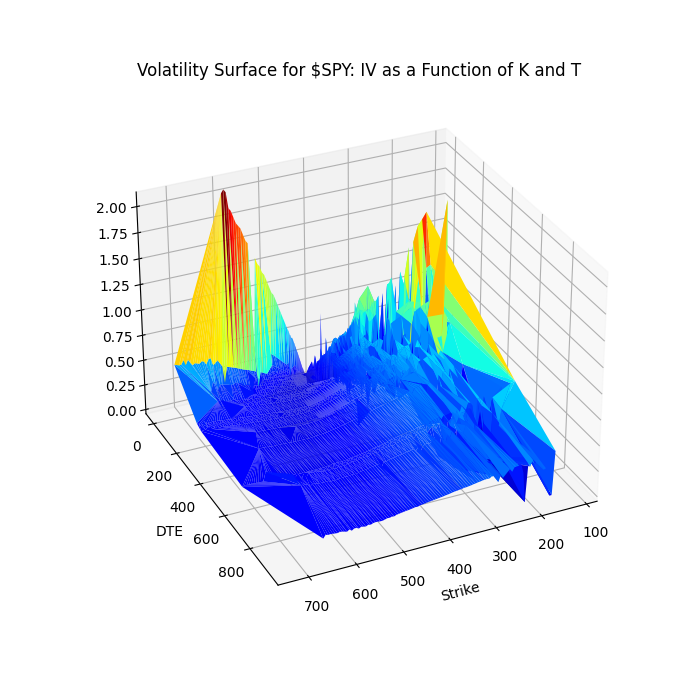
\includegraphics[width=4.49618in,height=4.49618in]{media/media/image1.png}
  \caption{3D Volatility Surface}
  \label{fig:image1}
\end{figure}


As the mathematics of volatility modelling evolved researchers
questioned the assumption of Geometric Brownian Motion (GBM). GBM
assumes that the process has no memory i.e., each step is a Markovian
process, so the noise has zero autocorrelation. If that assumption is
true, then according to Itô calculus the standard deviation of price
changes scales with the square root of time. However, if the volatility
increments are positively and/or negatively correlated, then volatility
process has memory and time--series behaviour cannot be modelled by GBM.

Thus, the researchers turned to another type of Brownian motion ----
fractional Brownian motion (fBm). Fractality of the object means that it
does not change its form at different scales (scale can mean distance,
time). These are self-- similar objects, where we can zoom in and out and
note that the shapes will be approximately the same. In the example of
volatility time series, if we look at intraday or weekly patterns, we
will roughly see the same shape.

It was not until Gatheral et al., \cite{gatheral2014volatility_3} seminal paper that the idea of
roughness in volatility modelling took off. Their work introduced the
concept of rough volatility, where volatility evolves as a fractional
process with a Hurst exponent less than $\frac{1}{2}$, challenging the conventional
assumption of smoothness implied by GBM. In their paper, the authors
showed the first applications in both pricing and volatility
forecasting, as well as established a rigorous theory as to why
volatility exhibits roughness. This development occurred several decades
after the introduction of fractional Brownian motion by Mandelbrot and
Van Ness \cite{ness1968fractional_4}. According to the new theory that volatility is rough,
the roughness lies in the market microstructure and order flow
distribution and behaviour. The wide proliferation of high frequency
trading simply exacerbates these effects. The theory behind this is that
buy orders generate more buy orders, and vice versa. However, the
cascade of sell orders often has more impact on the order book and
through feedback loop on the underlying spot market. This is what
economists typically refer to as boom--and--bust cycles or reflexivity
between processes. There are other more nuanced volatility dampening
effects such as order splitting, but this is not the scope of this
paper.

Also referred to as statistical volatility, historical volatility (HV)
is a backward--looking measure that quantifies the extent of past price
fluctuations over predetermined time intervals. In contrast to implied
volatility, which incorporates expectations of future uncertainty, HV
relies solely on historical data and thus provides no direct insight
into future market conditions. Because of this retrospective focus, HV
is less commonly used as a predictive tool. Nonetheless, changes in HV
remain informative: an increase often signals that the security's price
has recently undergone more pronounced movements------suggesting a possible
shift in market dynamics------while a decrease implies that some
uncertainty has been resolved, allowing prices to stabilize and
potentially revert to their long--term averages.

While fractional and rough volatility models attempt to capture the
complex nature of volatility dynamics, practitioners often rely on
market--derived measures such as the VIX and VVIX. As stated earlier,
CBOE Volatility Index (VIX) is a real--time measure of the market's
expectations of the near--term changes in the S\&P 500 index. The index
is derived from the prices of at the money and out of the money SPX
index options with near--term expiration dates. The calculation derives a
30--day forward projection of volatility. In financial markets,
volatility is a measure of how fast prices change and measures the
degree of fear or greed amongst the market participants.

In 2012, CBOE introduced a new index called VVIX or volatility of
volatility. The VVIX index is a volatility of volatility measure as it
represents the expected volatility of the 30--day forward price of the
CBOE Volatility Index (the VIX). It is this expected volatility that
drives the price of the VIX options. VVIX is calculated from the price
of a portfolio of liquid at--the--money and out--of--the money VIX options.

Having introduced both VIX and VVIX, we now turn to the range of
modelling techniques that this study will employ. These methods were
chosen to capture the multifaceted nature of volatility, incorporating
memory, non--normality, and scale--invariance. We will use various
algorithms to model VIX and VVIX: (i) Naïve Models (ii) GARCH family,
(ii) Monte Carlo, (iii) LSTM, (iv) SVM, (v) Random Forest Regressor and
more modern approaches encompassing (vi) NBEATS (vii) MSM, (viii) MMAR,
(ix) RL (x) GAN and (xi) Mixed Fuzzy Fractional Brownian motion.

As one of the parameters that influences the movement in stock prices,
volatility is a crucial input to numerous financial market operations,
and it becomes an important tool to assess the risk of ruin for
portfolio managers, investors, and other interested parties \cite{poon2003forecasting_5}. The
modelling of volatility is a complex task because it cannot be observed
directly. Indeed, it can only be measured by looking at the extent of
the movement of the option prices and deriving it mathematically from
that.

The mathematical estimators are complicated also by volatility clusters,
fat tails, non--normality of the distribution, and structural breaks in
the distribution of the returns. These features cannot be captured by
simple classical models such as the autoregressive moving average (ARMA)
process.

The next chapters will present an overview of the main estimators of
the volatility with particular attention to the heteroskedastic models.

\hypertarget{research--question--and--postulated--hypothesis}{%
\section{\texorpdfstring{\textbf{RESEARCH QUESTION AND POSTULATED
HYPOTHESIS}}{RESEARCH QUESTION AND POSTULATED HYPOTHESIS}}\label{research--question--and--postulated--hypothesis}}

This research investigates three primary research questions and their
corresponding hypotheses.

\begin{enumerate}
\def\labelenumi{\roman{enumi}.}

\item \textbf{Research Question 1:} To what extent do volatility time series and their first derivatives (VVIX) exhibit fractal properties, and can these characteristics be accurately modelled using mixed fuzzy fractional Brownian motion (mfFBm)?

\textbf{Hypothesis:} The central hypothesis is that both the volatility time series and its first derivative (the ``volatility of volatility'' or VVIX) exhibit fractal properties. Fractality implies self--similarity across different time scales, meaning that these time series cannot be accurately modelled using classical diffusion laws, such as Fick's laws, which assume memoryless and random--walk behaviours. In fractal processes, the Hurst exponent (H) plays a crucial role. If H \textgreater{} $\frac{1}{2}$, the time series displays long--range dependence (persistence), so high volatility today suggests it will likely remain high in the near future. Conversely, if H \textless{} $\frac{1}{2}$, the series is anti--persistent (rough), and increases in volatility tend to be followed by decreases, reflecting negative autocorrelation. The time series is more erratic and less smooth. For example, a market where volatility changes rapidly and frequently, with no clear trend over time. Empirical evidence often shows that H $\neq$ $\frac{1}{2}$, indicating that simple random--walk assumptions do not hold. To capture these fractal characteristics, this thesis develops the necessary theoretical framework required to forecast volatility by first forecasting its derivative (VVIX). This derivative quantifies the fractal dimension of the time series, providing insight into its degree of self--similarity. The higher the fractal dimension, the more self--similar the time series is. Building on the foundational work of Mandelbrot, Lux, Liu, and Calvet, we extended a novel mathematical process------mixed \emph{fuzzy} fractional Brownian motion (mfFBm) [P1] [P2] [P3] [P4] that incorporates both fuzziness and jump processes into fractional Brownian motion.

\item \textbf{Research Question 2:} Does the fractal nature of volatility imply significant time--scale invariance, and can a theoretical framework be developed to capture these repeating statistical patterns?

\textbf{Hypothesis:} The second hypothesis proposes that, due to the observed fractal nature of volatility, a degree of time--scale invariance should exist, meaning that statistical patterns repeat across different scales. The empirical findings in this thesis regarding the shifting Hurst exponent and the success of fractal based modelling in the literature support this proposition. This motivates the development of a scale--invariant theoretical framework as a core goal of this research.

\item \textbf{Research Question 3:} How does the proposed fractal--based theoretical framework compare in forecasting performance against traditional econometric and deep learning models?

\textbf{Hypothesis:} Finally, we hypothesize that the novel theoretical approach will outperform conventional techniques. We compare our results to more traditional econometric and deep learning models as discussed in [P1] [P4] and [P3]. This comparison of conventional techniques establishes a performance benchmark, which serves to justify the need for the novel theoretical approach developed in this thesis.

\end{enumerate}

\hypertarget{contribution--to--knowledge}{%
\section{\texorpdfstring{\textbf{CONTRIBUTION TO
KNOWLEDGE}}{CONTRIBUTION TO KNOWLEDGE}}\label{contribution--to--knowledge}}

The aims of this research are threefold. First,
state--of--the--art methods related to fuzzy fractional Brownian motion are reviewed to establish the theoretical soundness of these approaches. Second, 
extension and refinement of several recent theoretical results are presented, providing novel proofs and extensions [P2] [P3]. Third, empirical evidence demonstrating the practical performance of
various modelling techniques is presented. In undertaking this work, a
narrative review methodology is employed to synthesise existing research and
identify areas where the proposed framework can contribute new
perspectives. This approach enables a comprehensive overview of the
literature, as well as expert interpretation and synthesis, both of
which are essential for advancing theoretical frameworks and introducing
novel proofs in this domain.

This thesis develops a unified framework that integrates fractional
Brownian motion with fuzzy processes, resulting in a product measure
space encompassing both the intrinsic randomness of fractional Brownian
motion and the fuzziness of associated parameters [P2] [P3].
Although existing literature provides numerous insights into forecasting
the VIX time series directly, our research develops the theoretical
foundation for a novel approach where VIX could be forecasted through
its first derivative, VVIX, using fractional calculus techniques
developed herein and combine them with fuzzy sets and jump processes.
Since the VIX represents implied volatility rather than a direct price
series, it behaves differently from standard financial time series. We
hypothesize that by focusing on VVIX and employing multifractal
models------such as the Multifractal Model of Asset Returns (MMAR) and its
Markov--switching multifractal (MSM) variant enhanced with fuzzy
variables------we can improve forecasting accuracy. This approach
contributes uniquely to the existing body of knowledge on VIX
forecasting by providing a new theoretical framework and a proposed
methodology for its application, as these techniques have rarely been
explored in this context.

The scarcity of research and literature on fractional mathematical
methods in finance, particularly regarding volatility modelling,
indicates that this area remains significantly under--researched. This
work thus fills a critical gap, laying the groundwork for further
exploration and development of fuzzy fractional approaches in the
financial domain.

\hypertarget{document--structure}{%
\section{\texorpdfstring{\textbf{DOCUMENT
STRUCTURE}}{DOCUMENT STRUCTURE}}\label{document--structure}}

The remainder of this thesis is structured as follows. Chapter 2 serves
as the literature review chapter, providing a detailed theoretical
overview of the proposed models. It begins by discussing the fractal
nature of financial data and multifractal models (e.g., MMAR), and then
progresses through various volatility forecasting techniques, including
GARCH, LSTM, Monte Carlo simulations, Support Vector Machines, Random
Forest Regressor, NBEATS, Reinforcement Learning, GANs, and Fuzzy Neural
Networks. 

Chapter 3 focuses on data and methodology. It introduces smoothing and
transforming techniques, tests for stationarity using the Augmented
Dickey--Fuller test, and outlines the methodology for generating
multifractal simulations to better understand complex market behaviour.
In addition to reviewing these methods, Part 3 also includes a
dedicated section presenting the results of these models, detailing the
performance and clustering techniques employed (K--Means and Fuzzy
C--Means) and exploring deep neural network applications.

Chapter 4 presents the evaluation metrics used to assess the forecasting
models, while Chapter 5 delves into the mixed fuzzy fractional Brownian
motion (mfFBm) framework with jumps. This includes theoretical
preliminaries, handling cases where H \textgreater{} $\frac{1}{2}$ and H \textless{}
$\frac{1}{2}$, introducing fuzziness and jump processes, and providing rigorous
proofs and applications.

Chapter 6 presents conclusion and future work, summarises the key research findings, discusses their implications for volatility modelling, acknowledges the study's limitations, and suggests potential avenues for future research.
Finally, the thesis concludes with appendices containing code samples
(e.g., for the Augmented Dickey--Fuller test and multifractal
simulations), table A3 mapping the results and models to Hurst parameter
regimes and a comprehensive list of references.

\hypertarget{chapter--2--literature--review}{%
\chapter{\texorpdfstring{\textbf{CHAPTER 2 -- LITERATURE
REVIEW}}{CHAPTER 2 -- LITERATURE REVIEW}}\label{chapter--2--literature--review}}

\hypertarget{introduction--1}{%
\section{\texorpdfstring{\textbf{
INTRODUCTION}}{INTRODUCTION}}\label{introduction--1}}

An accurate model should be subjected to rigorous testing and adhere to
the principle of parsimony, which holds that models with fewer
parameters are generally preferable \cite{taylor2008modelling_10}.

Measuring and forecasting volatility has attracted considerable
attention from both academia and market practitioners ever since the
Chicago Board Options Exchange (CBOE) introduced the VIX in 1993. In
2003, the methodology for calculating the VIX was revised in
collaboration with Goldman Sachs, resulting in a widely accepted measure
of expected volatility that has since been extensively used by scholars,
traders, and risk managers. When volatility is interpreted as
uncertainty, it becomes a key input in portfolio investment decisions,
especially for pricing derivative instruments such as options. In 1996,
the Basel Accord began requiring the modelling and forecasting of
volatility as a mandatory input to risk management for financial
institutions worldwide.

Ruipeng Liu and Rangan Gupta \cite{liu2022investors_11} studied the role of investor
uncertainty as measured by the conditional volatility of investor
sentiment in forecasting the volatility of six major stock markets using
a bivariate Markov--switching multifractal (MSM) model. Their results
showed that incorporating information on investor uncertainty led to
smaller forecasting errors compared to univariate MSM models that did
not include this metric. This superior performance underscores the
importance of accounting for long memory and structural breaks when
forecasting stock market volatility. Moreover, since financial market
volatility is influenced by investor uncertainty, policymakers should
recognize that such uncertainty can prolong negative economic impacts
through feedback loops affecting real macroeconomic variables, as well
as delaying investment and consumption decisions.

C--Rene Dominique and Luis Eduardo Solis Rivera \cite{solis2011mixed_12} studied
short--term and long--term dependence of the S\&P500 index using a mixed
fractional Brownian motion (mfBm) model. The mfBm model is a
continuous--time stochastic process and is generalisation of the
fractional Brownian motion (fBm) model that allows for both short--term
and long--term dependence. The process is characterised by two Hurst
parameters, H\textsubscript{S} and H\textsubscript{L}.
H\textsubscript{S} measures the short--term dependence, and
H\textsubscript{L} measures the long--term dependence. By capturing both
volatility clustering and heteroscedasticity, mfBm better represents
market microstructure noise in the short run and macroeconomic factors
such as interest rates and inflation in the long run. The authors found
that long--term dependence in the S\&P 500 index is stronger during
periods of economic expansion than during recessions.

In 2012, the CBOE introduced the Volatility of Volatility Index (VVIX),
often referred to as ``vol of vols.'' VVIX is calculated in a manner
similar to VIX, except that it uses the VIX time series instead of S\&P
500 options. VVIX measures the expected volatility of the VIX itself.
This chapter reviews academic studies focusing on various volatility
forecasting models including GARCH, Monte Carlo simulations, Support
Vector Machines, LSTM, Random Forest, and other state--of--the--art
techniques. While much of the existing literature focuses on forecasting
VIX, there is a relative scarcity of research on forecasting VVIX using
modern approaches such as fractal methods, deep reinforcement learning,
or GANs. Some studies have explored Bayesian methods and Markov chain
Monte Carlo (MCMC) techniques for forecasting VVIX, but overall, this
remains an under--researched area.

\hypertarget{fractal--nature--of--the--data}{%
\subsection{FRACTAL NATURE OF THE
DATA}\label{fractal--nature--of--the--data}}

The central thesis of this paper is that volatility and its first
derivative time series data are fractal. In other words, if we examine
monthly, weekly, daily, or tick--level data, we would not be able to
distinguish one timescale from another unless we already know the time
frame. While there are cut--off points that theoretically allow one to
differentiate between scales, these points are often so minuscule (e.g.,
fractions of a nanosecond) or so vast (e.g., multiple decades) that we
choose to disregard them in practical applications.

Mathematicians have long recognised discrepancies between standard
Brownian motion models and real financial data. Firstly, the data
exhibit temporal dependence, with periods of large changes alternating
with periods of small changes. Secondly, the tails of the return
distribution are far fatter than those predicted by a Gaussian
distribution. Although the data may become less peaked and have thinner
tails as the sampling interval extends to decades, they never truly
become Gaussian. Empirical studies indicate that multifractal processes
never converge to a Gaussian distribution. Consequently, researchers
have explored alternative distributions and approaches such as the
Student's t--distribution, Poisson jumps, and nonparametric
representations to better capture these characteristics.

GARCH(p, q) models, introduced by Bollerslev, address volatility
clustering and help mitigate the issue of fat tails. In these models, a
higher $\alpha$ coefficient tends to produce sharper changes in volatility,
while $\beta$ corresponds to more gradually evolving volatility dependencies.
Since ($\alpha$ + $\beta$) \textless{} 1 typically holds, there is a trade--off
between immediate large changes and sustained long cycles in volatility.
This limitation means that GARCH cannot simultaneously capture abrupt
shifts and prolonged volatility patterns.

Multifractality was introduced by Mandelbrot in 1972 and was first
applied in physics to describe distributions of energy and matter such
as minerals, turbulent dissipation, stellar matter. Mandelbrot extended
multifractality to measure the heterogeneity in the financial time
series and extended it to stochastic processes. Most diffusions are
characterised by increments that grow locally at the rate
($\Delta$t)\textsuperscript{1/2} throughout their sample path. The exception
is FBM which has growth rate ($\Delta$t)\textsuperscript{H}, where H is
invariant with t. Multifractals, on the other hand, have a multiplicity
of local growth rates for increments (where h = 1/2 , this becomes
normal Brownian motion).

Mandelbrot's seminal 1997 paper introduced the Multifractal Model of
Asset Returns (MMAR), viewing asset prices as multiscaling processes
with both long memory and heavy tails. In the MMAR, volatility of
volatility is introduced via a random trading time, generated as the
cumulative distribution function of a random measure. Under this
framework, the distribution of returns and volatility remains invariant
across time scales, and the compounding effect of random trading time
allows direct modelling of variance without influencing the direction or
correlation of increments. In other words, the introduction of random
trading time T(t) in the Multifractal Model of Asset Returns (MMAR)
allows direct modelling of time--varying variance. This is achieved by
scaling the variance through T(t) without altering the underlying
direction (sign) or correlation structure of the price increments, which
remain determined by the properties of the driving process (e.g.,
Brownian or fractional Brownian motion).

In their seminal paper, Thomas Lux and Ruipeng Liu \cite{lux2017generalized_14} extended
Generalised Method Moment (GMM) approach of Lux (2008) to multivariate
settings and applied it to discrete and continuous distributions of the
volatility components. Their results showed that the performance of the
GMM estimator remained robust when moving from univariate to bivariate
or trivariate models. In subsequent work, Ruipeng Liu et al \cite{liu2019volatility_15}
utilised a bivariate Markov--switching multifractal (MSM) model to
examine the interplay between exchange rates and stock market volatility
in various developed (Canada, France, Germany, Italy, Japan, UK) and
emerging (BRICS) economies. The MSM model captured key statistical
anomalies in volatility dynamics. The authors compared GARCH models with
MSM and found that GARCH offered superior volatility forecast for short
horizons whereas multifractal models offer significant improvements for
longer horizons across most markets. Bivariate model outperformed
univariate model across developed markets but had mixed performance in
emerging markets.

\hypertarget{fractals}{%
\subsubsection{FRACTALS}\label{fractals}}

A fractal is defined as a curve or geometric shape, each part of which
has the same statistical properties as the whole. Fractals are used in
modelling structures such as eroded coastlines and snowflakes in which
similar patterns recur at progressively smaller scales, and in
describing partly random or chaotic phenomena such as crystal growth,
fluid turbulence, and galaxy formation. Fractals are created by
repeating a simple process in a never--ending feedback loop. A fractal
dimension of 1D time series embedded in a 2D plot measures the roughness
of a surface and has the following simple relationship with hurst
exponent in 2D space: \(d_{H} = 2 - H\)\emph{.} It is defined as the
Hausdorff dimension, which is the dimension of a fractal set, is
inversely related to the Hurst exponent (H) which is a measure of the
long--term dependence of a time series. This relationship can be
explained in the following way. A time series with a high Hausdorff
dimension is said to be ``rough'', meaning that it has a lot of
small--scale variations. A time series with a low Hausdorff dimension is
said to be smooth, meaning that it has few small--scale variations. Hurst
exponent is defined as the exponent of the power law that describes the
decay of the autocorrelation function of the time series. In other
words, The Hausdorff dimension, d\textsubscript{H}, describes how a
fractal curve fills space, offering insights into its roughness and
detail across scales. For instance, when \emph{d\textsubscript{H} =1,}
the curve is smooth and resembles a straight line. Conversely, if
\emph{d\textsubscript{H} =2,} the curve becomes so jagged that it
effectively fills an entire two--dimensional plane, like an irregular
coastline. The relationship \(d_{H} = 2 - H\) establishes a connection
between the smoothness of the curve and its fractal dimension. As the
Hurst exponent H increases, the curve becomes progressively smoother,
and the fractal dimension d\textsubscript{H} decreases, indicating
fewer small--scale variations.

In time series analysis, the Hurst exponent \emph{H} governs the
behaviour of a process over time. If \emph{H\textgreater0.5,} the series
is persistent, meaning trends tend to continue in the same direction,
creating smoother, long--range dependent paths. At \emph{H=0.5}, the
series behaves like a random walk, exhibiting no memory and resembling
standard Brownian motion with \emph{d\textsubscript{H} =1.5.} For
\emph{H\textless0.5}, the series is anti--persistent, where trends tend
to reverse frequently, resulting in rougher, more erratic paths with
\emph{d\textsubscript{H} \textgreater1.5}. Thus, the relationship
\(d_{H} = 2 - H\) maps the persistence or anti--persistence of time
series to their geometric roughness.

The physical interpretation of this relationship differs between
fractals and time series. In fractals, the Hausdorff dimension
quantifies the spatial roughness of a curve, reflecting how its
complexity changes as one zooms in to finer scales. In time series, the
Hurst exponent measures the persistence or memory of increments over
time, linking temporal behaviour to spatial roughness. Despite these
different contexts, the mathematical relationship bridges the two
domains, providing a geometric interpretation of time series roughness
while offering a quantitative measure of the self--similar nature of
fractals and their temporal equivalents.

\begin{figure}[htbp]
\centering
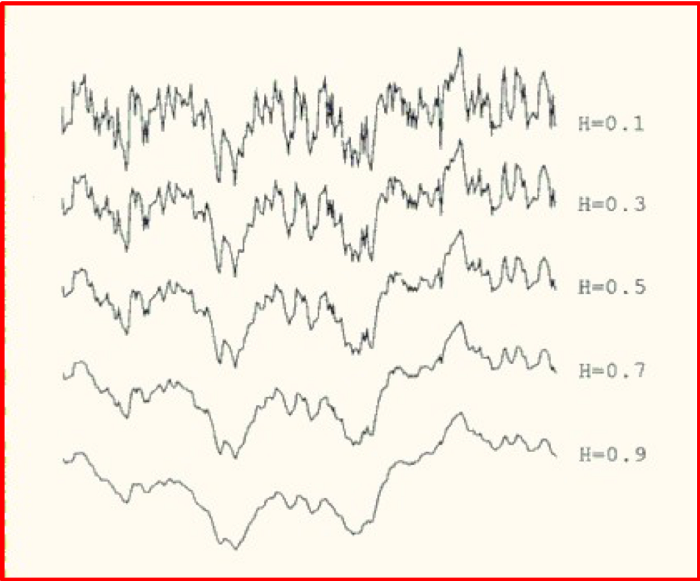
\includegraphics[width=3.56135in,height=2.95349in]{media/media/image2.png}
\caption{Source: \cite{saupe1988algorithms_16} Hurst exponents and roughness.}
\label{fig:hurst-roughness}
\end{figure}


Figure 2.1 \cite{saupe1988algorithms_16} illustrates how the Hurst exponent \emph{H}
influences the roughness of a time series. As \emph{H} increases, the
curves become smoother, indicating fewer small--scale variations. This
corresponds to smaller fractal dimensions
\emph{d\textsubscript{H}}\hspace{0pt}, where the relationship
\(d_{H} = 2 - H\) holds. Fractals exhibit statistical self--similarity,
meaning that subsets of the process resemble the full set when viewed at
different scales. A Hurst exponent measures the diffusion speed of the
series. The problem with simulating even a high Hurst exponent is that
on its own, it still produces a Gaussian distributed random walk and
with the assumption of Levy stable distributions that imply an infinite
variance, which can exhibit randomness, is that the key feature of the
data is lost i.e. the sporadic nature of volatility which tends to go
wild for some time and show multi sigma moves for several days in a row,
and then abruptly go back to low periods of volatility. To replicate
market panics, it is simply not enough to generate a leptokurtic
distribution that generates high kurtosis occasionally, it also must
cluster these days together.

\hypertarget{long--range--dependence}{%
\subsubsection{LONG RANGE DEPENDENCE}\label{long--range--dependence}}

Processes that have long range dependence occur when past events are
nontrivially correlated with future events, even if they are far apart
and exhibit a high persistence degree. This persistence arises from a
slow, power--law decay in the autocorrelation function rather than the
exponential decay seen in short--memory processes. One example by
Granger, Joyeux and Hosking \cite{robinson2003time_17} is given by following a
fractionally differenced time series:

\begin{equation}
(1 - L)^{d} S_{t} = \varepsilon_{t}, \qquad d \notin \mathbb{Z}.
\end{equation}


where \emph{L} is the lag operator shifting \emph{S\textsubscript{t}} to
\emph{S\textsubscript{t-1}}, the exponent \emph{d} is non--integer that
determines the degree of fractional differencing, and $\epsilon$ is a white noise
error term. Fractional differencing allows for long--memory behaviour,
where correlations decay slowly, following a power--law function, as
opposed to traditional short--memory processes.

\hypertarget{hurst--exponent--as--a--measure--of--diffusion}{%
\subsubsection{HURST EXPONENT AS A MEASURE OF
DIFFUSION}\label{hurst--exponent--as--a--measure--of--diffusion}}

To understand the nature of the price series it is helpful to analyse
its speed of diffusion. Diffusion measures the spread of the series from
a location where its concentration is higher than in most other places.
It can be measured by examining how the variance of displacements scales
with the time lag $\tau$:

\begin{equation}
\operatorname{var}(\tau)=\left\langle \left|x_{t+\tau}-x_t\right|^2 \right\rangle .
\label{eq:var-tau}
\end{equation}


where $\tau$ is the time interval between measurements,
\emph{x\textsubscript{t}} represents the log--transformed series \emph{x
= log S(t}), and $\langle$$\cdot$$\rangle$ denotes an average over time. Log transformations
are often applied to stabilise variance and reduce heteroskedasticity in
the series.

The mean squared displacement (MSD) is a measure of the deviation of the
position of the particle with respect to a reference position over time.
It is the most common measure of the spatial extent of random motion and
is calculated as the average of the squared displacements of the
particle over a given time interval. MSD behaves differently depending
on the type of diffusion. In the case of normal diffusion, the MSD
scales linearly with time, MSD$\sim$$\tau$, which is typical of a random walk with
no memory or persistence. For subdiffusion, the MSD grows slower than
linearly, scaling as MSD $\sim$ \emph{$\tau$\textsuperscript{H}}, where \emph{H}
\textless{} 0.5. This indicates anti--persistence, meaning the series
exhibits rough behaviour with frequent trend reversals. In contrast,
superdiffusion occurs when the MSD grows faster than linearly, following
MSD$\sim$ \emph{$\tau$\textsuperscript{H}}, where \emph{H \textgreater{} 0.5}.
Superdiffusion reflects persistent behaviour, where trends tend to
continue in the same direction, resulting in a smoother and more
predictable trajectory.

\begin{figure}[!htbp]
\centering
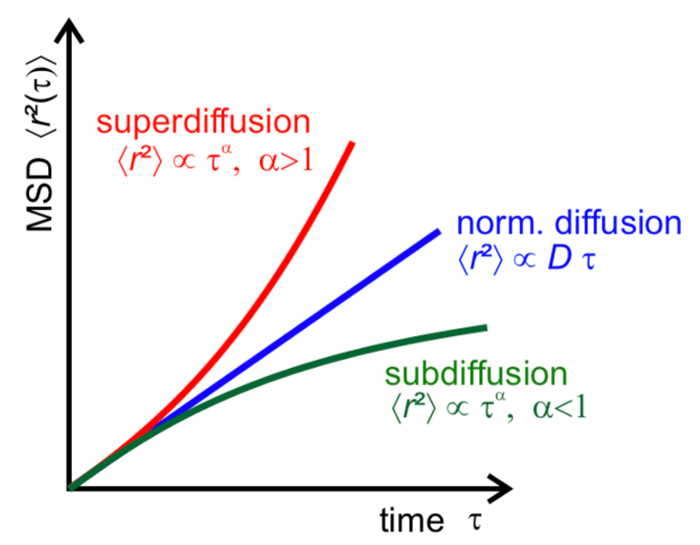
\includegraphics[width=0.55\linewidth]{media/media/image3.png}
\caption{Source: \cite{sadhukhan2020avascular_18} Relationship between Mean Squared Displacement and Time.}
\label{fig:msd-time}
\end{figure}

For example, Figure 2.2 illustrates the MSD for Brownian motion
will increase linearly with time, while the MSD for a system with
anti--persistence and frequent trend reversals will increase more slowly
than linearly \cite{sadhukhan2020avascular_18}.

Volatility of asset return time series strongly depends on the frequency
one chooses to measure it. Measurement at one--minute intervals differ
significantly from daily variance. Empirically, it has been established
that if returns follow a Geometric Brownian Motion (GBM), the variance
increases linearly with the lag $\tau$, and the returns are normally
distributed. On the other hand, if there are even small deviations from
a pure random walk as is often the case, the variance for lag $\tau$ is not
proportionate to $\tau$ anymore but instead follows a power--law relationship:

\begin{equation}
\operatorname{var}(\tau) \propto \tau^{2H}.
\label{eq:var-tau-hurst}
\end{equation}


where \emph{H} is the Hurst exponent. For trending assets \emph{H}
\textgreater{} $\frac{1}{2}$ indicating positive persistence and for mean reverting
assets \emph{H}\textless{} $\frac{1}{2}$, indicating negative persistence. The Hurst
exponent measures the level of persistence of a time series. The level
of persistence is a measure of how likely it is to continue in its
current trend. A time series with high persistence is more likely to
continue in its current trend, while a time series with low persistence
is more likely to reverse its trend. If \emph{H = $\frac{1}{2}$} then the time
series has no persistence and follows a Geometric Brownian Motion which
is defined by the following process
\(X(t) = \ X(0)*\ exp\left( \mu t\  + \ \sigma W(t) \right),\) where
\emph{W(t)} is a standard Brownian motion, \emph{$\mu$} is the drift term,
and \emph{$\sigma$} is the volatility. GBM has a few properties that makes them
easy to use such as the distribution of the underlying
is lognormal, the process is a martingale, so it is memoryless, and the
underlying is always positive. The last property is not necessary if we
use Arithmetic instead of Geometric Brownian motion because the
underlying processes are quite often negative. Both Arithmetic and
Geometric Brownian Motions are quite popular because they give easy
closed form solutions, but they are a very simplified model of reality
and in our view unsuitable for making real life decisions under
uncertainty. The real world is far more complex than GBM, and there are
many other filtrations that affect the underlying processes. Examples of
each case of persistent, antipersistent and GBM are illustrated in below
diagrams.

\begin{figure}[htbp]
\centering
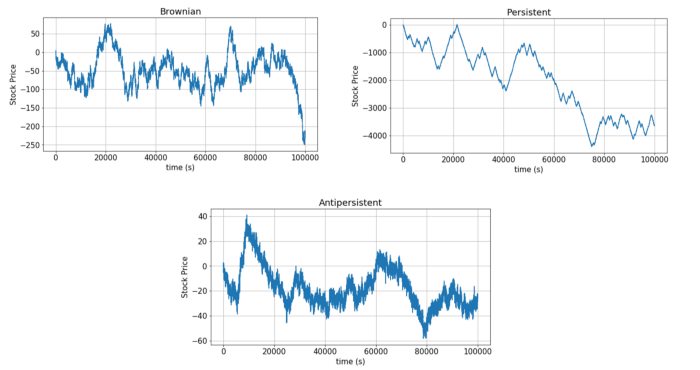
\includegraphics[width=0.95\linewidth]{media/media/image4.png}
\caption{Source: \cite{sibirtsev2019how_19} Different Levels of Persistence.}
\label{fig:persistence-levels}
\end{figure}


\hypertarget{autocorrelation}{%
\subsubsection{AUTOCORRELATION}\label{autocorrelation}}

The autocorrelation function measures the linear relationship between a
time series and its lagged values and is defined as follows:

\begin{equation}
\rho(\tau)=\frac{1}{\sigma^{2}} \, \mathbb{E}\!\left[\left(S_t-\overline{S}\right)\left(S_{t+\tau}-\overline{S}\right)\right].
\label{eq:autocorr}
\end{equation}


where \emph{$\sigma$\textsuperscript{2}} is the variance of the series,
\emph{E} is the expectation operator, and $\tau$ is the lag.

Processes with autocorrelations that decay slowly are termed long memory
processes, meaning past events nontrivially influence future events even
over large lags. Such processes have some memory of past events which
have diminishing influence on future events.

Long memory processes are characterised by autocorrelation function with
power--law decay:

\begin{equation}
\rho(\tau \to \infty) \propto \tau^{-\alpha}.
\label{eq:rho-power-law}
\end{equation}


where \emph{$\alpha$ \textgreater0}. The relation between \emph{a} and \emph{H}
is given by \emph{a = 2(1--H)} and as \emph{H} $\rightarrow$ 1, the decay becomes
slower since \emph{a} approaches zero indicating persistent behaviour.
These processes where H is greater than $\frac{1}{2}$ but less than 1 are long
memory processes and are often referred to as Fractional Brownian motion
(FBM). The value of H strongly depends on the choice of lags $\tau$.

\hypertarget{multifractal--model--of--asset--returns--mmar}{%
\subsection{MULTIFRACTAL MODEL OF ASSET RETURNS
(MMAR)}\label{multifractal--model--of--asset--returns--mmar}}

Unlike earlier versions which focused on L--stable distributions, MMAR is
a generalisation of the L--stable distribution model and the fractional
Brownian motion model. It combines long tails and finite variance of the
L--stable distribution model with the long dependence of the fractional
Brownian motion model over discrete sampling intervals. Secondly, the
MMAR contains long dependence which is the characteristic feature of
Fractional Brownian Motion (FBM), which was formally introduced by
Mandelbrot and van Ness in 1968 \cite{ness1968fractional_4}. Finally, the last feature of
MMAR is the concept of trading time, introduced by Mandelbrot and Taylor
in 1967 \cite{taylor1967distribution_20}. This time concept is the explicit modelling of the
relationship between clock time which we can observe and measure, and
unobserved natural timescale of the returns process. They argued that
the time at which trades occur is not evenly spaced but rather is
clustered around certain times. This clustering of trades leads to a
distortion of clock time. The MMAR takes into account the concept of
trading time by modelling the return process as a function of trading
time. This allows the model to capture the clustering of trades and
distortion of clock time. All three features are contained in MMAR which
accounts for empirical observations of financial time series with long
tails relative to normal distribution and long memory in the absolute
value of returns and volatility. Stochastic fluctuations in volatility
are measured by a random trading time.

Multifractals are used in MMAR model by generating a multiplicative
cascade. A multiplicative cascade is a process in which a set of
intervals is split into smaller intervals, and the sizes of the smaller
intervals are determined by a random multiplicative process. For
instance, at each stage of the cascade, intervals can be split in
\emph{b \textgreater{} 2} intervals of equal size. Subintervals, indexed
from left to right by \emph{$\beta$ (0$\leq$ $\beta$ $\leq$ b--1)} receive fractions of the
total mass equal to \emph{m\textsubscript{0,} m\textsubscript{b--1.}} The
term ``mass'' in the context of MMAR model mass is not the same as
probability mass. In the MMAR model, mass refers to a conceptual measure
used to describe how the total quantity (e.g., volatility intensity or
some scaling factor) is distributed across progressively smaller time
intervals. This can be thought of as the total number of particles, or
the amount of energy in the system (probability mass refers to the
probability that a particular outcome will occur e.g., the probability
mass of rolling 6 on a die is 1/6).

In MMAR, the mass of each interval is multiplied by a random factor. The
random factors are chosen so that the total mass of the system is
preserved. By the conservation of mass, the total mass of the system
must remain constant over time, so these fractions add up to 1:
\emph{$\sum$m($\beta$) = 1}. For example, the line at step 0 starts with a mass of
10,000. At each step, the line is divided into two sections, one of
which will have its mass multiplied by 0.6, and the other by the left
over 0.4 At the next step, these two sections are divided into two
further sections, for a total of 4, and the same multiplication is
applied to it. This means that the probability mass of each interval is
not affected by the multiplicative cascade process. In other words, the
probability mass of each interval is independent of the mass of the
interval. This is an important distinction because it means that the
MMAR model can be used to model systems where the probability mass of
each outcome is not constant.

By applying multiplicative cascade process at finer and finer time
scales, we end up with a pattern where volatility is distributed
unevenly. Some very short intervals might receive disproportionately
high ``mass`` (intense volatility), while neighbouring intervals receive
less. Over time, this uneven distribution across scales creates a
multifractal structure------one that closely resembles the clustering of
high and low volatility periods observed in real financial markets.

One can also introduce randomness to this process when generating these
cascades by assigning a random multiplicative factor to each interval.
The multiplicative cascade process divides the line smaller and smaller
intervals, and then multiplies the mass of each interval by a random
factor. The random factors are chosen so that the total mass of the line
is preserved. This means that the total mass of the system is always the
same, even though the mass of individual intervals may change. A simple
analogy to understand this concept of mass in MMAR is a bag of marbles.
The total mass of marbles in the bag is constant. We can divide the
marbles into smaller and smaller groups, but the total mass of the
marbles will always be the same. This is similar to the way the total
mass of the system is preserved in the MMAR model. Figure 2.8 illustrates an example of a basic
deterministic multiplicative cascade. 

\begin{figure}[htbp]
\centering
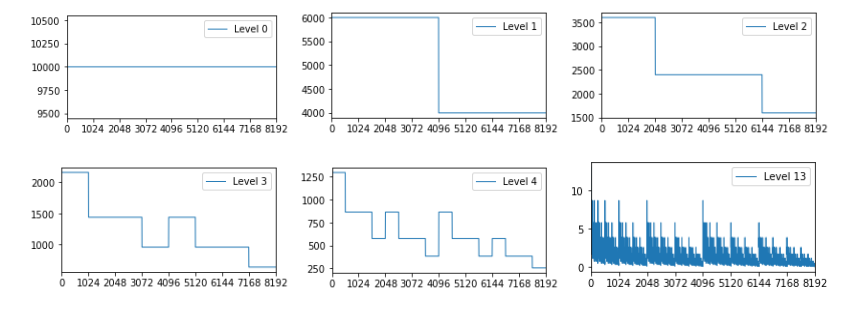
\includegraphics[width=0.95\linewidth]{media/media/image9.png}
\caption{Source:  \cite{sibirtsev2019how_19} Multiplicative cascade.}
\label{fig:multiplicative-cascade}
\end{figure}


Volatility clustering is the tendency for periods of high volatility to
follow other and vice versa. The MMAR model, due to its multifractal
construction and integration of trading time and long--range dependence,
has been shown to be an effective tool in modelling this phenomenon. By
capturing both long--term dependence and the hierarchical distribution of
volatility across different time scales, MMAR aligns closely with the
empirical behaviour of asset returns.

\hypertarget{trading--time--and--compound--processes}{%
\subsubsection{TRADING TIME AND COMPOUND
PROCESSES}\label{trading--time--and--compound--processes}}

According to MMAR, the price change of an asset is considered a function
of both the passage of trading time and random movements known as
Brownian motion. Price is a function of trading time which is a function
of clock time. So, the two functions of time and Brownian motion work
jointly to produce a model different from its two composition parts. By
combining these two components, MMAR aims to provide a more
comprehensive representation of asset returns, that accounts for both
the temporal structure of trading and the inherent randomness in market
dynamics. Mandelbrot presented rigorously the concept in his 1997 paper
``A Multifractal Model of Asset Returns'' \cite{mandelbrot1997multifractal_13}. Following
Mandelbrot's notation, MMAR is defined as:

\begin{equation}
X(t) = \ln P(t) - \ln P(0).
\label{eq:log-price-increment}
\end{equation}


where \emph{P(t)} denotes a point \emph{P} at time \emph{t} and
\emph{P(0)} is the point at time zero. If \emph{H = 0.5}, then these
price movements are mutually independent, isotropic, and the price
process is Brownian Motion.

\textbf{\uline{Assumption 1}}

\begin{equation}
X(t) \equiv B_H\!\bigl[\theta(t)\bigr].
\label{eq:subordination}
\end{equation}


\emph{X(t)} is a compound process where \emph{BH(t)} is a fractional
Brownian Motion and \emph{$\theta$(t)} is a stochastic trading time or the time
deformation process. When plotted, FBM exhibits self--affinity, which
means the plot looks the same at any magnification. So, it is fractal.

\textbf{\uline{Assumption 2}}

Mandelbrot stated that ``Trading time is the key concept facilitating
the application of multifractals to the financial markets''. He observed
that ``The salient of trading time is explicit modelling of the
relationship between unobserved natural time--scale of the returns
process, and clock time, which is what we observe.'' Heuristically, this
means that not every day ``feels'' the same in the financial markets.
Some days ``feel'' faster than others and on other days trading is slow
and boring as if there is very little happening. Volume of trading would
be high on fast days and low on slow days. This concept of multifractal
``trading time'' is the important contribution that Mandelbrot
introduced into quantitative finance.

\textbf{\uline{Assumption 3}}

\emph{BH(t)} and \emph{$\Theta$(t)} are independent.

\hypertarget{properties--of--the--mmar}{%
\subsubsection{PROPERTIES OF THE MMAR}\label{properties--of--the--mmar}}

MMAR is a model for simulating growth over time. It consists of two
components-- a multifractal cascade and a fractional Brownian motion.
MMAR attempts to capture three important properties of financial time
series: i) non--Gaussian distributions ii) heteroskedasticity in price
changes (\emph{H $\neq$ 0.5}) iii) high and low volatility clustering
together (concept of trading time). MMAR is estimated using 4 parameters
---- \emph{H, $\alpha$, $\sigma$\textsuperscript{2}}, and \emph{$\lambda$}. These must be
estimated empirically before we can construct a market simulation. Here
are the high--level steps to estimate the parameters of the MMAR model:

\begin{enumerate}
\def\labelenumi{(\roman{enumi})}
\item
  Estimate the Hurst exponent (H) of the data using a variety of
  methods, such as the R/S analysis or the detrended fluctuation
  analysis.
\item
  Estimate the scaling exponent ($\alpha$) of the data using a variety of
  methods, such as the box--counting method or the diffusion
  approximation.
\item
  Estimate the variance (\emph{$\sigma$\textsuperscript{2}}) of the data using
  a variety of methods, such as the sample variance or the maximum
  likelihood estimator.
\item
  Estimate the lag parameter ($\lambda$) of the data using a variety of methods,
  such as the least squares method or the maximum likelihood estimator.
\end{enumerate}

\hypertarget{generalised--autoregressive--conditional--heteroscedasticity--garch--model}{%
\section{\texorpdfstring{\textbf{GENERALISED AUTOREGRESSIVE
CONDITIONAL HETEROSCEDASTICITY (GARCH)
MODEL}}{GENERALISED AUTOREGRESSIVE CONDITIONAL HETEROSCEDASTICITY (GARCH) MODEL}}\label{generalised--autoregressive--conditional--heteroscedasticity--garch--model}}

Generalized Auto--regressive Conditional Heteroscedasticity (GARCH)
\cite{bollerslev1992arch_21} refined Engle's \cite{engle1982autoregressive_22} ARCH model by inserting the AR process
in the heteroscedasticity from the variance into Generalized Auto
Regressive Conditional Heteroscedasticity. Chang et al. \cite{chang2011hybrid_23}
modelled the volatility of foreign exchange rate RM/Sterling using the
Stationary GARCH--in--Mean model and concluded that the volatility of the
exchange rate is constant. GARCH--in--Mean outperformed other GARCH models
in out--of--sample and one--step--ahead forecasting. A. Thavaneswaran et al.
\cite{thavaneswarana2009weighted_24} introduced non--centred nth order possibilistic moments of fuzzy
numbers and extended the results to centred moments of fuzzy numbers.
They combine GARCH model of option pricing and volatility forecasting
with Fuzzy Weighted Coefficient Autoregressive (FWCA) time series model,
in which the random coefficient is treated as a fuzzy number and derive
the weighted possibilistic moments of the random coefficient. The
simplest GARCH (p, q) model is the GARCH(1, 1) model, which can be
written as:

\begin{equation}
y_t = \mu_t + u_t.
\label{eq:yt-decomp}
\end{equation}


\[{where\ \mu}_{t}:the\ expected\ value\ of\ y_{t}\ and\ u_{t}:the\ error\ term\ or\ innovation\]

\begin{align}
u_t &= \sigma_t \varepsilon_t, \label{eq:ut}\\
\sigma_t^{2} &= w + a_{1}u_{t-1}^{2} + \beta_{1}\sigma_{t-1}^{2}. \label{eq:garch11}
\end{align}


\(where\ \varepsilon_{t} \sim i.i.d(0,1);\ a_{1}u_{t - 1}^{2}\ \&\ \beta_{1}\sigma_{t - 1}^{2}\ are\ squared\ error\ and\ variance\ from\ t - 1;\ \sigma_{t}^{2}\)
\emph{is the conditional variance of} \({\ u}_{t}\)

The GARCH (1, 1) model is a model of conditional variance that says that
the conditional variance of \emph{u} at time \emph{t} depends not only
on the squared error term in the previous period but also on its
conditional variance in the previous period. The model assumes that the
error term is white noise, which means it is i.i.d. with mean 0 and
variance $\sigma$\textsuperscript{2} = 1. This model can be generalized to a
GARCH (p, q) model in which there are p lagged terms of the squared
error term and q terms of the lagged conditional variances. GARCH is an
advancement on ARCH models.

\hypertarget{volatility--estimation--model}{%
\subsection{\texorpdfstring{\emph{VOLATILITY ESTIMATION
MODEL}}{VOLATILITY ESTIMATION MODEL}}\label{volatility--estimation--model}}

To measure the volatility of ARCH/GARCH, there are some steps to select
the best model. The first step which should be conducted is examining
the significance of ARCH coefficient or residual coefficient ($\alpha$) and
GARCH coefficient or variance coefficient ($\beta$). The ARCH coefficient
measures the impact of past squared residuals on the current variance,
while the GARCH coefficient measures the impact of past variances on the
current variance.

A coefficient is significant if the probability of z--statistic value is
less than the probability of critical value. The critical value is a
threshold that we use to determine whether a coefficient is significant.
The critical value is determined by the significance level which is
typically set at 0.05. If the ARCH coefficient is significant, it means
that past squared residuals have a significant impact on the current
variance. This suggests that the ARCH model is a good fit for the data.
If the GARCH coefficient is significant, it means that the past
variances have a significant impact on the current variance. This
suggests that the GARCH model is a good fit for the data. Once we have
determined that the ARCH and GARCH coefficients are significant, we can
then select the best model by comparing the AIC and BIC values. These
are statistical measures that are used to compare the fit of different
models. The model with the lowest AIC or BIC value is generally
considered to be the best fit for the data.

\hypertarget{volatility--forecasting--using--lstm}{%
\section{\texorpdfstring{\textbf{VOLATILITY FORECASTING USING
LSTM}}{VOLATILITY FORECASTING USING LSTM}}\label{volatility--forecasting--using--lstm}}

Long Short--Term Memory Network is an advanced RNN, a sequential network,
that allows information to persist. It can handle the vanishing gradient
problem faced by RNN. A recurrent neural network is also known as RNN is
normally used for persistent memory.

The RNNs remember the previous information and use it for processing the
current input. The shortcoming of RNN is, they cannot remember long term
dependencies due to vanishing gradient. LSTMs are explicitly designed to
avoid long--term dependency problems.

S.K. Mitra \cite{kmitra2012option_26} combined Neural Networks with traditional Black
Scholes Formula to improve accuracy of volatility estimation and option
pricing. A. Bucci ( \cite{bucci2020realized_27} compared the predictive performance of
feed--forward and recurrent neural networks (RNNs) focusing on LSTM
network and nonlinear autoregressive model with exogenous input (NARX)
network with traditional econometric methods. Bucci showed that RNNs
were able to outperform all the traditional econometric approaches. B.
Yang et al. \cite{jia2021forecasting_28} introduced a likelihood--based loss function to
train the deep learning models and test all the models by the likelihood
of the test sample. They use deep neural network (DNN) and LSTM model to
forecast the volatility of stock index. The results show that DNNs with
likelihood--based loss function can forecast volatility more precisely
than the econometric model and the deep learning models with distance
loss function. LSTM was a better one amongst the two DNNs. A.
Thavaneswaran et al. \cite{thavaneswaran2019fuzzy_29} combined randomness and fuzziness, and
introduced a novel data--driven feed forward
(Linear--\textgreater RELU--\textgreater Linear) neural network model for
forecasting conditional variance. The paper demonstrated the superiority
of proposed model option pricing over other volatility models. I.
Livieris et al. \cite{livieris2021smoothing_25} proposed a new framework to enhance deep
learning time--series models. The proposed framework focused on
transforming the noisy, non--stationary time--series data into de--noised,
stationary time--series data suitable for efficiently training and
fitting a deep learning model. A. Site et al. \cite{site2019stock_30} and J.Sullivan
\cite{sullivan2019stock_31} used Gated Recurrent Unit (GRU) and Long Short--Term Memory
(LSTM) based models to forecast stock market time series. With LSTM, the
closing prices of time series were predicted more accurately than with
the other models. The LSTM model was shown to be more successful than
the GRU model with similar error metrics. M. Fabbri et al. ( \cite{fabbri2018dow_32}
experimented with a long consecutive period of 18 years of historical
DJIA series from 2000 to 2017 to train and test Dow Jones Industrial
Average using RNNs. In 8 years of test set from 2009 to 2017 the model
outperformed the traditional buy--hold strategy. T.Shiratori et al.
\cite{t2020prediction_33} proposed a structured regularization method for completing two
phases: computing base forecast and reconciling those forecasts based on
their inherent hierarchical structure. They also developed a
backpropagation algorithm specialised for applying their method to
artificial neural networks for time series prediction.

Patel et al. \cite{patel2015predicting_34} used and compared accuracy of artificial neural
networks (ANN), Support Vector Machines (SVM), Random Forest (RF), and
Naïve Bayes (NB) classifier algorithms. The best result was obtained
using RF algorithm.

\hypertarget{volatility--forecasting--using--monte--carlo--simulation}{%
\section{\texorpdfstring{\textbf{VOLATILITY FORECASTING USING MONTE
CARLO
SIMULATION}}{VOLATILITY FORECASTING USING MONTE CARLO SIMULATION}}\label{volatility--forecasting--using--monte--carlo--simulation}}

Monte Carlo methods, or Monte Carlo experiments, are a broad class of
computational algorithms that rely on repeated random sampling to obtain
numerical results. The underlying concept is to use randomness to solve
problems that might be deterministic in principle. They are often used
in physical and mathematical problems and are most useful when it is
difficult or impossible to use other approaches. Monte Carlo methods are
mainly used in three problem classes-- optimization, numerical
integration, and generating draws from a probability distribution
\cite{kroese2014why_38}.

X. Zhang et al. \cite{zhang2015doublejump_39} studied the continues--time dynamics of the VIX
index with stochastic volatility and jump diffusion processes in VIX and
volatility. A linear relationship model was derived between stochastic
volatility factor and VVIX index. The studies suggested relationship in
the jumps of VIX and VVIX. With VVIX as a proxy for the stochastic
volatility, Monte Carlo Markov Chain (MCMC) method was used to estimate
the dynamics of VIX. The authors show that the jumps in VIX and the VVIX
are statistically significant.

In principle, Monte Carlo methods can be used to solve any problem
having a probabilistic interpretation \cite{muralidhar2003monte_40}. By the law of large
numbers, integrals described by the expected value of some random
variable can be approximated by taking the sample mean of independent
samples of the variable. When the probability distribution of the
variable is parametrized, mathematicians often use a Markov chain Monte
Carlo (MCMC) sampler. The central idea is to design a judicious Markov
chain model with a prescribed stationary probability distribution
\cite{hastings1970monte_41}

Monte Carlo methods vary, but tend to follow a particular pattern
\cite{kalos2008monte_42}:

\begin{itemize}
\item
  Define a domain of possible inputs
\item
  Generate inputs randomly from a probability distribution over the
  domain
\item
  Perform a deterministic computation on the inputs
\item
  Aggregate the results
\end{itemize}

Uses of Monte Carlo methods require large amounts of random numbers, and
it was their use that spurred the development of pseudorandom number
generators, which were far quicker to use than the tables of random
numbers that had been previously used for statistical sampling.

For example, the height of a person is a random number so it can be
anything really which is how randomness works. Thus, when you sample a
population, by randomly picking up elements of that population and
measuring their height to approximate the average height, since each
person from your sample is likely to have a different height then each
measure is a random number. Mathematically, a sum of random numbers, is
another random number. So, the result of the sum is a random number, and
the numbers making up the sum are random numbers too.

The height of a population is a~random variable because height among
people making up this population varies randomly. We denote random
variables with upper case letters such as the letter X and the elements
making up that population are denoted with a lower capital letter,
generally~x~as well. For example, if we write~x\textsubscript{2}, this
would denote the height of the second person in the population. All
these~x's can also be seen as the possible outcomes of the random
variable X. If we call the population height as the random variable X
then we can express the concept of approximating the average adult
population height from a sample with the following pseudo--mathematical
formula \cite{deisenroth2021mathematics_43}:

\begin{equation}
\overline{x} = \frac{1}{N}\sum_{n=1}^{N} x_n.
\label{eq:sample-mean}
\end{equation}


Which you can read as, the approximation of the average value of the
random variable \emph{X}, is equal to the sum of the height of \emph{N}
adults randomly chosen from that population i.e., the samples, divided
by the sample size \emph{N}. This is called a~Monte Carlo approximation.
It consists of approximating some property of a very large number of
random variables, by averaging the value of that property for \emph{N}
of these random variables chosen randomly among all the others. You can
also say that Monte Carlo approximation, is in fact a method for
approximation using samples. As mentioned before the height of the adult
population of a given country can be seen as a random variable \emph{X}.
However, note that its average value, which you get by averaging all the
height for example of each person making up the population, where each
one of these numbers is also a random number, is unique. In order to
avoid the confusion with the sample size, which is usually denoted with
the letter \emph{N}, we will use \emph{M} to denote the size of the
entire population:

\begin{equation}
\operatorname{Average}(X) = \frac{1}{M}\left(x_{1} + x_{2} + x_{3} + \cdots + x_{M}\right).
\label{eq:average-expanded}
\end{equation}



where the~\emph{x\textsubscript{1},
x\textsubscript{2},...x\textsubscript{m}}~corresponds to the height of
each person making up the entire population as suggested before.

\hypertarget{volatility--forecasting--using--support--vector--machines}{%
\section{\texorpdfstring{\textbf{VOLATILITY FORECASTING USING
SUPPORT VECTOR MACHINES}
}{VOLATILITY FORECASTING USING SUPPORT VECTOR MACHINES }}\label{volatility--forecasting--using--support--vector--machines}}

Support Vector Machine (SVM) is a supervised machine learning algorithm
that can be used for both classification and regression tasks. However,
it is mostly used in classification problems. R. Rosillo et al \cite{rosillo2014influence_44}
analysed the influence of VIX using SVM to forecast the weekly change in
the S\&P 500 Index. Their study showed that SVMs with VIX produced
better results when a down move in the market is expected to happen.
That is because the volatility jumps up in a bearish market movement.
SVMs managed to produce decent results and allowed for reduction in the
Maximum Drawdown.

In the SVM algorithm, we plot each data item as a point in n--dimensional
space (where n is a number of features you have) with the value of each
feature being the value of a particular coordinate. Then, we perform
classification by finding the hyper--plane that differentiates the two
classes very well. This boundary is a hyperplane that splits space into
two parameter's half spaces.

\begin{figure}[htbp]
\centering
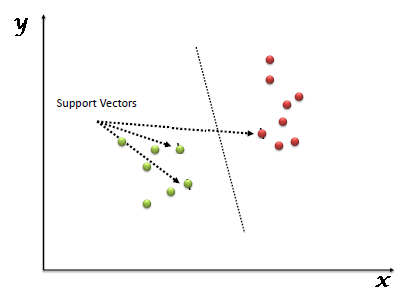
\includegraphics[width=0.7\linewidth]{media/media/image14.png}
\caption{Source: \cite{ray2017how_114} Hyperplane with support vectors.}
\label{fig:hyperplane-support-vectors}
\end{figure}

Finding such a hyperplane, see Figure 2.13, is an optimisation problem that involves
finding a function that has the most \emph{$\varepsilon$} deviation from the
obtained targets \emph{y\textsubscript{i}} for all the training data,
and at the same time is as flat as possible \cite{scholkopf2004tutorial_45}. The SVM classifier is a
frontier that best segregates the two classes in the hyper--plane.

If we take a linear function:

\begin{equation}
f(x)=\langle w,x\rangle + b,
\quad \text{with } w\in X,\; b\in \mathbb{R}.
\label{eq:svm-hyperplane}
\end{equation}


where \(\left\langle \ , \right\rangle\) is the dot product in X.
Flatness in the case of f(x) means that we seek a small \emph{w}. One
way to ensure this is the case is to minimise the norm, i.e.
\emph{\textbar\textbar w\textbar\textbar{}\textsuperscript{2} = \{w,
w\}}. In other words, we are looking for as small `\emph{w'} as possible
and we can convert this into an optimisation problem:
\begin{equation}
\begin{aligned}
\min_{w,b}\quad & \frac{1}{2}\,\lVert w\rVert^{2} \\
\text{s.t.}\quad
& y_i - \langle w, x_i\rangle - b \le \varepsilon, \\
& \langle w, x_i\rangle + b - y_i \le \varepsilon,
\qquad i=1,\ldots,M .
\end{aligned}
\label{eq:svr-epsilon-insensitive}
\end{equation}


The convex optimisation problem above implies that there is a function
\emph{f} that approaches all pairs of \emph{x\textsubscript{i},
y\textsubscript{i}} under the accepted constraint \emph{$\varepsilon$}.

Given a training set of instance--label pairs
\emph{(x\textsubscript{i},y\textsubscript{i}) i= 1,\ldots,n} where
\emph{x $\in$ R\textsuperscript{n}} and \emph{y $\in$
\{1,--1\}\textsuperscript{T}}, the SVM require the solution of the
following convex problem:

\begin{equation}
\begin{aligned}
\min_{w,b,\xi}\quad & \frac{1}{2}\,\lVert w\rVert^{2} + C\sum_{i=1}^{n}\xi_i \\
\text{s.t.}\quad
& y_i\bigl(\langle w,x_i\rangle + b\bigr) \ge 1-\xi_i,\qquad i=1,\ldots,n, \\
& \xi_i \ge 0,\qquad i=1,\ldots,n.
\end{aligned}
\label{eq:soft-margin-svm}
\end{equation}


where \emph{$\xi$\textsubscript{i}} are the slack variables introduced by
the method which measures the degree of misclassification of the data
\emph{X\textsubscript{i}}. If \emph{X\textsubscript{i}} is correctly
classified, then \emph{$\xi$\textsubscript{i}} = 0, otherwise
\emph{$\xi$\textsubscript{i}} \textgreater0. The larger the
\emph{$\xi$\textsubscript{i}} is, the more the SVM is penalized for
misclassifying \emph{X\textsubscript{i}}. \emph{w} is the normal vector
orthogonal to the hyperplane; \emph{b} is the offset of the hyperplane
from the origin along the normal vector \emph{w} and \emph{C
\textgreater{} 0} is the penalty/cost parameter of the error term. The
parameter \emph{C} controls the trade--off between minimizing the error
term and maximizing the margin. A larger value of \emph{C} means that
the SVM will be more penalized for misclassifications, and a smaller
value of \emph{C} means that the SVM will be more tolerant of
misclassifications. Different values of parameter \emph{C} are tested to
achieve the best results in the forecasting problem. This formulation is
for the soft margin SVM. The cost function includes a term that
penalizes misclassifications, while still trying to find a hyperplane
that separates the two classes as well as possible.

The soft margin SVM is a more flexible model than the hard margin SVM
which requires all the data points to be correctly classified. The soft
margin SVM is more robust to noise and outliers, can tolerate some
misclassifications and is a more flexible model than a hard margin SVM.

As Figure 2.14 below shows, only the points outside the drawn area have
impact to the cost. The points inside the drawn area are correctly
classified, and the points outside are misclassified. Deviations are
penalised linearly, which means the cost of misclassifying a point
increases linearly as the point moves further away from the decision
boundary.

\begin{figure}[htbp]
  \centering
  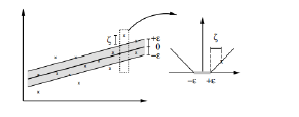
\includegraphics[width=0.9\linewidth]{media/media/image15.png}
  \caption{Source: \cite{ray2017how_114} Decision Boundary of Soft Margin SVM.}
  \label{fig:svm-soft-margin-boundary}
\end{figure}


Using the Lagrange multiplier to solve the convex optimisation problem
above we get the regression function:

\begin{equation}\label{eq:2.1.31}
y = f(x) = \sum_{i=1}^{M} \left(a_i - a_i^{*}\right)\,\langle x, x^{i}\rangle + b .
\end{equation}


where \emph{a\textsubscript{i,} a\textsuperscript{*} \textgreater0} are
the Lagrange multipliers that correspond to the support vectors.

If the dataset is not linear, SVR will not transform the data to a
high--dimensional feature space, but instead it uses the kernel trick
decision function, and the regression function becomes the following:

\begin{equation}\label{eq:2.1.32}
y = f(x) = \sum_{i=1}^{M} \left(a_i - a_i^{*}\right)\,k(x, x^{i}) + b .
\end{equation}


where \emph{k(x, x\textsuperscript{i})} is the kernel function and it
can be any function that is a dot ---- product transformed to a high
dimensional space.

The linear and radial kernel functions are applied where:

\begin{itemize}
\item
  Linear means the following:
\end{itemize}

\begin{equation}\label{eq:2.1.33}
k(x, x^{i}) = x^{\top} x^{i}.
\end{equation}


where \emph{k(x, x\textsuperscript{i})} is the kernel function and it
can be any function that is a dot ---- product transformed to a high
dimensional space.

\begin{itemize}
\item
  Radial Basis Function (RBF) means the following:
\end{itemize}

Radial basis function (RBF) kernel in SVM is a function used within
Support Vector Machines (and other kernel methods) to measure similarity
between two data points x and x'.

\begin{equation}\label{eq:2.1.34}
k(x, x^{i}) = \exp\!\left(-\frac{\|x - x^{i}\|^{2}}{2\sigma^{2}}\right).
\end{equation}


where \emph{$\sigma$} is the hyper--parameter which corresponds to the width of
the Gaussian kernel centred at \emph{x\textsuperscript{i}}. This kernel
is used by the SVM algorithm to handle nonlinear classification or
regression boundaries without explicitly mapping the data into a
higher--dimensional feature space (i.e., the kernel trick).

SVR often enjoys better performance than simple MLP Neural Networks. The
reasons for this being:

\begin{itemize}
\item
  Fewer hyperparameters. In general, SVM requires less grid searching to
  obtain a reasonably accurate model. SVMs with RBF kernels generally
  perform well. Unlike gradient problems with Neural Networks and local
  optima problem, SVM guarantees global optimum.
\item
  Overall, SVMs are good because the training algorithm is efficient and
  it has a regularisation parameter, which forces you to think about
  regularisation and overfitting.
\item
  In a classic Neural Network, the number of parameters is enormously
  high. For example, for vectors of the length 100 that must be
  classified into two classes, one hidden layer of the same size as an
  input layer will lead to more than 100,000 free parameters. One can
  imagine how badly the model can overfit and think how many training
  points the model will need to prevent that and how much time it will
  take to train it then.
\item
  Usually, one must be a real expert to choose the topology at a glance.
  That means that to get good results, data scientist should perform
  lots of experiments. That is why it's easier to use SVM and far harder
  to achieve similar results with NN.
\item
  Usually, NN results can vary unless random seeds and hyperparameters
  are controlled.
\end{itemize}

An RBF network is a type of artificial neural network commonly used for
function--approximation tasks. It typically consists of three layers: an
input layer, a hidden layer of radial basis function units, and an
output layer \cite{haykin1999neural_46}.

In the hidden layer, a Gaussian function is often used as the transfer
(activation) function. This allows the network to act as a universal
approximator with a relatively fast learning rate. RBF model training is
considered complete when it meets a specified error threshold (e.g.,
0.01) or when a fixed number of training iterations (e.g., 500) has
passed. For instance, one might choose an RBF network with 10 nodes in
its hidden layer.

Because of the Gaussian activation, the RBF network can converge more
quickly than some Multi--Layer Perceptrons (MLPs). Once training is
finished, both MLPs and RBF networks can then be tested under new
conditions. The agreement between model predictions and observed data is
compared, and the final model is selected based on whichever yields the
least error.

\hypertarget{volatility--forecasting--using--random--forest--regressor}{%
\section{\texorpdfstring{\textbf{VOLATILITY FORECASTING USING RANDOM
FOREST
REGRESSOR}}{VOLATILITY FORECASTING USING RANDOM FOREST REGRESSOR}}\label{volatility--forecasting--using--random--forest--regressor}}

A random forest regressor is a meta--estimator that fits several
regression trees on sub--samples of the dataset and uses averaging to
improve predictive accuracy and control over--fitting. The sub--sample
size is controlled with the \emph{max\_samples} parameter if
\emph{bootstrap = True (default),} otherwise the whole dataset is used
to build each tree. These sub--samples are created through a process
called bootstrap sampling, where each sub--sample is generated by
randomly selecting instances from the original dataset with replacement.

Random forests or random decision forests are an ensemble learning
method for classification, regression and other tasks that operates by
constructing a multitude of decision trees at training time. For
classification tasks, the output of the random forest is the one chosen
by most trees. For regression tasks, the mean or median prediction of
the individual trees is returned. Random decision forests correct for
decision trees' habit of overfitting to their training set. Random
forests generally perform better than decision trees, but their accuracy
is lower than gradient--enhanced trees. However, data characteristics can
affect their performance.

Taylor \cite{taylor1999quantile_47} proposed a Quantile Regression (QR) to forecast
financial time series volatility by estimating the conditional
probability distribution of multi--period asset returns. D. Pradeepkumar
\cite{pradeepkumar2017forecasting_48} presented a novel Particle Swam Optimization (PSO) trained
Quantile Regression Neural Network (PSOQRNN) to forecast volatility from
financial time series. The authors compared the effectiveness of PSOQRNN
with that of the traditional volatility time series forecasting models
i.e. GARCH, ANNs and MLP, General Regression Neural Network (GRNN),
Group Method of Data Handling (GMDH), Random Forest (RF) and two
Quantile Regression (QR) ---- based hybrids including Quantile Regression
Neural Network (QRNN) and Quantile Regression Random Forest (QRRF).
Their results indicate that the proposed PSOQRNN outperformed the other
models in terms of Mean Squared Error (MSE) in most of the cases.

Random Forest Regression is a supervised learning algorithm that uses
ensemble learning method for regression. Ensemble learning method is a
technique that combines predictions from multiple machine learning
algorithms to make a more accurate prediction than a single model - see Figure 2.15 below. 
Random Forest combines multiple decision trees into one model.

\begin{figure}[htbp]
  \centering
  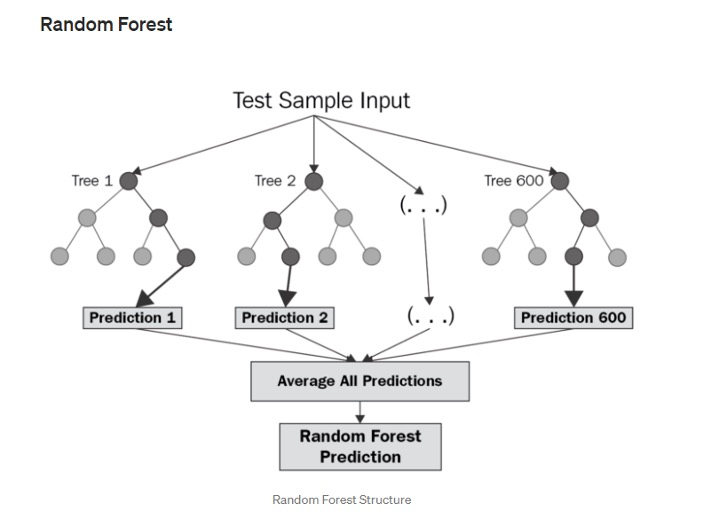
\includegraphics[width=5in,height=3.61111in,keepaspectratio]{media/media/image16.jpeg}
  \caption{Source: \cite{chakure2019random_115} RF.}
  \label{fig:RF}
\end{figure}

N\_estimators is the parameter that controls the number of trees in the
forest. Increasing the number of trees typically improves accuracy but
at the cost of increased computation time. Since Random Forest is an
ensemble method comprising of creating multiple decision trees, this
parameter is used to control the number of trees to be used in the
process.

In this thesis, the number of trees used is n\_estimator. As we know,
n\_estimator is one of the key parameters in Random Forest Regressor.
The input taken here is Volatility column of the dataset.

\hypertarget{forecasting--financial--time--series--volatility--using--arima--framework}{%
\section{\texorpdfstring{\textbf{FORECASTING FINANCIAL TIME SERIES
VOLATILITY USING ARIMA FRAMEWORK}
}{FORECASTING FINANCIAL TIME SERIES VOLATILITY USING ARIMA FRAMEWORK }}\label{forecasting--financial--time--series--volatility--using--arima--framework}}

A. Banerjee \cite{banerjee2020forecasting_49} used ARIMA (AutoRegressive Integrated Moving
Average) ARIMA model to forecast VVIX. ARIMA is a powerful statistical
method used to forecast time series data. It models the dependency
between an observation and a number of lagged observations
(autoregressive component, \emph{p}), the differences required to make
the series stationary (integrated component, \emph{d}), and the
dependency between an observation and a lagged forecast error (moving
average component, \emph{q}). Based on literature from Park \cite{park2015volatilityofvolatility_50},
they considered the VVIX as an indicator of `fat tail' risk i.e., the
risk of extreme events. They found ARIMA (1,0, 4) was the fittest model
to forecast future VVIX values.

This means the model includes one autoregressive term (\emph{p}=1), no
differencing (\emph{d}=0), and four moving average terms (\emph{q}=4).
The moving average component (\emph{q=4}) plays a crucial role in
adjusting predictions based on recent forecast errors. In financial time
series like VVIX, large deviations from predictions can occur due to
unexpected market news or geopolitical events. By using the last four
errors, the model smooths out these fluctuations, creating a more stable
forecast that aligns with observed behaviour. Furthermore, the absence
of differencing (\emph{d=0}) indicates that VVIX data is inherently
stationary, fluctuating around a mean level without long--term trends or
seasonality, which is typical for volatility indices.

The choice of ARIMA (1, 0, 4) reflects an optimisation process that
involved minimising information criteria AIC and BIC to achieve the best
balance between model fit and complexity. Higher--order models with
additional parameters might overfit the data, while simpler
configurations could fail to capture VVIX's nuanced short--term dynamics.
Banerjee's model thus provides an effective yet computationally
manageable approach to forecasting.

In validating the model, the study assessed its reliability using
residual diagnostics and metrics such as Mean Squared Error (MSE) and
Root Mean Squared Error (RMSE). These measures confirmed the model's
ability to accurately predict VVIX values while maintaining the
statistical assumptions of white noise residuals. By forecasting VVIX,
the ARIMA (1, 0, 4) model enables financial market participants to
anticipate extreme volatility periods, supporting more informed risk
management strategies. While ARIMA provides a robust baseline for
forecasting, it also highlights potential for hybrid approaches to
account for nonlinearities in financial time series data.

\begin{landscape}
\begin{figure}[p]
\centering 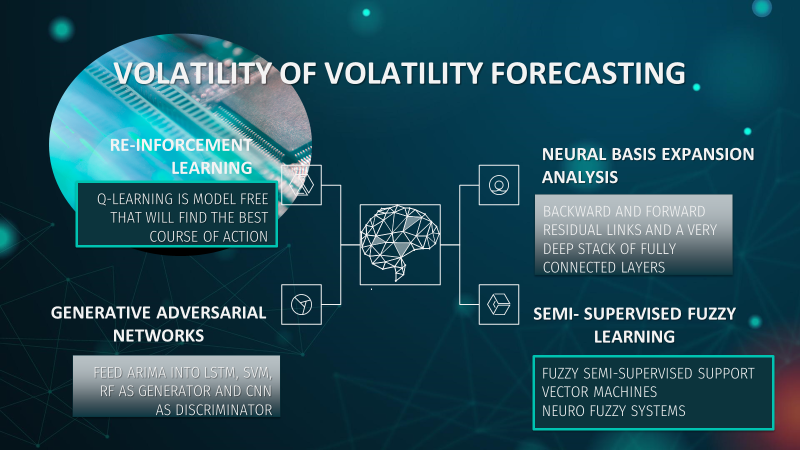
\includegraphics[width=\linewidth]{media/media/image17.png} \caption{ADVANCED MACHINE LEARNING MODELS}
\label{fig: ADVANCED MACHINE LEARNING MODELS}
\end{figure}
\end{landscape}



\hypertarget{neural--basis--expansion--nbeats}{%
\section{\texorpdfstring{\emph{\textbf{NEURAL BASIS EXPANSION
(NBEATS)}}}{NEURAL BASIS EXPANSION (NBEATS)}}\label{neural--basis--expansion--nbeats}}

Oreshkin et al., proposed a novel architecture for univariate time
series forecasting. They applied it to a variety of time series
forecasting problems using non--overlapping competition datasets: M4, M3
and Tourism. The results significantly outperformed traditional
econometric forecasting techniques \cite{oreshkin2019nbeats_51}.

N--BEATS is a novel deep learning architecture designed for interpretable
univariate time series forecasting. The focus is on solving the
univariate times series point forecasting problem using deep learning
architecture based on backward and forward residual links and a very
deep stack of fully connected layers. Although N--BEATS was initially
designed for univariate forecasting, extensions have been used for
multivariate time series forecasting by combining outputs from multiple
univariate models. The backcast link takes the historical data as input
and produces a representation of the past. In other words, it removes
the portion of the historical data that the block can approximate,
leaving the residual error for subsequent blocks to model. The forecast
link takes the representation of the past and produces a partial
forecast for future time steps. The architecture has several desirable
properties, being interpretable, applicable without modification to a
wide array of target domains, and fast to train.

The model consists of a sequence of stacks, each of which combine
multiple blocks. The blocks connect feedforward networks via forecast
and backcast links. A block ``removes the portion of the signal \ldots{}
it can approximate well'' \cite{oreshkin2019nbeats_51}. Then the block sets its focus on the
residual error, which the preceding blocks could not disentangle. This
residual error becomes the input for the subsequent blocks. Each block
generates a partial forecast, with its focus set on the local
characteristics of the time series. The stack aggregates partial
predictions on the blocks it consists of, and then passes the results on
to the next stack. The purpose of the stack is to identify non--local
patterns along the complete time axis by ``looking back.'' Each stack in
N--BEATS aggregates partial forecasts from its constituent blocks. This
hierarchical arrangement allows the model to progressively capture both
local characteristics (within blocks) and global patterns (across
stacks) along the time axis. Finally, the partial forecasts are
aggregated into an overall forecast at the model level.

N--BEATS takes as its hyperparameters:

\begin{enumerate}
\def\labelenumi{\roman{enumi}.}
\item
  The size of the input and output layers (constants INLEN and N\_FC)
  must be sufficient to assign a node for each feature in the source
  data. Each feature should have a corresponding node in the input and
  output layers. The length of the input segment should not be less than
  the order of seasonality, otherwise the learning process will have
  more difficulty combining the segments. For efficient memory usage,
  set them to a power of 2. For univariate time series, the size of the
  input layer corresponds to the length of the historical window, while
  the output layer represents the number of future time steps to
  forecast.
\item
  The number of~blocks in a stack~(BLOCKS).
\end{enumerate}

\begin{itemize}
\item
  N--beats consists of a sequence of stacks, each containing multiple
  blocks.
\item
  The number of blocks in a stack (BLOCKS) is a hyperparameter that
  determines the depth and complexity of the model.
\end{itemize}

\begin{enumerate}
\def\labelenumi{\roman{enumi}.}
\setcounter{enumi}{2}
\item
  The~width~of each fully connected~layer~in each block of a stack: its
  node count (LWIDTH).
\end{enumerate}

\begin{itemize}
\item
  The width of each fully connected layer in each block(LWIDTH) refers
  to the node count of these layers.
\item
  The width determines the capacity of the network to learn and
  represent complex patterns in the time series data.
\end{itemize}

The batch size determines the number of cases the model will process
before updating its matrix weights. To effectively align it with the
memory structure of our system, we set it to a power of 2. Very large
batch sizes can skew gradients down only in one direction, and the model
can get stuck at a sub--optimal minimum. Smaller batch sizes will cause
the gradient descent to bounce around in different directions and can
result in lower accuracy, but they also tend to prevent the model
from~overfitting. The most frequent recommendation is to choose an
initial batch size of 32. Since our dataset has a frequency of 24 hours
per day, we set the batch size to the following binary limit that can
handle 24--time steps: 32. The epochs tell the model the number of cycles
the exercise has to perform in each epoch, the model processes the
entire training set, performing one forward pass and one back pass.
Allowing for some oversimplification, the product of these
hyperparameters defines the tensor size of the model. Large parameter
values \hspace{0pt}\hspace{0pt}can cause it to reach the system's memory
limit and cause exponentially longer processing times. While small
parameter values \hspace{0pt}\hspace{0pt}may not be sufficient to
reflect complex patterns in the source data. Probabilistic forecasting
can be achieved in N--BEATS by incorporating quantile regression. This
technique allows the model to estimate not only a central forecast but
also uncertainty intervals, such as 10\%/90\% quantiles. This is an
option we can exercise in all deep forecasting models. The loss function
of a neural network can be constructed using~\emph{quantile loss
function.}~Then quantile regression will not only compute a central
forecast value at each time step, a point estimate, but will draw
uncertainty bands about it. Pairs of quantiles like 1\%/99\% or
10\%/90\% express the range over which the forecast value can vary,
above or below the central value.

\hypertarget{reinforcement--learning--rl}{%
\section{\texorpdfstring{\emph{\textbf{REINFORCEMENT LEARNING
(RL)}}}{REINFORCEMENT LEARNING (RL)}}\label{reinforcement--learning--rl}}

Reinforcement learning (RL) is a framework where an agent interacts with
its environment by taking actions, transitioning between states, and
receiving rewards. The agent aims to maximize cumulative rewards over
time by learning an optimal policy, often modelled as a Markov Decision
Process (MDP). A reinforcement learning agent can perceive and interpret
its environment, take actions, and learn through trial and error.
Reinforcement learning is one of the three fundamental models of machine
learning, along with supervised and unsupervised learning. Model--free RL
algorithms, such as Q--learning, do not require explicit knowledge of the
environment's dynamics (transition probabilities and reward functions).
This makes them suitable for financial markets, where the environment is
often unknown and non--stationary. Obviously, if we knew the model of
financial markets, we would just follow that model. This is what makes
forecasting financial data so difficult. We plan to implement Q--learning
in our approach. Q--learning updates the Q--value for each state--action
pair using the Bellman equation, which incorporates the immediate reward
and the estimated value of the next state. This iterative process
enables the agent to learn an optimal policy by balancing exploration
and exploitation. In Q--learning we will learn the value of taking an
action from a given state. Q--value is the expected return after taking
such action. We plan to utilise 'Rainbow,' an advanced deep
reinforcement learning algorithm that combines several enhancements to
the Deep Q--Network (DQN), including prioritised experience replay,
double Q--learning, duelling network architectures, and distributional
Q--learning. Reinforcement learning differs from supervised learning in
that it does not need to present labelled input/output pairs and does
not need to be explicitly corrected for suboptimal actions. Instead, the
focus is on finding a balance between exploration of uncharted territory
and exploitation of current knowledge \cite{moore1996reinforcement_52}.~Partially supervised RL
algorithms can combine the advantages of supervised and RL algorithms
\cite{pandian2018control_53}.

An environment in reinforcement learning is often modelled as a Markov
Decision Process (MDP) because many reinforcement learning algorithms in
this context use dynamic programming techniques.~It is defined by
states, actions, transition probabilities, and reward functions. The
Markov property ensures that the future state depends only on the
current state and action, simplifying the decision--making process. MDPs
form the theoretical foundation of many RL algorithms, enabling the
agent to learn policies that maximise cumulative rewards. The main
difference between classical dynamic programming methods and
reinforcement learning algorithms is that the latter do not assume
knowledge of an exact mathematical model of the MDP, and they target
large MDPs where exact methods become infeasible.

A Markov chain is a stochastic model, whereby the probabilities
connecting a sequence of partially random events is examined \cite{geyer1992practical_54}.
Markov series describe relationships between events in a sequence, which
is necessary for models used in financial analysis where underlying
trends in data must be observed. In the reinforcement model, the agent
is the Markovian decision maker and is responsible for trying to make
the optimal decision based on his understanding of the data. This
Agent's objective becomes a continuous process, where the Agent acts
upon its environment then evaluates the outcome of their action, then
takes this outcome into consideration in their next action. See Figure 2.17 below.

\begin{figure}[htbp]
\centering
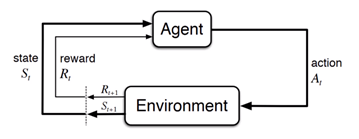
\includegraphics[width=3.73958in,height=1.44792in,keepaspectratio]{media/media/image18.png}
\caption{Source: \cite{andrew1998reinforcement_55} \emph{Reinforcement Learning}.}
\label{fig:reinforcement-learning}
\end{figure}

M. Taghian \cite{taghian2022learning_56} used a novel Deep Reinforcement Learning (DRL)
method to extract asset--specific trading rules from vast amounts of
historical data to increase the return and reduce risk of their
portfolio. DRL is implemented to learn the new trading rules for each
asset. The authors proposed a novel DRL model with various feature
extraction techniques. The proposed model outperformed the other
state--of--the--art models in learning single asset--specific trading rules.
W. Bao et al. \cite{w2017deep_57} combined transforming the data using wavelet
transforms (WT), stacked autoencoders (SAEs) and long--short term memory
(LSTM) for stock market forecasting. First, the time series were
decomposed by WT to eliminate the noise. Then, SAEs were applied to
generate a deep high--level feature for predicting the stock price and
lastly, the high--level de--noised features are fed into LSTM to forecast
the next day's closing price. Results showed that the proposed model
outperformed other similar models in both predicting accuracy and
profitability performance. M. Taghian et al. \cite{taghian2021reinforcement_58} employed a novel
encoder--decoder framework combined with DRL to learn single instrument
trading strategies from a long sequence of raw data of the instrument.
The model consisted of an encoder which is a neural structure
responsible for learning informative features from the input sequence
and a decoder which is DRL model responsible for learning profitable
strategies based on the features extracted by the encoder. The
parameters of the encoder and the decoder structures were learned
jointly which enabled the encoder to extract features specifically
tailored to the task of the decoder DRL. Jae Won Lee \cite{lee2001stock_59} presented
a method of calculating state values different from conventional
indicators in that they represent directly the expected cumulative
reward, the price rate of change, and not the auxiliary information for
making buying and selling decisions. While stock price prediction is not
strictly Markovian due to its dependence on external and long--term
factors, it can be approximated as a Markov process to enable
reinforcement learning models such as TD(0) and TD($\lambda$) to operate
effectively. TD($\lambda$) generalises TD(0) by introducing a parameter $\lambda$ that
weights immediate and future rewards, enabling the model to better
handle delayed returns------a critical feature for financial forecasting.
We plan to extend this method to other algorithms such as TD($\lambda$) where
our definition of reward will be different from Lee's paper. Nuno Horta
et al \cite{horta2018reinforcement_60} described a new system for short--term speculation in the
foreign exchange market based on RL. Neural Networks with three hidden
layers of ReLU neurons are trained as RL agents under Q--Learning
algorithm by an algorithm that consistently induces stable learning that
generalizes to out--of--sample data. This framework includes new state and
reward signals, and a method for more efficient use of available
historical tick data that provides training quality and testing
accuracy. Financial markets present unique challenges for reinforcement
learning compared to deterministic environments like Atari or Go. These
challenges include non--stationary data, where underlying market dynamics
change over time; partial observability, where not all relevant
variables are available to the agent; and high levels of noise in the
signals, which can obscure meaningful patterns. It was shown by the
authors that learning in the training dataset is stable and it is
apparent from several validation learning curves that the Q--network is
capable of finding relationships in financial data that translate to
out--of--sample decision making.

\hypertarget{a--generative--adversarial--network--gan}{%
\section{\texorpdfstring{\emph{\textbf{A GENERATIVE ADVERSARIAL
NETWORK
(GAN)}}}{A GENERATIVE ADVERSARIAL NETWORK (GAN)}}\label{a--generative--adversarial--network--gan}}

A~generative adversarial network~(GAN) is a class of~machine
learning~frameworks designed by~Ian Goodfellow~and his colleagues in
June 2014 \cite{goodfellow2014generative_61}.~Two~neural networks~compete in a~zero--sum game,
where one agent's gain is another agent's loss.

With a training set, this technique learns to generate new data with the
same statistics as the training set. For example, an image--trained GAN
can produce new images that appear realistic at least to a human
observer, with many realistic features. Though originally proposed as a
form of~generative model~for~unsupervised learning, GANs have also
proved useful for~semi--supervised learning,~fully~supervised
learning,~and~reinforcement learning.

The core idea of a GAN is based on the ``indirect`` training through the
discriminator, another neural network that can tell how much an input is
``realistic``, which itself is also being updated dynamically. This
basically means that the generator is not trained to minimize the
distance to a particular frame, but rather to fool the discriminator.
This enables the model to learn in an unsupervised manner. The generator
indirectly minimizes a divergence measure between the real and generated
data distributions, such as Jensen--Shannon divergence or Wasserstein
distance.

GANs are like~mimicry~in~evolutionary biology, with an~evolutionary arms
race~between both networks. To learn the generator's distribution
p\textsubscript{g} over data x, we define a prior on input noise
variables p\textsubscript{z}(z) then represent a mapping to data space
as G(z; $\Theta$\textsubscript{g}), where G is a differentiable function
represented by a multiplayer perceptron with parameters
$\Theta$\textsubscript{g}. We also define a second multilayer perceptron D (x;
$\Theta$\textsubscript{d}) that outputs a single scalar. D(x) represents
probability that x came from the data rather than p\textsubscript{g}. We
train Discriminator (D) to maximise the probability of assigning the
correct label to both training examples and samples from G.
Simultaneously we train G to minimise log(1 ---- D(G(z))):

So, in other words, D and G play the following two--player minimax game
with value function V(G, D) \cite{goodfellow2014generative_61}:

\begin{equation}\label{eq:2.1.35}
\min_{G}\max_{D} V(D,G)
= \mathbb{E}_{x\sim p_{\text{data}}(x)}\!\big[\log D(x)\big]
+ \mathbb{E}_{z\sim p_{z}(z)}\!\big[\log\!\big(1 - D(G(z))\big)\big].
\end{equation}

Kang Zhang et al \cite{zhanga2018stock_63} proposed a novel architecture of GAN with
Multi--Layer Perceptron (MLP) as the discriminator and LSTM as the
generator for forecasting the closing stock prices. The generator is
built by LSTMN to mine the data distribution of stocks from given data
and generate data in the same distributions, whereas the discriminator
designed MLP to discriminate between real and fake data. Their results
showed that the novel GAN structure gave promising results compared with
other models in machine learning and deep learning. HungChun Lin et al
\cite{lin2021stock_64} proposed stock price prediction model using GAN with Gated
Recurrent Units (GRU) used as a generator that inputs historical stock
price and generates future stock price and Convolutional Neural Network
(CNN) as a discriminator to discriminate between real and fake
distributions. Different to one step ahead forecasts only, the authors
used deep learning to make multi--step ahead predictions more accurately.
The authors also found that Wasserstein GAN performed better during
unexpected events like COVID whereas conventional GAN performed better
during normal times. They also showed that RNN--based GANs can become
unstable due to the sequential nature of RNNs, which complicates
gradient updates during adversarial training and requires careful tuning
of hyperparameters. The key is tune parameters in each layer to make the
whole model more accurate. Rainbow, an RL--based framework, has been
explored for hyperparameter optimisation in GANs, though its practical
implementation in adversarial networks remains experimental. Martin
Erdman et al \cite{erdmann2018generating_65} used adversarial network with the Wasserstein
distance to generate simulated detector data. The authors investigated
two variants of GANs for detector simulations. In both cases, the
transfer of probability distributions from one data set to another using
GAN training worked well using the Wasserstein distance in the loss
function. WGAN replaces the Jensen--Shannon divergence with the
Wasserstein distance, providing a more stable loss function that
alleviates vanishing gradient issues and improves training stability.
Instead of training a deep network with simulations that differ in
detail from data, simulations can be adapted to match data prior to
network training. With this method, authors showed that results are
better compared to training with the originally simulated traces.

\hypertarget{fuzzy--neural--network--fnns}{%
\section{\texorpdfstring{\emph{\textbf{FUZZY NEURAL NETWORK
(FNNS)}}
}{FUZZY NEURAL NETWORK (FNNS) }}\label{fuzzy--neural--network--fnns}}

``Fuzzy set is a class of objects with a continuum of grades of
membership. Such a set is characterized by a membership (characteristic)
function which assigns to each object a grade of membership ranging from
zero to one. Concepts of inclusion, union, intersection, complement,
relation, convexity, etc., are extended to such sets, and various
properties of these notions in the context of fuzzy sets are
established'' \cite{zadeh1965fuzzy_66}. Fuzzy neural networks (FNNs) for pattern
classification often use the backpropagation or C--cluster type learning
algorithms to learn the parameters of the fuzzy rules and membership
functions from the training data. However, such kinds of learning
algorithms usually cannot minimize training and testing errors
simultaneously and thus cannot reach a good classification performance
in the testing phase. To overcome this drawback, a support--vector--based
fuzzy neural network classification (SVFNNC) is proposed. The SVFNNC
leverages the robust classification capabilities of SVMs and the ability
of FNNs to model uncertainty through fuzzy logic. The learning algorithm
consists of two learning steps. In step 1, the fuzzy rules and
membership functions are generated using clustering principles, enabling
the system to model data uncertainty. In step 2, an adaptive fuzzy
kernel function enhances SVM performance by fine--tuning FNN parameters
for classification tasks. Deng et al \cite{deng2017deep_67} developed and tested a
system combining deep Neural Network with Direct Reinforcement learning
using fuzzy learning to summarise the market trend. The system was able
to select features from raw data and learn effectively using DL
mechanism. Fuzzy logic is particularly effective in financial markets
due to its ability to handle noisy and uncertain data, capturing subtle
patterns that may not be apparent with traditional machine learning
techniques.

\hypertarget{literature-review-conclusion}{%
\section{\texorpdfstring{\textbf{CONCLUSION}}{CONCLUSION}}\label{literature-review-conclusion}}

Despite decades of research and renewed attention following major market dislocations (e.g., the 2008 global financial crisis and the COVID-19 shock), the volatility forecasting literature remains characterised by \emph{plurality rather than consensus}: performance is strongly horizon- and regime-dependent, and simple benchmarks can remain surprisingly competitive relative to more elaborate specifications. This motivates the thesis to move beyond purely conditional-variance or purely data-driven approaches by explicitly targeting the \emph{fractal/long-memory structure} of volatility and integrating an \emph{uncertainty-aware} representation via fuzzy modelling within a fractional Brownian framework.

This chapter has reviewed a broad spectrum of volatility and volatility--of--volatility modelling approaches, ranging from classical econometric specifications to multifractal processes and modern machine learning. Across these strands, a consistent empirical message emerges: volatility is not well represented by memoryless Gaussian diffusion. Instead, volatility dynamics exhibit \emph{clustering}, \emph{heavy tails}, \emph{regime dependence}, and \emph{scale effects} that are naturally described through long--memory and (multi)fractal viewpoints. In this context, models such as mixed/fractional Brownian frameworks and multifractal constructions (e.g., MMAR/MSM) are motivated by their ability to encode persistence (or anti--persistence), time deformation (trading time), and heterogeneous activity across scales. By contrast, standard GARCH--type models capture conditional heteroskedasticity effectively at short horizons but struggle to simultaneously represent abrupt shifts and prolonged volatility cycles, while purely data--driven machine learning models often achieve strong predictive performance yet may under--represent long--range dependence and scale invariance unless these properties are explicitly engineered into the feature set and experimental design.

A second theme is that \emph{volatility of volatility} is central to modern volatility markets, but remains comparatively under--developed in the forecasting literature. While VIX has been extensively studied, the evidence base for VVIX forecasting is thinner and less systematic, particularly regarding approaches that integrate fractal/multifractal structure with state--of--the--art deep learning, reinforcement learning, or generative modelling. Moreover, even when advanced models are proposed, there is limited consensus on how to (i) robustly handle structural breaks and non--stationarity, (ii) ensure out--of--sample stability under changing market regimes, and (iii) quantify uncertainty in a way that is interpretable and decision--relevant for risk management.

These gaps motivate the direction of the thesis. First, rather than treating VVIX as a secondary quantity, the thesis elevates VVIX as the \emph{primary} object for understanding and forecasting the dynamics that drive implied volatility. This is consistent with the chapter’s core framing that volatility and its first derivative have fractal signatures, and that a scale--aware methodology is therefore required. Second, the thesis builds on the multifractal and fractional literature by developing a modelling pipeline that explicitly targets \emph{time--scale invariance}: fractal measures (e.g., Hurst exponent and related roughness diagnostics) are used not only as descriptive statistics but as structural inputs to model selection and forecasting. Third, the thesis introduces an uncertainty--aware extension through fuzzy modelling, allowing parameters and latent state descriptions to represent imprecision in a controlled mathematical form. In particular, the broader thesis framework aligns with recent developments that unify fractional drivers, fuzziness, and jump risk within a coherent stochastic setting (including risk--neutral considerations), thereby providing a principled bridge between fractal dynamics and uncertainty quantification. This is especially relevant because the literature indicates that fully formal treatments of fuzziness in the rough (non--semimartingale) regime remain limited, and careful construction is required to preserve mathematical consistency of inference and simulation across regimes. Finally, the thesis responds to the commonly noted need for stronger empirical substantiation of complex fractional/fuzzy frameworks by adopting a comparative, benchmark--driven evaluation strategy against established econometric baselines and modern machine learning models, with explicit attention to robustness and practical viability.

Chapter~3 now operationalises these objectives by detailing the datasets, pre--processing, stationarity and scaling diagnostics, and the full experimental design used to evaluate classical, multifractal, deep learning, and uncertainty--aware modelling approaches for VIX and VVIX.

\hypertarget{chapter--3------data--and--methodology}{%
\chapter{\texorpdfstring{\textbf{CHAPTER 3 -- DATA AND
METHODOLOGY}}{CHAPTER 3 -- DATA AND METHODOLOGY}}\label{chapter--3------data--and--methodology}}

This chapter details the data sources, pre--processing protocols, and the
complete experimental design used to conduct the empirical analysis in
this thesis. A transparent and replicable methodology is essential for
validating the findings and grounding the theoretical work in a robust
empirical foundation. We outline the process for daily and
high--frequency data acquisition and cleaning, the statistical tests for
data stationarity, the specific design for training and evaluating the
machine learning models, and the methodology for multifractal
simulations.

\hypertarget{smoothing--and--transforming--data}{%
\section{\texorpdfstring{\emph{\textbf{DATA ACQUISITION AND DESCRIPTION}}
}{DATA ACQUISITION AND DESCRIPTION }}\label{smoothing--and--transforming--data}}

To investigate the research questions, this study utilises two distinct datasets sourced from Kaggle and the Bloomberg Terminal. Each dataset was subjected to a preliminary inspection to assess its size, variable types, and data quality.

\hypertarget{daily--vix--index--data}{%
\subsection{Data Description and Quality Assessment}\label{daily--vix--index--data}}

The primary source for long-term historical volatility data is the "VIX Daily" dataset obtained from Kaggle (Yahoo finance). This dataset provides a daily time series of the CBOE Volatility Index (VIX) [P1], [P4]. Kaggle is a platform hosting datasets
and competitions related to machine learning and data science. The
primary dataset was collected from the following link -
\url{https://www.kaggle.com/jonathanbesomi/cboe--volatility--index--vix}.
\begin{itemize}
    \item \text{Dimensions and Scope:} The dataset covers the period from January 2, 1990, to April 20, 2022, containing approximately 8,143 observations.

    \item \text{Variables:} The raw file (\texttt{VIX\_daily.v1.csv}) consists of two primary columns:
    \begin{itemize}
        \item \text{Date:} Recorded in DD/MM/YYYY format.
        \item \text{Last Price:} The daily closing value of the VIX index.
    \end{itemize}

    \item \text{Quality Assessment:}
    \begin{itemize}
        \item \text{Completeness:} The dataset is highly structured with no obvious formatting errors in the timestamp index.
        \item \text{Stationarity:} Preliminary visual inspection confirms the data exhibits mean--reverting behaviour typical of volatility indices, though it contains extreme outliers corresponding to market crises (e.g., 2008, 2020) which act as ``shocks'' in the time series.
    \end{itemize}
\end{itemize}

To capture high-frequency dynamics and the "volatility of volatility," a second dataset was extracted directly from the Bloomberg Professional Terminal. This dataset includes both daily and 30-minute interval data for the VIX and the CBOE VIX of VIX Index (VVIX).

\begin{itemize}
    \item \text{Dimensions and Scope:}
    \begin{itemize}
        \item \text{Daily Data:} Covers VIX and VVIX closing prices. The VVIX daily series begins on January 3, 2007 resulting in a shorter historical range compared to the VIX.
        The raw VVIX daily file contains 3,997 observations.
        \item \text{Intraday Data:} Includes 30--minute snapshots covering the recent period from \text{August 2021 to April 2022}. The intraday VIX dataset contains \text{4,702 observations}, while the corresponding VVIX dataset contains \text{2,542 observations}.
    \end{itemize}

    \item \text{Variables:}
    \begin{itemize}
        \item \text{Date:} Timestamp including date and time (e.g., \texttt{2022-04-20 09:15:00}).
        \item \text{Last Price:} The index value at the specific interval.
        \item \text{\#Ticks:} The number of ticks recorded in the interval (measure of activity).
        \item \text{SMAVG (15):} A 15--period Simple Moving Average included in the raw export.
    \end{itemize}

    \item \text{Quality Issues and Pre--processing:}
    \begin{itemize}
        \item \text{Formatting Artifacts:} The raw Bloomberg exports (\texttt{VVIX AND VIX DATA.xlsx}) contain leading empty columns (e.g., \texttt{,,Date,Last Price}) and metadata headers that required removal before analysis.
        \item \text{Missing Values:} Specific instances of missing data were identified. For example, the \texttt{VVIX DAILY.csv} file shows a single null value for \text{Last Price} on \text{2022-04-20} at the very end of the series.
        \item \text{Timestamp Alignment:} The 30--minute intervals required alignment to ensure that VIX and VVIX observations corresponded to the exact same timestamps, necessitating the removal of unmatched rows during the data cleaning phase.
    \end{itemize}
\end{itemize}

During the initial inspection, a small subset of data points was identified containing a recorded price or volume of zero. For the VIX and VVIX indices, a value of zero is theoretically inconsistent with the underlying pricing models (e.g., variance swaps), as it implies a complete absence of market volatility. Consequently, these values were classified as data feed anomalies or reporting errors rather than genuine market signals.

Justification for Deletion vs. Imputation- the decision was made to remove these artifacts rather than attempt imputation (such as forward-filling or mean substitution) for two primary reasons:
\begin{enumerate}
    \item \text{Preservation of Ground Truth:} Since the VIX is the target variable for prediction, imputing missing values would effectively train the models on synthetic data, potentially introducing bias.
    \item \text{Sample Integrity:} The instances of zero or missing values were extremely rare, constituting approximately 0.025\% of the total dataset. Given this negligible proportion, deletion preserves the statistical integrity of the time series without reducing statistical power.
\end{enumerate}

Analysis was
conducted using Python programming via Google Colaboratory. 

To ensure stationarity and work with a more statistically stable series,
we focused on the daily log returns of the VIX rather than the raw VIX
index [P4]. Returns were calculated using the formula:

\begin{equation}\label{eq:3.1.1}
\mathrm{Return}(t)
= \ln\!\left(\frac{\mathrm{VIX}(t)}{\mathrm{VIX}(t-1)}\right).
\end{equation}


Then calculate volatility of VIX by, first, calculating its standard
deviation and then multiplying by square root of 252 trading days in a
year. This transformation assumes that returns are independently and
identically distributed (i.i.d.), even though clustering and jumps are
known characteristics of volatility. The reason for this transformation
and data manipulation is to convert the standard deviation of percentage
changes in VIX for a sample of days into the standard deviation of
percentage changes annualised. Hence, we take daily returns as log of
(VIX2/VIX1), then we calculate standard deviation of this log return and
multiply by the square root of 252 trading days in a year.

\textbf{Theoretical Derivation based on Hull and CBOE} 

The VIX formula is derived from the pricing of a variance swap. As shown by Hull \cite{hull2006options_116}, the fair delivery price for a variance swap can be replicated by a static portfolio of out--of--the--money (OTM) calls and puts weighted by the inverse squared strike price ($1/K^2$).

The theoretical value of the annualized variance is given by the replication of the ``Log Contract'':
\begin{equation}
    E[\bar{\sigma}^2] = \frac{2}{T} \left( rT - \left( \frac{S_0}{S_*} e^{rT} - 1 \right) - \ln \frac{S_0}{S_*} \right)
\end{equation}

By discretizing this integral across available option strikes, we obtain the standard operational formula used by the CBOE:

\begin{equation}\label{eq:3.1.2}
\sigma^{2} = \frac{2}{T}\sum_{i=1}^{N}\frac{\Delta K_i}{K_i^{2}}\,e^{R T}\,Q(K_i) - \frac{1}{T}\left(\frac{F}{K_0}-1\right)^{2}.
\end{equation}

\footnote{K. Demeterfi, E. Derman, M. Kamal and J. Zou,
\emph{More Than You Ever Wanted to Know About Volatility Swaps (But Less Than Can Be Said)},
Goldman Sachs Quantitative Strategies Research Notes, March 1999.}

\begin{quote}
VIX = $\sigma$ * 100
\end{quote}

T = Time to expiration

F = Forward index level derived from index option prices

Ko = First strike (the strike price is the price at which an option
holder can exercise the option) below the forward index level, F

K\textsubscript{i} = Strike price of i\textsubscript{th} out of the
money option; a call if K\textsubscript{i} \textgreater{}
K\textsubscript{0} and a put if K\textsubscript{i} \textless{}
K\textsubscript{0}; both put and call if K\textsubscript{i} =
K\textsubscript{0} (put and call options are two types of derivatives
that give the holder the right to sell or buy the underlying asset at
the strike price on or before the expiration date in case of American
option or on expiration date if the option is European).

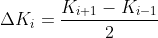
\includegraphics[width=1.64583in,height=0.39583in]{media/media/image31.png}

R = Risk--free interest rate to expiration

Q(Ki) = The midpoint of the bid--ask spread for each option with strike
Ki.

\emph{\uline{Proof:}}

\emph{If return of the day i is r\textsubscript{i}, r\textsubscript{i}
is independently and identically distributed across i time periods and
the standard deviation of r\textsubscript{i,} is}
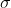
\includegraphics[width=0.125in]{media/media/image32.png}\emph{,
then variance of n day returns, r\textsubscript{1} + r\textsubscript{2}
+ \ldots r\textsubscript{n}, equals expected value of
\{(r\textsubscript{1} + r\textsubscript{2} + \ldots r\textsubscript{n})
---- E{[}r\textsubscript{1} + r\textsubscript{2} +
\ldots r\textsubscript{n}{]}\}\textsuperscript{2}. The expression can be
expanded to n square terms of the form (r\textsubscript{i} ----
E{[}r\textsubscript{i}{]})\textsuperscript{2} each of which has expected
value of}
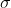
\includegraphics[width=0.125in]{media/media/image32.png}\emph{\textsuperscript{2}
and n(n--1)/2 cross terms of the form (r\textsubscript{i} ----
E{[}r\textsubscript{i}{]})( (r\textsubscript{j} ----
E{[}r\textsubscript{j}{]}), each of which has expected value of 0
because of independence assumption. So variance of r\textsubscript{1} +
r\textsubscript{2} + \ldots r\textsubscript{n} equals
n}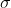
\includegraphics[width=0.125in]{media/media/image32.png}\emph{\textsuperscript{2}
and standard deviation equals}
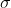
\includegraphics[width=0.125in]{media/media/image32.png}
\emph{$\sqrt{}$n. With n=252 trading days, the standard deviation equals to}
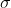
\includegraphics[width=0.125in]{media/media/image32.png}
\emph{$\sqrt{}$252.}

This transformation helps to normalise the data and is a standard
procedure in the financial time--series analysis. All models, unless
otherwise specified, were trained on this transformed series.

\hypertarget{stationarity--test--of--the--data}{%
\section{\texorpdfstring{\emph{\textbf{STATIONARITY TEST OF THE
DATA}}}{STATIONARITY TEST OF THE DATA}}\label{stationarity--test--of--the--data}}

As detailed in the literature review, stationarity is essential for time
series analysis. We formally tested for the presence of a unit root in
the daily log--return series of the VIX using the Augmented Dickey--Fuller
(ADF) test. Suppose a random variable S(t) is stationary. This behaviour
can be more formally described by the following stochastic differential
equation (SDE).

\begin{equation}\label{eq:3.1.3}
\mathrm{d}S_t
= \theta\bigl(\mu - S_t\bigr)\,\mathrm{d}t
+ \sigma\,\mathrm{d}W_t .
\end{equation}


where, W(t) is a Wiener process (Brownian motion) at time t, the rate of
reversion $\theta$ to mean, the equilibrium of mean value of the process $\mu$ and
its volatility $\sigma$. According to this SDE, the variation of price at
\emph{t+1} is proportional to the difference between the price at time t
and the mean. So, the price change is more likely to be positive or
negative if the price is smaller or greater than the mean.

\hypertarget{hypothesis--test--and--stationarity--test}{%
\subsection{\texorpdfstring{\emph{HYPOTHESIS TEST AND STATIONARITY
TEST}
}{HYPOTHESIS TEST AND STATIONARITY TEST }}\label{hypothesis--test--and--stationarity--test}}

A set of data is stated to be stationary if the average value, variance,
and autocorrelation of the series are constant. In other words, the
statistical properties do not change over time. The stationarity test is
conducted to ensure that the return data have been stationary. The stationarity test of return data is
conducted by using ADF (Augmented Dickey Fuller) Test. ADF test aims to
find out whether the return data still contain the unit root or not. A
unit root is a value that causes the series to trend over time. If the
return data does not contain the unit root, it means that the data is
stationary. Then it can be used in the further estimation processes.
However, if the ADF test results show that the return data still
contains the unit root (not stationary) then the differencing process of
the data should be conducted until its condition becomes stationary
\cite{livieris2021smoothing_25}. Differencing is a process of subtracting the previous value
from the current value. This process removes the trend from the series
and makes it stationary.

The ADF test is conducted using the hypothesis test as follows:

\emph{Ho : $\gamma$ = 1, there are unit roots and non--stationary data}

\emph{H1: stationary data}

If the ADF test statistic is smaller than the critical value or
possessing the probability which is smaller than 5\%, this means that
the data does not contain the unit roots anymore, so it is stationary.
If the data is not stationary yet, then it is necessary to conduct the
differencing process of the data until the ADF test value is smaller
than its critical value.

\hypertarget{stationarity--concepts}{%
\subsection{\texorpdfstring{\emph{STATIONARITY CONCEPTS}
}{STATIONARITY CONCEPTS }}\label{stationarity--concepts}}

As cited before, modelling financial time series is a complex task, due
to some properties of financial data. Stock prices have the following
stylised facts \cite{francq2010garch_69}:

\begin{enumerate}
\def\labelenumi{\roman{enumi}.}
\item
  The price series are usually non--stationary and close to a random
  walk. A random walk assumes that price changes are random, and they
  wander unpredictably.
\item
  This model makes impossible to predict future patterns. Therefore,
  stationarity is a crucial element in time series analysis.
\end{enumerate}

There are two different definitions of stationarity. Firstly, ``a
process ($X$$t$) is said to be strictly stationary if the vectors ($X$1, . . .
, $X$$k$)' and ($X$1+$h$, . . . , $X$$k$+$h$)' have the same joint distribution, for
any $k$ $\in$ $\mathbb{N}$ and any $h$ $\in$ $\mathbb{Z}$'' \cite{francq2010garch_69}.

In other words, a process is strictly stationary if its unconditional
joint probability distribution does not change when shifted in time, and
so do parameters, such as mean and variance. Another weaker definition
of stationarity is known as second--order stationarity, and it requires
only the first moment and the autocovariance not to vary with the time.
The second moment, or the variance, should only be finite.

In statistics and econometrics, an augmented Dickey----Fuller test (ADF)
tests the null hypothesis that a unit root is present in a time series
sample. The alternative hypothesis is different depending on which
version of the test is used but is usually stationarity or
trend--stationarity. It is an augmented version of the Dickey----Fuller
test for a larger and more complicated set of time series models that is
normally used.

The augmented Dickey----Fuller (ADF) statistic \cite{elliott1996efficient_70} used in the test,
is a negative number. The more negative it is, the stronger the
rejection of the hypothesis that there is a unit root at some level of
confidence.

Testing procedure:

The testing procedure for the ADF test is the same as for the
Dickey----Fuller test but it is applied to the following model:

\begin{equation}\label{eq:3.1.4}
\Delta Y_t
= \alpha + \beta t + \gamma Y_{t-1}
+ \delta_{1}\Delta Y_{t-1} + \cdots + \delta_{p-1}\Delta Y_{t-p+1}
+ \varepsilon_t .
\end{equation}


where $\alpha$ is a constant, $\beta$ is the coefficient on a time trend and $\rho$ is the
lag order of the autoregressive process. Imposing the constraints $\alpha$ = 0
and $\beta$ = 0 corresponds to modelling a random walk and using the
constraint $\beta$ = 0 corresponds to modelling a random walk with a drift.
Consequently, there are three main versions of the test, analogous to
the ones discussed on Dickey----Fuller test.

By including lags of the order p, the ADF formulation allows for
higher--order autoregressive processes. This means that the lag length p
must be determined when applying the test. One possible approach is to
test down from high orders and examine the t--values on coefficients. An
alternative approach is to examine information criteria such as the
Akaike information criterion, Bayesian information criterion or the
Hannan----Quinn information criterion.

\hypertarget{application--and--results}{%
\subsubsection{APPLICATION AND RESULTS}\label{application--and--results}}

The ADF test was performed using the adfuller() function from Python
statsmodels library. Appendix A1 provides the full code and outputs for
reference. The Augmented Dickey--Fuller (ADF) test yielded a test statistic of $-6.71$, which is significantly lower than the $1\%$ critical value of $-3.43$. Furthermore, the $p$-value of $3.66 \times 10^{-9}$ provides overwhelming evidence to reject the null hypothesis of a unit root. Consequently, the time series is confirmed to be \text{stationary}, satisfying the prerequisite conditions for the proposed forecasting models.

\hypertarget{experimental--design--for--machine--learning--models}{%
\section{\texorpdfstring{\emph{\textbf{EXPERIMENTAL DESIGN FOR
MACHINE LEARNING MODELS}}
}{EXPERIMENTAL DESIGN FOR MACHINE LEARNING MODELS }}\label{experimental--design--for--machine--learning--models}}

\hypertarget{lstm--architecture}{%
\subsection{\texorpdfstring{\emph{LSTM ARCHITECTURE}
}{LSTM ARCHITECTURE }}\label{lstm--architecture}}

We give a brief overview of LSTM architecture here. This section is
related to section 3.5.3 where we present results from various deep
neural network models. LSTM is a particular type of deep neural network
developed by Hochreiter and Schmidhuber \cite{hochreiter1997long_35}. By inheriting the
benefits from the recurrent neural network (RNN), LSTM has shown great
power to model sequential data, like time series. Compared to vanilla
RNN, LSTM uses gates to control information flows through the sequence
so that it can be capable of learning long--term dependencies and solving
the vanishing gradient problem.

At a high--level LSTM is like an RNN cell. Here is the internal
functioning of the LSTM network. The LSTM consists of three parts, as
shown in the Figure below and each part performs an individual function
\cite{saxena2021introduction_36}.

\begin{figure}[htbp]
\centering
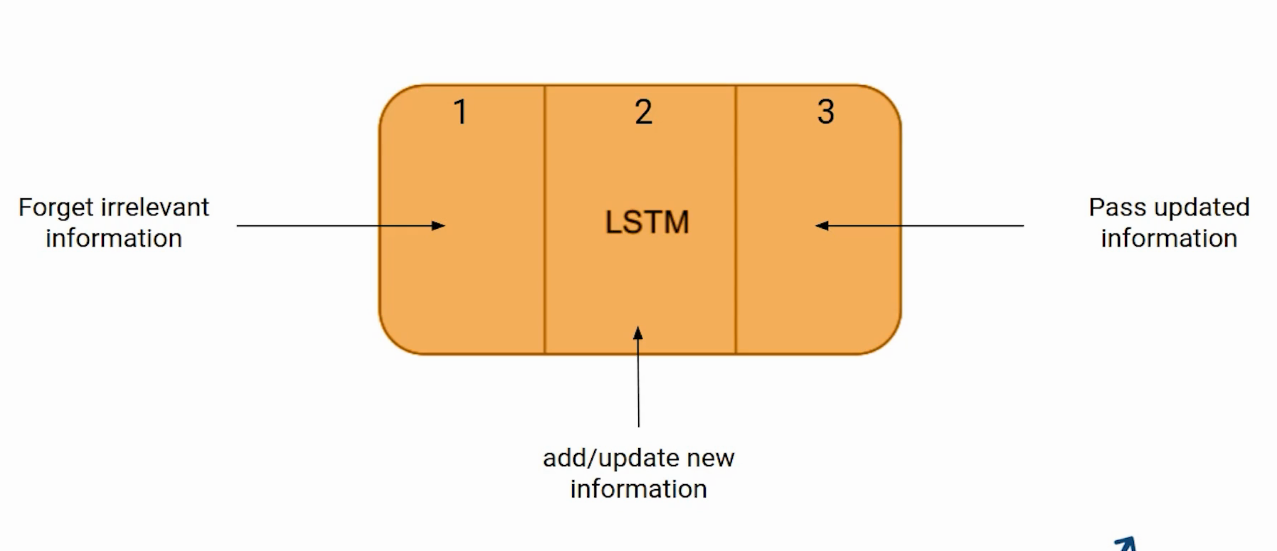
\includegraphics[width=0.85\linewidth]{media/media/image10.png}
\caption{Source: \cite{saxena2021introduction_36} LSTM cell.}
\label{fig:lstm-cell}
\end{figure}


The first part chooses whether the information coming from the previous
timestamp is to be remembered or is irrelevant and can be forgotten. In
the second part, the cell tries to learn new information from the input
to this cell. In the third part, the cell passes the updated information
from the current timestamp to the next timestamp \cite{agarwal2021nextwordpredictionusinglstm_37} .

These three parts of an LSTM cell are known as gates. The first part is
called Forget gate, the second part is known as the Input gate and the
last one is the Output gate.

The Figure below shows the typical architecture of LSTM. Like vanilla RNN,
inputs are imported into the model at each time step, and outputs can be
given at each time step. LSTM uses memory block to take place of neuron
in RNN. A memory block is composed of a memory cell, an input gate, a
forget gate, and an output gate. We can use vector formulas to describe
LSTM, as follows \cite{jia2021forecasting_28}:

\begin{itemize}
\item \textbf{Input gate:}
  \begin{equation}
  i_t = \sigma\!\left(W_{ix} x_t + W_{ih} h_{t-1} + b_i\right).
  \label{eq:lstm-input-gate}
  \end{equation}
\end{itemize}


\begin{itemize}
\item \textbf{Forget gate:}
  \begin{equation}
  f_t = \sigma\!\left(W_{fx} x_t + W_{fh} h_{t-1} + b_f\right).
  \label{eq:lstm-forget-gate}
  \end{equation}
\end{itemize}

\begin{itemize}

\item \textbf{Output gate:}
  \begin{equation}
  o_t = \sigma\!\left(W_{ox} x_t + W_{oh} h_{t-1} + b_o\right).
  \label{eq:lstm-output-gate}
  \end{equation}

\item \textbf{Candidate cell state:}
  \begin{equation}
  \widetilde{c}_t = \tanh\!\left(W_{cx} x_t + W_{ch} h_{t-1} + b_c\right).
  \label{eq:lstm-candidate-cell}
  \end{equation}

\item \textbf{Cell state:}
  \begin{equation}
  c_t = f_t \odot c_{t-1} + i_t \odot \widetilde{c}_t.
  \label{eq:lstm-cell-state}
  \end{equation}

\item \textbf{Hidden state:}
  \begin{equation}
  h_t = o_t \odot \tanh(c_t).
  \label{eq:lstm-hidden-state}
  \end{equation}

\end{itemize}

where:

\begin{itemize}
\item
  \emph{X\textsubscript{t}}~is the input at time~\emph{t}
\item
  \emph{H\textsubscript{t--1}} is the hidden state at time~\emph{t}-1
\item
  \emph{C\textsubscript{t}}~is the cell state at time~\emph{t}
\item
  \emph{i\textsubscript{t}}~is the input gate at time~\emph{t}
\item
  \emph{f\textsubscript{t}}\hspace{0pt}~is the forget gate at
  time~\emph{t}
\item
  \emph{o\textsubscript{t}}\hspace{0pt}~is the output gate at
  time~\emph{t}
\item
  \(\widetilde{c}\)\emph{\textsubscript{t}}~is the candidate cell state
  at time~\emph{t} that is used to store information in an LSTM cell
\item
  \emph{W}~are the weight matrices
\item
  \emph{b}~are the bias vectors
\item
  \emph{$\sigma$}~is the activation function with sigmoid function being
  popular
\item
  tanh~is the hyperbolic tangent function
\item
  $\nabla$ denotes pointwise multiplication
\end{itemize}

\begin{figure}[htbp]
\centering
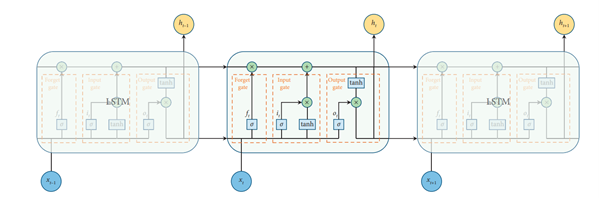
\includegraphics[width=0.95\linewidth]{media/media/image11.png}
\caption{Source: \cite{jia2021forecasting_28} LSTM architecture.}
\label{fig:lstm-architecture}
\end{figure}


We use a likelihood--based loss function when training our DNN and LSTM
models. The likelihood function is defined as the probability of
observing the actual return series given the model's predictions and
maximises the likelihood of observing the actual returns given the
predicted volatilities. If r\textsubscript{t} is the return series that
we observe from time 1 to time T and $\sigma$\textsubscript{t} is the
volatility that our models forecast at the same time step, we can
calculate the sample likelihood under the assumption of normal
distribution.

\begin{equation}
L(\{r_t\}_{t=1}^{T}\mid \{\sigma_t\}_{t=1}^{T})
= \prod_{t=1}^{T} \frac{1}{\sqrt{2\pi}\,\sigma_t}
\exp\!\left(-\frac{r_t^{2}}{2\sigma_t^{2}}\right).
\label{eq:likelihood-normal}
\end{equation}


Since the likelihood functions involves multiplying many probabilities
together, it is often more convenient to work with the logarithm of the
likelihood. Taking the logarithm transforms the product into a sum
simplifying the calculations. So, after taking logs of both sides we
have the log--likelihood functions \cite{jia2021forecasting_28}:

\begin{equation}
\log L(\{r_t\}_{t=1}^{T}\mid \{\sigma_t\}_{t=1}^{T})
= \sum_{t=1}^{T}\left(
-\frac{1}{2}\log(2\pi) - \log \sigma_t - \frac{r_t^{2}}{2\sigma_t^{2}}
\right).
\label{eq:loglikelihood-normal}
\end{equation}




The log--likelihood function should be maximized through optimization,
while the deep learning models are always trained by minimizing their
loss function. So, we need to use the negative log likelihood to be the
loss function in deep learning models. To further reduce the
computational cost of deep learning models, we use a simplified function
as the loss function of our DNN and LSTM models:

\begin{equation}
\mathrm{Loss} = \sum_{t=1}^{T}\left(2\log \sigma_t + \frac{r_t^{2}}{\sigma_t^{2}}\right).
\label{eq:loss-sigma}
\end{equation}


\begin{figure}[htbp]
\centering
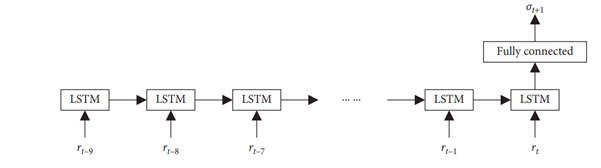
\includegraphics[width=0.95\linewidth]{media/media/image12.png}
\caption{Source: \cite{jia2021forecasting_28} LSTM with fully connected layer.}
\label{fig:lstm-fc}
\end{figure}

LSTM model combines LSTM with a fully connected layer in the last time
step. Its architecture is shown in the Figure above.

\hypertarget{gradient--vanishing--in--lstm}{%
\subsection{\texorpdfstring{\emph{GRADIENT VANISHING IN
LSTM}}{GRADIENT VANISHING IN LSTM}}\label{gradient--vanishing--in--lstm}}

Same as in RNNs, LSTM outputs a prediction vector h(k). The knowledge
encoded in the state vector c(t) captures the long--term dependencies and
the relations in the sequential data. The gradient descent is computed
to update the network parameters over T time steps. The vanishing
gradient problem occurs when the gradients in a neural network diminish
exponentially as they are backpropagated through layers and time steps.

\begin{figure}[htbp]
\centering
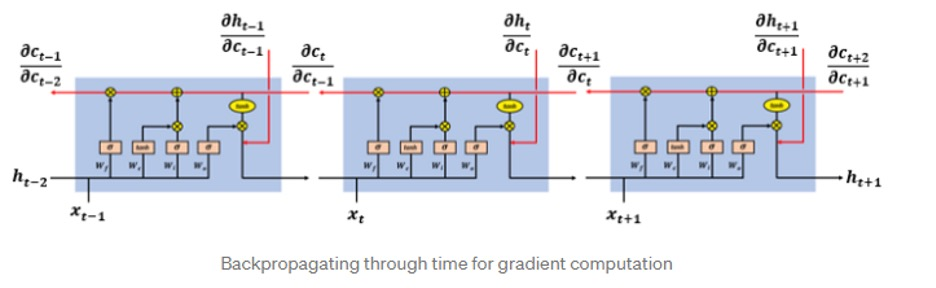
\includegraphics[width=0.95\linewidth]{media/media/image13.jpeg}
\caption{Source: \cite{jia2021forecasting_28} Gradient vanishing in LSTM.}
\label{fig:fig-2-13}
\end{figure}


The error term gradient is given by the same partial derivative as in
RNNs and the gradient of the error for time step k has the same form
given by variation of Taylor rule.

Backpropagation through time (BPTT) in RNN use gradients that are
calculated recursively from the final time step(T) to the initial time
step (t=1). The gradient at each step is obtained by multiplying the
gradient from the next time step with the derivative of the activation
function.

\begin{equation}
\delta_t = \delta_{t+1}\,\frac{\partial f(z_{t+1})}{\partial z_{t+1}}.
\label{eq:backprop-delta}
\end{equation}


$\delta$\textsubscript{t}\hspace{0pt} represents the gradient at time step t,
and f(z\textsubscript{t}) is the activation function applied to the
weighted sum z\textsubscript{t} at time step t. When calculating the
gradients through multiple time steps, the gradients are multiplied at
each time step due to the chain rule of differentiation. This leads to
an exponential decay of gradients as they are backpropagated to earlier
time steps. The following product causes the gradients to vanish:

\begin{equation}
\Delta W = \prod_{t=1}^{T}\frac{\partial f(z_t)}{\partial z_t}.
\label{eq:grad-product}
\end{equation}


\(\mathrm{\Delta}W\) represents the accumulated gradient term that is
multiplied at each time step.

Unlike traditional RNNs, LSTMs utilise a memory cell (c) and various
gates (input, forget and output gates) to control the flow of
information and prevent the vanishing gradient problem. The additive
property of the cell state gradients enables the network to update the
parameter in such a way that the different sub gradients do not
necessarily agree and behave in a similar manner making it less likely
that the functions converge to zero. In other words, LSTM allows for
better balancing and manipulation of gradient values during
backpropagation. This property along with the presence of the forget
gate, makes it less likely for the gradients to vanish. The forget gate
in an LSTM allows the network to control the gradients at each time step
and decide which information should be retained or forgotten. It helps
prevent the vanishing gradient problem by enabling the model to update
the parameters in a way that preserves important information.

\hypertarget{experimental--methodology}{%
\subsection{\texorpdfstring{\emph{EXPERIMENTAL METHODOLOGY}
}{EXPERIMENTAL METHODOLOGY }}\label{experimental--methodology}}

To ensure a robust and fair comparison of the machine learning models discussed in Chapter 2, a standardised experimental design was implemented.

\text{Train--Test Split Protocol:}
Given the computational intensity of the deep learning architectures (specifically the GAN and N--BEATS ensembles), a chronological hold--out validation strategy was employed. The daily VIX time series (1990--2022) was split chronologically to prevent lookahead bias:
\begin{itemize}
    \item \text{Training Set (70\%--80\%):} The initial majority of the dataset was used to train the models and capture long--term historical volatility regimes.
    \item \text{Test Set (20\%--30\%):} The final segment of the data was held out purely for out--of--sample evaluation.
\end{itemize}

\text{Feature Engineering:}
The input features ($X$) were engineered differently depending on the model architecture's specific requirements:

\begin{enumerate}
    \def\labelenumi{\roman{enumi}.}
    \item \text{N--BEATS Input:} For the N--BEATS model, a univariate lookback window approach was used. The model was fed a sequence of lagged log--returns (e.g., a 7--day window) to forecast the subsequent step ($t+1$).
    \item \text{GAN/CNN Input:} For the GAN and CNN models, a novel image--based encoding was applied. Sequential segments of 100 days were reshaped into $10 \times 10$ grids and subsequently padded to $32 \times 32$ matrices. This transformation allowed the use of 2D Convolutional layers to detect spatial patterns within the time--series data.
\end{enumerate}

\text{Hyperparameter Selection:}
Optimal hyperparameters were selected through a combination of grid search and literature--derived baselines:

\begin{itemize}
    \item \text{LSTM:} The LSTM model architecture consisted of 2 LSTM layers with 50 hidden units each, followed by a Dropout layer (rate 0.2) to mitigate overfitting. The model was optimized using Adam ($lr=0.001$) by minimizing the Mean Absolute Error (MAE).

    \item \text{N--BEATS:} To establish a rigorous baseline, the N--BEATS architecture adopted the optimal configuration recommended in the original literature \cite{oreshkin2019nbeats_51}. The generic architecture utilised a stack depth of 30, with 4 layers per block and a layer width of 512 units, trained over 5,000 epochs to ensure convergence.

    \item \text{GAN:} The Generative Adversarial Network was designed with a specialized architecture to handle the image--encoded time series. The Generator utilised Dense layers upsampled via Conv2DTranspose, while the Discriminator employed a 2D Convolutional Neural Network (Conv2D) to distinguish between real and synthetic volatility patterns. Training utilised the Adam optimiser with a learning rate of 0.0002 and $\beta_1=0.5$.
\end{itemize}

\textbf{Performance Evaluation:}
The 93.3\% accuracy metric associated with the GAN model refers strictly to the internal discriminator's ability to classify real versus generated data samples during training. It is not a forecasting metric. The true predictive performance of the hybrid framework is evaluated via the MAE and MAPE scores of the downstream regressors (SVM and Random Forest) that utilise the GAN--generated synthetic features for final prediction.
\hypertarget{methodology--of--generating--multifractal--simulations}{%
\section{\texorpdfstring{\emph{\textbf{METHODOLOGY OF GENERATING
MULTIFRACTAL
SIMULATIONS}}}{METHODOLOGY OF GENERATING MULTIFRACTAL SIMULATIONS}}\label{methodology--of--generating--multifractal--simulations}}

We will simulate approximately 30 years of data which should capture at
least 4 different economic cycles ---- 1990s boom and bust, 2000s housing
boom and bust, 2010s blockchain and cryptocurrency boom and bust and
COVID. This should give us the best chance to measure realistic
parameters.

\hypertarget{definition--of--a--multifractal--stochastic--process}{%
\subsection{Definition of a multifractal stochastic
process:}\label{definition--of--a--multifractal--stochastic--process}}

A stochastic process \emph{X(t)} is defined as multifractal if it has
stationary increments, and satisfies:

\begin{equation}\label{eq:3.1.5}
\mathbb{E}\bigl[|X(t)|^{q}\bigr]
= c(q)\,t^{\tau(q)+1},
\qquad \forall\, t\in T,\; q\in Q .
\end{equation}

where \emph{T} and \emph{Q} are intervals on the real line and have positive lengths.

In this formulation, $c(q)$ represents a deterministic, moment--dependent prefactor that is independent of the time scale $t$. The function $\tau(q)$ is the \text{multifractal scaling exponent}, which characterizes the scaling behaviour of the process. The non--linearity of $\tau(q)$ with respect to $q$ is the defining condition for multifractality; a linear $\tau(q)$ would imply a monofractal process such as fractional Brownian motion.

Now we choose some values of \emph{q} (raw statistical moments) which
will be used for our empirical estimations. \cite{mandelbrot1997multifractal_13} used 99 values of
\emph{q} between 0.01 and 30 to estimate \emph{$\tau$(q)}. Next step is to
find the partition function by splitting the data into \emph{N}
non--overlapping subintervals, whose length \emph{$\Delta$t} is less than our
total time \emph{T}:

\begin{equation}\label{eq:3.1.6}
S_{q}(T,\Delta t)
= \sum_{i=0}^{N-1} \Bigl| X\bigl((i+1)\Delta t\bigr) - X\bigl(i\Delta t\bigr) \Bigr|^{q}.
\end{equation}


where \emph{N = T/$\Delta$t} is the total number of time increments for that
increment size. The partition function is the sum of the absolute values
of all increments of price change, raised to some given power q which is
a raw statistical moment for every size of time increment \emph{$\Delta$t.}

The time increments \emph{$\Delta$t} are the independent variable that we
manipulate (x--axis), and the partition function \emph{S\textsubscript{q}
(t, $\Delta$t)} is the dependent variable. This function is computed several
times over for different values of \emph{q}. Then we estimate the
scaling function $\tau$(q) by running OLS linear regression on the different
lines of the graph for different values of q \cite{calvet1997large_71}.

\begin{equation}\label{eq:3.1.7}
\ln\!\Big(\mathbb{E}\big[S_q(T,\Delta t)\big]\Big)
= \widehat{\tau}(q)\,\ln(\Delta t) + \widehat{c}(q)\,\ln(T).
\end{equation}


We run OLS regression on the partition function curve for each q. The
gradient of the straight line is the value of $\tau$(q) for that value of
\emph{q}. Through all the different OLSs, we will have many different
values for $\tau$(q) and the intercept \emph{c(q)} for different values of
\emph{q.}

Next, we will use non--linear regression to estimate non--linear curve
$\tau$(q) that goes through all the estimated values as closely as possible.
Next, we find the Hurst exponent \emph{H}. Using the estimated scaling
function $\tau$(q) and the following formula, we solve for H. This is derived
in \cite{mandelbrot1997multifractal_13}.

\begin{equation}\label{eq:3.1.8}
\tau_X\!\left(\frac{1}{H}\right)=0 .
\end{equation}

\begin{equation}\label{eq:3.1.9}
\therefore\quad \widehat{H}
= \frac{1}{\widehat{\tau}_X^{-1}(0)} .
\end{equation}

We find hurst exponent taking the inverse of the estimated scaling
function. Then we estimate the multifractal spectrum f(a) by performing
a Legendre transform on $\tau$(q). The Legendre transform is defined as a
technique that is used to convert functions of one quantity such as
position, pressure, or temperature into functions of the conjugate
quantity i.e., momentum, volume, entropy, respectively. In Mechanics,
there are two common approaches to describing motion ---- the Lagrangian
and the Hamiltonian. The Legendre transform is a technique that is used
to convert a Lagrangian function \emph{L (x, dx/dt, t)} which describes
a particle's velocity to a Hamiltonian function \emph{H (x, dL/(dx/dt),
t)} which describes its momentum. The function is the following:

\begin{equation}\label{eq:3.1.9}
H(p)=\sup_{x\in\mathbb{R}}\bigl\{p\,x - f(x)\bigr\}.
\end{equation}


where \emph{p = df(x)/dx} and \emph{sup} is the supremum function. The
supremum of a subset \emph{S} of a partially ordered set \emph{T} is the
least element in T that is greater than or equal to all elements of
\emph{S} if such an element exists. If the transform has a negative
sign, then instead of supremum we use infimum. The scaling function
should be concave, so we can define the multifractal spectrum of the
price process as:

\begin{equation}\label{eq:3.1.10}
\widehat{f}(\alpha)
= \inf_{q\in Q}\left\{\, q\,\alpha - \widehat{\tau}(q) \,\right\} + D .
\end{equation}

where inf refers to infimum. Infimum of a subset \emph{S} of a partially
ordered set \emph{T} is the greatest element in \emph{T} that is less
than or equal to all elements of \emph{S} if such an element exists.
Multifractal analysis aims to describe the singularity structure of a
dataset, which reflects the varying degrees of irregularity,
concentration of values, and scaling properties across different scales.
Singularities are points in the data where certain properties deviate
significantly from the expected regular behaviour. In financial time
series, these singularities could correspond to extreme events, crashes
or volatile periods. The multifractal spectrum characterises the scaling
exponents that quantify the local regularity or singularity at various
points within the dataset. These scaling exponents correspond to the
Hölder exponent (\emph{$\alpha$}), which describe the local scaling properties
of the data. High \emph{$\alpha$} values show regularity, while low $\alpha$ values
indicate singularity. Hölder exponent should not be confused with Hurst
exponent or Hausdorff dimension. These are related concepts but not the
same. Hölder exponents are used in multifractal analysis to characterise
the local scaling properties of a dataset. They indicate how the
regularity or singularity of a function varies at different points
within the data. The Hölder exponent $\alpha$ quantifies the rate of decay or
growth of the function's oscillations. 
In the context of multifractal analysis, $\alpha$ can vary across different
points, allowing for the characterisation of complex and irregular
datasets. The multifractal spectrum $\tau$(q) (sometimes also known as mass
exponent or scaling function) is related to the singularity spectrum
\emph{f($\alpha$)} through Legendre transform which is used to obtain $\tau$(q) from
\emph{f($\alpha$)} and vice versa. The transformation ensures that $\tau$(q) is a
concave function of \emph{q}, and \emph{f($\alpha$)} is its convex conjugate.
Concavity of the infimum operator is related to the multifractal scaling
properties and reflects the existence of different scaling behaviours at
various points within the dataset. Using the estimated multifractal
spectrum \emph{f(a)}, we can find the most probable H\"older exponent.

\begin{equation}\label{eq:3.1.11}
\widehat{\alpha}_0
= \widehat{f}^{-1}\!\left(\max_{\alpha}\widehat{f}(\alpha)\right).
\end{equation}

\emph{$\alpha$\textsubscript{0}} is the value of the H\"older exponent $\alpha$ for
which \emph{f($\alpha$\textsubscript{0}) = 1}. This should also be the maximum
value of the multifractal spectrum. If the data is multifractal, then it
has different H\"older exponents at different timepoints and
\emph{$\alpha$\textsubscript{0}} is the most commonly occurring exponent in the
data. Using the estimated values for \emph{H} and
\emph{$\alpha$\textsubscript{0}}, estimate the log--normal distribution
parameters for the multiplicative cascade ---- \emph{$\lambda$} and
\emph{$\sigma$\textsuperscript{2}}. The MMAR involves generating a
multiplicative cascade, whose masses are drawn from a continuous
probability distribution. The most common distribution used for these
cascades is the lognormal distribution with a mean \emph{$\lambda$} and a
variance \emph{$\sigma$\textsuperscript{2}}. \cite{mandelbrot1997multifractal_13} showed that these two
parameters are determined using H and $\alpha$\textsubscript{0}:

\begin{equation}\label{eq:3.1.12}
\widehat{\lambda}=\frac{\widehat{\alpha}_0}{\widehat{H}} .
\end{equation}

\begin{equation}\label{eq:3.1.13}
\widehat{\sigma^{2}}
=\frac{2\bigl(\widehat{\lambda}-1\bigr)}{\ln(b)} .
\end{equation}


We will use these two estimators to generate randomly distributed
Multipliers \emph{M\textsubscript{i}} to construct multifractal cascades
for the MMAR simulation. First, we choose the number of b--adic intervals
into which we will divide our time series at every step \emph{k}. So, at
every step \emph{k}, there should be \emph{b\textsuperscript{k}}
intervals in total. For example, if we choose the number of intervals as
2, then we have 1 interval at step zero; 2 intervals at step one; 4 at
step two and so on. Then choose some masses \emph{m\textsubscript{0}}
and \emph{m\textsubscript{1}.} The height of the graph for that interval
is the mass of the interval will be multiplied by the allocated mass
\emph{m\textsubscript{i}}. This would give us a simple cascade but if we
were to continue this process, we would get a graph with a series of
bars that look like scaled versions of each other. We need to introduce
randomness into the system so instead of having static mass allocations,
give them some probabilities of occurrence. Our mass allocations have
been mutually exclusive so if one side had \emph{m\textsubscript{0}}
then the other side had \emph{m\textsubscript{1}} and
\emph{m\textsubscript{0} + m\textsubscript{1} = 1}. Since the mass is
conserved as in laws of physics, such multiplicative cascade is called
conservative. The mass of each interval, which can be interpreted as the
probability mass, is redistributed such that the total always sums to 1.
However, if the mass allocations are independent of each other, this
would mean that their sum does not have to add up to 1 each time but the
expected sum of the distribution should be one. In other words, the
total weight of all masses on average should add to one. In fact, we
don't even need to have discrete probabilities or multipliers.

We can draw them from a continuous probability distribution. We can
replace our discrete multipliers with some random multipliers draw from
a distribution of our choice. The expected sum of the multipliers should
equal to one. This second type of multiplicative cascade is called a
canonical cascade, and it is the most used type in simulating MMAR model
and the one we will be using as well. The mass of each interval in
canonical cascade can vary independently, and while the sum might not
always be 1 in every specific instance, the expected sum over a large
number of instances or iterations is 1. This maintains the overall
conservation of mass (or probability mass) in a statistical sense. We
will also use binomial cascade meaning we will split each interval into
two i.e. b = 2.

From \cite{mandelbrot1997multifractal_13}, we get that:
\begin{equation}\label{eq:3.1.13}
V=-\log_{b} M \sim \mathcal{N}\!\left(\widehat{\lambda},\,\widehat{\sigma}^{2}\right).
\end{equation}

\begin{equation}\label{eq:3.1.14}
\mathbb{E}[M]
=\mathbb{E}\!\left[b^{-V}\right]
=\mathbb{E}\!\left[\exp\!\left(-V\ln b\right)\right]
=\exp\!\left(-\widehat{\lambda}\ln b + \frac{1}{2}\widehat{\sigma}^{2}(\ln b)^{2}\right)
=\frac{1}{b}.
\end{equation}

where \emph{V \textasciitilde{} N ($\lambda$,
$\sigma$\textsuperscript{2}\textsubscript{})} and as we established before in
3.5.9:

\[\widehat{\lambda} = \frac{\widehat{\alpha_{0}}}{\widehat{H}}\]

\[\widehat{\sigma^{2}} = \ \frac{2(\widehat{\lambda} - 1)}{\ln\lbrack b\rbrack}\]

The trading time cumulative distribution function (CDF) \emph{$\theta$(t)} is
the main component of MMAR and requires both high kurtosis and
volatility clustering to generate our simulated returns. To compute CDF
we will compute the cumulative sum of the cascade from time 0 to the end
of time T for each value of \emph{t}.

\begin{equation}\label{eq:3.1.14}
\theta(t)=F_{\mu}(t)=\sum_{i=0}^{t}\mu(i), \qquad t\in\mathbb{Z}_{\ge 0}.
\end{equation}

Fractional Brownian Motion is the other component of MMAR model. This is
the component that allows us to simulate random walks with Hurst
component other than 0.5.

B\textsubscript{H}(t) is a stochastic process characterized by the
following equation:

\begin{equation}\label{eq:3.1.15}
\begin{aligned}
B_H(t)
&=\frac{1}{\Gamma\!\left(H+\tfrac12\right)}
\Biggl[
\int_{-\infty}^{0}\Bigl((t-s)^{H-\tfrac12}-(-s)^{H-\tfrac12}\Bigr)\,\mathrm{d}B(s) \\
&\qquad\qquad +\int_{0}^{t}(t-s)^{H-\tfrac12}\,\mathrm{d}B(s)
\Biggr],\qquad t>0 .
\end{aligned}
\end{equation}


where:

\(\Gamma(z)\) represents the Euler Gamma function
\(\int_{- \infty}^{0}{\left\lbrack x^{z - 1}e^{- x} \right\rbrack dx}\)\emph{;}

\emph{H} represents the Hurst exponent, \emph{0 \textless{} H
\textless{} 1;}

\emph{B(s)} represents a typical stochastic Brownian motion with \emph{H
= 0.5;}

\emph{t} represents time.

These equations are used to simulate a random process with H $\neq$ 0.5.
Imagine that we have a white noise process, which we can think of as a
river of constantly fluctuating white noise. We want to integrate this
white noise process to obtain a process with a Hurst exponent other than
0.5. We can do this by building a dam across the river. The dam will
smooth out the white noise process, and the Hurst exponent of the
resulting process will depend on the height of the dam. The Wiener
integral is the mathematical equivalent of building a dam across a river
of white noise. The Hurst exponent of the resulting process will depend
on the parameters of the Wiener integral \cite{mandelbrot1977fractal_72}. Simulating fBm
requires setting the length of the fBm process. \cite{mandelbrot1997multifractal_13} has not said
anything of their fBm settings. We would manually adjust the simulated
data until the median standard deviation of returns was approximately
equal to that of real data.

The last step is to merge the trading time CDF with the fBm for
simulation of overall returns X(t). Wengert \cite{wengert2010mmar} offered MMAR code for
users of MATLAB software which we adjusted for Python when constructing
multiplicative cascade.

The methodology for generating multifractal simulations can be
summarised as follows. Estimate the Hurst exponent and the multifractal
spectrum \emph{f(a)}. The latter describes the distribution of the
fluctuations of the time series. So, we find the four empirical
parameters \emph{H, $\alpha$, $\lambda$, $\sigma$\textsuperscript{2}} by calculating the
partition function \emph{S\textsubscript{q}(T, $\Delta$t)}, the scaling
function $\tau$(q), and the multiplicative spectrum \emph{f(a)}. Then we
generate a lognormal multiplicative cascade. This is a random process
that is used to generate multifractal data. It is created by repeatedly
dividing a time series into smaller and smaller intervals and then
assigning random multipliers to each interval. The multipliers are drawn
from a lognormal distribution, which means they have a long right tail.
This ensures that the cascade has a high degree of variability. Next, we
convert the lognormal multiplicative cascade into a cumulative
distribution function (CDF). This function maps each possible value of a
random variable. CDF can be computed using the following simplified
mapping:
\(CDF(x)\  = \ \exp( - {|(\ln(x)\  - \ \lambda)|}^{2}\ /\ (2\sigma^{2})).\)
In other words, we simulate two random processes which are used as the
two components of the MMAR i) trading time function \emph{$\Theta$(t}) made by
converting a lognormal multiplicative cascade into a cumulative
distribution and ii) fBm which is like a random walk but the changes do
not have to be independent. fBm is a random process that is used to
model long term trends in a time series. It is created by adding
together a series of independent random walks, each of which has a Hurst
exponent of \emph{H}. Then we plug trading time into fBm so we can
interpret the compound process as simulation of price growth over time
\emph{X\textsubscript{t} = B\textsubscript{H}{[}$\Theta$(t){]}}. In other
words, we combine the CDF of the lognormal multiplicative cascade with
the fBm process. The result is a time series that has both long term
trends and short--term fluctuations.

The pseudo--code in Appendix A2 provides a simplified implementation of
this process. Achieving a complete implementation is an area of ongoing
work and constitutes a significant part of our planned future
developments.

\hypertarget{long--range--dependence--and--the--rescaled--range}{%
\subsection{LONG--RANGE DEPENDENCE AND THE RESCALED
RANGE}\label{long--range--dependence--and--the--rescaled--range}}

Mandelbrot used the Rescaled Range (R/S) test statistic to test for long
range dependence. The R/S statistic is the range of partial sums of
deviations of a series from its mean divided by the standard deviation.
Mandelbrot showed that R/S statistic led to superior results when
compared to analysis of autocorrelations and variance ratios. The R/S
statistic is obtained using the following method. Consider the time
series of length n:

\begin{equation}
\{x_j\}_{j=1}^{n} = \{x_1, x_2, \ldots, x_n\}.
\label{eq:sequence-ch3}
\end{equation}

The partial sum of \emph{k} deviation from the mean is given by:
\begin{equation}
\Pi_{k} \equiv \sum_{j=1}^{k}\left(x_{j}-\overline{x}_{n}\right)
= (x_{1}-\overline{x}_{n}) + (x_{2}-\overline{x}_{n}) + \cdots + (x_{k}-\overline{x}_{n}).
\label{eq:Pi_k-ch3}
\end{equation}


The R/S statistic is proportional to the difference between the maximum
and the minimum of such sums where \emph{k} $\epsilon$ {[}1, n{]}:

\begin{equation}
\frac{R}{S}(n)=\frac{1}{\sigma(n)}
\left[\max_{1\le k\le n}\Pi_k-\min_{1\le k\le n}\Pi_k\right].
\label{eq:RS_n-ch3}
\end{equation}

The denominator \emph{$\sigma$(n)} is the maximum likelihood standard deviation
estimator. The rescaled range and the number \emph{n} of observations
have the following relation:

\begin{equation}
\frac{R}{S} \propto n^{H}.
\label{eq:RS_scaling-ch3}
\end{equation}


where \emph{H} is the Hurst exponent. This relationship was observed
empirically by Hurst in his analysis of river flows. He found that the
range of cumulative deviations (rescaled by standard deviation)
exhibited self--similar behaviour across time scales. This observation is
now generalised to time series with long memory and fractal properties.
After taking logarithms of both sides in the equation above, we obtain the
relation between the rescaled range and the number of observations
\emph{n}:

\begin{equation}
\frac{R}{S} \approx A + B n^{H}
\;\Rightarrow\;
\log\!\left(\frac{R}{S}\right) \approx C + H \log n .
\label{eq:RS_log_linear-ch3}
\end{equation}


So, one can estimate the value of \emph{H} from the log--log plot as the
slope of the line. This is a standard procedure for identifying
long--term dependencies in time series.

In the next diagrams, we illustrate how the Hurst coefficient changes
with different assets, time frames and lags. The \emph{'lag1}' and
'\emph{lag2}' variables define the range of time lags we considered for
the analysis. For each time lag in the range, we calculated
'\emph{tau}', which represents the standard deviation of the differenced
time series. Specifically, '\emph{tau}' was obtained by computing the
standard deviation of the differences between two portions of the time
series data at each lag. This provided insight into how variability
changed as the time lag increased and was essential for estimating the
Hurst exponent, which characterises the long--term memory of the time
series. Next, we performed a linear regression analysis on the
logarithms of \emph{'lags}' and '\emph{tau}' using the '\emph{polyfit}'
function. The result, stored in '\emph{m}' corresponds to the slope of
the log--log plot. Finally, we used the slope from the linear regression
to calculate the Hurst exponent \emph{H}, which quantifies the
persistence or mean--reverting nature of the time series.

Figures 3.1--3.2 show long term time series of S\&P exhibits strong
persistent behaviour (\emph{H}=0.64) and short--term S\&P 500 is strongly
mean reverting (\emph{H} = 0.25). Stock prices rarely display
mean--reversion behaviour long--term as asset prices tend to follow random
walk and trend up with inflation over long time horizons. In contrast,
Figures 3.3--3.4 show that volatility is more mean reverting long term
and has more persistent behaviour but still mean reverting in the
short--term. It is quite intuitive as volatility tends to be within one
standard deviation long term but can become unbounded in the short term.
We can see it through bursts of volatility during crisis and subsequent
subsiding as it returns to its average corridor of one standard
deviation.

\begin{landscape}
\begin{figure}[p]
\centering
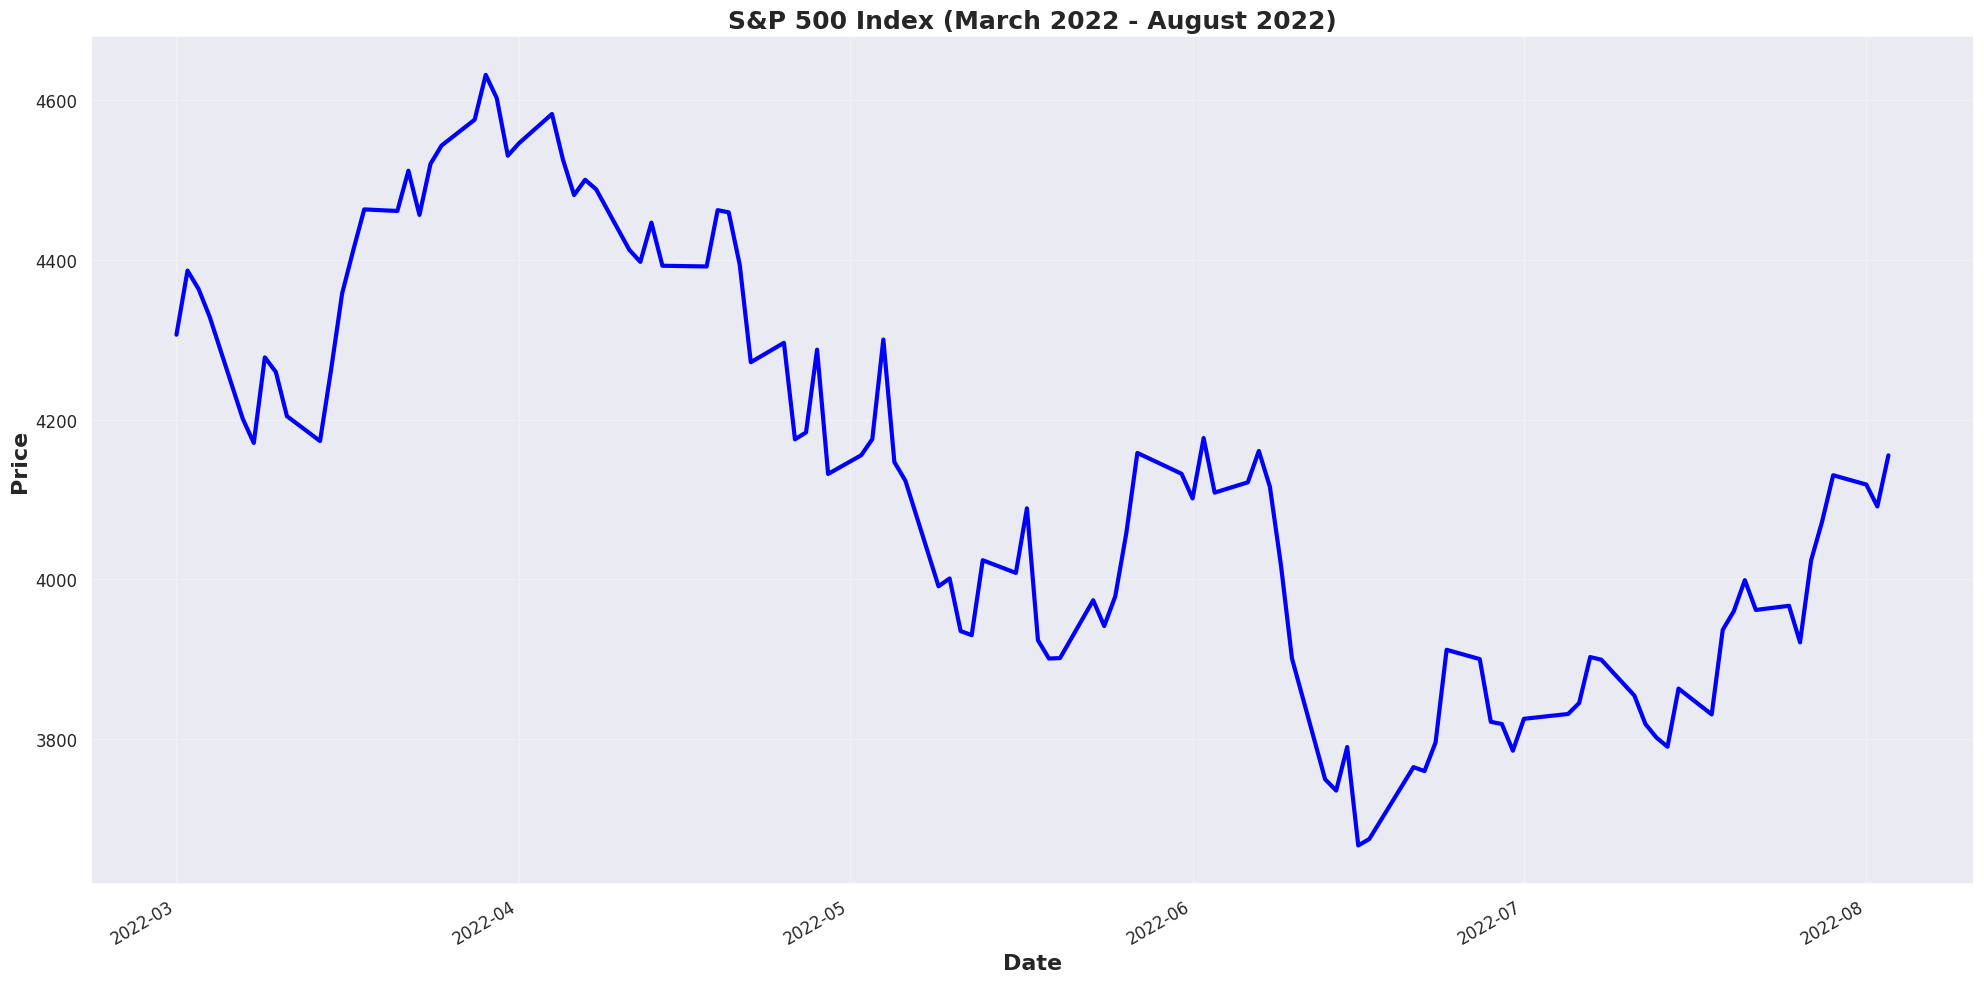
\includegraphics[width=\linewidth]{media/media/image5.png}
\caption{Time series: S\&P500 Hurst = 0.399, Lag 1, Lag 2 = 2, 20 Time: 3/1/2022 --- 4/8/2022.}
\label{fig:sp500-hurst-ch3}
\end{figure}
\end{landscape}

\begin{landscape}
\begin{figure}[p]
\centering
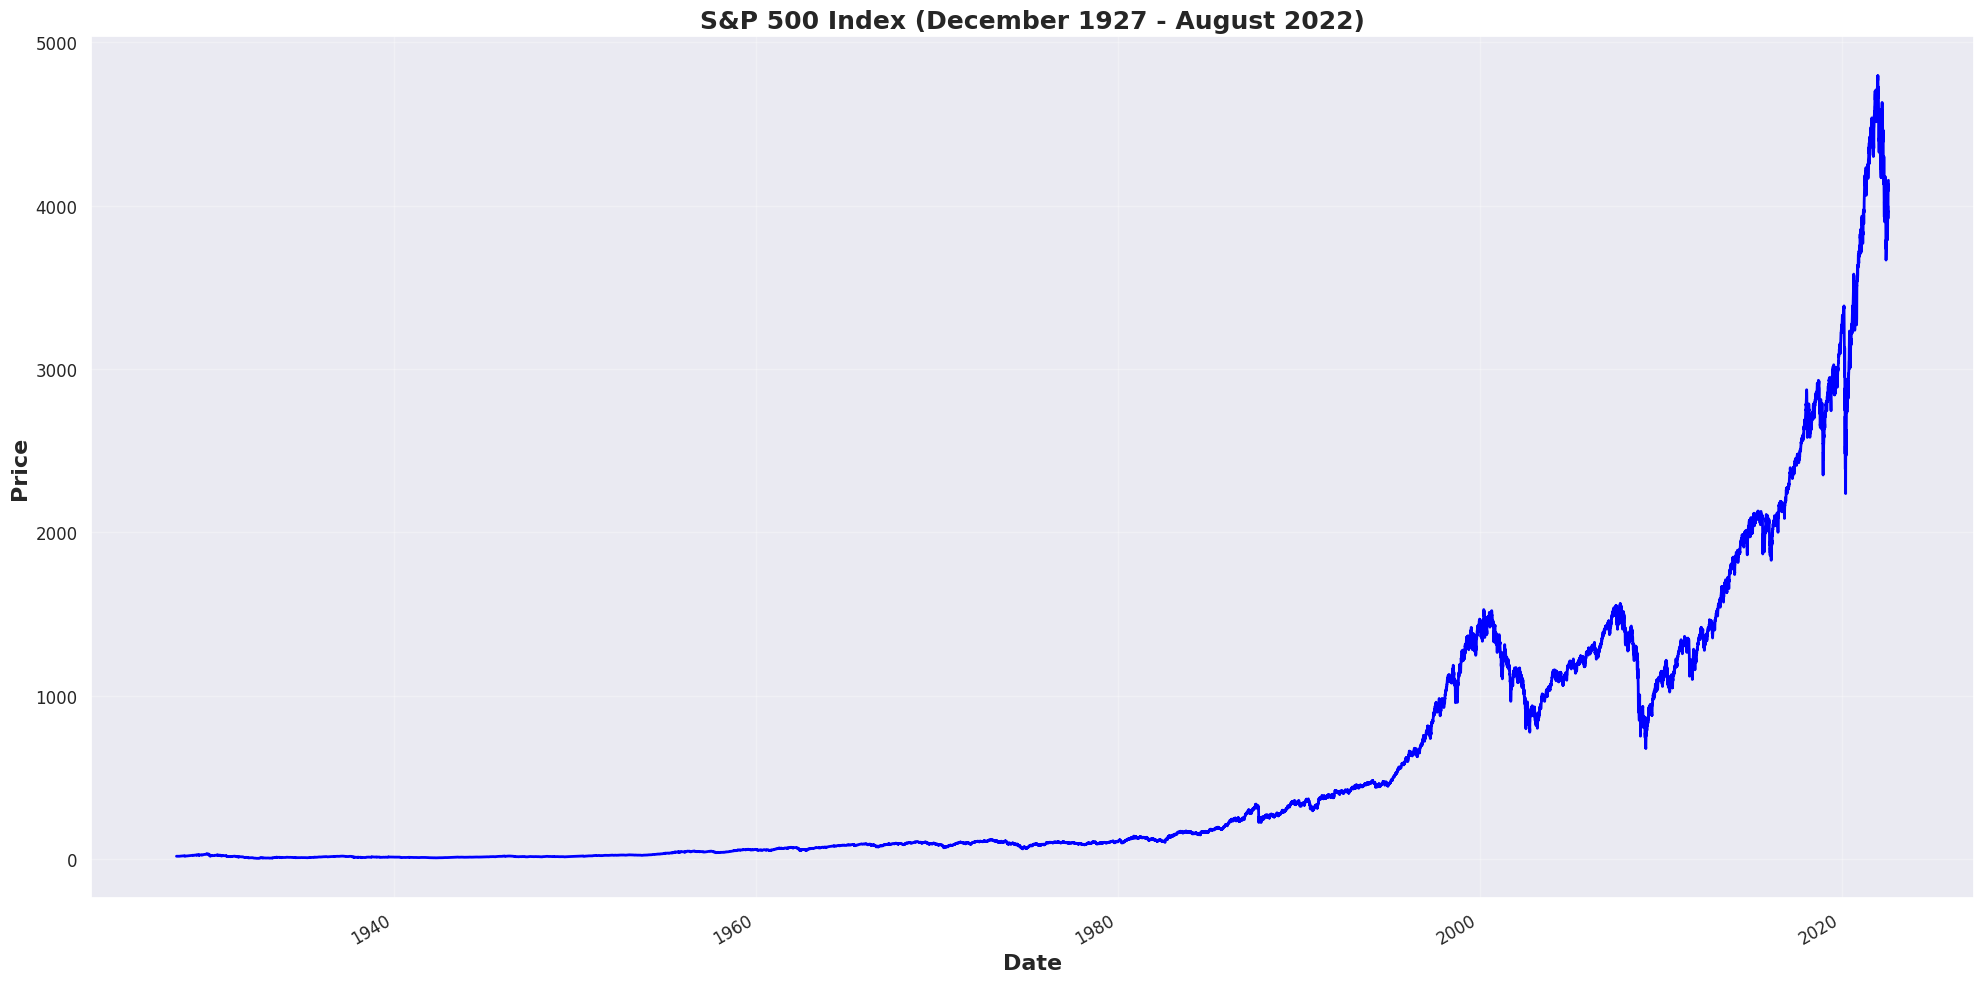
\includegraphics[width=\linewidth]{media/media/image6.png}
\caption{Time series: S\&P 500 Hurst = 0.637, Lag 1, Lag 2 = 300, 400, Time: 30/12/1927 ---- 4/8/2022.}
\label{fig:sp500-hurst-long-ch3}
\end{figure}
\end{landscape}

\begin{landscape}
\begin{figure}[p]
\centering
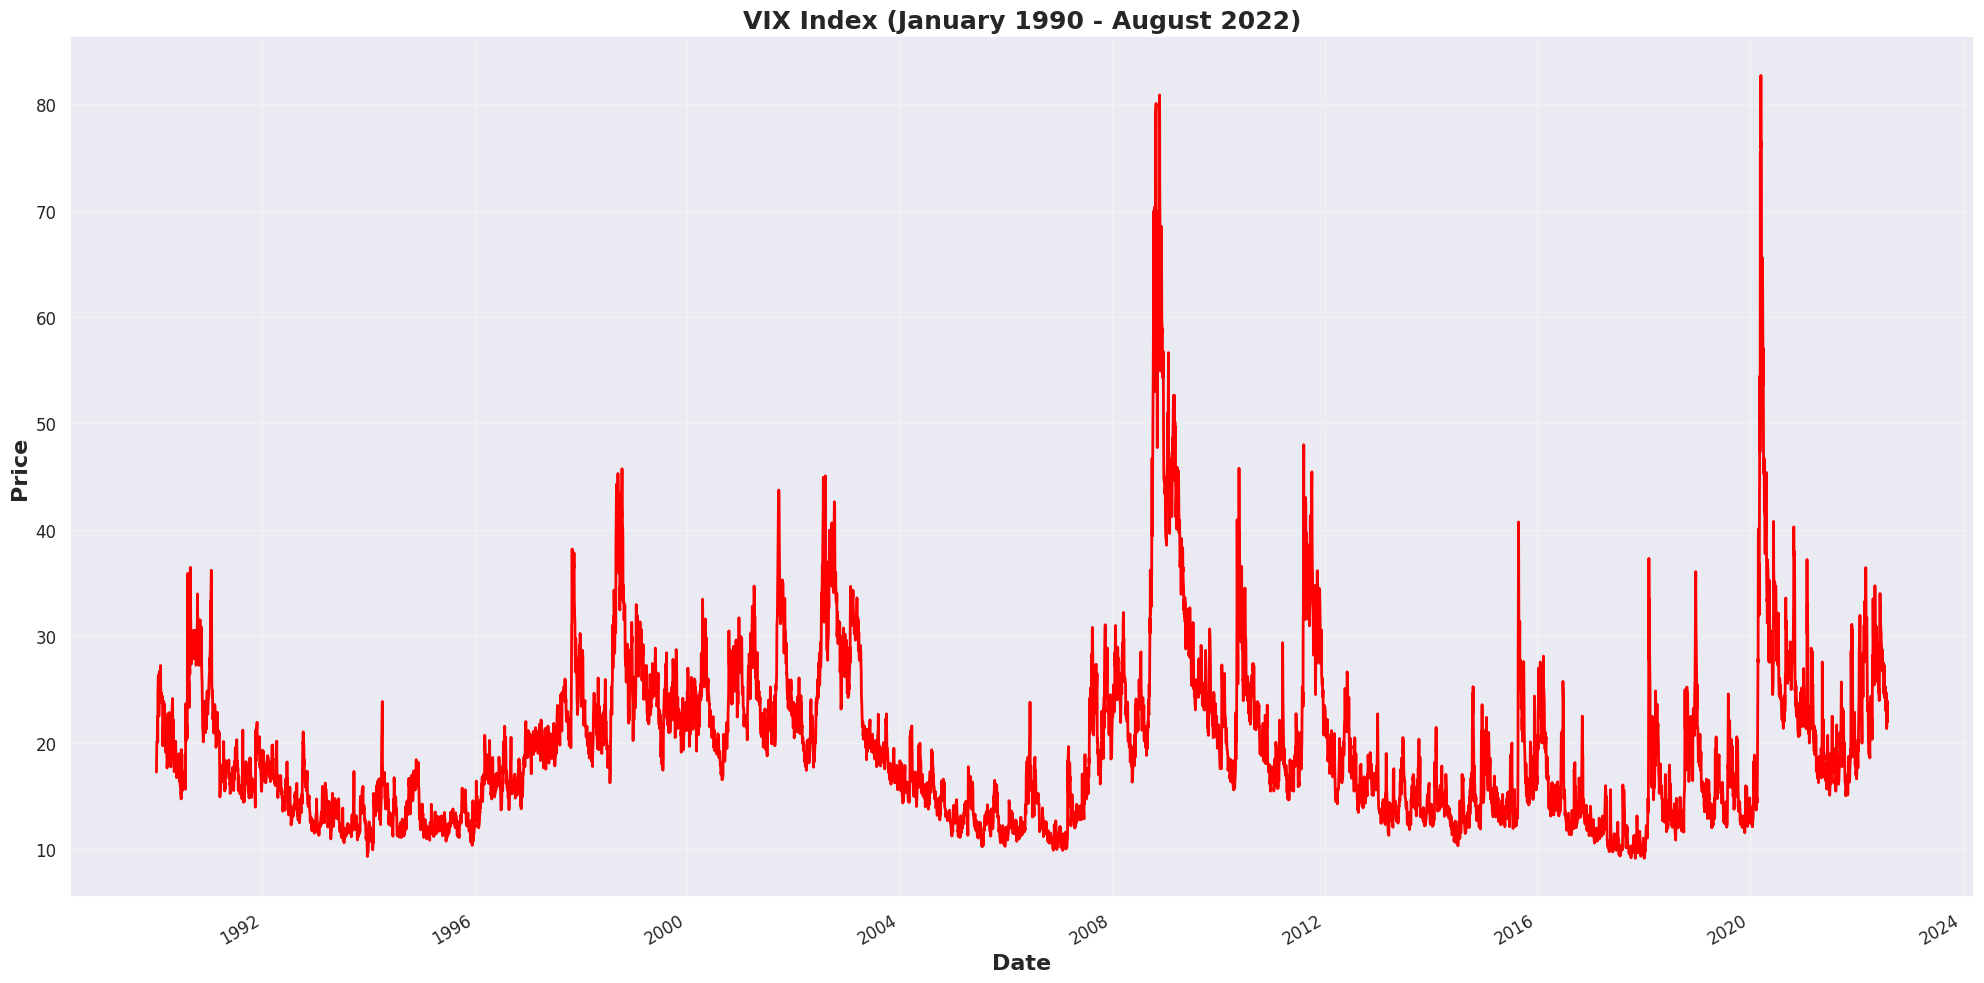
\includegraphics[width=\linewidth]{media/media/image7.png}
\caption{Time Series: VIX Hurst = 0.249, Lag 1, Lag 2 = 300, 400, Time: 02/01/1990 ---- 4/8/2022.}
\label{fig:vix-hurst-ch3}
\end{figure}
\end{landscape}


\begin{landscape}
\begin{figure}[p]
\centering
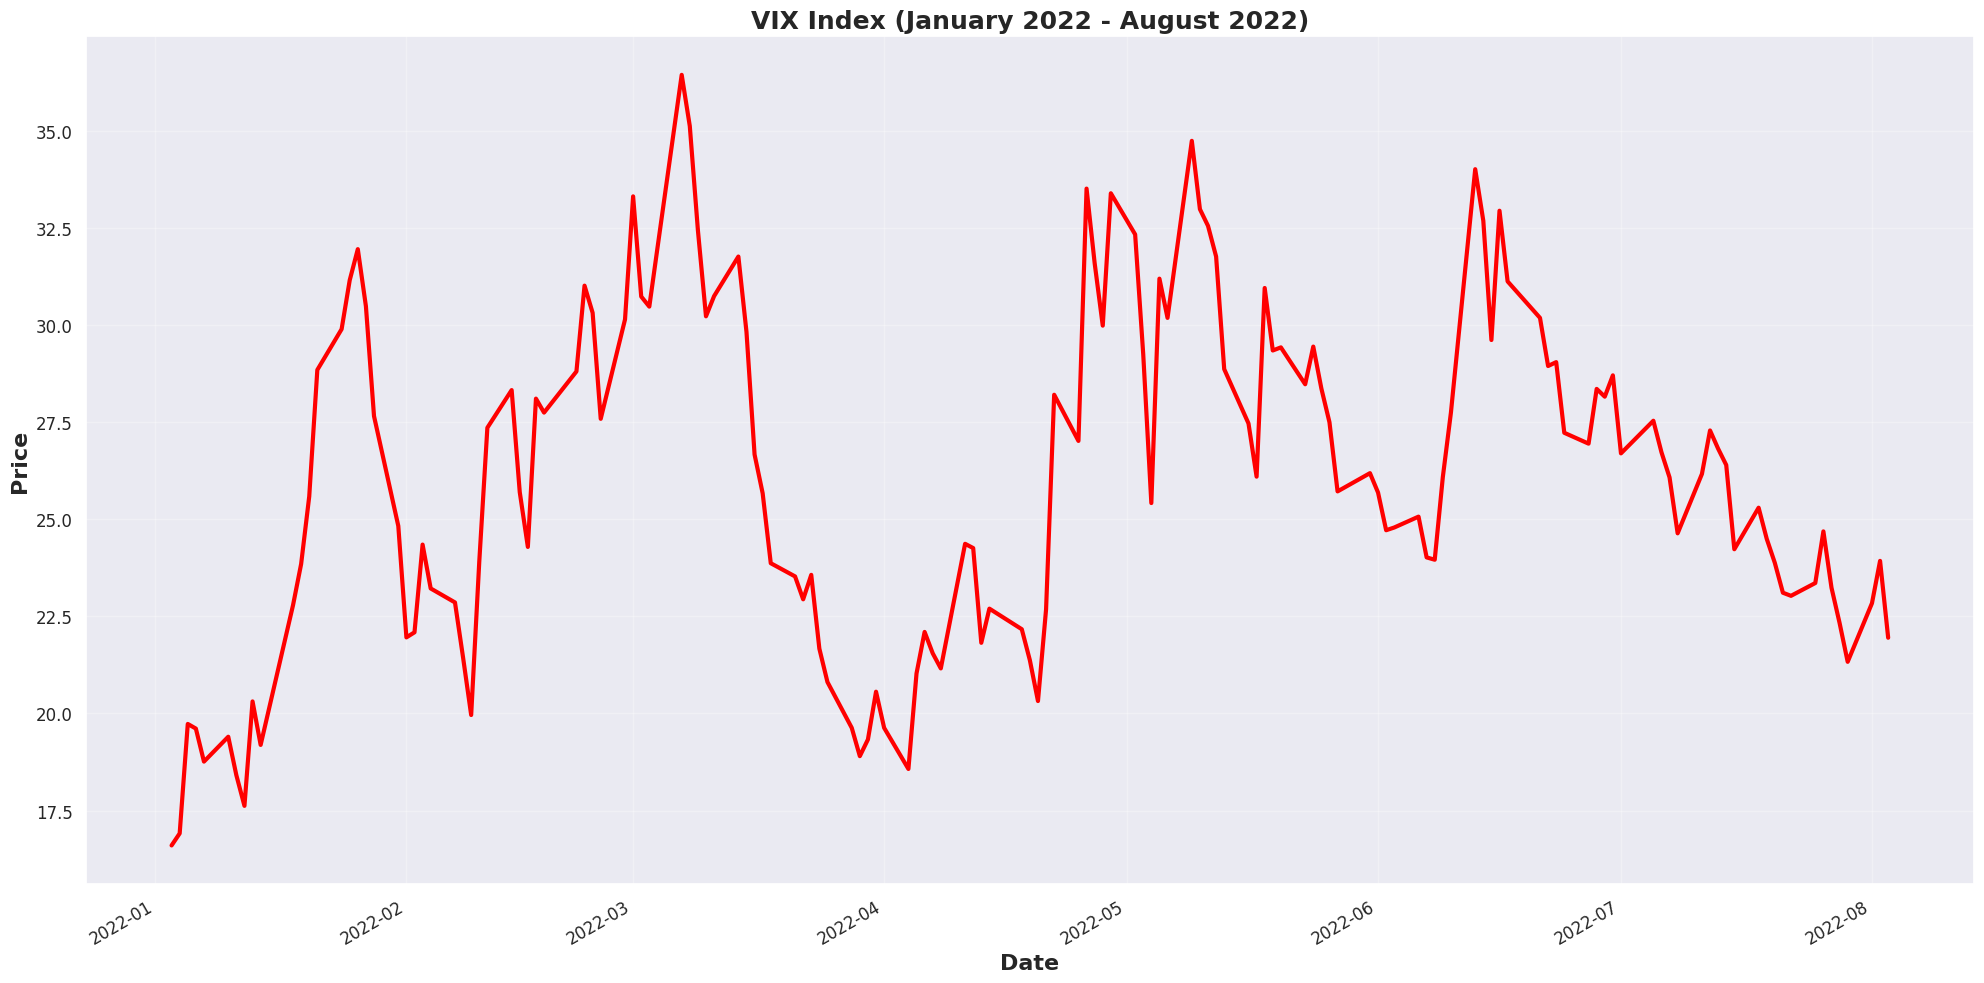
\includegraphics[width=\linewidth]{media/media/image8.png}
\caption{Time Series: VIX Hurst = 0.398, Lag 1, Lag 2 = 2, 20, Time: 03/01/2022 ---- 4/8/2022.}
\label{fig:vix-hurst-short-ch3}
\end{figure}
\end{landscape}

\hypertarget{empirical--analysis--and--model--benchmarking}{%
\section{\texorpdfstring{\emph{\textbf{EMPIRICAL ANALYSIS AND MODEL
BENCHMARKING}}
}{EMPIRICAL ANALYSIS AND MODEL BENCHMARKING }}\label{empirical--analysis--and--model--benchmarking}}

In this section we present the empirical groundwork for the thesis. The
analysis herein, based on our published work, serves two primary
objectives. First, we explore the underlying structure of the VIX time
series using clustering methodologies to identify distinct volatility
regimes. Second, we establish a robust performance benchmark by
implementing and evaluating a suite of forecasting models, from
classical methods to advanced machine learning techniques. The
limitations and characteristics identified in this empirical analysis
provide the essential motivation for the novel theoretical framework
developed in Chapter 5. For full model results and discussions please
see `Notes on Intuitionistic Fuzzy Sets' [P1] and IEEE paper [P4].

\hypertarget{k--means--and--fuzzy--c--means--clustering}{%
\subsection{\texorpdfstring{\emph{K--MEANS AND FUZZY C--MEANS
CLUSTERING}}{K--MEANS AND FUZZY C--MEANS CLUSTERING}}\label{k--means--and--fuzzy--c--means--clustering}}

Determining the optimal number of clusters (K) is crucial for the
effectiveness of the K--Means algorithm. [P1] employed the 'Elbow'
method and 'Silhouette' analysis to find the appropriate value for K.
The Elbow Method plots the sum of squared distances from each point to
its assigned centroid for different values of K. The optimal K is chosen
at the ``elbow`` point, where the rate of decrease sharply slows down.
Silhouette Analysis measures how similar a point is to its own cluster
compared to other clusters, with higher silhouette values indicating
better--defined clusters. In this study, data was normalized using the
StandardScaler technique, which transforms the data to have a mean of 0
and a standard deviation of 1. Normalization is a preprocessing step
used to standardize the range of independent variables or features of
data. This step is essential to ensure that the algorithm treats all
features equally, preventing features with larger ranges from dominating
the clustering process. Figure 3.5 shows as the number of clusters
increase, the error is minimised more and more. Visually, we are looking
for an elbow of this curve. It appears in the region of 2----4 clusters.

\begin{figure}[htbp]
\centering
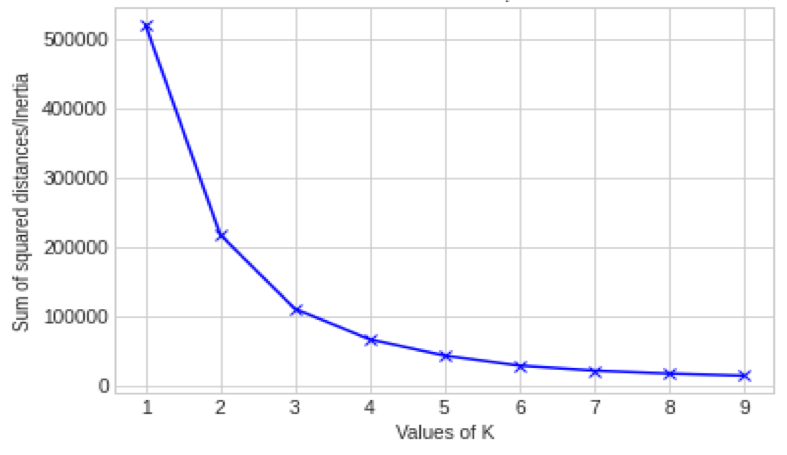
\includegraphics[width=\linewidth,keepaspectratio]{media/media/image19.png}
\caption{Source: [P1] \emph{K--Means Clustering}.}
\label{fig:kmeans}
\end{figure}


The Silhouette method is often compared to the ``Elbow`` method, which
involves plotting the within--cluster sum of squares (WCSS) against the
number of clusters and identifying the point where the rate of decrease
sharply slows. Both methods are used to determine the optimal number of
clusters, but they approach the problem from different angles.

To apply the Silhouette method, we trained K--means clustering for each
value of~k~(the number of clusters). For each clustering configuration,
we computed the silhouette coefficient for every data point and then
averaged these values to obtain the overall silhouette score for that~k.

The Silhouette score for the five--cluster model was found to be 0.554.
This score indicates a reasonably good clustering configuration,
suggesting that the five--cluster model provides a meaningful division of
the data. The Silhouette score, being above 0.5, implies that the
majority of data points are well--matched to their assigned clusters and
only a few points are on the boundary between clusters. While a score
above 0.5 indicates reasonable clustering, the proximity of the score to
0.5 suggests potential overlap between clusters or suboptimal feature
selection. Figure 3.6 shows the silhouette score on y--axis and the
number of clusters on the x--axis. Prior to plotting the clusters, we
find the centroids of the clusters: {[}26.81939959{]},
{[}19.69309811{]}, {[}13.48929072{]}, {[}62.16890411{]},
{[}38.19894207{]}.

\begin{figure}[htbp]
\centering
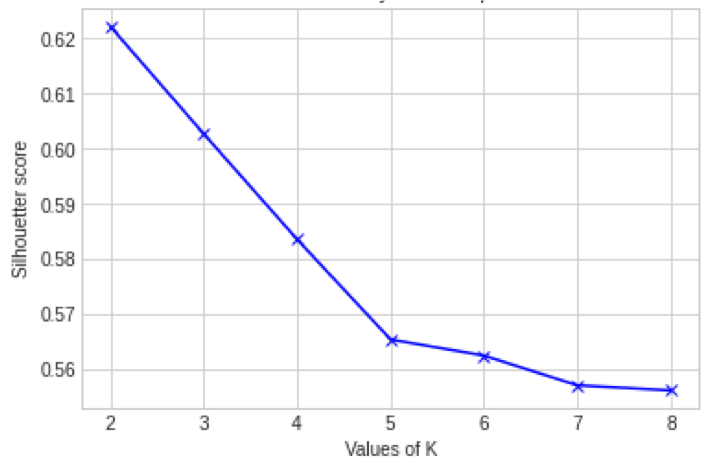
\includegraphics[width=\linewidth,keepaspectratio]{media/media/image20.png}
\caption{Source: [P1] \emph{Silhouette method}.}
\label{fig:silhouette-method}
\end{figure}


Next, we plot the graph with 2 and 5 clusters. The top graph in Figure
3.7 shows two clusters identified by horizontal lines and the bottom
graph with 5 clusters identified also by the horizontal lines. The top
graph simply splits the data into periods of low and high volatility.
The graph shows when the volatility is low it tends to stay low and when
it is high it tends to remain high. The bottom graph has 5 centroids
which are represented as horizontal lines. The graph splits the data
into periods of very low volatility, low volatility, medium volatility,
high volatility, and extremely high volatility.

To understand the dynamics of volatility transitions, we calculated the
transition matrix for the clusters. The transition matrix showed how
many times the Volatility Index (VIX) moved from one cluster to another
over the observed period. This matrix is crucial for capturing the
temporal behaviour of volatility and understanding the stability and
transitions between different volatility states.

The expectation was that the transition matrix would be symmetric if
there were no significant jumps in VIX. However, the matrix was not
symmetric, indicating the presence of jumps and non--uniform transitions
between volatility states. This asymmetry suggests that certain states
of volatility are more likely to transition into others, rather than
remaining stable or reverting, highlighting the dynamic nature of
financial markets.

\begin{figure}[htbp]
\centering
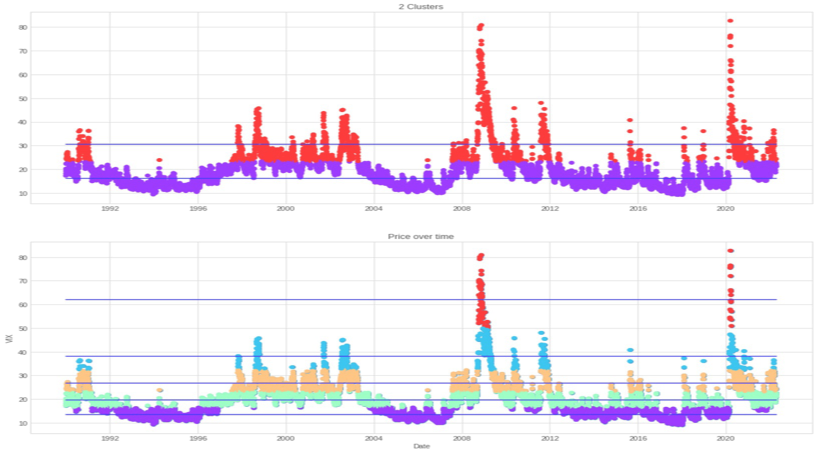
\includegraphics[width=\linewidth,keepaspectratio]{media/media/image21.png}
\caption{K-means clustering of VIX levels comparing different cluster configurations (1990--2022). Top panel: Binary classification into low volatility (purple) and high volatility (red) regimes. Bottom panel: Five-cluster solution distinguishing very low, low, medium, high, and extreme volatility states. Horizontal lines indicate cluster boundaries. Asymmetric transitions between clusters reveal the presence of volatility jumps. Source: [P1].}
\label{fig:results}
\end{figure}

Fuzzy C--Means (FCM) clustering is an advanced clustering algorithm that
extends the traditional K--means clustering by allowing data points to
belong to multiple clusters with varying degrees of membership. This
approach is particularly advantageous in scenarios where the boundaries
between clusters are not well--defined, enabling a more flexible and
nuanced understanding of the data structure. In hard clustering, data
are divided into distinct clusters, where each data point can only
belong to one cluster. In fuzzy clustering, data points can belong to
multiple clusters. Fuzzy C--means clustering's ability to assign
fractional membership is particularly valuable in financial volatility
analysis, where transitions between states (e.g., medium to high
volatility) may exhibit gradual shifts rather than discrete jumps. For
example, an apple can be red or green (hard clustering), but an apple
can also be red and green (fuzzy clustering). Here, the apple can be red
to a certain degree as well as green to a certain degree. Instead of the
apple belonging to green {[}green = 1{]} and not red {[}red = 0{]}, the
apple can belong to green {[}green = 0.5{]} and red {[}red = 0.5{]}.
These values are normalized between 0 and 1; however, they do not
represent probabilities, so the two values do not need to add up to 1.
Membership grades are assigned to each of the data points. These
membership grades indicate a degree to which data points belong to each
cluster. Thus, points on the edge of a cluster, with lower membership
grades, may be~in the cluster~to a lesser degree than points in the
centre of cluster. Figure 3.8 illustrates Fuzzy C--Means Clusters 0 ---
4.

\begin{figure}[htbp]
\centering
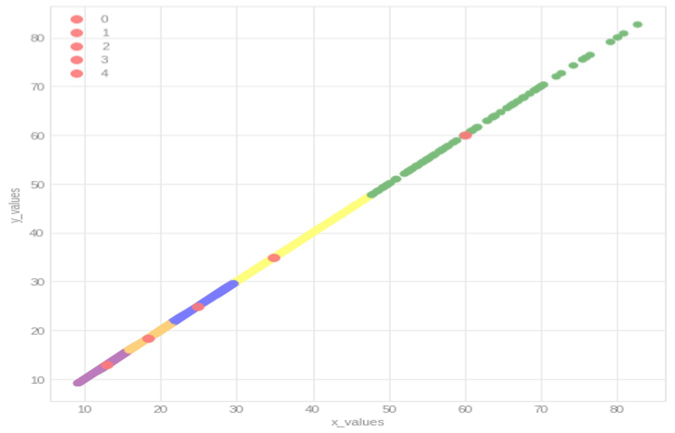
\includegraphics[width=6.5in,height=4.16944in,keepaspectratio]{media/media/image22.png}
\caption{Fuzzy C-Means (FCM) cluster centroids for VIX volatility regimes. The five clusters (0--4) represent increasing volatility levels from very low (~10--15) to extreme (~80). Unlike hard clustering, FCM assigns fractional membership degrees, allowing data points near cluster boundaries to belong partially to multiple regimes. Source: [P1].}
\label{fig:results-3-22}
\end{figure}


In figure 3.9 we plot the best Cluster 5 with 5 centroids, which are
represented as horizontal lines. The graph splits the data into periods
of very low volatility, low volatility, medium volatility, high
volatility, and extremely high volatility according to FCM algorithm.

The Silhouette Score is 0.555 which in this case is not very different
to K--Means and is probably due to random state initialisation. It
suggests that the clusters are somewhat well--separated but may not be
perfectly distinct. While it's not as high as it could be, it still
indicates a reasonable level of cluster quality. The proximity of the
score to 0.5 suggests that there might be some overlap or inconsistency
in the clusters.

\begin{figure}[htbp]
\centering
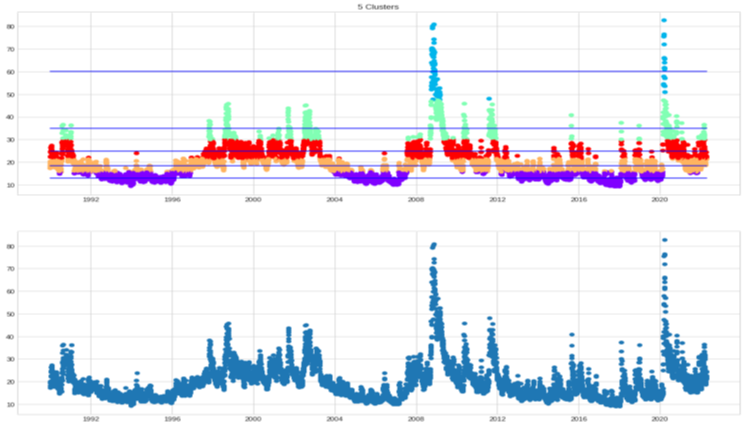
\includegraphics[width=\linewidth,keepaspectratio]{media/media/image23.png}
\caption{K-means clustering of VIX levels into five volatility regimes (1990--2022). Top panel: VIX values color-coded by cluster assignment, with horizontal lines indicating cluster boundaries. Bottom panel: Raw VIX time series for reference. Notable spikes correspond to the 2008 financial crisis and COVID-19 pandemic. Source: [P1].}
\label{fig:results-3-23}
\end{figure}

\FloatBarrier

\hypertarget{deep--neural--network--models}{%
\subsection{\texorpdfstring{\emph{DEEP NEURAL NETWORK MODELS}
}{DEEP NEURAL NETWORK MODELS }}\label{deep--neural--network--models}}

While clustering methods provide valuable insights into volatility
regimes, deep neural networks offer complementary tools for time--series
forecasting by capturing temporal dependencies and nonlinear patterns.
To establish a performance baseline, a range of forecasting models were
implemented and tested on the daily VIX log--return series.

\hypertarget{methodology--dnn}{%
\subsubsection{Methodology}\label{methodology--dnn}}

In the previous sections we already presented the theoretical framework of
the models discussed here. A walk--forward validation approach was used.
The models ranged from a Naïve forecast and ARIMA to more complex
architectures like LSTM, NBEATS, and a hybrid GAN--SVM/RF framework. In
the hybrid approach, an ARIMA model was first used to capture linear
trends. A Generative Adversarial Network (GAN) was then trained, with an
LSTM--based Generator and a CNN--based Discriminator, to learn the
non--linear data distribution and generate synthetic time--series
features. These generated features were then used as inputs for Support
Vector Machine (SVM) and Random Forest (RF) models to make the final
forecast. The 93.3\% accuracy metric refers specifically to the internal
training accuracy of the GAN's discriminator in distinguishing real from
generated data. It is not a forecasting performance metric.

In this section we outline results from [P4]. As was already
mentioned, we ran our data from January 1990 to April 2022 for a total
of 1200 epochs and it gave us the accuracy rate of 93.3\%.

\begin{figure}[htbp]
\centering
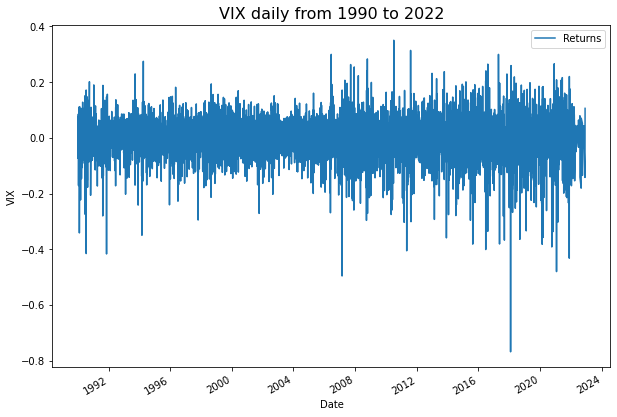
\includegraphics[width=\linewidth,keepaspectratio]{media/media/image24.png}
\caption{Daily log returns of the VIX index (1990--2022). The series exhibits volatility clustering, with periods of high volatility (e.g., 2008, 2020) followed by gradual mean reversion. The stationary nature of log returns is confirmed by ADF testing. Source: [P4].}
\label{fig:3-24}
\end{figure}


In this paper, we used normalised log scale return VIX (Figure 3.10) as our train data
and normalised log scale return VVIX as our validation data. While
standard validation practice involves using a hold--out set of the same
time series, a different approach was intentionally employed here to
test a deeper aspect of the research hypothesis. The central premise of
this thesis is that VVIX, as the ``volatility of volatility'', is not
merely a separate index but is intrinsically linked to the process that
generates VIX dynamics. VVIX can be considered a market--based proxy for
the latent stochastic volatility process driving the VIX (Figure 3.11).

Therefore, using VVIX as the validation set was not intended to measure
direct forecasting accuracy in the traditional sense. Instead, it was
designed as a stringent test of model generalisation and robustness. The
objective was to determine if a model trained exclusively on VIX data
could learn the underlying structural dynamics of volatility deeply
enough to generate outputs that correlate with, or statistically similar
to, the behaviour of its own driving process (VVIX).

A successful validation in this context means the model's outputs on the
validation set share statistical properties with the actual VVIX data
and would provide strong evidence that the model has captured more than
just superficial autocorrelation in the VIX series. It would suggest
that the model has learned a fundamental aspect of the volatility
generation process itself, thereby strengthening the case for using
VVIX--related dynamics in future, more advanced forecasting models. See
the graph below please.

\begin{figure}[htbp]
\centering
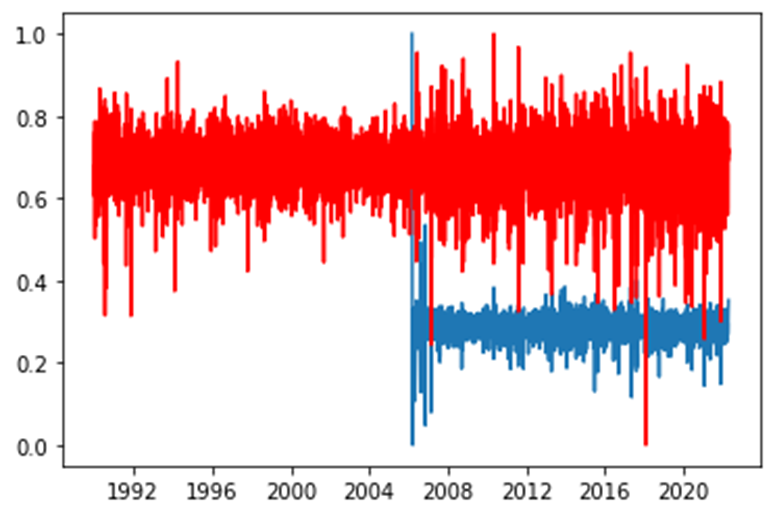
\includegraphics[width=4.37296in,height=2.91139in,keepaspectratio]{media/media/image25.png}
\caption{Comparison of normalised log returns: VIX (red) and VVIX (blue) from 1990--2022. VVIX data begins in 2006. Both series are scaled to [0,1] range to facilitate comparison. The co-movement suggests VVIX (volatility of volatility) captures similar market dynamics as VIX. Source: [P4].}
\label{fig:3-25}
\end{figure}


We built ARIMA on scaled data and predict the fitted values on
validation data. We also calculated the future trend growth with ARIMA.
We then made a data frame of the fitted values and split it into train
and test sets for our GAN model. ARIMA was used to capture long--term
trends and reduce noise in the data, providing a stable baseline for our
GAN--based feature generation. The combination leverages ARIMA's
strengths in linear modelling and GANs' ability to model complex,
nonlinear relationships. We added CNN conv1 layer as our discriminator
and choose accuracy as our metric. Then in generator we used two layers
of CNN and LSTM together and again we chose accuracy as our metrics. For
training the model, we compiled discriminator and generator together and
used the learning rate of 0.001 and beta of 0.5. We ran the model for a
total of 1200 epochs and it gave us the internal training accuracy of
the GAN's discriminator of 93.3\%. We then used the fitted (predicted)
values of GAN as features/inputs in SVM and RF. We defined the RF model
and used train features for training and fitting and test features for
predicting. The results for MAPE and MAE are quite encouraging. For SVM,
we used grid search and fit the model to get a score of 98.5\% on
fitting.

Methodology

This study proposes a hybrid forecasting framework that combines a
classical time series model (ARIMA), a deep generative model (GAN), and
traditional machine learning regressors (SVM, RF) to predict financial
volatility. The workflow consists of three main stages.

Stage 1: Data Pre--processing and Trend Extraction with ARIMA

First, the historical time series data was scaled to the range {[}--1,
1{]}. An ARIMA model was then fitted to this scaled data. The primary
purpose of the ARIMA model was to capture the long--term linear trends
and autoregressive patterns (i.e., the ``memory``) in the series. The
fitted values from the ARIMA model serve as a smoothed, detrended
baseline, which is then used as the input for the subsequent generative
model. This approach leverages ARIMA's strength in linear modelling to
provide a more stable foundation for the GAN.

Stage 2: Synthetic Feature Generation with a GAN

A Generative Adversarial Network (GAN) was developed to learn the
complex, non--linear dynamics of the ARIMA--fitted time series and
generate synthetic data with the same statistical properties. The
generated data is then used as an input feature for the final prediction
models.

\begin{itemize}
\item
  Generator Architecture: The generator is an LSTM--based recurrent
  neural network. It takes a random noise vector from a latent space of
  size 100 as input. This input is processed through two sequential LSTM
  layers, which are designed to learn and generate temporal patterns.
  The final layer is a Dense layer that outputs a sequence of the
  desired length, matching the input time series.
\item
  Discriminator Architecture: The discriminator is a Convolutional
  Neural Network (CNN) designed for 1D sequence classification. It
  consists of a Conv1D layer followed by LeakyReLU activation and Dense
  layers. Its task is to distinguish between the real ARIMA--fitted
  sequences and the synthetic sequences produced by the generator.
\item
  Training: The GAN was trained for 1200 epochs. The generator and
  discriminator were compiled together using an Adam optimizer with a
  learning rate of 0.001 and a beta\_1 of 0.5. The training objective
  was to achieve high accuracy in the discriminator, indicating that the
  generator was producing high--quality, realistic time series data. The
  final internal training accuracy of the discriminator reached 93.3\%.
\end{itemize}

Stage 3: Final Prediction with SVM and Random Forest

The trained GAN generator was used to produce a sequence of predicted
values. These generated values, which encapsulate the non--linear
patterns learned by the GAN, were used as input features for two final
regression models: a Support Vector Machine (SVM) and a Random Forest
(RF).

\begin{itemize}
\item
  Random Forest (RF): The RF model was trained on a training set of the
  GAN--generated features and evaluated on a test set.
\item
  Support Vector Machine (SVM): A grid search was performed to optimize
  the hyperparameters for the SVM model, which was then trained and
  fitted on the same data, achieving a high fitting score.
\end{itemize}

The performance of both models was evaluated using Mean Absolute
Percentage Error Mean Absolute Error (MAE).

Comprehensive Architectural Summary

1. Data Representation and Preprocessing

Each 100-point time-series segment is first reshaped into a 10$\times$10 grid,
padded to 32$\times$32 (added zeros around it to become 32x32), and treated as
a single-channel ``image'' so that convolutional layers can process it.
Both training and test sets are cast into~(N, 32, 32, 1)~tensors before
model training.

2. Generative Adversarial Network (GAN)

Discriminator

\begin{itemize}
\item
  Input:~(32, 32, 1)~images. (height, width, number of channels ---- 1
  greyscale, 3 for RGB).
\item
  Architecture: Four Conv2D blocks with 128 filters, 3$\times$3 kernels, stride
  2, each followed by LeakyReLU ($\alpha$\,=\,0.2) and Dropout (0.25);
  flattened to a Dense(1, sigmoid) output.
\item
  Optimizer: Adam (lr\,=\,2$\times$10\textsuperscript{--4}, $\beta$\textsubscript{1}\,=\,0.5).
\item
  Loss: Binary cross-entropy
\end{itemize}

Generator (Conv2DTransposed variant)

\begin{itemize}
\item
  Input: latent vector~z~of dimension 100.
\item
  Architecture: Dense(128$\cdot$4$\cdot$4) $\rightarrow$ LeakyReLU $\rightarrow$ Reshape(4,4,128); three
  Conv2DTranspose(128, 4$\times$4, stride\,2, padding\,``same'') blocks each
  with LeakyReLU; final Conv2D(1, 3$\times$3, tanh) producing
  a~(32,32,1)~sample.
\item
  Optimizer: Adam (lr\,=\,2$\times$10\textsuperscript{--4}, $\beta$\textsubscript{1}\,=\,0.5).
\item
  Loss: Binary cross-entropy
\end{itemize}

Alternative Generator (1-D Conv + LSTM)

An additional prototype replaces Conv2DTranspose with a Time Distributed
Conv1D stack, followed by two Bidirectional LSTM(100) layers and dense
blocks; output is again reshaped to~(32,32,1)

GAN Assembly and Training

\begin{itemize}
\item
  The GAN freezes the discriminator during generator updates and trains
  with Adam (lr\,=\,10\textsuperscript{--4}, $\beta$\textsubscript{1}\,=\,0.5)
\item
  Real sample generation: random index sampling from the training set
  with label~1
\item
  Fake sample generation: generator output with label~0
\item
  Training loop: for each step, update discriminator on real and fake
  batches, then update generator via GAN loss; invoked
  with~latent\_dim=100, 20 epochs, batch size 64
\end{itemize}

3. Downstream Forecasting (Conceptual)

The GAN's synthetic samples are intended as features for a hybrid
CNN----LSTM forecaster. The alternative generator
(Conv1D\,+\,Bidirectional LSTM) illustrates how convolutional layers
extract local patterns, while LSTMs model temporal dependencies before
projecting back to the 32$\times$32 grid.

\begin{longtable}[]{@{}
  >{\raggedright\arraybackslash}p{(\columnwidth - 2\tabcolsep) * \real{0.4180}}
  >{\raggedright\arraybackslash}p{(\columnwidth - 2\tabcolsep) * \real{0.5820}}@{}}
\toprule
\begin{minipage}[b]{\linewidth}\raggedright
Component
\end{minipage} & \begin{minipage}[b]{\linewidth}\raggedright
Key Settings
\end{minipage} \\
\midrule
\endhead
Latent dimension & 100 \\
Batch size & 64 \\
Epochs & 20 \\
Discriminator optimizer & Adam (2$\times$10\textsuperscript{--4}, $\beta$\textsubscript{1}=0.5) \\
Generator optimizer & Adam (2$\times$10\textsuperscript{--4}, $\beta$\textsubscript{1}=0.5) \\
GAN optimizer & Adam (1$\times$10\textsuperscript{--4}, $\beta$\textsubscript{1}=0.5) \\
Dropout & 0.25 in discriminator blocks \\
Activation & LeakyReLU ($\alpha$=0.2); tanh output \\
\bottomrule
\end{longtable}

\begin{itemize}
\item
  Data Representation (10x10 grid, 32x32 image): A pre--processing trick.
  The 1D time series (100 points long) is reshaped into a 2D 10x10 grid,
  which is then ``padded`` (zeros added around it) to become a 32x32 grid.
  This is done so that 2D CNNs, which are powerful pattern detectors,
  can be used.
\item
  Tensor: The primary data structure used in deep learning. It's a
  multi--dimensional array. A tensor with shape (N, 32, 32, 1)
  represents:

  \begin{itemize}
  \item
    N: Batch size (number of samples).
  \item
    32: Height of the ``image.``
  \item
    32: Width of the ``image.``
  \item
    1: Number of channels (1 for grayscale, 3 for a color RGB image).
  \end{itemize}
\item
  Conv2D: A 2D Convolutional Layer. It slides a small window (kernel)
  over a 2D input (like the 32x32 image) to detect spatial patterns.
\item
  Filters (e.g., 128 filters): The number of different pattern--detectors
  in a convolutional layer. More filters allow it to learn more complex
  patterns.
\item
  Kernel (e.g., 3x3): The size of the ``window`` that scans the input. A
  3x3 kernel looks at a 3x3 pixel area at a time.
\item
  Stride (e.g., stride 2): The number of pixels the kernel jumps as it
  scans the input. A stride of 2 (instead of 1) moves 2 pixels at a
  time, which effectively downsamples the image (makes it smaller).
\item
  Dropout (e.g., 0.25): A regularization technique to prevent
  overfitting (where the model just memorizes the training data). During
  training, it randomly ``drops`` (sets to zero) a fraction (e.g., 25\%)
  of neurons, forcing the network to learn more robust patterns.
\item
  Flattened: A layer that converts a multi--dimensional tensor (like the
  output of a CNN) into a single 1D vector, typically to feed it into a
  Dense layer.
\item
  Conv2DTranspose (or Deconvolution): The ``opposite`` of a Conv2D layer.
  It's used to upscale a small input into a larger output. The generator
  uses this to go from its small latent vector (reshaped to 4x4x128) up
  to the final 32x32x1 ``image.``
\item
  Padding (``same``): A setting for a convolutional layer. It adds pixels
  (usually zeros) around the border of the input so that the output
  feature map has the same height and width as the input (when
  stride=1).
\item
  Conv1D: A 1D Convolutional Layer. Similar to Conv2D, but it scans a 1D
  sequence. It's excellent for finding local patterns in time series or
  text.
\item
  TimeDistributed: A special wrapper layer. It applies another layer
  (like a Conv1D) to every individual time--step of an input sequence.
  This allows a CNN to process each part of a sequence before it's fed
  to an RNN (like an LSTM).
\item
  Batch Size (e.g., 64): The number of data samples processed in one
  iteration of training before the model's weights are updated.
\end{itemize}

We decompose volatility dynamics into linear and nonlinear components.
An ARIMA model, fitted in a rolling, leakage--free manner to normalised
VIX log--returns, provides a denoised baseline and/or residuals. On top,
we train a GAN with an LSTM--based generator and a lightweight Conv1D
discriminator to produce time--series features that are statistically
indistinguishable from ARIMA--processed sequences. The downstream
forecasters (SVM and Random Forest) consume these generated features to
predict the next--step return. Training uses Adam with $\beta$1=0.5 and a small
learning rate; in practice we prefer TTUR
(lrD\_DD\hspace{0pt}\textgreater lrG\_GG\hspace{0pt}) and WGAN--GP for
stability, together with early stopping monitored by distributional and
temporal similarity metrics (e.g., MMD, ACF/PSD alignment) rather than
discriminator accuracy. We evaluate forecast skill on VIX via MAE, RMSE,
and sMAPE/MASE with Diebold----Mariano tests against Naïve, ARIMA,
residual LSTM, and N--BEATS baselines. Separately, we validate
representation robustness on VVIX (volatility--of--volatility) as a
domain--shift test, reporting correlation, spectral and Hurst/DFA
similarity, and TSTR performance, to evidence that the learned
representation captures structural drivers beyond mere autocorrelation.

\begin{figure}[p]
\centering
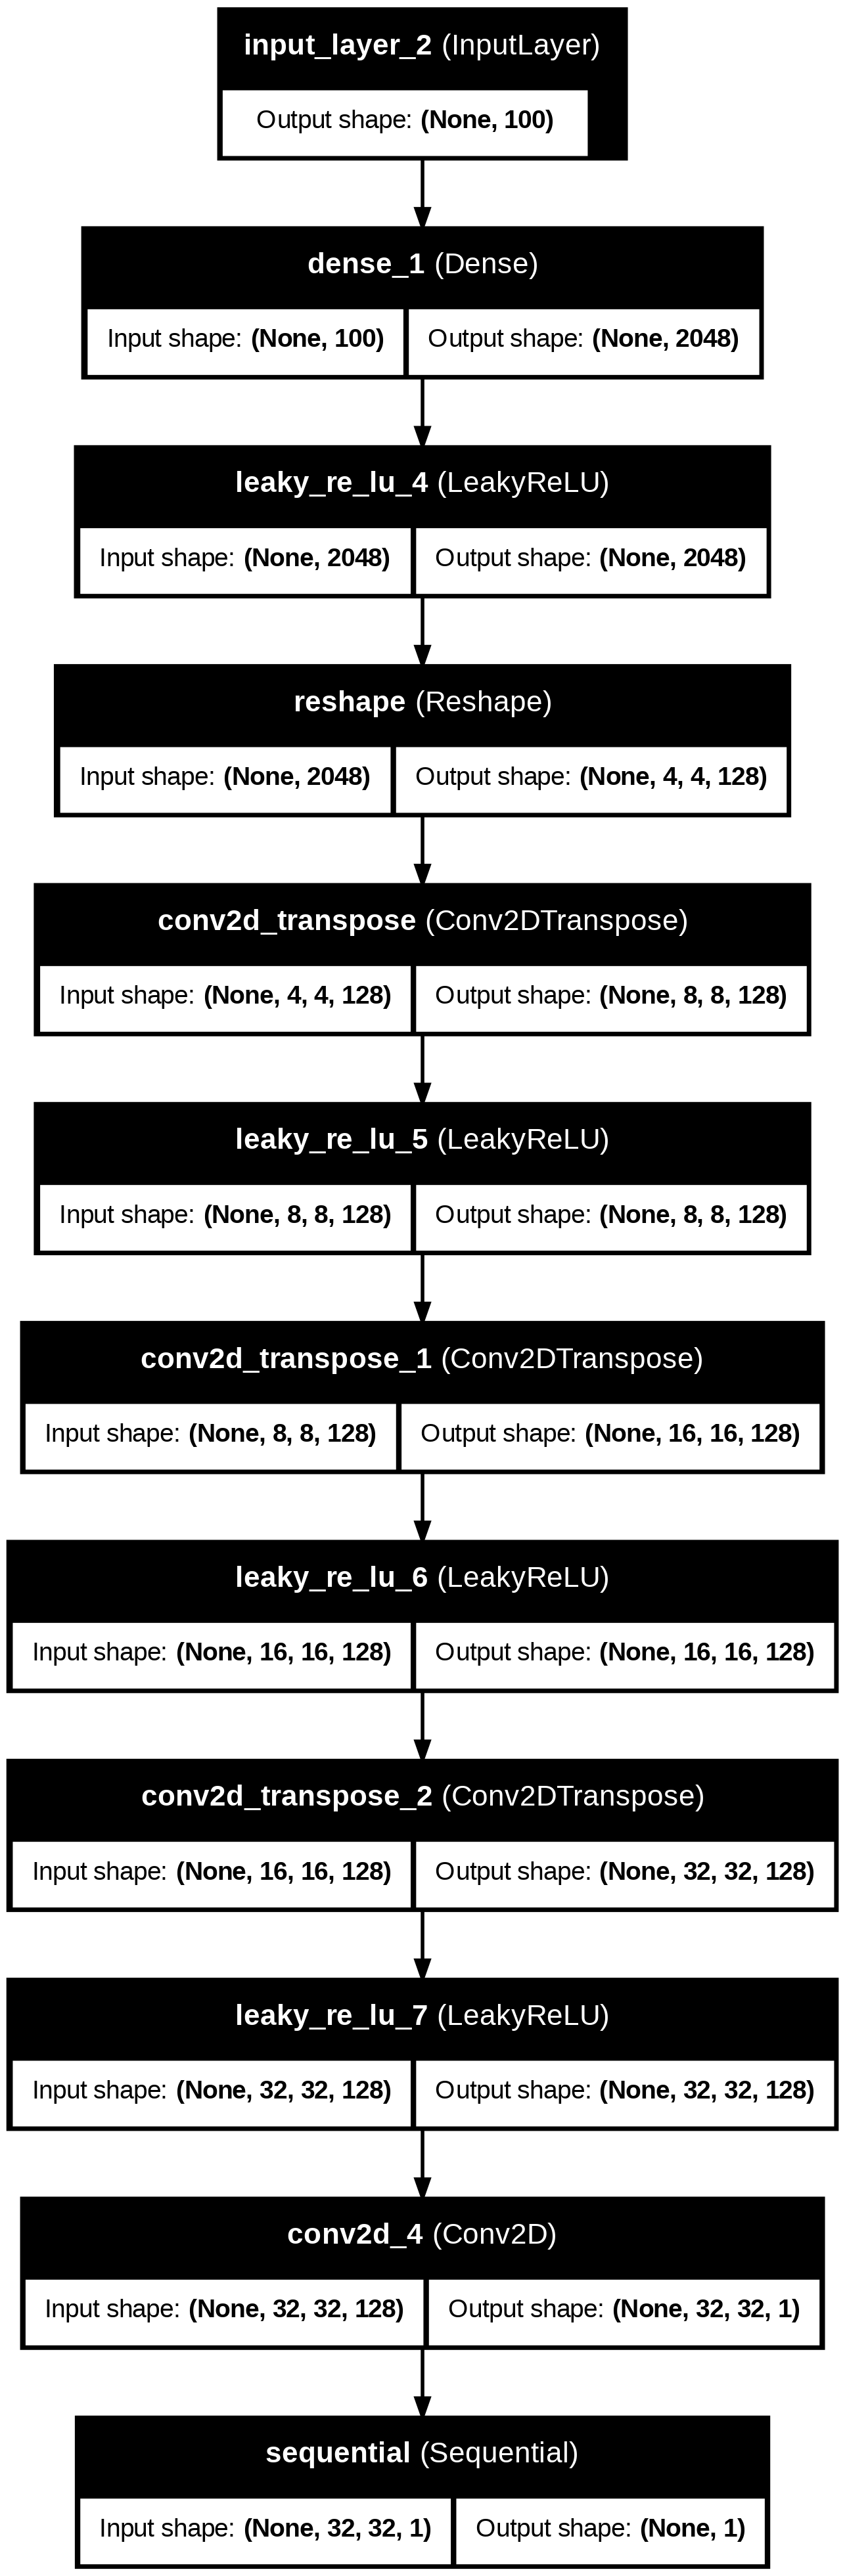
\includegraphics[width=3.10417in,height=9in,keepaspectratio]{media/media/image27.png}
\caption{Source: [P4] DNN Architecture.}
\label{fig:3-26}
\end{figure}

Figure 3.12 represents the architecture of a deep neural network with
several dense (fully connected) layers and Leaky ReLU activation
functions that we used in our modelling. This deep neural network
architecture is composed of multiple layers that work together to
process and predict data effectively. It begins with an input layer,
labelled input\_1, which accepts input data of shape (None, 100). Here,
``None`` indicates that the network can handle batches of any size, while
each sample in the batch has a feature vector of size 100. This input
layer serves as the foundation for subsequent transformations and
computations throughout the network.

The architecture incorporates several fully connected (dense) layers
that progressively refine and process the input data. The first dense
layer maps the 100--dimensional input to a 256--dimensional space,
outputting (None, 256). A second dense layer retains this
dimensionality, allowing deeper feature representation. Following these,
the third dense layer expands the feature space to 512 dimensions, and
the fourth layer continues processing within this 512--dimensional space.
The final dense layer aggregates all the features to produce a single
scalar output per input sample, which we use for predicting continuous
values.

To enhance the learning capabilities of the network, each dense layer is
followed by a Leaky ReLU activation function. Unlike the standard ReLU,
which can cause ``dying neurons`` due to zero gradients for negative
inputs, Leaky ReLU allows a small gradient for negative values, ensuring
better gradient flow throughout the network and maintaining learning
efficiency.

A reshape layer is included near the output, modifying the dense layer's
output into a specific shape of (None, 32, 32, 1). We used this to
structure the data for further processing for convolutional operations.
The final output layer is sequential and produces a single scalar value
per input sample.

This architecture is highly flexible and versatile. The fully connected
layers enabled it to handle a variety of input data types, while the use
of Leaky ReLU ensured stable training and prevents the vanishing
gradient problem. Its depth allows it to capture complex hierarchical
features, and the reshape layer adds adaptability for downstream tasks

\hypertarget{results}{%
\subsubsection{Results}\label{results}}

RF MAPE: 0.007 and MAE: 0.005. SVM MAPE: 0.006 and MAE: 0.004.

The MAPE and MAE values of 0.006 and 0.004 for SVM indicate excellent
predictive accuracy, outperforming baseline models like ARIMA and even
certain deep learning approaches. While NBEATS slightly outperforms
Conv1D and LSTM in terms of MAE and MSE, its architecture may be less
effective for high--frequency financial data where local patterns
dominate, highlighting the need for task--specific tuning.

% Figure 3.13
\begin{figure}[p]
\centering
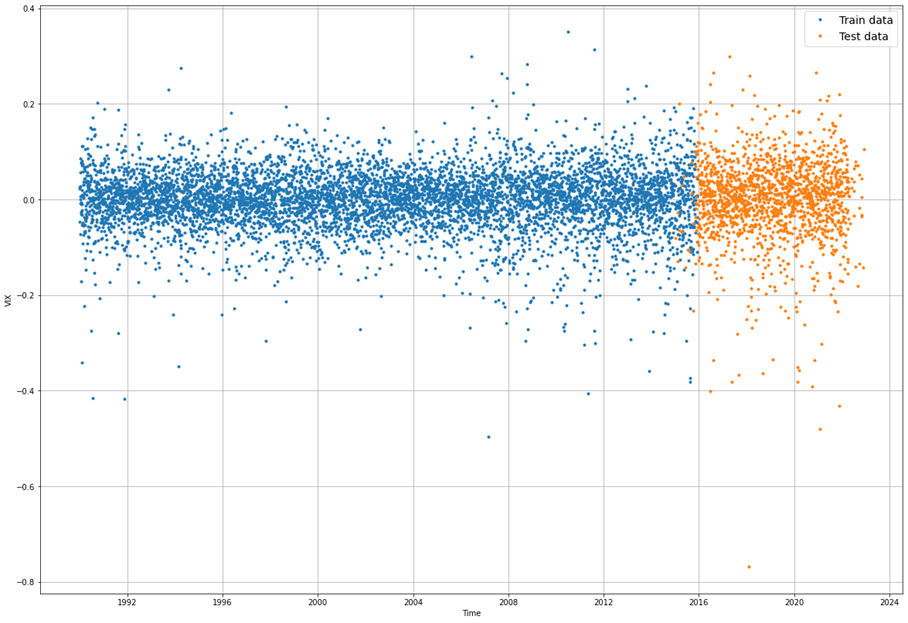
\includegraphics[width=\linewidth,keepaspectratio]{media/media/image28.png}
\caption{Train and test split (source: [P4]).}
\label{fig:train-test-split}
\end{figure}

% Figure 3.14
\begin{figure}[htbp]
\centering
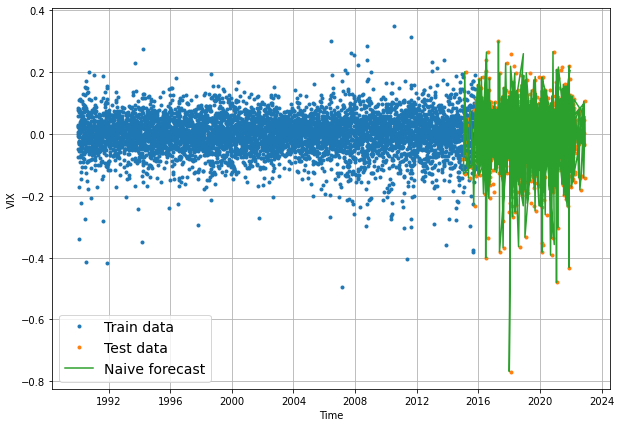
\includegraphics[width=4.92912in,height=3.3924in,keepaspectratio]{media/media/image29.png}
\caption{\emph{Na\"ive forecast} (source: [P4]).}
\label{fig:naive-forecast}
\end{figure}

% Figure 3.15
\begin{figure}[htbp]
\centering
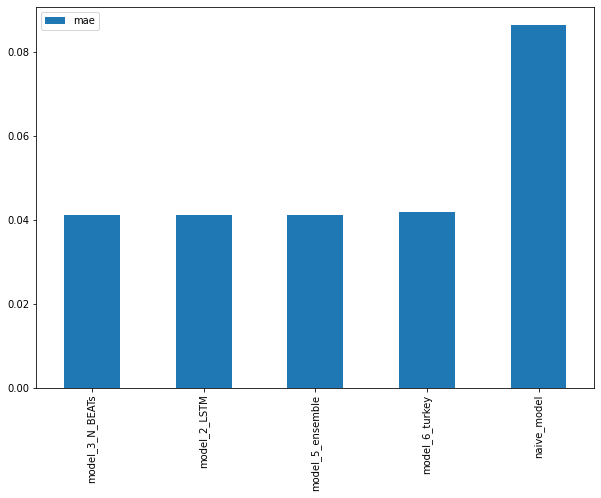
\includegraphics[width=4.7in,height=3.17431in,keepaspectratio]{media/media/image30.png}
\caption{Model performance (source: [P4]).}
\label{fig:3-29}
\end{figure}


The performance of all models was evaluated using MAE, MSE, RMSE and MASE metrics. Table 3.1 below summarizes the key findings.
% preamble (if not already)
% \usepackage{longtable}
% \usepackage{booktabs}
% \usepackage{array}

\begin{longtable}[]{@{}
  >{\raggedright\arraybackslash}p{(\columnwidth - 8\tabcolsep) * \real{0.3190}}
  >{\raggedright\arraybackslash}p{(\columnwidth - 8\tabcolsep) * \real{0.1703}}
  >{\raggedright\arraybackslash}p{(\columnwidth - 8\tabcolsep) * \real{0.1703}}
  >{\raggedright\arraybackslash}p{(\columnwidth - 8\tabcolsep) * \real{0.1703}}
  >{\raggedright\arraybackslash}p{(\columnwidth - 8\tabcolsep) * \real{0.1703}}@{}}

\caption{Performance metrics}\label{tab:performance-metrics}\\
\toprule
\textbf{Model} & \textbf{mae} & \textbf{mse} & \textbf{rmse} & \textbf{mase} \\
\midrule
\endfirsthead

\toprule
\textbf{Model} & \textbf{mae} & \textbf{mse} & \textbf{rmse} & \textbf{mase} \\
\midrule
\endhead

na\"ive\_model      & 0.0865 & 0.0153  & 0.0865 & 0.999 \\
model\_2\_LSTM      & 0.0412 & 0.00325 & 0.0570 & 0.672 \\
model\_3\_N\_BEATs  & 0.0411 & 0.00325 & 0.0570 & 0.671 \\
model\_5\_ensemble  & 0.0413 & 0.00327 & 0.0572 & 0.673 \\
model\_6\_turkey    & 0.0418 & 0.00342 & 0.0424 & 0.681 \\
\bottomrule
\end{longtable}




The results show that deep learning models like NBEATS (MAE: 0.0411) and
LSTM (MAE: 0.0412) significantly outperform the Naïve forecast (MAE:
0.0865). Furthermore, the hybrid GAN--SVM approach yielded a highly
competitive MAE of 0.004 and MAPE of 0.006, demonstrating the power of
using GANs for sophisticated feature generation. The NBEATS model
slightly outperforming LSTM with an MAE of 0.0412. This marginal
difference may reflect the ability of NBEATS to generalise over long
time horizons, whereas LSTM is better suited for capturing localised
patterns in high--frequency data. However, both models demonstrate strong
performance in identifying volatility trends, as evidenced by their MSE
values.

The empirical investigations presented in this chapter have served two
critical purposes in the overarching argument of this thesis. First, by
implementing and evaluating a wide array of models from classical
econometric methods like GARCH and ARIMA to advanced machine learning
techniques including LSTM, NBEATS, and GAN--SVM hybrids, we have
established a robust performance benchmark for existing volatility
forecasting methodologies. The results, detailed in
[P1], [P4] and summarised herein, demonstrate that while modern
machine learning models can achieve strong predictive accuracy, they
function primarily as sophisticated pattern--recognition systems. Their
architectural design does not inherently reflect the deep structural
properties of the data--generating process.

Second, and more fundamentally, this chapter provides the empirical
grounding for the central hypothesis of this thesis: that financial
volatility is a fractal phenomenon. The analysis of volatility
clustering using K--Means and Fuzzy C--Means revealed distinct, persistent
regimes that are not well--captured by models assuming simple random
walks. More formally, the calculation of the Hurst exponent for the VIX
time series consistently yielded values of H $\neq$ 0.5, confirming the
presence of long--range dependence and a ``rough`` character that defies
classical diffusion--based assumptions.

These findings, taken together, create a clear and compelling
justification for the theoretical work undertaken in the subsequent
chapters. While the models benchmarked in this chapter are powerful,
their limitations highlight a clear gap in the literature. To truly
advance our understanding and ability to model volatility, it is not
sufficient to apply ever--more--complex ``black box`` algorithms to the
data. It is necessary to develop a new theoretical framework, which is presented in Chapter 5, from first
principles that explicitly embeds the observed properties of fractality,
memory, and uncertainty into its core mathematical structure.

Therefore, the empirical results of this chapter serve as the essential
motivation for the development of the mixed fuzzy fractional Brownian
motion framework, which is the primary subject of Chapter 5.

\subsection{Conclusion}

This chapter has established the experimental and methodological foundations used throughout the empirical part of the thesis. We first motivated the use of recurrent deep learning for sequential financial data by outlining the Long Short--Term Memory (LSTM) architecture, its gating mechanism (input, forget, output), and the associated state dynamics in \eqref{eq:lstm-input-gate}--\eqref{eq:lstm-hidden-state}. Building on this, we specified a likelihood--based training objective for volatility forecasting, deriving the Gaussian log--likelihood in \eqref{eq:loglikelihood-normal} and adopting the corresponding negative log--likelihood loss in \eqref{eq:loss-sigma} to align model optimisation with probabilistic fit to observed returns.

We then discussed the vanishing--gradient phenomenon in recurrent training, highlighting how backpropagation through time (BPTT) produces multiplicative gradient chains \eqref{eq:grad-product} that can decay exponentially. The LSTM memory cell and gate structure were presented as the key architectural intervention that stabilises gradient flow via additive state updates and selective information retention, thereby improving learnability of long--horizon dependencies that are characteristic of volatility dynamics.

To ensure fair and leakage--free model comparison, the chapter introduced a standardised walk--forward validation design with rolling train--validation--test windows. Feature engineering was formalised via lagged returns, moving averages, and rolling volatility, while hyperparameter selection used grid search optimisation within each fold. This experimental protocol was applied consistently across classical baselines and modern architectures (LSTM, N--BEATS, GAN hybrids), enabling performance metrics to be aggregated across folds and interpreted as out--of--sample forecasting skill rather than artefacts of a single split.

A second major contribution of the chapter was the methodology for generating multifractal simulations under the Multifractal Model of Asset Returns (MMAR). We defined multifractality via scaling of moments \eqref{eq:3.1.5}, constructed partition functions \eqref{eq:3.1.6}, estimated the scaling function $\tau(q)$ via log--linear regression \eqref{eq:3.1.7}, and obtained the Hurst exponent through the root condition \eqref{eq:3.1.8}--\eqref{eq:3.1.9}. The multifractal spectrum was then recovered through a Legendre transform \eqref{eq:3.1.10}, allowing estimation of the most probable H\"older exponent \eqref{eq:3.1.11} and the cascade parameters $\lambda$ and $\sigma^2$ in \eqref{eq:3.1.12}--\eqref{eq:3.1.13}. These parameters support simulation of a lognormal multiplicative cascade and its cumulative trading time $\theta(t)$ \eqref{eq:3.1.14}, which is subsequently time--changed through fractional Brownian motion \eqref{eq:3.1.15} to produce the composite MMAR process $X_t = B_H\!\big[\Theta(t)\big]$. The chapter also reviewed long--range dependence testing via the rescaled range statistic \eqref{eq:RS_n-ch3}--\eqref{eq:RS_log_linear-ch3}, empirically illustrating the contrast between persistent behaviour in long--horizon equity indices and stronger mean reversion in volatility, consistent with volatility clustering and regime shifts.

Finally, the chapter connected these methodological elements to empirical benchmarking. Volatility regimes were identified via K--Means and Fuzzy C--Means clustering, with silhouette--based model selection and transition--matrix asymmetries providing evidence of non--uniform regime switching and jump--like behaviour. Forecasting benchmarks spanning naive methods, ARIMA, deep networks, and hybrid GAN--SVM/RF pipelines were then summarised, clarifying that discriminator accuracy reflects adversarial training dynamics rather than forecast skill, and emphasising that model evaluation must rely on out--of--sample error metrics. Collectively, these results motivate the thesis perspective that strong predictive performance alone is insufficient: volatility exhibits memory, fractality, and regime structure that warrant explicit modelling assumptions rather than purely black--box pattern recognition.

In summary, this chapter delivers (i) a reproducible experimental design for robust comparison of machine learning forecasters, and (ii) a principled multifractal simulation pipeline capable of generating long--memory, clustered--volatility synthetic data. These foundations provide the empirical motivation and computational apparatus required for the subsequent theoretical development, where the thesis advances a modelling framework that embeds fractality, memory, and uncertainty directly into the underlying stochastic structure.

\hypertarget{chapter--4--evaluation--metrics}{%
\chapter{\texorpdfstring{\textbf{CHAPTER 4 -- EVALUATION
METRICS}}{CHAPTER 4 ---- EVALUATION METRICS}}\label{chapter--4--evaluation--metrics}}

\hypertarget{introduction--2}{%
\section{\texorpdfstring{\textbf{
INTRODUCTION}}{INTRODUCTION}}\label{introduction--2}}

Evaluation metrics are fundamental tools for assessing the performance
of predictive models. This chapter focuses on three widely used metrics:
Root Mean Squared Error (RMSE), Mean Absolute Error (MAE), and Mean
Absolute Percentage Error (MAPE). These metrics quantify prediction
accuracy by comparing predicted values against observed data. While this
chapter does not present novel evaluation metrics, it provides a
detailed exploration of these standard measures, highlighting their
strengths, limitations, and applications.

\hypertarget{root--mean--squared--error}{%
\section{\texorpdfstring{\textbf{ROOT MEAN SQUARED
ERROR}}{ROOT MEAN SQUARED ERROR}}\label{root--mean--squared--error}}

Root mean squared error (RMSE) \cite{moody2019what_73} or root mean square deviation is
one of the most used metrics to assess the quality of a forecast. It
shows how far the predictions deviate from the actual values
\hspace{0pt}\hspace{0pt}measured using the Euclidean distance. RMSE is
commonly used in supervised learning applications because the RMSE uses
and requires real measurements at each predicted data point.

RMSE is the square root of the mean of the square of all the errors. The
use of RMSE is very common and is considered an excellent
general--purpose measure of error for numerical predictions.

\begin{equation}\label{eq:4.1.1}
\mathrm{RMSE}
= \sqrt{\frac{1}{n}\sum_{i=1}^{n}\bigl(S_i - O_i\bigr)^{2}} \, .
\end{equation}

where Oi are the observations, Si predicted values of a variable, and n
the number of observations available for analysis. RMSE is a good
measure of accuracy, but only for comparing the prediction errors of
different models or model configurations for a particular variable and
not between variables, as it is scale dependent.

4.2.2 is a restatement of 4.2.1 but uses different notations for
predicted and observed values. It emphasises the normalisation step by
n, which ensures that RMSE reflects the average error magnitude rather
than a cumulative measure. This normalisation is critical for datasets
with varying sizes, as it provides a consistent scale for comparison. To
calculate RMSE, compute the difference between prediction and actual for
each data point, calculate the norm of residual for each data point,
compute the mean of residuals and take the square root of this average.

\begin{equation}\label{eq:4.1.1}
\mathrm{RMSE}
= \sqrt{\frac{1}{n}\sum_{i=1}^{n}\bigl(S_i - O_i\bigr)^{2}}.
\end{equation}


where n is the number of observations, y(i) is the observed value, and
$\hat{y}$(i) is its predicted value.

4.2.3 introduces the use of a norm (||$\cdot$||) for computing residuals,
connecting RMSE to broader mathematical contexts such as vector norms.
The use of norms highlights RMSE's interpretation as a Euclidean
distance between predicted and observed values in $\mathbb{R}$\textsuperscript{n}. This
interpretation is especially relevant for geometric or spatial data
where distances are meaningful.

\begin{equation}\label{eq:4.1.3}
\mathrm{RMSE}
= \frac{1}{\sqrt{n}}\left\lVert y-\widehat{y}\right\rVert_2 .
\end{equation}



where \emph{N} is the number of data points, \emph{y(i)} is the i--th
measurement, and \emph{$\hat{y}$(i)} is its corresponding prediction.

By squaring errors and calculating a mean, the RMSE can be strongly
influenced by some predictions much worse than others. If this is
undesirable, using the absolute value of residuals and/or calculating
median can provide a better idea of how a model performs for most
predictions, without further influence from the anomalously poor
predictions.

In machine learning, RMSE is a single number that is extremely useful
for evaluating a model's performance, whether during training,
cross--validation, or post--deployment monitoring. It is a proper scoring
rule that is intuitive to understand and compatible with some of the
most common statistical assumptions.

From a mathematical perspective and ignoring the division by n under the
square root, the first thing we can notice is a resemblance to the
formula for the Euclidean distance between two vectors in \emph{$\mathbb{R}$\textsuperscript{n}}:

\begin{equation}\label{eq:4.1.4}
\operatorname{dist}(x,y)
= \sqrt{\sum_{i=1}^{n}\bigl(x_i-y_i\bigr)^2}.
\end{equation}


This tells us heuristically that RMSE can be thought of as some kind of
(normalized) distance between the vector of predicted values and the
vector of observed values.

If we keep the number of observations fixed as \emph{n}, all it does is
rescale the Euclidean distance by a factor of \emph{$\sqrt{}$(1/n).} If we
assume that our observed values are determined by adding random
``errors'' to each of the predicted values, we obtain as follows:

{\centering
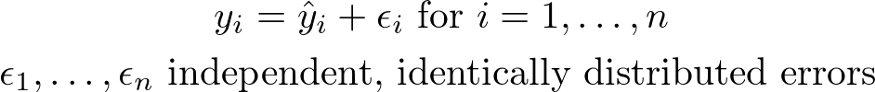
\includegraphics[width=4.30208in,height=0.39583in,keepaspectratio]{media/media/image33.png}\par
}
These errors are random variables and might have Gaussian distribution
with mean \emph{$\mu$} and standard deviation \emph{$\sigma$}, but any other
distribution with a square--integrable probability density function would
also work. We want to think of \emph{$\hat{y}$\textsubscript{i}} as an underlying physical
quantity, such as the exact distance from \emph{A} to \emph{B} at a
particular point in time. Our observed quantity \emph{y\textsubscript{i}} would then be
the distance from \emph{A} to the \emph{B} as we measure it, with some
errors coming from mis--calibration of our measure tool and measurement
noise from external interference.

The mean \emph{$\mu$} of the distribution of our errors will correspond to
the continuous bias that comes from poor calibration, while the standard
deviation \emph{$\sigma$} would correspond to the amount of measurement noise.
Now imagine that we know the mean \emph{$\mu$} of the distribution for our
errors exactly and would like to estimate the standard deviation
\emph{$\sigma$}. We can see that:

\begin{equation}\label{eq:4.1.5}
\begin{aligned}
\mathbb{E}\!\left[\frac{1}{n}\sum_{i=1}^{n}\bigl(\widehat{y}_i-y_i\bigr)^{2}\right]
&= \mathbb{E}\!\left[\frac{1}{n}\sum_{i=1}^{n}\varepsilon_i^{2}\right] \\
&= \frac{1}{n}\sum_{i=1}^{n}\mathbb{E}\!\left[\varepsilon_i^{2}\right] \\
&= \mathbb{E}\!\left[\varepsilon^{2}\right] \\
&= \operatorname{Var}(\varepsilon)+\bigl(\mathbb{E}[\varepsilon]\bigr)^{2} \\
&= \sigma^{2}+\mu^{2}.
\end{aligned}
\end{equation}


Here \emph{E{[}\ldots{]}} is the expectation, and \emph{Var(\ldots)} is
the variance. We can replace the mean of the expectations
\emph{E{[}$\epsilon$\textsubscript{i}\textsuperscript{2}{]}} with the \emph{E{[}$\epsilon$\textsuperscript{2}{]}} where \emph{$\epsilon$} is a variable
with the same distribution as each of the \emph{$\epsilon$}\textsubscript{i}, because the errors
$\epsilon$\textsubscript{i} are identically distributed, and thus their squares all have the same
expectation.

We assumed that we already knew \emph{$\mu$} exactly. In other words, the
persistent bias in our instruments is a known bias, rather than an
unknown bias. So, we can also correct this bias from the start by
subtracting $\mu$ from all our raw observations. That is, we can also assume
that our errors have been distributed with mean \emph{$\mu$ = 0.} Plugging
this into the equation above and taking the square root of both sides
then yields:

\begin{equation}\label{eq:4.1.6}
\sqrt{\mathbb{E}\!\left[\frac{1}{n}\sum_{i=1}^{n}\bigl(\widehat{y}_i-y_i\bigr)^{2}\right]}
= \sqrt{\sigma^{2}+0^{2}}
= \sigma .
\end{equation}

If we removed the expectation \emph{E{[} \ldots{} {]}} from inside the
square root, it is exactly our formula for RMSE from before if the
errors are unbiased (\emph{$\mu$=0}). The Central Limit Theorem tells us
that as n increases, the variance of the quantity \emph{$\Sigma$\textsubscript{i} ($\hat{y}$\textsubscript{i} --- y\textsubscript{i})\textsuperscript{2}
/ n = $\Sigma$\textsubscript{i} ($\varepsilon$\textsubscript{i})\textsuperscript{2} / n} should converge to zero. In fact, a more robust form
of the central limit theorem tells us its variance should converge to 0
asymptotically like \emph{1/n.} This tells us that \emph{$\Sigma$\textsubscript{i} ($\hat{y}$\textsubscript{i} --- y\textsubscript{i})\textsuperscript{2}
/ n} is a good estimator for \emph{E{[}$\Sigma$\textsubscript{i} ($\hat{y}$\textsubscript{i} --- y\textsubscript{i})\textsuperscript{2} / n{]} = $\sigma^2$.} But
then the RMSE is a good estimator of the standard deviation \emph{$\sigma$} of
our error distribution. We should also now have an explanation for
division by n under the square root of the RMSE. It allows us to
estimate the standard deviation \emph{$\sigma$} of the error for a typical
single observation rather than some kind of ``total error''. By dividing
by \emph{n}, we keep this measure of error consistent as we move from a
small collection of observations to a larger collection, and it just
becomes more accurate as we increase the number of observations. To
paraphrase it another way, RMSE is a good way to answer the question:
``\emph{How far off should we expect our model to be on its next
prediction?}''

RMSE is a good measure to use if we want to estimate the standard
deviation $\sigma$ of a typical observed value from our model's prediction,
assuming that our observed data can be decomposed in accordance with
Doob's theorem:

\emph{Observed value= predicted value + predictably distributed random
noise with mean zero}

There is a limitation here which is that Doob's theorem requires that
the stochastic process be a semimartingale but the fBm processes we are
modelling are neither a semimartingale nor a weak martingale. It is a
Gaussian process with stationary increments, but its sample paths are
not of finite variation and its increments are not orthogonal to the
past. Recently a concept of fractional semimartingale has gained
traction but there is no consensus on the definition and the concept is
still under development. The random noise here could be anything that
our model does not capture (e.g., unknown variables that might influence
the observed values). If the noise is small, as estimated by the RMSE,
it generally means that our model predicts our observed data well, and
if the RMSE is large, it usually means that our model does not consider
important features located in our data. In machine learning and this
paper, RMSE has a double purpose to serve as a heuristic for training
models and to evaluate trained models for usefulness and accuracy. This
raises an important question: What does it mean for RMSE to be `small'?
Firstly, ``small'' will depend on our choice of unit and the application
we want. For training models, it doesn't matter which unit we use,
because all we care about during training is having a heuristic to help
us reduce the error at each iteration. We are only interested in the
relative size of the error from one step to the next, not the absolute
size of the error.

But in evaluating trained models in data science for usefulness and
accuracy, we do care about units, because we aren't just trying to see
if we're doing better than last time: we want to know if our model can
help us solve a practical problem. The nuance here is that judging
whether the RMSE is small enough will depend on how precise we need our
model for our given application. There is never going to be a
mathematical formula for this because it depends on things like human
intentions i.e., purpose of the model, and risk aversion such as how
much harm would be caused if this model made an inaccurate prediction.
In other words, our choice of machine learning model (e.g., SVM, LSTM,
naïve Bayes) and RMSE for predicting cancer or heart attack will be very
different to the models and RMSE used for predicting stock market
changes. Equally, the social and ethical considerations of the magnitude
of errors resulting from self--driving \emph{Uber} cars or facial
recognition software are quite different to the social impact coming
from errors in \emph{Youtube} algorithm or routine \emph{satnav}
algorithms.

Besides the units, there is also another consideration: `small' also
needs to be measured relative to the type of model being used, the
number of data points, and the history of training the model went
through before you evaluated it for accuracy. At first this may sound
counter--intuitive, but not when you consider the problem of
over--fitting.

There is a risk of overfitting whenever the number of parameters in your
model is large relative to the number of data points you have. For
example, if we are trying to predict one real quantity \emph{y} as a
function of another real quantity \emph{x}, and our observations are
\emph{(x\textsubscript{i}, y\textsubscript{i})} with \emph{x\textsubscript{1} \textless{} x\textsubscript{2} \textless{} x\textsubscript{3} \ldots{}
\textless{} x(n)}, a general interpolation theorem tells us there is
some polynomial \emph{f(x}) of degree at most \emph{n+1} with
\emph{f(x\textsubscript{i}) = y\textsubscript{i} for i = 1, \ldots{} , n.} This means that if we choose
our model to be a polynomial of order \emph{n + 1}, by adjusting the
parameters of the model (the polynomial coefficients) we should be able
to bring the RMSE down to 0. This is true regardless of what our y
values are. In this case the RMSE tells us nothing about the accuracy of
our underlying model. We have been assured that we can modify the
parameters to get RMSE=0 as measured on our existing data points,
whether there is a relationship between two real quantities or not.

But it's not only when the number of parameters exceeds the number of
data points that we might run into problems. Even if we don't have an
unreasonable number of parameters, it is still possible that general
mathematical principles along with moderate assumptions about our data
may guarantee us with a high probability that by adjusting the
parameters of the model, we can bring the RMSE below a certain
threshold. If we are in such a situation, the fact that the RMSE was
below this threshold might not say anything significantly about the
predictive power of our model. Statistically speaking, the question we
are going to be asking is not whether RMSE of our trained model is small
but rather, what is the probability that the RMSE of our trained model
on these observations is this small by a random chance.

\hypertarget{mean--absolute--error--mae}{%
\section{\texorpdfstring{\textbf{MEAN ABSOLUTE ERROR
(MAE)}}{MEAN ABSOLUTE ERROR (MAE)}}\label{mean--absolute--error--mae}}

Mean Absolute Error (MAE) \cite{willmott2005advantages_74} measures the average magnitude of
errors between paired observations for the same variable. It is commonly
used to evaluate prediction accuracy in time series analysis, regression
tasks, and other contexts where interpretability is important. Examples
include comparing predicted values to observed values, measuring changes
between baseline and follow--up, or assessing differences between two
measurement techniques.

MAE is calculated as:

\begin{equation}\label{eq:4.1.7}
\mathrm{MAE}
= \frac{1}{n}\sum_{i=1}^{n}\left|y_i-\widehat{y}_i\right|
= \frac{1}{n}\sum_{i=1}^{n}\left|e_i\right|.
\end{equation}


It is an arithmetic average of the absolute error
\emph{\textbar e\textsubscript{i}\textbar=\textbar y\textsubscript{i} ----
x\textsubscript{i}\textbar,} where \emph{y\textsubscript{i}} is the
prediction and \emph{x\textsubscript{i}} is the true value. Other
formulations may include relative frequencies as weight factors. One of
MAE's key advantages is its robustness to outliers compared to metrics
that square errors, such as Root Mean Squared Error (RMSE). However, MAE
is scale--dependent, meaning it cannot be used to compare error
magnitudes across datasets with different units or scales. This
limitation should be considered when selecting MAE as an evaluation
metric.

\hypertarget{mean--absolute--percentage--error}{%
\section{\texorpdfstring{\textbf{MEAN ABSOLUTE PERCENTAGE
ERROR}}{MEAN ABSOLUTE PERCENTAGE ERROR}}\label{mean--absolute--percentage--error}}

Mean absolute percentage error (MAPE) also known as regression loss is
added to all the models along with RMSE and MAE. MAPE's best value is
0.0 and inaccurate predictions can lead to arbitrarily large MAPE
values, especially if some y\_true values are very close to zero. This
function returns undefined value of infinity when y\_true is zero
because division by zero is not defined. Here is an actual formula.

\begin{equation}\label{eq:4.1.8}
\mathrm{MAPE}
= \frac{100\%}{n}\sum_{t=1}^{n}\left|\frac{A_t - F_t}{A_t}\right|.
\end{equation}

where~\emph{A\textsubscript{t~}}is the actual value
and~\emph{F\textsubscript{t}}~is the forecast value. Their difference is
divided by the actual value~\emph{A\textsubscript{t}}. The absolute
value in this ratio is added for each prediction time point and divided
by the number of adjusted points~n.

\hypertarget{conclusion}{%
\section{\texorpdfstring{\emph{\textbf{CONCLUSION}}}{CONCLUSION}}\label{conclusion}}

This chapter has presented the evaluation criteria used throughout the empirical studies of the thesis, focusing on three standard point--forecast error measures: RMSE, MAE, and MAPE. We defined each metric formally and clarified the distinct loss geometries they induce. RMSE, as an $\ell_2$ measure, penalises large deviations quadratically and is therefore highly sensitive to outliers; it can be interpreted as a (normalised) Euclidean distance between the vectors of predictions and observations and, under unbiased square--integrable error assumptions, relates to the typical dispersion of the residuals. MAE, as an $\ell_1$ measure, provides a more robust summary of typical error magnitude by reducing the influence of extreme residuals, at the cost of being less sensitive to rare but economically important tail events. MAPE offers a scale--free percentage interpretation that can be convenient for cross--series comparison, but it is unstable when realised values are close to zero and is undefined at zero, which limits its suitability for return series or other data with near--zero denominators.

Beyond definitions, the chapter has emphasised that the meaning of a ``small'' error is application--dependent and that metric choice should be consistent with the decision problem (e.g., tail risk sensitivity versus typical accuracy) and with the data scale. The discussion also highlighted that low in--sample errors can be misleading in high--capacity models due to overfitting, reinforcing the need for out--of--sample evaluation and appropriate validation protocols when comparing forecasting approaches.

Finally, we noted an important modelling nuance that motivates later chapters: many common interpretations of squared--error criteria are rooted in classical semimartingale diffusion settings and independence assumptions, whereas the volatility processes considered in this thesis may exhibit long--range dependence and roughness (e.g., fractional Brownian components). While RMSE/MAE/MAPE remain useful as practical, model--agnostic scoring rules for benchmark comparisons, their limitations underscore the importance of pairing them with careful experimental design and with diagnostics that reflect dependence structure and scaling behaviour. Taken together, the metrics formalised here provide a transparent and consistent basis for evaluating the forecasting models developed and benchmarked in subsequent chapters.

Accordingly, RMSE, MAE and, where numerically appropriate, MAPE, are used as the primary scoring rules for the comparative experiments in later chapters, supplemented by dependence- and scale-aware diagnostics when assessing models designed to capture long-memory or rough dynamics.


\hypertarget{chapter--5--mixed--fuzzy--fractional--brownian--motion--with--jumps}{%
\chapter{\texorpdfstring{\textbf{CHAPTER 5 -- MIXED FUZZY FRACTIONAL
BROWNIAN MOTION WITH
JUMPS}}{CHAPTER 5 ---- MIXED FUZZY FRACTIONAL BROWNIAN MOTION WITH JUMPS}}\label{chapter--5--mixed--fuzzy--fractional--brownian--motion--with--jumps}}

\hypertarget{fuzzy--fractional--brownian--motion}{%
\section{\texorpdfstring{\emph{\textbf{FUZZY FRACTIONAL BROWNIAN
MOTION}}}{FUZZY FRACTIONAL BROWNIAN MOTION}}\label{fuzzy--fractional--brownian--motion}}

In the field of stochastic process modelling, the fractional Brownian
motion (fBm) is often recommended as a replacement for Brownian motion
as the driving process, particularly when studying phenomena
characterised by long--range dependence. The fBm, with a Hurst exponent
(\emph{H}) ranging between 0 and 1, is a type of Gaussian process that
possesses several advantageous properties, including long--range
dependence, self--similarity, and stationarity of increments. Notably,
when the Hurst exponent is different from 1/2, the fBm ceases to be a
semi--martingale. This chapter is somewhat reliant on an earlier work of
Doob--Meyer decomposition theorem which provides a representation of a
submartingale as the sum of a martingale and an increasing predictable
process. This theorem lays foundation for the decomposition of
submartingales into their components. If we let \emph{X(t)} be a
submartingale with respect to a filtration (a sequence of sigma
algebras), then there exists a unique, increasing, predictable process
\emph{A(t)} such that the martingale process \emph{M(t)} can be defined
as \emph{M(t) = X(t) ---- A(t)}. In other words, according to Doob--Meyer
the submartingale can be decomposed into the sum of a martingale
\emph{M(t)} and an increasing predictable process \emph{A(t).} The proof
for a continuous case is very complicated and can be found in \cite{meyer1962decomposition_75}.
However, there is a contradiction here as it was said that the fBM is
not even a semi--martingale.

In [P2] we proposed to review and extend proofs in mixed fuzzy
stochastic Brownian motion as novel equations suitable for modelling
hybrid systems. These equations provide a flexible framework that can
effectively capture the dynamics of complex systems characterized by
both stochastic and fuzzy components. By combining the concepts of fuzzy
logic and stochastic processes, we aim to address the modelling
challenges associated with hybrid systems. Applications of these
processes can be made in the telecommunication industry, where
measurements of variables suffer from latency and financial industry,
where participants are operating under uncertainty.

To illustrate the applicability of our approach, we utilise the
Liouville form of the fractional Brownian motion. The Liouville form
represents a particular representation of the fBm that allows for an
enhanced analysis and interpretation of its properties. By leveraging
this form, we can gain further insights into the behaviour of the mixed
fuzzy stochastic Brownian motion, thereby facilitating their use in a
wide range of modelling scenarios.

In summary, this paper proposes the utilisation of the mixed fuzzy fBm
as a replacement for Brownian motion in stochastic process modelling,
specifically focusing on its advantageous properties such as long--range
dependence, self--similarity, and stationarity of increments.
Furthermore, we introduce proofs and extensions for some novel
equations, namely the mixed fuzzy stochastic Brownian motion with jumps,
to address the modelling needs of hybrid systems.

\hypertarget{preliminaries}{%
\subsection{\texorpdfstring{PRELIMINARIES
}{PRELIMINARIES }}\label{preliminaries}}

In this section, the fundamental mathematical definitions and notations that underpin the theoretical framework of this chapter are established. The stochastic basis on which the asset price and volatility processes are constructed is defined as follows. Let $(\Omega, \mathcal{F}, \mathbb{P})$ be a complete probability space equipped with a natural filtration $\mathbb{F} = \{\mathcal{F}_t\}_{t \geq 0}$ satisfying the usual conditions of right--continuity and completeness. This filtration represents the information set available to market participants at any time $t$, encompassing both the continuous market evolution and discontinuous jump events.

Central to the modelling approach is the concept of Fractional Brownian Motion (fBm), which serves as the primary stochastic driver for the underlying asset dynamics. A standard fractional Brownian motion $B^H = \{B^H_t, t \geq 0\}$ with Hurst parameter $H \in (0, 1)$ is defined as a continuous Gaussian process with zero mean, $B^H_0 = 0$, and the covariance function $\mathbb{E}[B^H_t B^H_s] = \frac{1}{2}(t^{2H} + s^{2H} - |t-s|^{2H})$. This process generalises standard Brownian motion (obtained when $H = \frac{1}{2}$), providing the necessary mathematical flexibility to capture the self--similarity and long--range dependence ($H > \frac{1}{2}$) or anti--persistence ($H < \frac{1}{2}$) observed in the volatility time series analysed in the preceding chapters.

Building upon these foundational concepts, the specific stochastic process utilised in this framework is defined below.

\textbf{Definition (Mixed Multifractal Fuzzy Fractional Brownian Motion -- mmffBm)}

The Mixed Multifractal Fuzzy Fractional Brownian Motion (mmffBm) is defined as a generalized stochastic process operating within a fuzzy probability space. It is constructed as a superposition of a standard Brownian motion $W(t)$ and an independent fractional Brownian motion $B^H(t)$, governed by fuzzy coefficients.

The continuous process $M^H(t, \tilde{\xi})$ is defined by:
\begin{equation}
    M^H(t, \tilde{\xi}) = \tilde{a} W(t) + \tilde{b} B^H(t), \quad t \ge 0,
\end{equation}
where:
\begin{itemize}
    \item $W(t)$ is a standard Brownian motion (Hurst parameter $H = \frac{1}{2}$).
    \item $B^H(t)$ is an independent fractional Brownian motion with Hurst parameter $H \in (0, 1)$ and $H \neq \frac{1}{2}$.
    \item $\tilde{a}$ and $\tilde{b}$ represent fuzzy numbers characterizing the weights of the standard and fractional components, respectively.
\end{itemize}

This mixed structure allows the process to exhibit properties of both semimartingales (via $W(t)$) and long--memory processes (via $B^H(t)$). Furthermore, the combination of distinct Hurst exponents ($0.5$ and $H$) results in a process with time--varying local regularity, satisfying the condition for multifractality. This framework is specifically designed to derive results for regimes where $H > \frac{1}{2}$ (persistence) and $H < \frac{1}{2}$ (anti--persistence) under conditions of fuzzy uncertainty.
\hypertarget{fractional--brownian--motion}{%
\subsection{FRACTIONAL BROWNIAN
MOTION}\label{fractional--brownian--motion}}

The fBm BH is a zero mean Gaussian process with the following
covariance function:

\begin{equation}\label{eq:5.1.1}
C_{B^{H}}(t,s)
=\mathbb{E}\!\left[B_{H}(t)\,B_{H}(s)\right]
=\frac{1}{2}\left(t^{2H}+s^{2H}-|t-s|^{2H}\right), \qquad s,t\ge 0.
\end{equation}

This was derived in Kolmogorov \cite{kolmogorov1940wienersche_76} and further studied in
Mandelbrot and van Ness \cite{ness1968fractional_4}, where a stochastic integral
representation was derived in terms of the Brownian motion ---- see
equation 3.5.14. \(\int_{0}^{t}{\lbrack(t - s)^{H - \frac{1}{2}}\rbrack dB(s))}\) is
called the Liouville form of a fBm and it holds many properties of the
fBm except that it has non--stationary increments. The classical Itô
theory cannot handle a stochastic integral in terms of fBm because
B\textsuperscript{H} is not a semi--martingale if \emph{H $\neq$ $\frac{1}{2}$.} Two
approaches have been used to evaluate stochastic integrals with respect
to fBm. If \emph{H\textgreater{} 1/2}, the Riemann--Stieltjes stochastic
integral can be defined using Young's integral \cite{young1936inequality_77}.

Suppose we have a financial time series representing the price of a
stock over a certain period of time, denoted by \emph{S(t).} We want to
calculate the Riemann--Stieltjes stochastic integral of the stock price
with respect to a cumulative trading volume, denoted by \emph{V(t),}
which represents the total number of shares traded up to time \emph{t.}

\begin{enumerate}
    \item \text{Partition:} Choose a partition of the time interval into subintervals. For simplicity, consider a uniform partition with $n$ subintervals.

    \item \text{Piecewise Linear Approximation:} Approximate $V(t)$ on each subinterval using a piecewise linear function. This can be achieved by interpolating the cumulative trading volume between the available data points.

    \item \text{Young's Integral Calculation:} Calculate the Riemann--Stieltjes integral using Young's integral approach.
    \begin{enumerate}
        \item For each subinterval, compute the integral of $S(t)$ with respect to the piecewise linear approximation of $V(t)$.
        \item This operation is performed by multiplying the stock price at each subinterval by the change in the approximated cumulative trading volume.
    \end{enumerate}

    \item \text{Refinement and Convergence:} Repeat the above steps with increasingly finer partitions.
    \begin{enumerate}
        \item Refine the piecewise linear approximation of $V(t)$ at each step.
        \item Recalculate the Riemann--Stieltjes stochastic integral using Young's integral.
        \item By repeating this process, the integral will converge to a well--defined value, representing the integral of the stock price with respect to the cumulative trading volume over the given time period.
    \end{enumerate}
\end{enumerate}

This methodology provides insights into the relationship between trading activity and stock price movements.
In practice, to define \(\int_{}^{}{S(t)}\, dV(t)\) via a
Riemann----Stieltjes/Young framework, one partitions \emph{{[}0,T{]}} into
\(0 = t_{0} < t_{1} < \cdots < t_{n} = T\), uses piecewise
approximations of \emph{V}, and sums
\(S(t_{i})\lbrack V(t_{i + 1}) - V(t_{i})\rbrack.\ \)One refines this
partition to ensure convergence. For \emph{H \textgreater{}
$\frac{1}{2}$}\hspace{0pt}, fBm has sample paths of sufficient Hölder regularity to
admit such an integral.

The general obstruction to using the classical
Riemann--Stieltjes or Lebesgue--Stieltjes integral with
\emph{B\textsuperscript{H}} is fBm paths are not of bounded variation
(a.s.) for any \emph{H} \(\epsilon\) (0,1) and even Brownian motion does
not have bounded variation. This makes the Young's integral more
flexible and easier to use in stochastics. The Riemann--Stieltjes
integral cannot be used to define an integral of a function with respect
to fBm, because the Stieltjes measure is \emph{sometimes} not defined
for stochastic processes with non--stationary increments like fBm. A
Stieltjes measure is a generalisation of the Lebesgue measure to allow
for integration over sets with irregular boundaries. A Stieltjes measure
is defined on a measurable space (\emph{X, A}), where \emph{X} is a set
and \emph{A} is a $\sigma$--algebra of subsets of \emph{X}. A Stieltjes measure
is a function \emph{$\mu$}: \emph{A $\rightarrow$ {[}0, $\infty${]}} that satisfies the
following properties:

\begin{enumerate}
\def\labelenumi{\roman{enumi}.}
\item
  \emph{$\mu$($\emptyset$) = 0}.
\item \emph{Finite Additivity:} $\mu(A \cup B) = \mu(A) + \mu(B)$ for all disjoint sets $A, B \in \mathcal{A}$.
\item
  If \emph{A\_1 $\subset$ A\_2 $\subset$} $\cdots$ is a sequence of sets in \emph{A} such that
  \emph{A\_n $\uparrow$ A}, then \emph{$\mu$(A) = lim\_n$\rightarrow$$\infty$ $\mu$(A\_n).}
\end{enumerate}

The third property is called the continuity property. It ensures that
the Stieltjes measure is not sensitive to small changes in the sets that
are being measured. Stieltjes measures can be used to define integrals
of functions with respect to sets with irregular boundaries. For
example, the Stieltjes measure can be used to define the integral of a
function with respect to a Cantor set. These are fractal sets that are
constructed by repeatedly removing a middle third of a line segment.
Cantor sets have no Lebesgue measure, but they do have a Stieltjes
measure. This means that we can define the integral of a function with
respect to a Cantor set. Here is an example of how to use a Stieltjes
measure to define the integral of a function with respect to a set with
an irregular boundary:

Let \emph{X = {[}0, 1{]}} and let \emph{A} be the $\sigma$--algebra of all Borel
subsets of \emph{X}. Let \emph{g(t)} be the Cantor function. The Cantor
function is a continuous function that is defined on the interval {[}0,
1{]} and has the following properties:

\begin{enumerate}
\def\labelenumi{\roman{enumi}.}
\item
  \emph{g(0) =0} and \emph{g(1) = 1}.
\item
  \emph{g(t)} is constant on each interval of the form \emph{{[}a,
  b{]},} where \emph{a} and \emph{b} are points of the Cantor set.
\item
  The value of \emph{g(t)} on each interval of the form \emph{{[}a,
  b{]}} is equal to the average of the values of \emph{g(a)} and
  \emph{g(b).}
\end{enumerate}

The Cantor function is a pathological function, which means it has some
unusual features. The Cantor function \emph{g}: {[}0,1{]}$\rightarrow$ {[}0,1{]}
(sometimes called the Devil's staircase) is the classic example of a
continuous, non--decreasing function that is constant on the intervals
removed in constructing the Cantor set and increases from \emph{g(0)=0}
to \emph{g(1)=1}. It is a set of points that are sparse but not empty.
Despite the Cantor set having Lebesgue measure zero, the function
\emph{g} induces a nontrivial Stieltjes measure
\emph{$\mu$\textsubscript{g}} defined by:

\[\mu_{g}((a,b\rbrack) = g(b) - g(a),\]

\[\mu(A)\  = \ g(b)\  - \ g(a),\]

where \emph{A} is a Borel subset of \emph{X} and \emph{{[}a, b{]}} is
the smallest interval of the form \emph{{[}a, b{]}} that contains
\emph{A} which itself must be an interval. We can now use the Stieltjes
measure to define the integral of a function \emph{f(t)} with respect to
the Cantor function \emph{g}:

\[
\int_{0}^{1} f(t)\,\mathrm{d}g(t)
= \int_{[0,1]} f(t)\,\mathrm{d}\mu_{g}(t),
\]


where: \emph{f(t)} is the function that we want to integrate;
\emph{g(t)} is the Cantor function or the cdf corresponding to the pdf ;
\emph{$\mu$} is the Stieltjes measure induced by \emph{g}.


The measure \emph{$\mu$\textsubscript{g}}\hspace{0pt} is singular with
respect to Lebesgue measure: it is supported on the Cantor set (which
has Lebesgue measure 0) and assigns it total mass 1. This integral is
defined for all functions \emph{f(t)} that are measurable with respect
to the Lebesgue measure. The Cantor set has Lebesgue measure 0, but we can still define the
Stieltjes measure for the Cantor set with respect to g. This is because the Stieltjes measure is a more
general measure than the Lebesgue measure. This illustrates that
Stieltjes measures can assign positive measure to sets (like the Cantor
set) that have Lebesgue measure zero.

The Lebesgue measure is a measure that is defined on the Borel sets of
the real line. The Borel sets of the real line are the sets that can be
formed from the open sets of the real line using the operations of
countable union, countable intersection, and complementation. The
Stieltjes measure is a measure that is defined on the Borel sets of the
real line.
When we define the Stieltjes measure for the absolutely continuous
function such as probability density function, or for the Cantor
function, we are using the Borel \emph{$\sigma$}--\emph{algebra} (the same
domain as Lebesgue measure) to define the sets on which the Stieltjes
measure is defined on. However, we are not using the Lebesgue measure to
define the values of the Stieltjes measure. The values of the Stieltjes
measure are defined by the probability density function or the Cantor
function. The Stieltjes measure for the Cantor function or for a pdf can
be used to define the integral of a function with respect to that
function. 

The integral of a function with respect to the Cantor function can be
used to calculate the area under the graph of the Cantor function. This
does not equal the geometric  area under the graph of \emph{g},
which equals $\frac{1}{2}$. Moreover, while Young's integral provides a pathwise
calculus suitable for rough integrators such as fBm with H
\textgreater{} $\frac{1}{2}$, Lebesgue ---- Stieltjes measures are measure--theoretic
device built from distribution functions such as the Cantor function
and, in the Cantor case, yield the Cantor (Lebesgue-- Stieltjes) measure,
which assigns total mass of 1 to the Cantor set.

In summary, both Young's integral and Stieltjes measures are valuable
mathematical tools, but their applicability depends on the
characteristics of the stochastic process being studied and the
mathematical framework in which they are used. Young's integral is
tailored to the needs of fBm and related processes, while Stieltjes
measures are more general and can be applied to a wider range of
scenarios.

If \emph{H \textless{} $\frac{1}{2}$}, Malliavin calculus techniques are used to
approximate \emph{B\textsubscript{H}(t)} by a semi--martingale process
\cite{als2000stochastic_78}. The scope for this paper is to derive results for mixed fuzzy fractional Brownian motion (MFFBM)
processes when \emph{h \textgreater{} $\frac{1}{2}$} and \emph{h \textless{} $\frac{1}{2}$}. The
theoretical framework we are relying on is from the Molchan--Golosov
integral and adopted by \cite{jost2006transformation_79}. It allows us to change the Hurst
exponent using a specified transformation. Going back to the proposition
that if H \textgreater{} $\frac{1}{2}$, then Riemann--Stieltjes integral can be defined using Young's integral \cite{young1936inequality_77}.

\begin{equation}\label{eq:5.1.2}
B_{H,\varepsilon}(t)
= \int_{0}^{t} (t-s+\varepsilon)^{H-\frac12}\,\mathrm{d}B(s),
\qquad \varepsilon>0,\quad a = H-\tfrac12.
\end{equation}


\[B_{H,\varepsilon}(t) = a\int_{0}^{t}{\varphi^{\varepsilon}(s)ds + \ \varepsilon^{a}B(t)}\]

where
\(\varphi^{\varepsilon}(s) = \int_{0}^{t}{(t - s + \varepsilon)^{a - 1}\rbrack dB(s)}\)

Proof using integration by parts and chain rule technique:
\[
\int u(x)\,v(x)\,\mathrm{d}x
= u(x)\int v(x)\,\mathrm{d}x
- \int\left(u'(x)\int v(x)\,\mathrm{d}x\right)\mathrm{d}x .
\]


So,
\begin{align*}
B_{H,\varepsilon}(t)
&= \int_{0}^{t} (t-s+\varepsilon)^{a}\,\mathrm{d}B(s) \\
&= (t-s+\varepsilon)^{a}\int_{0}^{t}\mathrm{d}B(s)
   - \int_{0}^{t} a(t-s+\varepsilon)^{a-1}\left(\int_{0}^{t}\mathrm{d}B(s)\right)\,\mathrm{d}t \\
&= \left[(t-s+\varepsilon)^{a}B(t)\right]_{0}^{t}
   - \left[-a\int_{0}^{t}(t-s+\varepsilon)^{a-1}\left(\int_{0}^{t}\mathrm{d}B(s)\right)\,\mathrm{d}t\right] \\
&= (t-t+\varepsilon)^{a}B(t) - (0-s+\epsilon)^{a}B(0)
   + a\iint_{0}^{t}(t-s+\varepsilon)^{a-1}\,\mathrm{d}B(s)\,\mathrm{d}s \\
&= \varepsilon^{a}B(t)
   + a\iint_{0}^{t}(t-s+\varepsilon)^{a-1}\,\mathrm{d}B(s)\,\mathrm{d}s \\
&= a\int_{0}^{t}\varphi^{\varepsilon}(s)\,\mathrm{d}s + \varepsilon^{a}B(t),
\end{align*}

\[
\text{where}\qquad
\varphi^{\varepsilon}(s)=\int_{0}^{t}(t-s+\varepsilon)^{a-1}\,\mathrm{d}B(s).
\]

The process B\textsubscript{H,$\epsilon$} (t) converges to B\textsubscript{H}(t)
in L\textsuperscript{2}($\Omega$) when $\epsilon$ tends to zero because it is square
integrable \cite{thao2006approximate_80}. For an alternative proof of this theorem please see
Thao Theorem 2.1 \cite{thao2006approximate_80}.

\hypertarget{fuzzy--random--variable--fuzzy--stochastic--process--and--integral--overview}{%
\subsection{FUZZY RANDOM VARIABLE, FUZZY STOCHASTIC PROCESS, AND
INTEGRAL
OVERVIEW}\label{fuzzy--random--variable--fuzzy--stochastic--process--and--integral--overview}}

This section provides some necessary theoretical background for fuzzy
processes, and we formally prove certain results. In section 5.1.6 we
will introduce fuzzy Poisson process \emph{$\hat{N}$} and how it is applied to
fuzzy mean and variance. This section deals generally with fuzzy
variables without going into specific membership functions. The material
mainly comes from the fuzzy set theory of Zadeh \cite{zadeh1965fuzzy_66}. Here we will
define several measures that are used in this dissertation. 
\begin{itemize}
    \item \text{Lebesgue Measure:} Widely used to measure lengths, areas, volumes, and higher--dimensional extents of sets. It is defined on the Borel $\sigma$--algebra of subsets of Euclidean space. For example, the Lebesgue measure of an interval $[a, b]$ in one dimension is simply the length of the interval, given by $b - a$.

    \item \text{Counting Measure:} A fundamental measure in combinatorics and discrete mathematics that assigns the number of elements in a set. It is defined on any set and is particularly useful for counting finite sets. For instance, the counting measure of a finite set $A$ is equal to the cardinality (number of elements) of $A$.

    \item \text{Probability Measure:} In probability theory, probability measures assign probabilities to events in a sample space. A probability measure is defined on a $\sigma$--algebra of subsets of the sample space and satisfies the properties of non--negativity, assigning probability 0 to the empty set, and countable additivity. For example, the uniform distribution on the interval $[0, 1]$ is a probability measure that assigns equal probability to all sub--intervals of $[0, 1]$.

    \item \text{Hausdorff Measure:} In geometric measure theory, the Hausdorff measure is used to quantify the ``size'' or ``extent'' of fractal sets. It is defined on metric spaces and captures the concept of dimension. For instance, the Hausdorff measure of a fractal set like the Cantor set or the Sierpinski triangle measures the ``length'' or ``area'' of the set in a fractal sense.
\end{itemize}

Let \emph{K(R)} be the family of all nonempty, compact, and convex
subsets of \emph{R} (field). The Hausdorff metric
\emph{d\textsubscript{H}} is defined by the following:

\begin{equation}\label{eq:5.1.3}
d_{H}(A,B)
= \max\left\{
\sup_{a\in A}\inf_{b\in B}|a-b|,
\ \sup_{b\in B}\inf_{a\in A}|a-b|
\right\}.
\end{equation}


A metric space is said to be separable if there exists a countable dense
subset. If \emph{A, B, C $\subset$ K(R)} then from Minkowski addition and
translation invariance:

\begin{equation}\label{eq:5.1.4}
d_H(A\oplus C,\;B\oplus C)\le d_H(A,\;B).
\end{equation}



Let \emph{$\Omega$, A, P} be a probability space. The mapping \emph{F}:
\emph{$\Omega$--\textgreater{} K(R)} is called A--measurable if it satisfies
\{\emph{w $\epsilon$ $\Omega$ : F(w) $\cap$ C $\neq$ $\varphi$\} $\epsilon$ A}, for every closed set \emph{C $\subset$ R}.
This means that for any element \emph{w} that belongs to space \emph{$\Omega$}
such that \emph{F(w)} is disjoint with \emph{C}, it is not equal to zero
for every closed set \emph{C $\subset$ R.} A closed set means that all limiting
and interior points belong to a set. A multifunction \emph{F $\subset$ M} is
said to be \emph{L\textsuperscript{p}} ---- integrably bounded if the
\emph{p}\textsuperscript{th} power is integrable for \emph{p} $\geq$ 1, iff
(if and only if) there exists \emph{h $\subset$ L\textsuperscript{p}($\Omega$, A, P,
R\textsubscript{+})} such that the norms metric (the norm
\textbar\textbar.\textbar\textbar{} induces a metric on \emph{F}, known
as the metric induced by the norm or the norm metric) such that
\emph{\textbar\textbar F\textbar\textbar{} $\leq$ h} P--a.e (almost everywhere
-- event holds for almost all elements in a set, with the exception of a
negligible subset of elements according to the probability measure
\emph{P}), \emph{R\textsubscript{+} = {[}0, $\infty$)} and
\emph{\textbar\textbar F\textbar\textbar{} = d\textsubscript{H}(F,
\{0\}) = sup \textbar f\textbar, f $\epsilon$ F}. This means that the norm in
terms of metric is the greatest value of \emph{F}. For example, imagine
we have a function \emph{F} that takes some inputs and gives us sets
(groups of things) as outputs. Now, this function \emph{F} is special in
two ways:

\begin{enumerate}
\def\labelenumi{\roman{enumi}.}
\item
  It doesn't make sets that are too big or too wild.
\item
  we can measure how big these sets are.
\end{enumerate}

The first point means that if we look at the sets produced by this
function, they're not too crazy. They don't stretch out forever or
become enormous. The second point is about measuring. We can measure the
size of these sets, like giving them a number that says how big they
are. Now, this function \emph{F} can't be too unpredictable. It has to
follow certain rules. If we square the sizes of its sets and add them
all up, that should be a reasonable number (integrable). This is where
the ``\emph{L\textsuperscript{p}}`` comes in. ``\emph{p}`` is just a number,
and when it's 1 or bigger, it means things are behaving well.

To make sure these sets aren't too big, there's another function (let's
call it ``\emph{h}``) that keeps an eye on them. It's like a supervisor.
This supervisor function, ``\emph{h},`` is also measured in a special way,
and it makes sure our function's sets don't get too big. So, in simple
terms, an \emph{L\textsuperscript{p}}--integrably bounded multifunction
is like a machine that produces sets. These sets are controlled and
supervised to make sure they're not too big, and we can measure their
sizes using numbers.

The membership function \emph{u} on an interval closed set: \emph{R
--\textgreater{} {[}0,1{]}} is defined for a fuzzy set \emph{u $\subset$ R,}
where \emph{u(x)} is the degree of membership of \emph{x} in the fuzzy
set \emph{u}. Let us denote by \emph{F(R)} the fuzzy sets \emph{u}:
\emph{R --\textgreater{} {[}0,1{]}} such that
\emph{{[}u{]}\textsuperscript{a} $\subset$ K(R)} for every \emph{a} $\subset$ {[}0,1{]},
where \emph{{[}u{]}\textsuperscript{a} =\{x $\epsilon$ R: u(x) $\geq$ a\}}. Define
domain \emph{d\textsubscript{$\infty$}: F(R) x F(R) --\textgreater{} {[}0,$\infty$)}
codomain /space of images and \emph{F(R)} where
\emph{d\textsubscript{$\infty$}} is a complete metric space by
\emph{d\textsubscript{$\infty$}(u, v) = sup d\textsubscript{H}
({[}u{]}\textsuperscript{a}, {[}v{]}\textsuperscript{a})}, where \emph{a
$\subset$ {[}0,1{]}}. This means that we are defining a function
\emph{d\textsubscript{$\infty$}} that takes two inputs from the set \emph{F(R)}
which represents the set of all real valued functions and returns a
value in the range \emph{{[}0, $\infty$)} ---- the non--negative real numbers. We
will now show that \emph{d\textsubscript{$\infty$}} is a metric in F(R) and
\emph{(F(R) d\textsubscript{$\infty$})} is a complete metric space. To
accomplish this, we are considering \emph{F(R)} equipped with the metric
\emph{d\textsubscript{$\infty$}} to establish if it is a complete metric space.
A metric space consists of a set equipped with a metric, which is a
function that measures the distance between elements in the set. In this
case, \emph{F(R)} is the set, and \emph{d\textsubscript{$\infty$}} is the
metric we are defining. The metric \emph{d\textsubscript{$\infty$}(u,v)} is
defined as the supremum or the least upper bound of the Hausdorff
distance between the equivalence classes
\emph{{[}u{]}\textsuperscript{a}} and \emph{{[}v{]}\textsuperscript{a}},
where \emph{a} belongs to the interval \emph{{[}0,1{]}}. Here
\emph{{[}u{]}\textsuperscript{a}} and \emph{{[}v{]}\textsuperscript{a}}
represent alpha--cuts of functions \emph{u} and
\emph{v}, respectively, under the relation defined by the parameter
\emph{a}. The Hausdorff distance measures the ``closeness'' between two
sets by considering the furthest distance from each set to the other. It
is the maximum distance of a set to the nearest point in the other set.
In this case, the sets \emph{{[}u{]}\textsuperscript{a}} and
\emph{{[}v{]}\textsuperscript{a}} are being compared, and their
Hausdorff distance is computed. The supremum is then taken over all
values of \emph{a} in the interval {[}0,1{]}. By defining the metric
\emph{d\textsubscript{$\infty$}} this way, we establish that \emph{F(R)} is a
complete metric space. Completeness means that every Cauchy sequence in
\emph{F(R)} converges to a limit within \emph{F(R)}. In other words,
\emph{F(R)} with the metric \emph{d\textsubscript{$\infty$}} satisfies the
property that any sequence of functions that gets arbitrarily close to
each other eventually has a limit within the same set. So, we have
defined the metric \emph{d\textsubscript{$\infty$}} on the set of real valued
functions \emph{F(R)} and established \emph{F(R)} equipped with
\emph{d\textsubscript{$\infty$}} as a complete metric space. The metric
measures the Hausdorff distance between equivalence classes of functions
under a parameter \emph{a} in the interval {[}0,1{]}. For every \emph{u,
v, w, z $\epsilon$ F(R), $\lambda$ $\epsilon$ R}, we have the following properties:

\begin{enumerate}
\def\labelenumi{\roman{enumi}.}
\item Additive property \emph{$d_{\infty}(u+w,\,v+w)\le d_{\infty}(u,\,v)$.}

\item Distribution property \emph{$d_{\infty}(u+v,\,w+z)\le d_{\infty}(u,\,w)+d_{\infty}(v,\,z)$.}

\item
  Transitive (triangular) property \emph{d\textsubscript{$\infty$}(u,v) $\leq$
  d\textsubscript{$\infty$}(u,w) + d\textsubscript{$\infty$}(w,v);}
\item
  Scalar multiplication property \emph{d\textsubscript{$\infty$}($\lambda$u, $\lambda$v) =
  \textbar $\lambda$\textbar{} d\textsubscript{$\infty$}(u,v);}
\item Non--negativity: \(d_{\infty}(u,v)\ge 0\) for all \(u,v\in F(\mathbb{R})\).
\item Identity of indiscernibles: \(d_{\infty}(u,v)=0\) if and only if \(u=v\).
\item Symmetry: \(d_{\infty}(u,v)=d_{\infty}(v,u)\) for all \(u,v\in F(\mathbb{R})\).
\item Consistency: \(d_{\infty}(u,v)=d_{\infty}(v,u)=0\) implies \(u=v\).
\end{enumerate}


Expanding the work of \cite{kolmogorov1940wienersche_76}, we will now define a fuzzy random
variable as a function that assigns fuzzy sets to elements in
probability space. We will introduce the concept of measurability with
respect to different metrics such as \emph{d\textsubscript{$\infty$}} and
\emph{d\textsubscript{s}} and describe the properties and between these
metrics and notion of a fuzzy random variable. We will break it down
step by step:

Let \emph{($\Omega$, A, P)} be a probability space, where \emph{$\Omega$} represents
the sample space, \emph{A} is a $\sigma$--algebra of subsets of \emph{$\Omega$}, and
\emph{P} is a probability measure defined on \emph{A}. Given a set
\emph{$\Omega$}, a $\sigma$--algebra of subsets of \emph{$\Omega$}, denoted as \emph{$\Sigma$}, is a
collection of subsets of \emph{$\Omega$} that satisfies certain properties. It
is a fundamental concept in measure theory and serves as a foundation
for defining measurable sets and functions. To formally define a
$\sigma$--algebra, we require it to satisfy the following properties:

\begin{itemize}
\item
  The empty set ($\emptyset$) is in \emph{$\Sigma$: $\emptyset$ $\in$ $\Sigma$.}
\item
  \emph{$\Sigma$} is closed under complementation: if \emph{A} is in \emph{$\Sigma$},
  then its complement, denoted as \emph{A\textsuperscript{c}}, is also
  in \emph{$\Sigma$}.
\item
  \emph{$\Sigma$} is closed under countable unions: if \emph{A\textsubscript{1}, A\textsubscript{2}, A\textsubscript{3}}, ...
  are subsets of \emph{$\Omega$} and each \emph{A\textsubscript{i}} is in \emph{$\Sigma$}, then the
  union of all the \emph{A\textsubscript{i}}, denoted as \emph{$\bigcup$ A\textsubscript{i}}, is also in
  \emph{$\Sigma$}.
\end{itemize}

In other words, a $\sigma$--algebra is a collection of subsets of \emph{$\Omega$} that
includes the empty set, is closed under taking of complements, and is
closed under countable unions.

The purpose of defining a $\sigma$--algebra is to identify a set of subsets of
\emph{$\Omega$} that can be considered ``measurable`` in a certain sense. The
elements of \emph{$\Sigma$} are often referred to as measurable sets, and they
form a structure that allows us to define measures (such as probability
measures) on these sets.

By specifying a $\sigma$--algebra on \emph{$\Omega$}, we establish a framework for
defining and working with measurable functions, integrating functions,
and constructing measures. The $\sigma$--algebra provides a systematic way to
determine which subsets of \emph{$\Omega$} are considered ``measurable`` within
the given context, allowing us to analyse and reason about these subsets
in a rigorous mathematical manner. In summary, a $\sigma$--algebra of subsets of
\emph{$\Omega$} is a collection of subsets that satisfies specific properties,
including containing the empty set, being closed under complementation,
and being closed under countable unions. It provides a foundation for
defining measurable sets and functions, allowing us to study measures
and perform various mathematical operations on these sets.

A fuzzy random variable is defined as a function \emph{X: $\Omega$ $\rightarrow$ F(R)},
where \emph{F(R)} represents the set of fuzzy sets over the real
numbers. This means that X assigns each element \emph{$\omega$} in \emph{$\Omega$} a
fuzzy set \emph{X($\omega$)} in \emph{F(R}).

For every \emph{$\alpha$ $\in$ {[}0, 1{]}}, the mapping
\emph{{[}X{]}\textsuperscript{$\alpha$}: $\Omega$ $\rightarrow$ K(R)} (where \emph{K(R)} denotes
the set of fuzzy sets over \emph{R}) should be \emph{A}--measurable. This
implies that the pre--images of measurable sets in \emph{K(R)} under
\emph{{[}X{]}\textsuperscript{$\alpha$}} should be measurable sets in \emph{A}.

Consider a metric \emph{$\rho$} on the set \emph{F(R)} and let
\emph{B\textsubscript{$\rho$}} be the $\sigma$--algebra generated by the topology
induced by \emph{$\rho$}. A fuzzy random variable \emph{X} can be seen as a
measurable mapping between the measurable spaces \emph{($\Omega$, A)} and
\emph{(F(R), B\textsubscript{$\rho$}),} and we refer to \emph{X} as being
\emph{A\textbar B$\rho$--}measurable.

The metric \emph{ds(u, v)} is defined as follows:
\emph{d\textsubscript{s}(u, v) := inf max \{sup\textbar $\lambda$(t) ----
t\textbar, sup d\textsubscript{H}(X\textsubscript{u}(t),
X\textsubscript{u}($\lambda$(t)))\}}, where \emph{$\lambda$$\in$$\Phi$, t $\in$ {[}0,1{]}} and
\emph{t$\in${[}0,1{]}, $\Phi$} denotes the set of strictly increasing continuous
functions \emph{$\lambda$: {[}0,1{]} $\rightarrow$ {[}0,1{]}} satisfying \emph{$\lambda$(0) = 0} and
\emph{$\lambda$(1) = 1}. \emph{X\textsubscript{u}} and \emph{X\textsubscript{v}}
are càdlàg (right--continuous with left limits) representations of the
fuzzy sets \emph{u} and \emph{v} in \emph{F(R)}, respectively.
\emph{d\textsubscript{H}} represents the Hausdorff distance between
fuzzy sets.

The space (\emph{F(R), d\textsubscript{$\infty$})} is complete (meaning all
Cauchy sequences converge) and non--separable (does not contain a
countable dense subset), while the space (\emph{F(R),
d\textsubscript{s})} is a Polish metric space (a complete and separable
metric space). The reason for the difference in these properties lies in
their respective definitions and metrics. The metric d$\infty$, defined as the
supremum of the Hausdorff distances between $\alpha$--cuts \emph{{[}u{]}\textsuperscript{a}} and
\emph{{[}v{]}\textsuperscript{a}}, is a robust way to measure the
``closeness'' of fuzzy sets. It can be shown that the space (\emph{F(R),
d\textsubscript{$\infty$}}) is complete, meaning all Cauchy sequences converge.
However, \emph{d$\infty$} doesn't lend itself to finding a countable dense
subset within the space (\emph{F(R), d\textsubscript{$\infty$}}). This makes
(\emph{F(R), d\textsubscript{$\infty$}}) non--separable because it lacks the
property of separability, even though it is complete. On the other hand,
the metric \emph{d\textsubscript{s}} is defined differently, and results
in a metric space that is both complete and separable. This metric is
designed in such a way that it allows for the existence of a countable
subset within the space (\emph{F(R),
d\textsubscript{s}}\textsubscript{}). Because \emph{(F(R),
d\textsubscript{s}}) is complete (all Cauchy sequences converge) and
separable (contains a countable dense subset), it mees the criteria to
be classified as a Polish metric space.

For a mapping \emph{X: $\Omega$ $\rightarrow$ F(R)} on the probability space \emph{($\Omega$, A,
P), X} is a fuzzy random variable iff \emph{X} is
\emph{A\textbar B\textsubscript{ds}}--measurable and if \emph{X} is
\emph{A\textbar B\textsubscript{d$\infty$}}--measurable, then it is a fuzzy
random variable, but the opposite is not necessarily true. For \emph{X}
to be considered a fuzzy random variable, it must meet the condition of
being \emph{A\textbar B\textsubscript{ds}}--measurable. This means that
\emph{X} can be measured using \emph{d\textsubscript{s}} metric. The
\emph{d\textsubscript{s}} metric is a specific way to compare how close
or similar two fuzzy sets are. If \emph{X} is also
\emph{A\textbar B\textsubscript{d$\infty$}--}measurable, it indicates that
\emph{X} can be analysed using the \emph{d$\infty$} metric. These two metrics,
\emph{d\textsubscript{s}} and \emph{d\textsubscript{$\infty$}}, are used to
assess the closeness of fuzzy sets, but they do so differently.
\emph{d\textsubscript{s}} looks at the behaviour of the fuzzy sets
through continuous $\lambda$ function and their values at different points. In
contrast, \emph{d\textsubscript{$\infty$}} considers the worst--case scenario by
looking at the maximum difference between the fuzzy set at any point. It
is important to note that while
\emph{A\textbar B\textsubscript{ds}--}measurable is inclusive, the
opposite is not necessarily true. Just because X is
\emph{A\textbar B\textsubscript{ds}}--measurable doesn't automatically
mean it is \emph{A\textbar B\textsubscript{d$\infty$}}--measurable. Therefore,
\emph{A\textbar B\textsubscript{d$\infty$}}--measurable is a more specific
and essential criterion for defining a complete fuzzy random variable.
In summary, the given explanations define a fuzzy random variable as a
function that assigns fuzzy sets to elements in probability space. It
introduces the concept of measurability with respect to different
metrics, such as \emph{d\textsubscript{s}} and
\emph{d\textsubscript{$\infty$}}, and describes the properties and
relationships between these metrics and notion of a fuzzy random
variable.

Next, we expand the work of \cite{jafari2021fuzzy_81} in a fuzzy random variable and
fuzzy stochastic process. A fuzzy random variable \emph{X: $\Omega$ $\rightarrow$ F(R)} is
said to be \emph{L\textsuperscript{p} --}integrably bounded for \emph{p}
$\geq$ 1 if the $\alpha$--cut
\emph{{[}X{]}\textsuperscript{$\alpha$}} belongs to the space
\emph{L\textsuperscript{p} ($\Omega$, A, P; K(R))} for every \emph{$\alpha$ $\in$
{[}0,1{]}.} Here, the random variables \emph{X, Y $\in$ L\textsuperscript{p}
($\Omega$, A, P; K(R))} are identical if \emph{P(d\textsubscript{$\infty$}(X, Y) = 0)
= 1.} This means that for \emph{X} and \emph{Y} to be considered
identical, the probability that their distance \emph{d\textsubscript{$\infty$}}
is equal to zero should be 1. d\textsubscript{$\infty$} measures the
``distance'' or dissimilarity between two fuzzy variables \emph{X} and
\emph{Y}. When the distance \emph{d\textsubscript{$\infty$}} between \emph{X}
and \emph{Y} is zero, it indicates that \emph{X} and \emph{Y} are
indistinguishable from each other in terms of their fuzzy
characteristics. For a fuzzy random variable \emph{X}: \emph{$\Omega$ $\rightarrow$ F(R)}
and \emph{p $\geq$ 1}, the following conditions are equivalent: a) \emph{X $\in$
L\textsuperscript{p}($\Omega$, A, P; F(R)).} b) The equivalence class
\emph{{[}X{]}\textsuperscript{0}} belongs to
\emph{L\textsuperscript{p}($\Omega$, A, P; F(R)).} c) The norm of
\emph{{[}X{]}\textsuperscript{0}} denoted as
\emph{\textbar\textbar{[}X{]}\textsuperscript{0}\textbar\textbar{}}
belongs to \emph{L\textsuperscript{p}($\Omega$, A, P; R+),} where \emph{R+}
represents the non--negative real numbers. The statement then asserts
that these three conditions (a, b, and c) are equivalent. In other
words, if any one of these conditions is true, the other two conditions
will also be true, and vice versa. This demonstrates the relationships
between the integrability of a fuzzy random variable, its equivalence
class, and the norm of that equivalence class in different spaces. The
notation \emph{I := {[}0, T{]}} signifies the interval from 0 to
\emph{T}, which means it is a closed interval from 0 to \emph{T}
inclusive and (\emph{$\Omega$, A, P)} represents a complete probability space
equipped with a filtration \emph{\{F\textsubscript{t}\} t$\in$I}. A
filtration is a sequence or family of sub--$\sigma$--algebras
\emph{\{F\textsubscript{t}\} t$\in$I} defined on a probability space. In this
case, the filtration is defined for each \emph{t} in the interval
\emph{I = {[}0, T{]}}. A complete probability space refers to a
probability space where every subset of a null set (a set with measure
zero) is also measurable and has measure zero. A complete probability
space means that not only is the sample space, the $\sigma$--algebra, and the
probability measure defined, but it also has an additional property that
every subset of a null set (a set with measure zero) is also measurable.
In other words, if you have a set of outcomes that is so unlikely (e.g.,
its probability measure is zero), then any subset of that unlikely set
is also considered measurable. Being measurable means that it's part of
the $\sigma$--algebra, so you can assign probabilities to it. The requirement
that these subsets of null sets are measurable ensures that there are no
hidden or unmeasurable sets that could potentially lead to issues in
probability theory. It essentially fills in any gaps or irregularities
in the probability space, making it more robust.

The filtration is an increasing and right--continuous family of
sub--$\sigma$--algebras of \emph{A}, which contains all P--null sets. The
filtration \emph{\{F\textsubscript{t}\} t$\in$I} is said to be increasing,
which means that as \emph{t} increases, the sub--$\sigma$--algebra
\emph{A\textsubscript{t}} becomes larger or contains more sets. In other
words, if \emph{s $\leq$ t,} then \emph{A\textsubscript{s}} is a subset of
\emph{A\textsubscript{t}.} This property ensures that the information or
knowledge available at time \emph{s} is also available at any later time
\emph{t $\geq$ s}. The filtration \emph{\{F\textsubscript{t}\}t$\in$I} is also
right--continuous, which means that for any \emph{t} in the interval
\emph{I}, the sub--$\sigma$--algebra \emph{A\textsubscript{t}} is equal to the
intersection of all sub--$\sigma$--algebras \emph{A\textsubscript{s}} with
\emph{s \textgreater{} t.} In other words, the information available at
time t is already available at any slightly earlier time \emph{t - $\varepsilon$},
where \emph{$\varepsilon$} is a small positive value. The filtration
\emph{\{F\textsubscript{t}\}t$\in$I} is required to contain all
\emph{P}--null sets. A \emph{P}--null set is a subset of the sample space
\emph{$\Omega$} with measure zero. By including all \emph{P}--null sets in each
sub--$\sigma$--algebra \emph{A\textsubscript{t}}, the filtration captures all
negligible information about the underlying probability space.

A fuzzy stochastic process X is said to be
\emph{d\textsubscript{$\infty$}}--continuous if almost all its trajectories,
denoted as \emph{X($\cdot$, $\omega$)}, are \emph{d\textsubscript{$\infty$}}--continuous
functions. Here, the trajectories refer to the mappings \emph{X($\cdot$, $\omega$)}
that associate each time point t in the interval I with a fuzzy set
\emph{X(t, $\omega$)} in \emph{F(R).} The \emph{d\textsubscript{$\infty$}}--continuity
of these trajectories means that they exhibit continuity with respect to
the \emph{d\textsubscript{$\infty$}} metric, which measures the dissimilarity
between fuzzy sets. A fuzzy stochastic process \emph{X} is considered
measurable if the $\alpha$--cut
\emph{{[}X{]}\textsuperscript{$\alpha$}: I $\times$ $\Omega$ $\rightarrow$ K(R)} is a measurable
multifunction for all \emph{$\alpha$} in the interval {[}0, 1{]}. Here,
\emph{{[}X{]}\textsuperscript{$\alpha$}} represents the $\alpha$--cut  of X with respect to the parameter \emph{$\alpha$}, and \emph{K(R)}
denotes the set of fuzzy sets over the real numbers. A measurable
multifunction \emph{{[}X{]}\textsuperscript{$\alpha$}: I $\times$ $\Omega$ $\rightarrow$ K(R)} maps a
measurable set in the time domain \emph{I} and the sample space \emph{$\Omega$}
to a set of measurable fuzzy sets in the value domain \emph{R}. For
example, Let \emph{X(t)} be a fuzzy stochastic process that represents
the price of a stock at time \emph{t}. The parameter $\alpha$ can represent the
level of confidence that we have in the price prediction. For example,
\emph{$\alpha$ = 0.95} could represent a 95\% confidence level. We can define
the equivalence class \emph{{[}X(t){]}\textsuperscript{$\alpha$}} as follows:

\emph{{[}X(t){]}\textsuperscript{$\alpha$} = \{Y $\in$ K(R) \textbar{} Y(x) $\geq$ $\alpha$ for
all x $\in$ R\}}

The parameter $\alpha$ represents the level of confidence in the price
prediction. It quantifies the minimum membership value required for a
fuzzy set to be considered as part of the equivalence class
\emph{{[}X(t){]}\textsuperscript{$\alpha$}.} This equivalence class contains
all fuzzy sets that are at least as precise as \emph{X(t)} with respect
to the confidence level \emph{$\alpha$}. The equivalence class
\emph{{[}X(t){]}\textsuperscript{$\alpha$}} is defined as the set of fuzzy sets
\emph{Y} in \emph{K(R)} that have a membership value greater than or
equal to $\alpha$ for all x in the real numbers (\emph{R}). In other words,
\emph{{[}X(t){]}\textsuperscript{$\alpha$}} contains all fuzzy sets that are at
least as precise as \emph{X(t)} with respect to the confidence level
\emph{$\alpha$}. We can then show that the multifunction
\emph{{[}X(t){]}\textsuperscript{$\alpha$}: I $\times$ $\Omega$ $\rightarrow$ K(R)} is measurable.
Because the Borel \emph{$\sigma$}--field on the fuzzy set space is generated by
the $\alpha$--cut projections, this means that the fuzzy stochastic process
\emph{X(t)} is measurable. By stating that the multifunction
\emph{{[}X(t){]}\textsuperscript{$\alpha$}: I $\times$ $\Omega$ $\rightarrow$ K(R}) is measurable, we are
asserting that the mapping from the Cartesian product of the index set
\emph{I} and the sample space \emph{$\Omega$} to the set of fuzzy sets
\emph{K(R)} is a measurable multifunction. This means that the
pre--images of measurable sets in \emph{K(R)} under
\emph{{[}X(t){]}\textsuperscript{$\alpha$}} are measurable sets in \emph{I $\times$
$\Omega$}. The pre--images, in this context, refer to the subsets of the domain
\emph{I $\times$ $\Omega$} that get mapped to a specific set in the target space
\emph{K(R)} under the mapping \emph{{[}X(t){]}\textsuperscript{$\alpha$}: I $\times$ $\Omega$
$\rightarrow$ K(R)}.To put it simply, if we have a set \emph{A} in \emph{K(R)}, the
pre--image of \emph{A} under \emph{{[}X(t){]}\textsuperscript{$\alpha$}} is the
set of all points \emph{(i, $\omega$)} in the domain \emph{I $\times$ $\Omega$} such that
\emph{{[}X(t){]}\textsuperscript{$\alpha$}(i, $\omega$)} belongs to \emph{A}.

In other words, the pre--image of a set \emph{A} in \emph{K(R)} consists
of all the elements \emph{(i, $\omega$) in I $\times$ $\Omega$} that get mapped to \emph{A}
under the mapping \emph{{[}X(t){]}\textsuperscript{$\alpha$}}. By saying that
the pre--images of measurable sets in \emph{K(R)} under
\emph{{[}X(t){]}\textsuperscript{$\alpha$}} are measurable sets in \emph{I $\times$
$\Omega$}, we mean that if we consider a measurable set \emph{A} in
\emph{K(R)}, the pre--image of \emph{A} under \emph{{[}X(t){]}$\alpha$} is a
measurable set in \emph{I $\times$ $\Omega$}. This implies that the behaviour of the
fuzzy stochastic process \emph{X(t)} with respect to such pre--images is
well--behaved and can be characterised by measurable sets in the domain
\emph{I $\times$ $\Omega$.}

For example, we have a fuzzy stochastic process \emph{X(t)} that
represents the temperature at a particular location over time. The
parameter $\alpha$ represents the confidence level in our temperature
predictions. The domain of the process is the Cartesian product of the
time index set \emph{I} and the sample space \emph{$\Omega$}. Let's assume
\emph{I = \{1, 2, 3\}} represents three time points and \emph{$\Omega$ = \{A,
B\}} represents two possible outcomes (e.g., sunny, or cloudy days). The
target space \emph{K(R)} represents the set of fuzzy sets over the real
numbers. Equivalence class-- for a specific time point \emph{t}, let's
say \emph{X(t)} generates a fuzzy set that represents the temperature
with respect to the confidence level \emph{$\alpha$}. Measurable sets in
\emph{K(R),} let's consider a measurable set \emph{A} that represents a
specific range of temperatures. Now, let's define the pre--image of
\emph{A} under \emph{{[}X(t){]}\textsuperscript{$\alpha$}}: the pre--image of
\emph{A} under \emph{{[}X(t){]}\textsuperscript{$\alpha$}} is the set of all
\emph{(i, $\omega$)} in \emph{I $\times$ $\Omega$} such that
\emph{{[}X(t){]}\textsuperscript{$\alpha$}(i, $\omega$)} belongs to \emph{A}. In other
words, it consists of all the time points and sample outcomes for which
the fuzzy set generated by \emph{X(t)} at that particular time and
outcome falls within the range represented by \emph{A}. For example,
let's assume \emph{A} represents temperatures between 20 and 30 degrees
Celsius. If \emph{{[}X(t){]}\textsuperscript{$\alpha$}(2, B)} represents a
fuzzy set with membership values indicating temperatures around 25
degrees Celsius, then \emph{(2, B)} would be in the pre--image of
\emph{A} because the temperature falls within the range represented by
\emph{A}. In this case, the pre--image of the measurable set \emph{A}
under \emph{{[}X(t){]}\textsuperscript{$\alpha$}} would be a subset of \emph{I
$\times$ $\Omega$} containing all the time points and sample outcomes where the fuzzy
sets generated by \emph{X(t)} fall within the temperature range
represented by \emph{A}.

We propose that the condition that \emph{{[}X{]}\textsuperscript{$\alpha$}} be
measurable for all \emph{$\alpha$} in the interval {[}0, 1{]} ensures that the
fuzzy stochastic process \emph{X} can be integrated with respect to time
and the sample space.

\emph{B(I)} is the Borel $\sigma$--algebra, which consists of all subsets of the
interval \emph{I}. To determine measurability,
\emph{{[}X{]}\textsuperscript{$\alpha$}: I $\times$ $\Omega$ $\rightarrow$ K(R)} should be \emph{B(I) $\otimes$
A}--measurable. Here, \emph{B(I) $\otimes$ A} represents the product $\sigma$--algebra,
which is generated by the Borel $\sigma$--algebra \emph{B(I)} and the $\sigma$--algebra
\emph{A}. This requirement ensures that the equivalence class
\emph{{[}X{]}\textsuperscript{$\alpha$}} is measurable with respect to the
joint $\sigma$--algebra generated by \emph{B(I)} and \emph{A}. In this context,
\emph{K(R)} denotes the set of fuzzy sets over the real numbers. Fuzzy
sets are sets that assign membership degrees or degrees of truth to
elements, allowing for a more flexible representation of uncertainty or
partial truth. \emph{B(I)} refers to the Borel $\sigma$--algebra, which is the
$\sigma$--algebra generated by the open sets in the interval \emph{I.} The Borel
$\sigma$--algebra consists of all open sets of \emph{I} that can
be formed by taking unions, intersections, and complements of open sets.
\emph{B(I) $\otimes$ A} represents the product $\sigma$--algebra, which is the smallest
$\sigma$--algebra generated by the sets of the form \emph{B $\times$ A,} where \emph{B}
is a Borel set from \emph{B(I)} and \emph{A} is a set from the $\sigma$--algebra
\emph{A}. The requirement of {[}\emph{X{]}\textsuperscript{$\alpha$}} being
\emph{B(I) $\otimes$ A--}measurable ensures that the equivalence class
\emph{{[}X{]}\textsuperscript{$\alpha$}} is measurable with respect to the
joint $\sigma$--algebra generated by \emph{B(I)} and \emph{A}. This joint
$\sigma$--algebra allows us to analyse and reason about the measurability
properties of the fuzzy stochastic process \emph{X} across both the time
domain (Borel sets in \emph{I}) and the probability space (sets in
\emph{A}). Suppose we have two sets: \emph{B(I)}, which represents the
Borel $\sigma$--algebra generated by the open sets in the interval \emph{I,} and
\emph{A}, which represents a $\sigma$--algebra defined on a sample space
\emph{$\Omega$}. We want to generate a $\sigma$--algebra that captures the joint
measurability of sets from \emph{B(I)} and \emph{A}. The product
$\sigma$--algebra \emph{B(I) $\otimes$ A} is defined as the smallest $\sigma$--algebra generated
by sets of the form \emph{B $\times$ A}, where \emph{B} is a Borel set from
\emph{B(I)} and \emph{A} is a set from the $\sigma$--algebra \emph{A}. Let's
consider a specific example to illustrate this concept. Assume that I is
the interval {[}0, 1{]} and \emph{A} is the power set of \emph{$\Omega$ = \{a,
b\}}, which contains all possible subsets of \emph{$\Omega$. B(I): B(I)} is the
Borel $\sigma$--algebra on \emph{I}, generated by the open sets in \emph{I}. It
includes sets such as open intervals, closed intervals, half--open
intervals, and countable unions or intersections of such intervals.
\emph{A: A} is the power set of \emph{$\Omega$}, which includes all subsets of
\emph{$\Omega$}. In this case, \emph{A = \{$\emptyset$, \{a\}, \{b\}, \{a, b\}\}.} To
construct the product $\sigma$--algebra \emph{B(I) $\otimes$ A}, we consider all
possible combinations of Borel sets from \emph{B(I)} and sets from A.
For example, let's take \emph{B = (0.2, 0.8}) (an open interval in
\emph{I}) and \emph{A = \{a\}} (a singleton set in \emph{A}). The set
\emph{B $\times$ A} is the Cartesian product of \emph{B} and \emph{A}, which
results in the set \emph{\{(x, a) \textbar{} 0.2 \textless{} x
\textless{} 0.8}\}. Similarly, we can consider other combinations of
Borel sets from \emph{B(I)} and sets from \emph{A}. The product
$\sigma$--algebra \emph{B(I) $\otimes$ A} is then defined as the smallest $\sigma$--algebra that
includes all such sets \emph{B $\times$ A} for all possible choices of \emph{B}
from \emph{B(I)} and \emph{A} from \emph{A}. In this example, the
product $\sigma$--algebra \emph{B(I) $\otimes$ A} would consist of sets such as \emph{B
$\times$ A}, where \emph{B} represents Borel sets from \emph{B(I)} and \emph{A}
represents sets from \emph{A}. It captures the joint measurability of
sets from \emph{B(I)} and \emph{A}, allowing us to reason about sets
that involve both the real number domain and the sample space. Formally,
if we have a function \emph{X:I$\times$ $\Omega$$\rightarrow$\textbf{R}}, being ``measurable''
means that for every Borel set \emph{B$\subseteq$R}, the pre--image \(X^{-- 1}(B)\)
\emph{i}s in the product $\sigma$ --algebra \emph{B(I)$\otimes$A}. In other words, we
want to handle pairs \emph{(i, $\omega$)} where \emph{i $\in$ I} and \emph{$\omega$ $\in$ $\Omega$}.
Imagine we want to analyse rainfall data for different cities over time.
We have a set of cities, say \{New York, London, Paris\}, and we want to
consider different time intervals for our analysis. Our set of cities is
like the interval I in our previous discussion. The time intervals could
represent events or outcomes (such as days with rainfall data) in our
probability space, denoted by the $\sigma$--algebra \emph{A}. Now, we want to
understand the measurability of rainfall data across both the cities and
time intervals. This is where the product $\sigma$--algebra \emph{B(I) $\otimes$ A}
comes into play. For each city, we can create Borel sets, which are sets
formed from open intervals. In this context, these could represent
different subsets of time periods for each city. For example, we might
have the Borel set for New York's rainy days, the Borel set for London's
rainy days, and so on. $\sigma$-Algebra A -- this represents our probability
space, which includes various outcomes or events in our analysis. In
this case, each outcome or event is a different time interval (e.g., a
specific date or range of dates). Now, the product $\sigma$--algebra \emph{B(I)
$\otimes$ A} is the smallest $\sigma$--algebra that contains all possible combinations
of sets formed by pairing a Borel set from \emph{B(I)} with a set from
$\sigma$--algebra \emph{A}.

In our example, it means we're looking at measurable sets that are
related to both specific cities (Borel sets) and specific time intervals
($\sigma$--algebra A). It allows us to answer questions like: ``How does rainfall
in New York relate to specific time intervals, and how does it compare
to rainfall in London during those times?`` So, \emph{B(I) $\otimes$ A} helps us
explore the measurability of events that occur at the intersection of
these two domains: cities and time intervals. Although cities are not
literally an interval in \emph{\textbf{R}}, because strictly, an
interval in \emph{\textbf{R}} is an uncountably infinite set with Borel
structure, whereas \{New~York,~London,~Paris\} is a finite set,
heuristically, the product $\sigma$--algebra allows us to consider pairs of
events ``(City in some city--set) $\times$ (Time in some time--set)''.

A process \emph{X} is said to be nonanticipating if, for every \emph{$\alpha$ $\in$
{[}0, 1{]},} the multifunction \emph{{[}X{]}\textsuperscript{$\alpha$}} is
measurable with respect to the $\sigma$--algebra \emph{N}. The $\sigma$--algebra
\emph{N} is defined as follows: \emph{N := \{A $\in$ B(I) $\otimes$ A :
A\textsuperscript{t} $\in$ A} for every \emph{t $\in$ I}\}, where
\emph{A\textsuperscript{t}} represents the set of outcomes \emph{$\omega$} such
that the pair (\emph{t, $\omega$}) belongs to the set \emph{A}. In other words,
\emph{N} consists of subsets of \emph{I $\times$ $\Omega$} for which the corresponding
time t belongs to the set \emph{A}.

Before proceeding further, we need to state a few theorems.

\uline{Definition 5.1}

The Fubini's theorem \cite{llendeto2007modeling_82}, also known as the Fubini--Tonelli theorem,
is a fundamental result in measure theory and integration theory. It
provides a condition under which the iterated integrals of a measurable
function over a product space can be computed by performing separate
integrations. Formally, let (\emph{$\Omega$\textsubscript{1}, A\textsubscript{1}, $\mu$\textsubscript{1})} and (\emph{$\Omega$\textsubscript{2}, A\textsubscript{2}, $\mu$\textsubscript{2})}
be two measure spaces, where \emph{$\Omega$\textsubscript{1}} and \emph{$\Omega$\textsubscript{2}} are sets, \emph{A\textsubscript{1}}
and \emph{A\textsubscript{2}} are $\sigma$--algebras of subsets of \emph{$\Omega$\textsubscript{1}} and \emph{$\Omega$\textsubscript{2}},
respectively, and \emph{$\mu$\textsubscript{1}} and \emph{$\mu$\textsubscript{2}} are measures defined on
\emph{A\textsubscript{1}} and \emph{A\textsubscript{2}}, respectively. Consider the product measure
space \emph{($\Omega$, A, $\mu$}) defined as the product of the two measure spaces,
where \emph{$\Omega$ = $\Omega$\textsubscript{1} $\times$ $\Omega$\textsubscript{2}, A = A\textsubscript{1} $\otimes$ A\textsubscript{2}} (the product $\sigma$--algebra), and
\emph{$\mu$} is the product measure. Fubini's theorem states that if
\emph{f: $\Omega$ $\rightarrow$ {[}0, +$\infty${]}} is a non--negative measurable function, then
the iterated integrals \emph{$\int$$\Omega$\textsubscript{1}$\int$$\Omega$\textsubscript{2} f($\omega$\textsubscript{1}, $\omega$\textsubscript{2}) d$\mu$\textsubscript{1}($\omega$\textsubscript{1}) d$\mu$\textsubscript{2}($\omega$\textsubscript{2})} and
\emph{$\int$$\Omega$\textsubscript{2}$\int$$\Omega$\textsubscript{1} f($\omega$\textsubscript{1}, $\omega$\textsubscript{2}) d$\mu$\textsubscript{2}($\omega$\textsubscript{2}) d$\mu$\textsubscript{1}($\omega$\textsubscript{1})} are both well--defined and equal,
provided at least one of them is finite. In other words, under
appropriate conditions, the order of integration can be interchanged
without affecting the result.

\uline{Definition 5.2}

The Aumann integral, also known as the integral with respect to a fuzzy
measure, is a generalisation of traditional integration theory that
applies to fuzzy sets to extend the concept of integration to
accommodate uncertainty and partial truth \cite{aumann1965integrals_83}.

Traditional integration measures the ``area under the curve'' or the
accumulation of quantity over a given range. With fuzzy sets, where
membership degrees represent degrees of truth or uncertainty, the
concept of area or accumulation needs to be generalised. The Aumann
integral achieves this by integrating a fuzzy set with respect to a
measure, which assigns a degree of ``importance'' or
``size'' to subsets of a set, similar to how a traditional measure
assigns a value to subsets. Formally, let X be a fuzzy set defined on a
set \emph{$\Omega$} and let \emph{$\mu$} be a \sout{fuzzy} measure defined on the
power set of \emph{$\Omega$}. The Aumann integral of \emph{X} with respect to
\emph{$\mu$}, denoted as \emph{$\int$X d$\mu$,} is a generalised notion of
integration that takes into account the degrees of truth or membership
of \emph{X}. The Aumann integral is typically defined in terms of a
level--wise integral. For each $\alpha$ in the interval \emph{{[}0, 1}{]}, the
Aumann integral \emph{$\int$X d$\mu$} is equal to the integral of the $\alpha$--cut of
\emph{X} (i.e., the subset of elements with a membership degree of at
least \emph{$\alpha$}) with respect to the $\alpha$--cut of the measure $\mu$.
The Aumann integral allows for the accumulation and aggregation of fuzzy
information by integrating each confidence band (level set) and
reassembling the resulting bands into a fuzzy set.

Let's illustrate the difference between classical product measure and an
Aumann integral of a fuzzy function under measure. In
standard case, let's consider a product space where \emph{X} is the set
of real numbers \emph{$\mathbb{R}$}, and \emph{L} is the lattice of closed
intervals \emph{{[}a, b{]}} on the real line, ordered by inclusion.
Suppose we have a function \emph{f: $\mathbb{R}$ $\times$ {[}0, 1{]} $\rightarrow$ $\mathbb{R}$} defined as
\emph{f(x, {[}a, b{]}) = x\textsuperscript{2}.} Here, \emph{x} represents a point in the
real line, and {[}\emph{a, b}{]} represents a closed interval. To
compute an integral of \emph{f}, we divide the lattice of closed
intervals into levels based on the length of the intervals, such as
intervals of length 1, intervals of length 1/2, intervals of length 1/4,
and so on. We then integrate the function \emph{f(x, {[}a, b{]}) = x\textsuperscript{2}}
over each level, considering the measure on the real line. Finally, we
combine these integrals according to lattice operations to obtain the
final integral. The standard integral of the function
\emph{f(x,{[}a,b{]}) = x\textsuperscript{2}} over the product space
\emph{X x L}, where \emph{X} is the set of real numbers and \emph{L} is
the lattice of the closed intervals on the real line is given by:

\[\int_{X \times L}^{}{f\left( x,\lbrack a,b\rbrack \right)}\, d\mu(x)\, d\lambda\left( \lbrack a,b\rbrack \right) = \int_{- \infty}^{\infty}{\int_{0}^{1}x^{2}}\, d\lambda\left( \lbrack a,b\rbrack \right)\, d\mu(x)\]

where $\mu$ is the Lebesgue measure on the real line and \emph{$\lambda$} is the
counting measure on the lattice \emph{L}. Since the counting measure
gives a weight of 1 to each interval, the integral over \emph{L} is
simply the sum of the values of \emph{f(x,{[}a,b{]})} over all intervals
{[}\emph{a,b{]} $\epsilon$ L}. Therefore, the integral becomes:


\[\int_{X \times L}^{}{f\left( x,\lbrack a,b\rbrack \right)}\, d\mu(x)\, d\lambda\left( \lbrack a,b\rbrack \right) = \ \int_{-\infty}^{\infty}{\sum_{a \leq b}^{}{x^{2}d\mu(x)}}\]

The sum over all intervals {[}a,b{]} can be replaced by an integral over
the real line, since the intervals are contiguous and non--overlapping as
we are summing over disjoint collection of intervals.


\[\int_{X \times L}^{}{f\left( x,\lbrack a,b\rbrack \right)}\, d\mu(x)\, d\lambda\left( \lbrack a,b\rbrack \right) = \ \int_{- \infty}^{\infty}{\int_{- \infty}^{x}{x^{2}dydx}}\]

Evaluating the inner integral, we get:


\[\int_{X \times L}^{}{f\left( x,\lbrack a,b\rbrack \right)}\, d\mu(x)\, d\lambda\left( \lbrack a,b\rbrack \right) = \ \int_{-\infty}^{\infty}{\frac{x^{2}}{3}dx}\]

Evaluating the outer integral, we get:

\[\int_{X \times L}^{}{f\left( x,\lbrack a,b\rbrack \right)}\, d\mu(x)\, d\lambda\left( \lbrack a,b\rbrack \right) = \ \infty\]

Therefore, the standard integral of the function \emph{f(x, {[}a,b{]}) =
x\textsuperscript{2}} over the product space \emph{X$\times$L} is infinite.

We construct a scenario showing a measure and a fuzzy
function, then compute its Aumann integral level by level. This
highlights how fuzzy integration can differ from standard measure
integration.

Let \emph{$\Omega$ = \{$\omega$1,$\omega$2,$\omega$3\}.} We define a  measure \emph{$\mu$}
on the power set of \emph{$\Omega$} with the following properties:

\begin{enumerate}
\def\labelenumi{\roman{enumi}.}
\item
  \emph{$\mu$($\emptyset$)=0} and \emph{$\mu$($\Omega$)=1} (normalization).
\item
  Monotonicity: if \emph{A$\subseteq$B$\subseteq$$\Omega$}, then \emph{$\mu$(A)$\leq$$\mu$(B).}
\item
  Fuzzy property: \emph{$\mu$} need not be additive. For simplicity, we will
  just define it directly on subsets: \emph{$\mu$(\{$\omega$1\})=0.2,
  $\mu$(\{$\omega$2\})=0.5, $\mu$(\{$\omega$3\})=0.4, $\mu$(\{$\omega$1,$\omega$2\})=0.6,}
  \emph{$\mu$(\{$\omega$1,$\omega$3\})=0.5, $\mu$(\{$\omega$2,$\omega$3\})=0.8, $\mu$($\Omega$)=1.} We ensure
  monotonicity by checking each subset is $\leq$ its superset in measure.
\end{enumerate}

Define a fuzzy function \emph{X: $\Omega$$\rightarrow$}\(\widetilde{F}\)\emph{(R),}
i.e\emph{.} each \emph{w} maps to a fuzzy set \emph{X(w) $\in$ R.}
Let\emph{,}

\noindent Let \(X(\omega_{1})\) be a fuzzy set in \(\mathbb{R}\), concentrated mostly around \(1\) and \(2\), with membership function
\[
\mu_{X(\omega_{1})}(x)=
\begin{cases}
1,   & x=1,\\
0.5, & x=2,\\
0,   & \text{otherwise}.
\end{cases}
\]

\noindent Let \(X(\omega_{2})\) be a fuzzy set in \(\mathbb{R}\), concentrated around \(2\) and \(3\), with membership function
\[
\mu_{X(\omega_{2})}(x)=
\begin{cases}
0.8, & x=2,\\
0.4, & x=3,\\
0,   & \text{otherwise}.
\end{cases}
\]

\noindent Let \(X(\omega_{3})\) be a fuzzy set in \(\mathbb{R}\), concentrated around \(5\), with membership function
\[
\mu_{X(\omega_{3})}(x)=
\begin{cases}
1, & x=5,\\
0, & \text{otherwise}.
\end{cases}
\]

\noindent For \(\alpha\in(0,1]\), define the \(\alpha\)-cut by
\[
X(\omega_i)_{\alpha}=\bigl\{x\in\mathbb{R}\,\bigm|\,\mu_{X(\omega_i)}(x)\ge \alpha\bigr\}.
\]

\noindent Examples:
\[
X(\omega_{1})_{0.5}=\{1,2\},\qquad
X(\omega_{1})_{0.9}=\{1\}.
\]
\[
X(\omega_{2})_{0.4}=\{2,3\},\qquad
X(\omega_{2})_{0.8}=\{2\}.
\]
\[
X(\omega_{3})_{\alpha}=\{5\}\quad \text{for all }\alpha\in(0,1],
\]
since \(\mu_{X(\omega_{3})}(5)=1\).
Next, we combine the $\alpha$--cuts via the fuzzy measure $\mu$:

\[
S_{\alpha}
= \bigcup_{\omega\in\Omega}\left\{\,\omega \mid X(\omega)_{\alpha}\neq \varnothing\,\right\}.
\]


Weight these subsets by the fuzzy measure $\mu$. In some definitions, it
might form a ``set of integrals of the $\alpha$--cuts or a single numeric value
by summation/integration.

\[
\operatorname{Aum}(X)
= \bigcup_{\alpha\in(0,1]}\alpha\cdot\left(\int_{\Omega} X(\omega)_{\alpha}\,\mathrm{d}\mu(\omega)\right),
\]


Compute partial contributions from each \emph{$\omega$ $\in$ $\Omega$} with coefficient
\emph{$\mu$(\{$\omega$\}):}

\[Aum(X)(\alpha) = \sum_{\omega\epsilon\Omega}^{}{X(\omega)_{\alpha}\  \bullet \mu\left( \{\omega\} \right),}\]

If we interpret the integral as a Minkowski--like sum. So, for the sets
that appear at \emph{$\alpha$} = 0.5, if we form a set--valued integral, the
union over \emph{$\omega$} in \emph{$\Omega$} of \emph{$\alpha$}=0.5:

\[\bigcup_{w \in \Omega}^{}{X{(\omega)}_{0.5} = \{ 1,2,5\},}\]

where 3 is excluded because it only had membership 0.4 in
\emph{$\omega$\textsubscript{2.}}

Let $\Omega$ = \{$\omega$\textsubscript{1}, $\omega$\textsubscript{2}, $\omega$\textsubscript{3}\}. Use a $\sigma$--additive probability measure P on $\Omega$ with
singleton weights normalized from (0.2, 0.5, 0.4):

\begin{itemize}
\item
  p\textsubscript{1} = P(\{$\omega$\textsubscript{1}\}) = 2/11,
\item
  p\textsubscript{2} = P(\{$\omega$\textsubscript{2}\}) = 5/11,
\item
  p\textsubscript{3} = P(\{$\omega$\textsubscript{3}\}) = 4/11.
\end{itemize}

Fuzzy--valued map and $\alpha$--cuts. Define X : $\Omega$ $\rightarrow$ $\mathbb{F}$($\mathbb{R}$) by its membership
values:

\begin{itemize}
\item
  X($\omega$\textsubscript{1}): $\mu$(1) = 1, $\mu$(2) = 0.5, 0 elsewhere.
\item
  X($\omega$\textsubscript{2}): $\mu$(2) = 0.8, $\mu$(3) = 0.4, 0 elsewhere.
\item
  X($\omega$\textsubscript{3}): $\mu$(5) = 1, 0 elsewhere.
\end{itemize}

Hence, for representative levels:

\begin{itemize}
\item
  $\alpha$ = 0.9: {[}X{]}\textsubscript{0}.\textsubscript{9}($\omega$\textsubscript{1}) = \{1\}, {[}X{]}\textsubscript{0}.\textsubscript{9}($\omega$\textsubscript{2}) = $\emptyset$, {[}X{]}\textsubscript{0}.\textsubscript{9}($\omega$\textsubscript{3}) =
  \{5\}.
\item
  $\alpha$ = 0.8: {[}X{]}\textsubscript{0}.\textsubscript{8}($\omega$\textsubscript{1}) = \{1\}, {[}X{]}\textsubscript{0}.\textsubscript{8}($\omega$\textsubscript{2}) = \{2\},
  {[}X{]}\textsubscript{0}.\textsubscript{8}($\omega$\textsubscript{3}) = \{5\}.
\item
  $\alpha$ = 0.5: {[}X{]}\textsubscript{0}.\textsubscript{5}($\omega$\textsubscript{1}) = \{1, 2\}, {[}X{]}\textsubscript{0}.\textsubscript{5}($\omega$\textsubscript{2}) = \{2\},
  {[}X{]}\textsubscript{0}.\textsubscript{5}($\omega$\textsubscript{3}) = \{5\}.
\item
  $\alpha$ = 0.4: {[}X{]}\textsubscript{0}.\textsubscript{4}($\omega$\textsubscript{1}) = \{1, 2\}, {[}X{]}\textsubscript{0}.\textsubscript{4}($\omega$\textsubscript{2}) = \{2, 3\},
  {[}X{]}\textsubscript{0}.\textsubscript{4}($\omega$\textsubscript{3}) = \{5\}.
\end{itemize}

Aumann $\alpha$--cut formula (finite $\Omega$). For each $\alpha$:
\[
\left[\int_{\Omega} X\,\mathrm{d}P\right]_{\alpha}
= \sum_{i=1}^{3} p_i\,x_i,
\qquad x_i\in [X(\omega_i)]_{\alpha}
= p_{1}[X(\omega_{1})]_{\alpha}
  + p_{2}[X(\omega_{2})]_{\alpha}
  + p_{3}[X(\omega_{3})]_{\alpha}.
\]


Computed $\alpha$--cuts of the Aumann integral.

\begin{enumerate}
\def\labelenumi{\arabic{enumi}.}
\item
  $\alpha$ = 0.8: single choice at each $\omega$\textsubscript{i} $\Rightarrow$ singleton $\alpha$--cut\\
  {[}$\int$ X dP{]}\textsubscript{0}.\textsubscript{8} = \{ (2/11)$\cdot$1 + (5/11)$\cdot$2 + (4/11)$\cdot$5 \} = \{ 32/11 \} $\approx$
  \{ 2.9091 \}.
\item
  $\alpha$ = 0.5: two choices at $\omega$\textsubscript{1}, fixed at $\omega$\textsubscript{2}, $\omega$\textsubscript{3} $\Rightarrow$ two--point $\alpha$--cut\\
  {[}$\int$ X dP{]}\textsubscript{0}.\textsubscript{5} = \{ 32/11, 34/11 \} $\approx$ \{ 2.9091, 3.0909 \}.
\item
  $\alpha$ = 0.4: two choices at $\omega$\textsubscript{1}, two at $\omega$\textsubscript{2}, fixed at $\omega$\textsubscript{3} $\Rightarrow$ four--point
  $\alpha$--cut\\
  {[}$\int$ X dP{]}\textsubscript{0}.\textsubscript{4} = \{ 32/11, 34/11, 37/11, 39/11 \} $\approx$ \{ 2.9091,
  3.0909, 3.3636, 3.5455 \}.
\item
  $\alpha$ = 0.9: some {[}X{]}\textsubscript{0}.\textsubscript{9}($\omega$\textsubscript{i}) is empty ($\omega$\textsubscript{2}), so no selections exist $\Rightarrow$
  empty $\alpha$--cut {[}$\int$ X dP{]}\textsubscript{0}.\textsubscript{9} = $\emptyset$.
\end{enumerate}

At each confidence level $\alpha$, the Aumann integral aggregates X by taking
all measurable selections (here, all pointwise choices from the $\alpha$--cuts)
and averaging them with the probabilities p\textsubscript{i}. The resulting $\alpha$--cut is the
weighted Minkowski sum of the input $\alpha$--cuts.

Following the works of \cite{jafari2021fuzzy_81}, we will now use Fubini's theorem and
Aumann integral to build the fuzzy integral and discuss its properties.
A fuzzy stochastic process \emph{X} is called
\emph{L\textsuperscript{p}} --integrably bounded (\emph{p $\geq$ 1)} if there
exists a real--valued stochastic process \emph{h $\in$ L\textsuperscript{p}(I
$\times$ $\Omega$, N; R+)}, where \emph{I} is the interval and \emph{$\Omega$} is the
probability space, such that the fuzzy set \emph{\textbar\textbar{[}X(t,
$\omega$){]}\textsuperscript{0}}\textbar\textbar{} is bounded by \emph{h(t, $\omega$)}
for almost all \emph{(t, $\omega$)} in \emph{I $\times$ $\Omega$.} The notation
\emph{||{[}X(t, $\omega$){]}\textsuperscript{0}||} represents the magnitude or
absolute value of the equivalence class \emph{{[}X(t,
$\omega$){]}\textsuperscript{0}. L\textsuperscript{p}(I $\times$ $\Omega$, N; F(R))} denotes
the set of nonanticipating and L\textsuperscript{p}--integrably bounded
fuzzy stochastic processes. Nonanticipating means that the process X
does not rely on future information, but only on the current and past
information. By employing Aumann--Fubini theorem which is the extension
of Fubini theorem, the fuzzy integral of a fuzzy stochastic process
\emph{X}, denoted as \(\int_{0}^{T}{X(s,\ \omega)\ ds}\) is defined.
Here, \emph{T} is a fixed time point, and the integral is taken over the
interval from 0 to \emph{T}. The integral is defined for \emph{$\omega$} in the
set \emph{$\Omega$} minus \emph{N\textsubscript{X}}, where
\emph{N\textsubscript{X}} is a subset of \emph{$\Omega$} belonging to the
$\sigma$--algebra A with \emph{P(N\textsubscript{X}) = 0}, meaning it has
measure zero. The fuzzy integral \(\int_{0}^{T}{X(s,\ \omega)ds\ }\)can
be defined level--wise. For each \emph{$\alpha$} in the interval {[}0, 1{]} and
for each $\omega$ in the set \emph{$\Omega$} minus \emph{N\textsubscript{X},} the
Aumann integral \(\int_{0}^{T}{\lbrack X(s,\ \omega)\rbrack^{a}\ ds}\)
belongs to the set \emph{K(R)}, which represents fuzzy sets over the
real numbers. Therefore, the fuzzy random variable
\(\int_{0}^{T}{X(s,\ \omega)\ ds}\) belongs to the set \emph{F(R)} for
every \emph{$\omega$} in the set \emph{$\Omega$\textbackslash N\textsubscript{X}}.

Now, we define the fuzzy stochastic Lebesgue--Aumann integral of \emph{X
$\epsilon$ L\textsuperscript{1}(I x $\Omega$, N; F(R)).}
\begin{equation}\tag{5.1.5}\label{eq:5.1.5}
L_{x}(t,\omega)=
\begin{cases}
\displaystyle \int_{0}^{T}\mathbf{1}_{[0,t]}(s)\,X(s,\omega)\,\mathrm{d}s,
& \text{for every }\omega\in\Omega\setminus N_x,\\[6pt]
\langle 0\rangle, & \text{for every }\omega\in N_x.
\end{cases}
\end{equation}


We will now discuss properties of this integral L\textsubscript{X}.
First, we introduce some more terminology. The material comes from
Kolmogorov \cite{kolmogorov1957elements_84} and Zadeh \cite{zadeh1965fuzzy_66}. The d$\infty$ metric, also known as the
supremum or uniform metric, is a mathematical measure of dissimilarity
or distance between fuzzy sets. It quantifies the maximum discrepancy
between the membership degrees of corresponding elements in two fuzzy
sets. Formally, let \emph{A} and \emph{B} be two fuzzy sets defined on a
common universe of discourse. The \emph{d$\infty$} metric between \emph{A} and
\emph{B}, denoted as \emph{d$\infty$(A, B)}, is defined as the supremum or
maximum of the absolute differences in membership degrees:

\emph{d$\infty$(A, B) = sup \textbar $\mu$A(x) - $\mu$B(x)\textbar,} where \emph{$\mu$A(x)}
and \emph{$\mu$B(x)} represent the membership degrees of the element
\emph{x} in the fuzzy sets \emph{A} and \emph{B}, respectively. The
supremum is taken over all elements x in the universe of discourse. The
\emph{d$\infty$} metric provides a measure of the largest difference in
membership degrees between corresponding elements of two fuzzy sets. It
captures the maximum discrepancy or dissimilarity between the two sets,
indicating how much they differ in terms of their membership degrees.
Now we will define \emph{L\textsuperscript{1}} norm. \emph{L\textsuperscript{1}} refers to a mathematical
space or norm in the context of functions and integrals.

Specifically, \emph{L\textsuperscript{1}} represents a function space of integrable
functions with a finite integral norm. Formally, \emph{L\textsuperscript{1}} is a function
space defined over a given measure space (\emph{$\Omega$, A, $\mu$).} It consists
of all measurable functions \emph{f: $\Omega$ $\rightarrow$ $\mathbb{R}$ (or f: $\Omega$ $\rightarrow$ $\mathbb{C}$}) such that the
integral of the absolute value of f, denoted as $\int$\textbar f\textbar{}
d$\mu$, is finite: \emph{L1($\Omega$, A, $\mu$)} = \{\emph{f: $\Omega$ $\rightarrow$ $\mathbb{R}$ (or $\mathbb{C}$) \textbar{}
$\int$\textbar f\textbar{} d$\mu$} \textless{} $\infty$\}.

In simpler terms, \emph{L\textsuperscript{1}} consists of functions whose absolute value is
integrable over the measure space, meaning that the area under the curve
of the absolute value function is finite. The norm associated with the
\emph{L\textsuperscript{1}} space, denoted as \emph{$\|$f$\|$\textsubscript{1},} is defined as the integral of
the absolute value of f: \emph{$\|$f$\|$\textsubscript{1} = $\int$\textbar f\textbar{} d$\mu$}. The
\emph{L\textsuperscript{1}} norm measures the size or magnitude of the function f in terms
of its integral, capturing how spread out or concentrated the function
is. \emph{L\textsuperscript{1}} represents a function space of integrable functions, where
the absolute value of the function is integrable. The associated norm,
$\|$f$\|$\textsubscript{1}, measures the size of the function based on its integral. In the
context of stochastic processes, the \emph{L\textsuperscript{1}} space
refers to a function space that consists of processes that are
integrable with respect to a given measure.

Formally, let \emph{($\Omega$, A, P)} be a probability space and let \emph{X}
be a stochastic process defined on that space. The
\emph{L\textsuperscript{1}} space, denoted as
\emph{L\textsuperscript{1}($\Omega$, A, P),} consists of all stochastic
processes \emph{X} that satisfy the condition of integrability. This
means that the expected value or integral of the absolute value of
\emph{X} is finite: \emph{L\textsuperscript{1}($\Omega$, A, P) = \{X: $\Omega$ $\rightarrow$ $\mathbb{R}$ (or
$\mathbb{C}$) \textbar{} E{[}\textbar X\textbar{]} \textless{} $\infty$\}.}

Here, \emph{E{[}$\cdot${]}} denotes the expected value or the integral with
respect to the probability measure \emph{P}. The absolute value
\emph{\textbar X\textbar{}} ensures that both positive and negative
values contribute to the integrability condition. In simpler terms, a
stochastic process \emph{X} belongs to the \emph{L\textsuperscript{1}}
space if the expected value of its absolute value is finite. This
indicates that the process is well--behaved in terms of its average
behaviour and does not exhibit extreme fluctuations or infinite values.
Now we define the \emph{L\textsuperscript{P}} space. The
\emph{L\textsuperscript{P}} space, also known as a p--norm space, is a
function space that consists of functions with finite p--norms.

Formally, the \emph{L\textsuperscript{P}} space, denoted as
\emph{L\textsuperscript{p}($\Omega$, A, $\mu$}), is defined over a given measure
space \emph{($\Omega$, A, $\mu$}). It consists of all measurable functions \emph{f:
$\Omega$ $\rightarrow$ $\mathbb{R}$} (or \emph{$\mathbb{C}$}) such that the \emph{p}--th power of the absolute
value of \emph{f}, denoted as
\emph{\textbar f\textbar{}\textsuperscript{p}}, is integrable with
respect to the measure \emph{$\mu$:}

\emph{L\textsuperscript{p}($\Omega$, A, $\mu$) = \{f: $\Omega$ $\rightarrow$ $\mathbb{R}$ (or $\mathbb{C}$) \textbar{}
$\int$\textbar f\textbar{}\textsuperscript{p} d$\mu$ \textless{} $\infty$\}.}

Here, \emph{p} is a positive real number greater than or equal to
\emph{1}. The p--norm of a function \emph{f}, denoted as
\emph{$\|$f$\|$\textsuperscript{p}}, is defined as the \emph{p}--th root of the
integral of \emph{\textbar f\textbar{}\textsuperscript{p}:
$\|$f$\|$\textsuperscript{p} = ($\int$\textbar f\textbar{}\textsuperscript{p}
d$\mu$)\textsuperscript{(1/p)}.}

The \emph{L\textsuperscript{P}} space is a function space that captures
functions whose \emph{p}--th power is integrable, indicating that the
function is well--behaved in terms of its magnitude and spread. The norm
associated with the \emph{L\textsuperscript{P}} space, the p--norm,
measures the size or magnitude of the function \emph{f} with respect to
its integral, emphasizing the contribution of higher values due to the
exponent \emph{p}. The \emph{L\textsuperscript{P}} spaces have various
properties, including completeness, which means that every Cauchy
sequence of functions converges to a limit within the space. Different
values of \emph{p} lead to different \emph{L\textsuperscript{P}} spaces.
For instance, when \emph{p = 1}, we have the \emph{L\textsuperscript{1}}
space, and when \emph{p = 2,} we have the \emph{L\textsuperscript{2}}
space. In summary, the \emph{L\textsuperscript{P}} space consists of
functions with finite p--norms, where the p--th power of the absolute
value is integrable. It provides a framework for studying well--behaved
functions in terms of their magnitudes and spread, with the p--norm
quantifying their sizes. In the context of stochastic processes, the
\emph{L\textsuperscript{P}} space refers to a function space that
consists of processes that are p--integrable with respect to a given
measure. Formally, let \emph{($\Omega$, A, P}) be a probability space and let
\emph{X} be a stochastic process defined on that space. The
\emph{L\textsuperscript{P}} space, denoted as
\emph{L\textsuperscript{p}(I $\times$ $\Omega$, A $\times$ N ; F(R))}, consists of all
stochastic processes \emph{X} that satisfy the condition of
\emph{p}--integrability. This means that the p--th power of the absolute
value of \emph{X}, denoted as
\emph{\textbar X\textbar{}\textsuperscript{p},} is integrable with
respect to the product measure \emph{A $\times$ N: L\textsuperscript{p}(I $\times$ $\Omega$,
A $\times$ N ; F(R)) = \{X: I $\times$ $\Omega$ $\rightarrow$ F(R) \textbar{} $\int$$\int$\textbar X(t,
$\omega$)\textbar{}\textsuperscript{p} dP(t, $\omega$) \textless{} $\infty$\}.} Here,
\emph{p} is a positive real number greater than or equal to 1. The
integral is taken over the product measure \emph{P}, which is the joint
measure defined on the $\sigma$--algebra generated by the Cartesian product of
the intervals I and the probability space (\emph{$\Omega$, A, P}). The
p--integrability condition ensures that the p--th power of the absolute
value of the process \emph{X} is well--behaved and has a finite integral.

Having defined integrability conditions, we can now expand the work of
\cite{jafari2021fuzzy_81} by exploring the Lebesgue--Aumann integral. If \emph{X $\in$
L\textsuperscript{p}(I $\times$ $\Omega$, N ; F(R))} for \emph{p $\geq$ 1}, then
\emph{L\textsubscript{X}($\cdot$, $\cdot$) $\in$ L\textsuperscript{P}(I $\times$ $\Omega$, N ; F(R)):}
this property states that if the fuzzy stochastic process \emph{X}
belongs to the \emph{L\textsuperscript{P}} space, which consists of
processes that are p--integrable, then the fuzzy stochastic
Lebesgue--Aumann integral \emph{L\textsubscript{x},} defined over the
same probability space, also belongs to the \emph{L\textsuperscript{P}}
space. In other words, the integrability of \emph{X} carries over to the
integrability of \emph{L\textsubscript{x}}.

Let \emph{X $\in$ L\textsuperscript{1}(I $\times$ $\Omega$, N ; F(R)),} then
\emph{\{L\textsubscript{X}(t)\}\textsubscript{t$\in$I}} is
\emph{d\textsubscript{$\infty$}}--continuous. This property states that if the
fuzzy stochastic process \emph{X} belongs to the
\emph{L\textsuperscript{1}} space, which consists of processes that are
integrable, then the trajectories of the fuzzy stochastic
Lebesgue--Aumann integral
\emph{\{L\textsubscript{x}(t)\}\textsubscript{t$\in$I}} are
\emph{d\textsubscript{$\infty$}--}continuous. In other words, the integral
\emph{L\textsubscript{x}(t)} is a d\textsubscript{$\infty$}--continuous function
of time t for each fixed outcome \emph{$\omega$}. This implies that the fuzzy
integral exhibits continuity with respect to the
\emph{d\textsubscript{$\infty$}} metric, capturing the dependence and
smoothness of the integral over time. We will now define an inequality
that provides a bound on the maximum difference between fuzzy sets
\emph{L\textsubscript{t,x}(u)} and \emph{L\textsubscript{t, y}(u)} over
the interval {[}0, t{]} in terms of the cumulative difference between
fuzzy sets \emph{X(s)} and \emph{Y(s)} over the sample interval. The
inequality captures the relationship between the supremum and integral
of the d\textsubscript{$\infty$} metric almost everywhere (a.e.). This
inequality states that the supremum of the \emph{d\textsubscript{$\infty$}}
metric between \emph{L\textsubscript{t,x}(u)} and
\emph{L\textsubscript{t, y}(u)} for \emph{u} in in the interval
\emph{{[}0, t{]}} is bounded by the scaled integral of the
\emph{d\textsubscript{$\infty$}} metric between \emph{X(s)} and \emph{Y(s)} for
\emph{s} in the interval \emph{{[}0, t{]}} with the scaling factor
depending on the value of \emph{p}.

\begin{equation}\tag{5.1.6}\label{eq:5.1.6}
\sup_{u\in[0,t]} d_{\infty}^{p}\!\left(L_{t,x}(u),\,L_{t,y}(u)\right)
\le t^{p-1}\int_{0}^{t} d_{\infty}^{p}\!\left(X(s),\,Y(s)\right)\,\mathrm{d}s,
\qquad \text{a.e.}
\end{equation}


The L.H.S. represents the supremum (maximum) of the d\textsubscript{$\infty$}
metric between \emph{L\textsubscript{t,x}(u)} and
\emph{L\textsubscript{t,y}(u),} where \emph{t} is a fixed value and
\emph{u} ranges from 0 to t. Here,
\emph{d\textsuperscript{p}\textsubscript{$\infty$}(a, b)} denotes the
\emph{d\textsubscript{$\infty$}} metric between two fuzzy sets or elements
\emph{a} and \emph{b}.
\emph{d\textsuperscript{p}\textsubscript{$\infty$}(L\textsubscript{t,x}(u)},
\emph{L\textsubscript{t,y}(u))} is the \emph{d\textsubscript{$\infty$}} metric
between the fuzzy sets \emph{L\textsubscript{t,x}(u)} and
\emph{L\textsubscript{t,y}(u)} at each \emph{u}. It measures the maximum
difference in membership degrees between corresponding elements of the
fuzzy sets at a given \emph{u}. The R.H.S. represents an integral
involving the \emph{d\textsubscript{$\infty$}} metric between the fuzzy sets
\emph{X(s)} and \emph{Y(s)}, where \emph{s} ranges from \emph{0} to
\emph{t}. The integral is scaled by \emph{t\textsuperscript{p----1}},
where \emph{p} is a positive real number. It is the integral of the
\emph{d\textsubscript{$\infty$}} metric between \emph{X(s)} and \emph{Y(s)} at
each \emph{s}. It measures the cumulative difference in membership
degrees between corresponding elements of the fuzzy sets over the
interval \emph{{[}0, t{]}. t\textsuperscript{p----1}} scales the integral
by a factor that depends on the value of \emph{p}. The value of \emph{p}
determines how the integral contributes to the overall inequality. The
inequality holds almost everywhere (a.e), meaning that it holds for all
values of \emph{t} except possibly for a set of measure zero.

We will now define the fuzzy stochastic Itô integral by using fuzzy
random variable \(\int_{0}^{T}{X(s)dW(s)}\), where \emph{W} is a Wiener
process. Let \emph{X $\in$ L2(I $\times$ $\Omega$, N; R);} then,
\{\(\left\langle \int_{0}^{T}{X(s)dW(s)} \right\rangle\)\}, where
\emph{t $\in$ I.} This represents a fuzzy stochastic process defined over
the interval \emph{I}. For each fixed \emph{t},
\(\left\langle \int_{0}^{T}{X(s)dW(s)} \right\rangle\) is a fuzzy set.
The process captures the evolution of these fuzzy sets as t varies.
Here, \emph{dW(s)} represents the differential of a Wiener process or
Brownian motion. The next part indicates that the fuzzy stochastic
process \(\left\langle \int_{0}^{T}{X(s)dW(s)} \right\rangle\) belongs
to the \emph{L\textsuperscript{2}} space over the product space \emph{I
$\times$ $\Omega$.} The fuzzy sets generated by the integral have finite second
moments or variances and take values in the space of fuzzy sets over the
real numbers, denoted as \emph{F(R)}. The last proposition states that
if \emph{X} belongs to a family of square integrables then the next
integration will become fuzzy stochastic differential equation and then
that integration also belongs to the family of square integrables.
Formally, let \emph{X $\in$ L\textsuperscript{2}(I $\times$ $\Omega$, N ; R}), then
\emph{X} belongs to the \emph{L\textsuperscript{2}} space, which
consists of processes that have finite second moments or variances. The
process X takes real--valued values and
\(\left\langle \int_{0}^{T}{X(s)dW(s)} \right\rangle,\ t \in I\) is
d\textsubscript{$\infty$}--continuous. In other words, as t varies within the
interval \emph{I}, the fuzzy sets
\(\left\langle \int_{0}^{T}{X(s)dW(s)} \right\rangle\) exhibit
continuity with respect to the \emph{d\textsubscript{$\infty$}} metric. As
discussed earlier, the d\textsubscript{$\infty$} metric, also known as the
supremum or uniform metric, measures the maximum difference in
membership degrees between corresponding elements of fuzzy sets. Thus,
the statement asserts that the fuzzy sets
\(\left\langle \int_{0}^{T}{X(s)dW(s)} \right\rangle\), obtained by
integrating \emph{X} with respect to the Wiener process, show continuity
with respect to the \emph{d\textsubscript{$\infty$}} metric as \emph{t} varies.
This continuity property is significant because it indicates that the
fuzzy stochastic process
\(\left\langle \int_{0}^{T}{X(s)dW(s)} \right\rangle,\ t \in I\) has a
smooth and well--behaved evolution with respect to the
\emph{d\textsubscript{$\infty$}} metric. It suggests that the variations in the
fuzzy sets, induced by the integral, are gradual and predictable as
\emph{t} changes within the interval \emph{I}. In summary, the given
statement states that if the stochastic process \emph{X} belongs to the
\emph{L\textsuperscript{2}} space, then the fuzzy stochastic process
\(\left\langle \int_{0}^{T}{X(s)dW(s)} \right\rangle,\ t \in I\),
obtained by integrating X with respect to a Wiener process, exhibits
continuity with respect to the \emph{d\textsuperscript{$\infty$}} metric. This
property implies a smooth and predictable evolution of the fuzzy sets as
t varies.

\hypertarget{fuzzy-sde-h-gt-half}{%
\subsection{\texorpdfstring{FUZZY STOCHASTIC DIFFERENTIAL EQUATION
WHEN H \textgreater{} $\frac{1}{2}$
}{FUZZY STOCHASTIC DIFFERENTIAL EQUATION WHEN H > 1/2}}\label{fuzzy-sde-h-gt-half}}

We will now focus on the special case of \emph{H\textgreater{} $\frac{1}{2}$} and
apply Liouville form fBm \cite{thao2006approximate_80} \cite{jafari2021fuzzy_81}. This is a type of fractional
Gaussian process that is defined by a covariance function that exhibits
a power--law scaling. Specifically, the covariance function is given by
\emph{C(t, s) = \textbar t - s\textbar{}\textsuperscript{(2H - 2)},}
where \emph{0 \textless{} H \textless{} 1} is the Hurst exponent. Now,
in this case, \emph{H\textgreater$\frac{1}{2}$} for the process to have finite
moments of order greater than or equal to two. If H \textless{} $\frac{1}{2}$, the
quadratic variation is singular (infinite). When \emph{H\textgreater{} $\frac{1}{2}$}, the
Liouville fBM does not have mean reversion. When \emph{H\textless{} $\frac{1}{2}$},
the fBm process does not possess the self--similarity and stationarity
properties required for the Liouville form. A fractional Brownian motion
with \emph{H \textless{} $\frac{1}{2}$} is often referred to as ``rough`` or
``pathologically irregular.`` It exhibits strong long--range dependence,
which means that distant points in the process are highly correlated. In
the Liouville form, fBm is expressed as a stochastic integral involving
a deterministic function and a standard Brownian motion. It has the
following form \cite{thao2006approximate_80} :
\begin{equation}\tag{5.1.7}\label{eq:5.1.7}
X(t)
= X_{0}
+ \int_{0}^{t} f\bigl(s, X(s)\bigr)\,\mathrm{d}s
+ \left\langle \int_{0}^{t} g\bigl(s, X(s)\bigr)\,\mathrm{d}B_{H}(s) \right\rangle,
\qquad X_{0}=X(0).
\end{equation}



where the FSDE is given by equation 5.1.7, \emph{X(t)} is the solution
of the equation at time \emph{t}, \emph{X\textsubscript{0}} is the
initial condition of \emph{X} at time \emph{0}, \emph{f(s, X(s))} is a
function that describes the drift of \emph{X}, and \emph{g(s, X(s))} is
a function that describes the diffusion of \emph{X}, and
\emph{B\textsubscript{H}} is the Liouville fBm that drives the equation.
The integral term in equation represents the stochastic integral of
\emph{g(s, X(s))} with respect to \emph{B\textsubscript{H}(s),} which is
a type of integral that is defined in terms of the Itô integral and the
covariance structure of the fBm. The angle brackets around the integral
indicate that it is taken in the sense of the Stratonovich integral. The
corresponding approximation equation to 5.1.7 is given by
\emph{X\textsuperscript{$\varepsilon$}(t)}, where \emph{X\textsuperscript{$\varepsilon$}(t)} is
an approximation to \emph{X(t)} that is obtained by discretising the
integral term using a numerical scheme. The integral term in the
approximation equation is approximated using a discrete version of the
stochastic integral, which is defined in terms of the Riemann sum and
the covariance structure of the discretised fBm, denoted by
\emph{BH\textsuperscript{$\varepsilon$}(s)} \cite{jafari2021fuzzy_81}.

\begin{equation}\tag{5.1.8}\label{eq:5.1.8}
X^{\varepsilon}(t)
= X_{0}
+ \int_{0}^{t} f\bigl(s, X^{\varepsilon}(s)\bigr)\,\mathrm{d}s
+ \left\langle \int_{0}^{t} g\bigl(s, X^{\varepsilon}(s)\bigr)\,\mathrm{d}B_{H}^{\varepsilon}(s)\right\rangle .
\end{equation}


This section discusses a class of stochastic differential equations that
are driven by a Liouville fBm, which is a type of fractional Gaussian
process with a power--law covariance structure. Building on \cite{jafari2021fuzzy_81}, we
will now make a couple of assumptions to prove that 5.1.8 has a strong
unique solution. The first assumption(A1) is that for every \emph{u, v}
\(\in\) \emph{F(R)} and every \emph{t} \(\in\) I, there exists \emph{L
\textgreater{} 0} such that \emph{max\{d\textsubscript{$\infty$}(f(t, w,u),
f(t, w, v)), \textbar g(t, w, u) ---- g(t, w, v)\textbar\} $\leq$
Ld\textsubscript{$\infty$(}u,v).} This assumption helps to estimate upper bound
using constant \emph{L}. The second assumption (A2) is the
Cauchy--Schwarz inequality and suppose that there is C\textgreater0 such
that \emph{max\{d\textsubscript{$\infty$}(f(t, w,u$\langle$0$\rangle$), \textbar g(t, w,
u)\textbar{} \} $\leq$ C(1+d\textsubscript{$\infty$(}u,$\langle$0$\rangle$).} The last assumption
(A3) is that the mapping f: \emph{I x $\Omega$ x F(R) --\textgreater{} F(R)} and
\emph{g: I x $\Omega$ x F(R) --\textgreater{} F(R)} are measurable with respect
(w.r.t) to Standard Brownian motion. Formally, \emph{N} \(\otimes\)
\emph{B\textsubscript{ds}\textbar B\textsubscript{ds}} - measurable and
\emph{N} \(\otimes\) \emph{B\textsubscript{ds}\textbar B(R)} ----
measurable, respectively. The product sigma--algebra is a way to combine
two sigma--algebras (sets of events) from different sources. In this
work,~\emph{N}~represents the sigma--algebra associated with the
underlying probability space, which captures the randomness or
uncertainty inherent in the system.
\emph{B\textsubscript{ds}\textbar B\textsubscript{ds}}~denotes the
sigma--algebra generated by the Brownian motion
process~\emph{B\textsubscript{ds}.} It contains all the events or
information that can be described solely in terms of the Brownian motion
process. The symbol~$\otimes$~represents the product operation between
sigma--algebras, which creates a larger sigma--algebra that combines the
information from both sources. The product sigma--algebra~\emph{N $\otimes$
Bds\textbar Bds}~captures the combined information from the underlying
probability space and the Brownian motion process. It allows us to
consider events or random variables that depend on both the inherent
randomness of the system (represented by~\emph{N}) and the randomness
introduced by the Brownian motion process (represented
by~\emph{Bds\textbar Bds).}

This construction is important in the theory of stochastic processes and
stochastic differential equations because it provides a way to define
and work with stochastic integrals, which are integrals with respect to
Brownian motion or other stochastic processes. The measurability
condition (A3) in the context provided ensures that the drift and
diffusion functions are well--defined and can be integrated with respect
to the Brownian motion process, taking into account both the underlying
probability space and the Brownian motion itself.

Next, we will consider the bound on the distance between two stochastic
integrals involving Wiener process W(s). Let \emph{X(s)} and \emph{Y(s)}
be two stochastic processes and let
\emph{d\textsuperscript{2}\textsubscript{$\infty$} ($\cdot$, $\cdot$)} denote the \emph{L2}
distance between two processes. Then by the Burkholder and Gundy
inequality \cite{dl1979extrapolation_85}:

\begin{equation}\tag{5.1.9}\label{eq:5.1.9}
\begin{gathered}
\mathbb{E}\!\left[\sup_{u\in[0,t]}
d_{\infty}^{2}\!\left(
\left\langle \int_{0}^{u} X(s)\,\mathrm{d}W(s)\right\rangle,
\left\langle \int_{0}^{u} Y(s)\,\mathrm{d}W(s)\right\rangle
\right)\right]
\le \\[2pt]
4\,\mathbb{E}\!\int_{0}^{t}
d_{\infty}^{2}\!\left(\langle X(s)\rangle,\,\langle Y(s)\rangle\right)\,\mathrm{d}s.
\end{gathered}
\end{equation}



Here, $\langle$$\cdot$$\rangle$ denotes the quadratic variation of a stochastic process,
which is a measure of the total variation of the process. The integral
\(\int_{0}^{u}{X(s)dW(s)}\)represents the stochastic integral of
\emph{X(s)} with respect to the Wiener process up to time \emph{u}. The
inequality states that the distance between the stochastic integrals of
\emph{X(s)} and \emph{Y(s)} with respect to \emph{W(s)} is bounded by a
multiple of the integral of their \emph{L\textsubscript{2}} distance over time. The
constant 4 in the inequality is a universal constant that arises from
the properties of the Wiener process. 5.1.9 is a special case of the
Burkholder--Davis--Gundy (BDG) inequality which we will explore further
down the line and on which we will rely in other proofs. We will be
using 5.1.9 and the assumptions above to show that 5.1.8 has a strong
unique solution.

We need to establish two points: 1. Existence of a strong solution.
There exists a process \emph{X(t)} that solves the FSDE a.s. for all
\emph{t $\geq$ 0.} 2. Uniqueness of the strong solution. The solution
\emph{X(t)} is unique a.s. Using equation 5.1.2 and integration by parts
technique, we can re--write 5.1.8:

\begin{equation}\tag{5.1.10}\label{eq:5.1.10}
\begin{aligned}
X^{\varepsilon}(t)
&= X_{0} \\[2pt]
&\quad + \int_{0}^{t} f\bigl(s,X^{\varepsilon}(s)\bigr)\,\mathrm{d}s \\[2pt]
&\quad + \Biggl\langle\,
a\int_{0}^{t}\Biggl(\int_{0}^{t}(t-s+\varepsilon)^{H-\frac12}\,\mathrm{d}B(r)\Biggr)
g\bigl(s,X^{\varepsilon}(s)\bigr)\,\mathrm{d}s \\[2pt]
&\qquad\qquad + \int_{0}^{t}\varepsilon^{a}\,g\bigl(s,X^{\varepsilon}(s)\bigr)\,\mathrm{d}W(s)
\,\Biggr\rangle \\[4pt]
&= X_{0}
+ \int_{0}^{t} f\bigl(s,X^{\varepsilon}(s)\bigr)\,\mathrm{d}s
+ \Biggl\langle\,
a\int_{0}^{t}\varphi^{\varepsilon}(s)\,g\bigl(s,X^{\varepsilon}(s)\bigr)\,\mathrm{d}s \\[2pt]
&\qquad\qquad + \int_{0}^{t}\varepsilon^{a}\,g\bigl(s,X^{\varepsilon}(s)\bigr)\,\mathrm{d}W(s)
\,\Biggr\rangle .
\end{aligned}
\end{equation}



where

\begin{quote}
\(\varphi^{\varepsilon}(s) = \int_{0}^{t}{(t - s + \varepsilon)^{a - 1}\rbrack dB(s)}\),
\(\varepsilon > 0,\ a = H - 1/2.\ \ \) 
\end{quote}

The proof begins by introducing the Picard iterations \cite{llendeto2007modeling_82}, denoted
as \(X_{n}^{\varepsilon}(t)\), which are obtained by iteratively
applying the equation
\(X_{n}^{\varepsilon}(t) = \ X_{0} + \ \int_{0}^{t}{f\left( s,\ X_{n - 1}^{\varepsilon}(s) \right)ds + \left\langle \int_{0}^{t}{(a\varphi^{\varepsilon}(s)g\left( s,\ X_{n - 1}^{\varepsilon}(s) \right)ds + \int_{0}^{t}{\varepsilon^{a}g(s,\ X_{n - 1}^{\varepsilon}(s)
dW(s)}} \right\rangle}\),
almost everywhere (a.e.). These iterations aim to find an approximation
for the solution of the equation. To approximate \emph{X(t)}, the Picard
iteration scheme defines a sequence of iterates
\(X_{n}^{\varepsilon}(t)\) that should converge to \emph{X(t)} as n goes
to infinity. Starting with \(X_{0}^{\varepsilon}(t) = \ X_{0}\), we
calculate \(X_{1}^{\varepsilon}(t)\) by plugging
\emph{X\textsubscript{0}} into the right--hand side. Then
\(X_{2}^{\varepsilon}(t)\) is calculate using \(X_{1}^{\varepsilon}(t)\)
and so on. The key idea is that as n increases, the sequence
\(X_{n}^{\varepsilon}(t)\) should get closer and closer to the true
solution \emph{X(t}), provided some condition on \emph{f}, \emph{g} and
the initial data is satisfied to ensure convergence. The parameters
\emph{$\varepsilon$} and \emph{a} are introduced to control the convergence
behaviour, while \emph{$\varphi$} is some approximating kernel. The Picard
iterations provide a recursive way to get successively better
approximations to the original equation's solution by iteratively
updating an integral equation approximation. Define the sequence
\emph{j\textsubscript{n}(t) =}
\(E\sup_{u \in \lbrack 0,t\rbrack}{d_{\infty}^{2}(X_{n}^{\varepsilon}(u),X_{n - 1}^{\varepsilon}(u))}\)\emph{.}
The sequence measures the distance between two consecutive iterations.
When we take \emph{n=1}, and by the assumption that there is
\emph{C\textgreater0} such that \emph{max\{d\textsubscript{$\infty$}(f(t,
w,u$\langle$0$\rangle$), \textbar g(t, w, u)\textbar{} \}
$\leq$C(1+d\textsubscript{$\infty$(}u,$\langle$0$\rangle$)} and from triangular inequality,
we know that:

\[
\begin{aligned}
\mathbb{E}\bigl|X^{\varepsilon}(t)\bigr|^{2}
&\le \mathbb{E}\Biggl|X_{0}
+ \int_{0}^{t} f\bigl(s,X^{\varepsilon}(s)\bigr)\,\mathrm{d}s
+ \int_{0}^{t} g\bigl(s,X^{\varepsilon}(s)\bigr)\,\mathrm{d}B(s)\Biggr|^{2} \\
&\le 3\,\mathbb{E}|X_{0}|^{2}
+ 3\,\mathbb{E}\Biggl|\int_{0}^{t} f\bigl(s,X^{\varepsilon}(s)\bigr)\,\mathrm{d}s\Biggr|^{2}
+ 3\,\mathbb{E}\Biggl|\int_{0}^{t} g\bigl(s,X^{\varepsilon}(s)\bigr)\,\mathrm{d}B(s)\Biggr|^{2}.
\end{aligned}
\]

Therefore, we have a constant \emph{3} in:

\begin{equation}\tag{5.1.11}\label{eq:5.1.11}
\begin{aligned}
J_{1}(t)
&:= \mathbb{E}\Biggl[\sup_{u\in[0,t]}
d_{\infty}^{2}\Biggl(
\int_{0}^{u} f\bigl(s,X_{0}^{\varepsilon}(s)\bigr)\,\mathrm{d}s \\[-2pt]
&\;+\Biggl\langle
\int_{0}^{u} a\,\varphi^{\varepsilon}(s)\,g\bigl(s,X_{0}^{\varepsilon}(s)\bigr)\,\mathrm{d}s
+\int_{0}^{u}\varepsilon^{a}\,g\bigl(s,X_{0}^{\varepsilon}(s)\bigr)\,\mathrm{d}W(s)
\Biggr\rangle,\,
\langle 0\rangle
\Biggr)\Biggr] \\
&\le 3\,\mathbb{E}\Biggl[\sup_{u\in[0,t]}
d_{\infty}^{2}\Biggl(
\int_{0}^{u} f\bigl(s,X_{0}^{\varepsilon}(s)\bigr)\,\mathrm{d}s,\,
\langle 0\rangle
\Biggr)\Biggr] \\
&\quad + 3\,\mathbb{E}\Biggl[\sup_{u\in[0,t]}
d_{\infty}^{2}\Biggl(
\Biggl\langle\int_{0}^{u} a\,\varphi^{\varepsilon}(s)\,g\bigl(s,X_{0}^{\varepsilon}(s)\bigr)\,\mathrm{d}s\Biggr\rangle,\,
\langle 0\rangle
\Biggr)\Biggr] \\
&\quad + 3\,\mathbb{E}\Biggl[\sup_{u\in[0,t]}
d_{\infty}^{2}\Biggl(
\Biggl\langle\int_{0}^{u}\varepsilon^{a}\,g\bigl(s,X_{0}^{\varepsilon}(s)\bigr)\,\mathrm{d}W(s)\Biggr\rangle,\,
\langle 0\rangle
\Biggr)\Biggr].
\end{aligned}
\end{equation}




Using proposition 5.1.6:

\(\sup_{u \in \lbrack 0,t\rbrack}{d_{\infty}^{p}\left( L_{t,\ x}(u),\ L_{t,y}(u) \right) \leq t^{p - 1}\int_{0}^{t}{d_{\infty}^{p}\left( X(s),\ Y(s) \right)ds}}\) a.e.,
proposition 5.1.9, the linearity of the expectations operator, and since
our metric is \(d_{\infty}^{p}\), so we can pull out constants as
square, we can restate that:

\[
\begin{aligned}
J_{1}(t)
&\le 3t\,\mathbb{E}\!\left[\int_{0}^{t}
d_{\infty}^{2}\!\left(f\bigl(s,X_{0}^{\varepsilon}(s)\bigr),\langle 0\rangle\right)\,\mathrm{d}s\right] \\
&\quad + 3a^{2}\,\mathbb{E}\!\left[\sup_{u\in[0,t]}
d_{\infty}^{2}\!\left(
\left\langle \int_{0}^{u}\varphi^{\varepsilon}(s)\,g\bigl(s,X_{0}^{\varepsilon}(s)\bigr)\,\mathrm{d}s\right\rangle,
\langle 0\rangle\right)\right] \\
&\quad + 12\,\varepsilon^{2a}\,\mathbb{E}\!\left[\int_{0}^{t}
d_{\infty}^{2}\!\left(g\bigl(s,X_{0}^{\varepsilon}(s)\bigr),\langle 0\rangle\right)\,\mathrm{d}s\right].
\end{aligned}
\]


Using assumption \emph{max\{d\textsubscript{$\infty$}(f(t, w,u$\langle$0$\rangle$),
\textbar g(t, w, u)\textbar{} \} $\leq$C(1+d\textsubscript{$\infty$(}u,$\langle$0$\rangle$)}, for C
\textgreater0, and properties of the expectation operator, we substitute
this into the following integral expression to obtain the following.
Also, remember that
\(d_{\infty}^{2}\left( X_{0}^{\varepsilon}(s) \right),\left\langle 0 \right\rangle\)
measures the squared maximum distance between some fuzzy set
\(X_{0}^{\varepsilon}\) at a specific time s and zero fuzzy set, where
all membership values are zero and utilise the metric inner product. For
a different version of this proof, see \cite{jafari2021fuzzy_81}.

\begin{equation}\tag{5.1.12}\label{eq:5.1.12}
\begin{aligned}
J_{1}(t)
&\le 3\bigl(T+4\varepsilon^{2a}\bigr)\Biggl[
\mathbb{E}\!\left(\int_{0}^{t}
d_{\infty}^{2}\!\left(f\bigl(s,X_{0}^{\varepsilon}(s)\bigr),\langle0\rangle\right)^{2}\,\mathrm{d}s\right) \\
&\qquad\qquad
+\mathbb{E}\!\left(\int_{0}^{t}
d_{\infty}^{2}\!\left(g\bigl(s,X_{0}^{\varepsilon}(s)\bigr),\langle0\rangle\right)^{2}\,\mathrm{d}s\right) \\
&\qquad\qquad
+3a^{2}\,\mathbb{E}\!\Biggl[\sup_{u\in[0,t]}
d_{\infty}^{2}\Biggl(
\left\langle \int_{0}^{u}\varphi^{\varepsilon}(s)\,
g\bigl(s,X_{0}^{\varepsilon}(s)\bigr)\,\mathrm{d}s \right\rangle^{2}
\Biggr)\Biggr]
\Biggr] \\[2pt]
&\le 3\bigl(T+4\varepsilon^{2a}\bigr)\Biggl[
2\int_{0}^{t}\mathbb{E}\!\left(
C\Bigl(1+d_{\infty}^{2}\!\left(X_{0}^{\varepsilon}(s),\langle0\rangle\right)\Bigr)\right)^{2}\,\mathrm{d}s \\
&\qquad\qquad
+3a^{2}\,\mathbb{E}\!\Biggl[\sup_{u\in[0,t]}
d_{\infty}^{2}\Biggl(
\left\langle \int_{0}^{u}\varphi^{\varepsilon}(s)\,
g\bigl(s,X_{0}^{\varepsilon}(s)\bigr)\,\mathrm{d}s \right\rangle^{2}
\Biggr)\Biggr]
\Biggr] \\[2pt]
&= 6C^{2}\bigl(T+4\varepsilon^{2a}\bigr)\Biggl[
t\Bigl(1+\mathbb{E}\lvert X_{0}^{\varepsilon}\rvert^{2}\Bigr) \\
&\qquad\qquad
+3a^{2}\,\mathbb{E}\!\Biggl[\sup_{u\in[0,t]}
d_{\infty}^{2}\Biggl(
\left\langle \int_{0}^{u}\varphi^{\varepsilon}(s)\,
g\bigl(s,X_{0}^{\varepsilon}(s)\bigr)\,\mathrm{d}s \right\rangle^{2}
\Biggr)\Biggr]
\Biggr].
\end{aligned}
\end{equation}


This works only for \emph{a = H ---- $\frac{1}{2}$ \textgreater0}, which was our
assumption earlier and which is why it only works for \emph{H
\textgreater{} $\frac{1}{2}$.} For \emph{H \textless{} $\frac{1}{2}$,} we use different
integration methods. Next, we utilise the following results. The
\(d_{H}^{2}\) distance, or Hausdorff distance, measures the maximum
discrepancy between two sets by considering the minimum distance from
each point in one set to the other set. This means that the
\(d_{H}^{2}\) distance accounts for the smallest possible distance
between the two sets. On the other hand, the \(d_{\infty}^{2}\)distance,
or supremum distance, measures the maximum difference between the values
of two functions or sets. It calculates the maximum absolute difference
between corresponding points of the two functions or sets. Since the
\(d_{H}^{2}\) distance considers the minimum distances, it takes into
account the smallest possible difference between the two sets.
Therefore, the \(d_{H}^{2}\ \)distance will always be greater than or
equal to the \(d_{\infty}^{2}\) distance, which measures the maximum
difference. Using the above, and by the metric inner product:

\begin{equation}\tag{5.1.13}\label{eq:5.1.13}
\begin{gathered}
\mathbb{E}\!\left[\sup_{u\in[0,t]}
d_{\infty}^{2}\!\left(
\left\langle \int_{0}^{u}\varphi^{\varepsilon}(s)\,
g\bigl(s,X_{0}^{\varepsilon}(s)\bigr)\,\mathrm{d}s \right\rangle,\,
\langle 0\rangle
\right)\right] \\[2pt]
\le \mathbb{E}\!\left[\sup_{u\in[0,t]}
d_{H}^{2}\!\left(
\left\{\int_{0}^{u}\varphi^{\varepsilon}(s)\,
g\bigl(s,X_{0}^{\varepsilon}(s)\bigr)\,\mathrm{d}s\right\},\,
\{0\}
\right)\right] \\[2pt]
\le \mathbb{E}\!\left[\sup_{u\in[0,t]}
\left(\int_{0}^{u}\varphi^{\varepsilon}(s)\,
g\bigl(s,X_{0}^{\varepsilon}(s)\bigr)\,\mathrm{d}s\right)^{2}\right].
\end{gathered}
\end{equation}


We will now use the famous H\(\ddot{o}\)lder inequality \cite{young1936inequality_77}:

\[\int_{a}^{b}{|f(x)g(x)|dx \leq (\int_{a}^{b}{|f(x)|^{p}dx)^{1/p}(\int_{a}^{b}{|g(x)|^{q}dx)^{1/q}}}}\]

and re--arrange terms \emph{r} with \emph{s}.
\[
\begin{aligned}
\mathbb{E}\!\left[\sup_{u\in[0,t]}
\left(\int_{0}^{u}\varphi^{\varepsilon}(s)\,g\bigl(s,X_{0}^{\varepsilon}(s)\bigr)\,\mathrm{d}s\right)^{2}\right]
\\
= \mathbb{E}\!\left[\sup_{u\in[0,t]}
\left(\int_{0}^{u}\left(\int_{0}^{s}(s-r+\varepsilon)^{a-1}\,\mathrm{d}W(r)\right)
g\bigl(s,X_{0}^{\varepsilon}(s)\bigr)\,\mathrm{d}s\right)^{2}\right].
\end{aligned}
\]
Since the integration variables are independent, we can use stochastic
Fubini's theorem \cite{llendeto2007modeling_82} to rearrange the integration variables. This
is the rule for swapping independent integration variables. If the
function being integrated is continuous over a rectangular region
\emph{R = {[}a, b{]} $\times$ {[}c, d{]},} and the integral is of the form
\emph{$\int$$\int$R f(x, y) dxdy}, then the order of integration can be swapped,
resulting in \emph{$\int$$\int$R f(x, y) dydx} or \emph{$\int$$\int$R f(x, y) dxdy}. For
example, consider the following double integral: \emph{$\int$$\int$R
exp(x\textsuperscript{2} + y\textsuperscript{2})dxdy}, where \emph{R} is
the region defined by \emph{0 $\leq$ x $\leq$ 1} and \emph{0 $\leq$ y $\leq$ 2}. If we
integrate with respect to \emph{x} first, we have: \emph{$\int$$\int$R
exp(x\textsuperscript{2} + y\textsuperscript{2})dxdy =}
\(\int_{0}^{2}{\int_{0}^{1}{exp(x^{2}\  + \ y^{2})\ dxdy.}}\) \emph{$\int$}
If we integrate with respect to \emph{y} first, we have: \emph{$\int$$\int$R
exp(x\textsuperscript{2} + y\textsuperscript{2}) dxdy =}
\(\int_{0}^{1}{\int_{0}^{2}{exp(x^{2}\  + \ y^{2})\ dydx.}}\) In this
example, the integrand \emph{exp(x\textsuperscript{2} +
y\textsuperscript{2})} is continuous over the rectangular region
\emph{R}, and therefore, we can swap the order of integration without
affecting the result. It is important to note that not all integrals
allow for swapping the order of integration. The conditions for applying
Fubini's theorem include continuity of the integrand, boundedness of the
region of integration, and absolute integrability meaning that the
integral of the absolute value of the function over the region
\emph{\textbf{R}} is finite. If these conditions are not met, swapping
the order of integration may lead to incorrect results.

We will now expand the work of \cite{jafari2021fuzzy_81}. First, we will use Fubini to
re--arrange \emph{r} with \emph{s} in this integral. Then, we will apply
Itô isometry or the Itô integral rule. It is a key tool in stochastic
calculus and is used to calculate the expected value of stochastic
integrals involving Brownian motion or other forms of stochastic
processes. The identity essentially says that the square of the
difference between two points in a Brownian motion path, raised to the
power of (\emph{$\alpha$--1}), can be expressed as the double stochastic
integral of (\emph{$\alpha$--2}) powers of the differences between the same
points and the endpoints of the integration range. Intuitively, this
identity can be understood as follows: the Brownian motion process is
continuous and has infinite variation, meaning that the difference
between two points in a path can take on any value in a certain range
with positive probability. The Itô isometry \cite{lalley2016university_86} allows us to
calculate the expected value of the square of these differences, which
is a key step in deriving stochastic integrals and differential
equations. In the rearrangement of terms given in the original question,
the Itô isometry is used to express the term (\emph{s -- r +
$\varepsilon$)\textsuperscript{a--1}} as a double stochastic integral, which allows
for the interchange of the order of integration and ultimately results
in the desired form of the expression.
\((W(t) - W(s))^{a - 1} = \int_{0}^{s}{(r - s + \varepsilon)^{a - 2}dW(r)\int_{0}^{t}{(u - t + \varepsilon)^{a - 2}dW(u)}}\).
Using this identity with \emph{t=r} and \emph{s=s}, we have,
\((s - r + \varepsilon)^{a - 1} = \ \int_{0}^{r}{(u - r + \varepsilon)^{a - 2}dW(u)\int_{0}^{s}{(v - s + \varepsilon)^{a - 2}dW(v).}}\)

Substituting this into the integral, we can now interchange the order of
integration between s and r. There are three integrals in the
intermediate step because the stochastic integral involving the Brownian
motion process requires two integrals: one with respect to time and one
with respect to the Brownian motion itself. There are two stochastic
integrals involving Brownian motion: one over the range {[}\emph{u,
s}{]} and one over the range {[}\emph{r, t}{]}. This requires a total of
three integrals: one over the range {[}\emph{u, t}{]} with respect to
time, and two with respect to Brownian motion over the ranges
{[}\emph{u, s}{]} and {[}\emph{r, t}{]}, respectively. When the order of
integration is interchanged between \emph{s} and \emph{r}, the resulting
expression involves a double stochastic integral over the ranges
{[}\emph{u, s}{]} and {[}\emph{r, t}{]}, respectively. This requires two
integrals with respect to Brownian motion and one integral with respect
to time, which is consistent with the three integrals in the original
expression.

The identity introduced with \emph{t = s} and \emph{s = v} allows for
the simplification of the expression by expressing the term \emph{(s --
r + $\varepsilon$)\textsuperscript{a--1}} as a double stochastic integral over the
ranges \emph{{[}s, u}{]} and {[}\emph{r, v}{]}, respectively. This
ultimately leads to the desired form of the expression with only two
integrals involving Brownian motion and one integral with respect to
time.

\[
\begin{gathered}
\mathbb{E}\!\left[\sup_{u\in[0,t]}
\left(\int_{0}^{u}\left(\int_{0}^{s}(s-r+\varepsilon)^{a-1}\,\mathrm{d}W(r)\right)
g\bigl(s,X_{0}^{\varepsilon}(s)\bigr)\,\mathrm{d}s\right)^{2}\right]
\\[2pt]
= \mathbb{E}\!\left[\sup_{u\in[0,t]}
\left(\int_{0}^{u}\left(\int_{s}^{u} g\bigl(r,X_{0}^{\varepsilon}(r)\bigr)\,\mathrm{d}r\right)
(r-s+\varepsilon)^{a-1}\,\mathrm{d}W(s)\right)^{2}\right].
\end{gathered}
\]


Using Itô isometry \cite{lalley2016university_86} i.e., that \emph{(dW)\textsuperscript{2} =
dt}, and for the upper bound, simply multiply the expectation by 4
\cite{llendeto2007modeling_82}, we can further simplify the stochastic integral:

\[
\begin{aligned}
&\mathbb{E}\!\left[\sup_{u\in[0,t]}
\left(\int_{0}^{u}\left(\int_{s}^{u} g\bigl(r,X_{0}^{\varepsilon}(r)\bigr)\,\mathrm{d}r\right)
(r-s+\varepsilon)^{a-1}\,\mathrm{d}W(s)\right)^{2}\right] \\
&\le 4\,\mathbb{E}\!\left[\int_{0}^{t}
\left(\int_{s}^{t} g\bigl(r,X_{0}^{\varepsilon}(r)\bigr)\,(r-s+\varepsilon)^{a-1}\,\mathrm{d}r\right)^{2}\mathrm{d}s\right] \\
&\le 4\,\mathbb{E}\!\int_{0}^{t}
\left(\int_{s}^{t} g^{2}\bigl(r,X_{0}^{\varepsilon}(r)\bigr)\,(r-s+\varepsilon)^{a-1}\,\mathrm{d}r\right)
\left(\int_{s}^{t} (r-s+\varepsilon)^{a-1}\,\mathrm{d}r\right)\mathrm{d}s \\
&\le 4\,\mathbb{E}\!\int_{0}^{t}
\left(\int_{s}^{t} g^{2}\bigl(r,X_{0}^{\varepsilon}(r)\bigr)\,(r-s+\varepsilon)^{a-1}\,\mathrm{d}r\right)
\left[\frac{(r-s+\varepsilon)^{a}}{a}\right]_{r=s}^{r=t}\,\mathrm{d}s \\
&\le 4\,\mathbb{E}\!\int_{0}^{t}
\left(\int_{s}^{t} g^{2}\bigl(r,X_{0}^{\varepsilon}(r)\bigr)\,(r-s+\varepsilon)^{a-1}\,\mathrm{d}r\right)
\left[\frac{(t-s+\varepsilon)^{a}}{a}-\frac{\varepsilon^{a}}{a}\right]^{2}\mathrm{d}s, \\
&\text{since } t,s,\varepsilon\ge 0,\ \text{ we have }\ 
\frac{(t-s+\varepsilon)^{a}}{a}-\frac{\varepsilon^{a}}{a}
\le \frac{(t+\varepsilon)^{a}}{a}.
\end{aligned}
\]

following similar argument: 

\begin{equation}\tag{5.1.14}\label{eq:5.1.14}
\begin{aligned}
&4\,\mathbb{E}\!\int_{0}^{t}
\left(g^{2}\bigl(r,X_{0}^{\varepsilon}(r)\bigr)\int_{s}^{t}(r-s+\varepsilon)^{a-1}\,\mathrm{d}r\right)
\frac{(t+\varepsilon)^{a}}{a}\,\mathrm{d}s \\
&\le 4\,\frac{(t+\varepsilon)^{a}}{a}\,
\mathbb{E}\!\int_{0}^{t} g^{2}\bigl(r,X_{0}^{\varepsilon}(r)\bigr)
\left(\int_{s}^{t}(r-s+\varepsilon)^{a-1}\,\mathrm{d}s\right)\mathrm{d}r \\
&\le 4\,\frac{(t+\varepsilon)^{a}}{a}\,
\mathbb{E}\!\int_{0}^{t} g^{2}\bigl(r,X_{0}^{\varepsilon}(r)\bigr)\,
\frac{(t+\varepsilon)^{a}}{a}\,\mathrm{d}r \\
&\le \frac{4(t+\varepsilon)^{2a}}{a^{2}}\,
\mathbb{E}\!\int_{0}^{t} g^{2}\bigl(r,X_{0}^{\varepsilon}(r)\bigr)\,\mathrm{d}r .
\end{aligned}
\end{equation}

Because this is a linear integral, we can take the term
\(\frac{(t + \varepsilon)^{a}}{a}\) outside the integral. Now, using the
Cauchy--Schwarz inequality \cite{llendeto2007modeling_82},

\[
\max\Bigl\{
d_{\infty}\bigl(f(t,\omega,u),\langle 0\rangle\bigr),\;
\lvert g(t,\omega,u)\rvert
\Bigr\}
\le C\bigl(1+d_{\infty}(u,\langle 0\rangle)\bigr).
\]

\[
\mathbb{E}\!\left[g^{2}\right]
\le 2C^{2}\left(1+\mathbb{E}\!\left[d_{\infty}^{2}\!\left(X_{0}^{\varepsilon},\langle 0\rangle\right)\right]\right).
\]


we can evaluate the last expression:
\begin{equation}\tag{5.1.15}\label{eq:5.1.15}
\begin{aligned}
\frac{4(t+\varepsilon)^{2a}}{a^{2}}\,
\mathbb{E}\!\int_{0}^{t} g^{2}\bigl(r,X_{0}^{\varepsilon}(r)\bigr)\,\mathrm{d}r
&\le 2C^{2}\,\frac{4(T+\varepsilon)^{2a}}{a^{2}}
\Bigl(1+\mathbb{E}\lvert X_{0}^{\varepsilon}\rvert^{2}\Bigr)t \\
&\le C^{2}\,\frac{8(T+\varepsilon)^{2a}}{a^{2}}
\Bigl(1+\mathbb{E}\lvert X_{0}^{\varepsilon}\rvert^{2}\Bigr)t .
\end{aligned}
\end{equation}


We will now substitute this result in J\textsubscript{1}(t), simplify
and take exponential out of the bracket.

\[
\begin{aligned}
J_{1}(t)
&\le 6C^{2}\bigl(T+4\varepsilon^{2a}\bigr)
\Bigl(1+\mathbb{E}\lvert X_{0}^{\varepsilon}\rvert^{2}\Bigr)t
\;+\;3a^{2}C^{2}\,\frac{8(T+\varepsilon)^{2a}}{a^{2}}
\Bigl(1+\mathbb{E}\lvert X_{0}^{\varepsilon}\rvert^{2}\Bigr)t \\
&\le \Bigl(6C^{2}\bigl(T+4\varepsilon^{2a}\bigr)+24C^{2}(T+\varepsilon)^{2a}\Bigr)
\Bigl(1+\mathbb{E}\lvert X_{0}^{\varepsilon}\rvert^{2}\Bigr)t \\
&\le 6C^{2}\Bigl(T+4\varepsilon^{2a}+4(T+\varepsilon)^{2a}\Bigr)
\Bigl(1+\mathbb{E}\lvert X_{0}^{\varepsilon}\rvert^{2}\Bigr)t .
\end{aligned}
\]


We will explain what this all means and why we need it. The first term
\emph{J\textsubscript{1}(t)} in the estimate is an upper bound on the
error between the true solution \emph{X(t)} and the Picard iterate
\emph{X\textsuperscript{$\varepsilon$}(t)} obtained at the
first iteration. It represents the contribution to
the error due to the approximation made at the current Picard iteration. The inequality for \emph{J\textsubscript{1}(t)}
follows from the error estimate for the numerical method used to compute
\emph{X\textsuperscript{$\varepsilon$}(t)} at the current time step. This estimate
indicates that the error in \emph{X\textsuperscript{$\varepsilon$}(t)} at the
current time step is proportional to the time step size \emph{t} and to
a constant factor that depends on the parameters of the numerical method
and on the regularity of the solution \emph{X(t)}. Similarly, we can
obtain the same result for \emph{J\textsubscript{n+1}(t)} which, in the
estimate, is an upper bound on the error between the numerical solution
\emph{X\textsuperscript{$\varepsilon$}(t)} obtained at the (n+1)th time step and the
numerical solution \emph{X\textsuperscript{$\varepsilon$}(t)} obtained at the nth
time step. It represents the contribution to the error due to the
propagation of the error from the current time step to the next time
step. The inequality for the next time step, which we will prove now,
is:

\[J_{n + 1}(t) \leq 3\left( t + 4\varepsilon^{2a} \right.\  + 4(T + {\varepsilon)}^{2a})L^{2}E\int_{0}^{t}{d_{\infty}^{2}(X_{n}^{\varepsilon}(u),X_{n - 1}^{\varepsilon}}(u)ds\]

It follows from a stability estimate for the numerical method used to
compute \emph{X\textsuperscript{$\varepsilon$}(t)} at the (n+1)th time step. This
estimate indicates that the error in \emph{X\textsuperscript{$\varepsilon$}(t)} at
the (n+1)th time step is proportional to the time step size t, to a
constant factor that depends on the parameters of the numerical method
and on the regularity of the solution \emph{X(t)}, and to the norm of
the difference between the numerical solutions for
\(X_{n}^{\varepsilon}(t)\ \)and \(X_{n - 1}^{\varepsilon}(t)\ \)obtained
at the nth and (n--1)th time steps respectively. Heuristically, this
makes sense because, as the iterations proceed, the Picard method is
able to capture more accurately the behaviour of the true solution
\emph{X(t)} at each time step. Second, let us consider the constant
factor that depends on the parameters of the numerical method and on the
regularity of the solution X(t). This constant factor represents the
accuracy of the numerical method itself and is determined by the choice
of the numerical scheme, the order of accuracy of the numerical method,
and other parameters specific to the method. The regularity of the
solution X(t) also plays a role in determining the accuracy of the
numerical method, since more regular solutions can be approximated more
accurately than less regular ones.

Finally, let's consider the norm of the difference between the numerical
solutions \(X_{n}^{\varepsilon}(t)\ \)and
\(X_{n - 1}^{\varepsilon}(t)\ \)obtained at the nth and (n--1)th time
steps, respectively. This term accounts for the propagation of the error
from the previous time step to the current time step. If there is a
large difference between the numerical solutions at the two--time steps,
this indicates that the error has been propagated and has accumulated
over time, leading to a larger error in the numerical solution at the
current time step. The norm of this difference is used to quantify the
magnitude of the error that has been propagated from the previous time
step. Therefore, the estimate for the error in
\(X_{n}^{\varepsilon}(t)\ \)at the (n+1)th time step takes into account
the time step size, the accuracy of the numerical method, and the
propagation of the error from the previous time step. In summary, the
term \emph{J\textsubscript{n+1}(t)} accounts for the propagation of the
error from the current time step to the next time step and provides an
upper bound on the total error in the numerical solution
\emph{X\textsuperscript{$\varepsilon$}(t)} at the (n+1)th time step. By summing up
the contributions from all time steps, we obtain an estimate for the
total error in the numerical solution \emph{X\textsuperscript{e}(t)}
over the entire time interval {[}0, T{]}.

This is our proof of the above. Let \(X_{n}^{\varepsilon}(t)\ \)be the
numerical solution obtained at n--th time step and
\(X_{n - 1}^{\varepsilon}(t)\ \)be the numerical solution obtained at
the (n--1)th time step. Then the error between these two solutions can be
written as:

\(\varepsilon_{n}(t) = \ X_{n}^{\varepsilon}(t) - \ X_{n - 1}^{\varepsilon}(t)\).

Using the difference equation for the numerical method, we can write:
\(\varepsilon_{n + 1}(t) = \ X^{\varepsilon}(t + \mathrm{\Delta}t) - \ X_{n}^{\varepsilon}(t)\),
where \(X^{\varepsilon}(t + \mathrm{\Delta}t)\) is the true solution at
(n+1)th step and \(\mathrm{\Delta}t\) is the time step size. Then, the
error in the numerical solution X\textsuperscript{$\varepsilon$}(t) at the (n+1)th
time step can be written as:

\[
\begin{aligned}
\varepsilon_{n+1}(t)
&= X^{\varepsilon}(t+\Delta t)-X_{n}^{\varepsilon}(t)
      -X_{n}^{\varepsilon}(t)+X_{n-1}^{\varepsilon}(t)
      +\bigl(X_{n}^{\varepsilon}(t)-X_{n-1}^{\varepsilon}(t)\bigr) \\
&= \bigl(X^{\varepsilon}(t+\Delta t)-2X_{n}^{\varepsilon}(t)+X_{n-1}^{\varepsilon}(t)\bigr)
   +\bigl(X_{n}^{\varepsilon}(t)-X_{n-1}^{\varepsilon}(t)\bigr).
\end{aligned}
\]


Taking the norm \textbar\textbar.\textbar\textbar{} of both sides and
using the triangle inequality property of norms in vector spaces,
\textbar\textbar{}\emph{u + v}\textbar\textbar{} $\leq$
\textbar\textbar{}\emph{u}\textbar\textbar{} +
\textbar\textbar{}\emph{v}\textbar, we obtain:

\[{||\varepsilon}_{n + 1}(t)\left| \left| \leq \ {||X}^{\varepsilon}(t + \mathrm{\Delta}t) - \ 2X_{n}^{\varepsilon}(t) \right| \right| + ||(X_{n}^{\varepsilon}(t) - \ X_{n - 1}^{\varepsilon}(t)||\]

A function f(x) is said to be Lipschitz continuous if there exists a
constant K such that:

\textbar{}\emph{f(x\textsubscript{1}) - f(x\textsubscript{2})\textbar{}
$\leq$ K\textbar x\textsubscript{1} - x\textsubscript{2}}\textbar{} for all
\emph{x\textsubscript{1}} and \emph{x\textsubscript{2}} in the
function's domain \cite{llendeto2007modeling_82}. Intuitively, this means that the function's
rate of change is bounded by a constant factor \emph{K}, which is
independent of the size of the interval over which the function is
measured. Using Lipschitz continuity of the function f in the
differential equation, we can write:

\[
X^{\varepsilon}(t+\Delta t)-2X_{n}^{\varepsilon}(t)
\le L^{2}\Delta t\,
\Bigl|f\bigl(t,X_{n}^{\varepsilon}(t),u\bigr)-f\bigl(t,X_{n-1}^{\varepsilon}(t),u\bigr)\Bigr|.
\]


where \emph{L\textsuperscript{2}} is the Lipschitz constant. It is the
smallest possible value of \emph{K} that satisfies the Lipschitz
condition \textbar{}\emph{f(x\textsubscript{1}) --
f(x\textsubscript{2})\textbar{} $\leq$ K\textbar x\textsubscript{1} ----
x\textsubscript{2}}\textbar. In other words, it is the smallest possible
upper bound on the rate of change in the function over its entire domain
and it provides a measure of how rapidly the function changes over its
domain. We will use it in the following context. If the right--hand side
of a differential equation is Lipschitz continuous with a constant
\emph{K}, then numerical methods indicate that a time step \emph{t,}
will converge to the true solution at a rate proportional to \emph{t/K}.
Using the assumption on the distance between the initial condition
u\textsubscript{0} and the true solution \emph{X(t)}, we can write:

\[\left| |f\left( t,\ X_{n}^{\varepsilon}(t),u \right) - f\left( t,\ X_{n - 1}^{\varepsilon}(t),u \right) \right||\  \leq \ {Ld}_{\infty}(X_{n}^{\varepsilon}(t),\ X_{n - 1}^{\varepsilon}(t))\]

Therefore, we can write the following and integrate both sides over time interval [t(n), t(n+1)]:  

\[\ \ {||\varepsilon}_{n + 1}(t)\left| \left| \leq \ {Ld_{\infty}\left( X_{n}^{\varepsilon}(t),\ X_{n - 1}^{\varepsilon}(t) \right) + |X}^{\varepsilon}(t) - \ X_{n - 1}^{\varepsilon}(t) \right| \right|\]

\[
\int_{0}^{t}\bigl\|\varepsilon_{n+1}(s)\bigr\|\,\mathrm{d}s
\le L^{2}\Delta t\,
\left(\int_{0}^{t} d_{\infty}^{2}\!\left(X_{n}^{\varepsilon}(s),X_{n-1}^{\varepsilon}(s)\right)\mathrm{d}s\right)^{1/2}
\left(\int_{0}^{t}\bigl\|X_{n}^{\varepsilon}(s)-X_{n-1}^{\varepsilon}(s)\bigr\|^{2}\mathrm{d}s\right)^{1/2}.
\]


Proof:

By BDG and Cauchy--Schwarz

Taking the expectation on both sides and using the fact that the
expectation operator is linear, we obtain:
\[
\begin{gathered}
\mathbb{E}\!\int_{0}^{t}\bigl\|\varepsilon_{n+1}(s)\bigr\|\,\mathrm{d}s \\
\le L^{2}\Delta t\,
\mathbb{E}\!\left[\left(\int_{0}^{t}
d_{\infty}^{2}\!\left(X_{n}^{\varepsilon}(s),X_{n-1}^{\varepsilon}(s)\right)\mathrm{d}s\right)^{1/2}\right]\,
\mathbb{E}\!\left[\left(\int_{0}^{t}
\bigl\|X_{n}^{\varepsilon}(s)-X_{n-1}^{\varepsilon}(s)\bigr\|^{2}\mathrm{d}s\right)^{1/2}\right].
\end{gathered}
\]

Use the fact that the square of the norm of the difference between two
solutions is bounded by three times the sum of the squares of their
individual norms. This is a proof that combines the triangle inequality,
a bounding arguement, and basic properties of the vector norms. It is
not the tightest bound possible condition, and bounds with tighter
constants exist in functional analysis. Nevertheless, for our purposes
this result works.

So, we prove that: \textbar\textbar{}\emph{u --
v}\textbar\textbar{}\textsuperscript{2} $\leq$
3(\textbar\textbar{}\emph{u\textbar\textbar{}\textsuperscript{2} +
\textbar\textbar v\textbar\textbar{}\textsuperscript{2}}) using dot
product and the norm. The dot product is \emph{u $\cdot$ v =
\textbar\textbar u\textbar\textbar{}
\textbar\textbar v\textbar\textbar{} cos(b)}, where \emph{b} is the
angle between \emph{u} and \emph{v}. Using this expression, we can write
the square of the normal of the difference between \emph{u} and \emph{v}
as: \emph{\textbar\textbar u - v\textbar\textbar{}\textsuperscript{2} =
(u - v) $\cdot$ (u - v) =
\textbar\textbar u\textbar\textbar{}\textsuperscript{2} - 2(u $\cdot$ v) +
\textbar\textbar v\textbar\textbar{}\textsuperscript{2} =
\textbar\textbar u\textbar\textbar{}\textsuperscript{2} +
\textbar\textbar v\textbar\textbar{}\textsuperscript{2} --
2\textbar\textbar u\textbar\textbar{}
\textbar\textbar v\textbar\textbar{} cos(b)}, where we have used the
distributive property of dot product. Note that the \emph{cos(b)} is
bounded by --1 and 1 so: \emph{--2\textbar\textbar u\textbar\textbar{}
\textbar\textbar v\textbar\textbar{} $\leq$
--2\textbar\textbar u\textbar\textbar{}
\textbar\textbar v\textbar\textbar{} cos(b) $\leq$
2\textbar\textbar u\textbar\textbar{}
\textbar\textbar v\textbar\textbar{}}. Adding this inequality to the
expression
\emph{\textbar\textbar u--v\textbar\textbar{}\textsuperscript{2}}, we
get: \emph{\textbar\textbar u - v\textbar\textbar{}\textsuperscript{2} +
2\textbar\textbar u\textbar\textbar{}
\textbar\textbar v\textbar\textbar{} =
\textbar\textbar u\textbar\textbar{}\textsuperscript{2} +
\textbar\textbar v\textbar\textbar{}\textsuperscript{2} - 2(u $\cdot$ v) +
2\textbar\textbar u\textbar\textbar{}
\textbar\textbar v\textbar\textbar{} =
\textbar\textbar u\textbar\textbar{}\textsuperscript{2}} \emph{+
\textbar\textbar v\textbar\textbar{}\textsuperscript{2} +
2\textbar\textbar u\textbar\textbar{}
\textbar\textbar v\textbar\textbar{} - 2(u $\cdot$ v)} we obtain:
\emph{\textbar\textbar u - v\textbar\textbar{}\textsuperscript{2} +
2\textbar\textbar u\textbar\textbar{}
\textbar\textbar v\textbar\textbar{} $\leq$
\textbar\textbar u\textbar\textbar{}\textsuperscript{2} +
\textbar\textbar v\textbar\textbar{}\textsuperscript{2} +
2\textbar\textbar u\textbar\textbar{}
\textbar\textbar v\textbar\textbar{}}. Then take the square root we get:
\emph{\textbar\textbar u - v\textbar\textbar{} $\leq$
\textbar\textbar u\textbar\textbar{} +
\textbar\textbar v\textbar\textbar{}} and use the fact that
\textbar\textbar{}\emph{u--v}\textbar\textbar{} is non--negative, and that
(\emph{\textbar\textbar u\textbar\textbar{} +
\textbar\textbar v\textbar\textbar)\textsuperscript{2} $\leq$
3(\textbar\textbar u\textbar\textbar{}\textsuperscript{2} +
\textbar\textbar v\textbar\textbar{}\textsuperscript{2}}) for all real
numbers \textbar\textbar{}\emph{u}\textbar\textbar{} and
\textbar\textbar{}\emph{v}\textbar\textbar, to get
\textbar\textbar{}\emph{u - v\textbar\textbar{}\textsuperscript{2} $\leq$
(\textbar\textbar u\textbar\textbar{} +
\textbar\textbar v\textbar\textbar)\textsuperscript{2} $\leq$
3(\textbar\textbar u\textbar\textbar{}\textsuperscript{2} +
\textbar\textbar v\textbar\textbar{}\textsuperscript{2}}). Now we
continue with the original proof.
\begin{equation}\tag{5.1.16}\label{eq:5.1.16}
\begin{gathered}
\mathbb{E}\!\int_{0}^{t}\bigl\|\varepsilon_{n+1}(s)\bigr\|\,\mathrm{d}s \\
\le 3\Delta t\,
\Bigl(T_{n}+4\varepsilon^{2a}+4(T_{n}+\varepsilon)^{2a}\Bigr)^{1/2}\,
L^{2}\,
\left(\mathbb{E}\!\int_{0}^{t}
d_{\infty}^{2}\!\left(X_{n}^{\varepsilon}(s),X_{n-1}^{\varepsilon}(s)\right)\mathrm{d}s\right)^{1/2}.
\end{gathered}
\end{equation}


Therefore, we have derived the expression for j\textsubscript{n+1}(t)
term in the error estimate:

\begin{equation}\tag{5.1.17}\label{eq:5.1.17}
\begin{aligned}
j_{n+1}(t)
&\le 3\Bigl(T+4\varepsilon^{2a}+4(T+\varepsilon)^{2a}\Bigr)\,L^{2}\,
\mathbb{E}\!\int_{0}^{t}
d_{\infty}^{2}\!\left(X_{n}^{\varepsilon}(s),X_{n-1}^{\varepsilon}(s)\right)\mathrm{d}s \\
&\le 3\Bigl(T+4\varepsilon^{2a}+4(T+\varepsilon)^{2a}\Bigr)\,L^{2}\,
\int_{0}^{t}\mathbb{E}\!\left[\sup_{u\in[0,s]}
d_{\infty}^{2}\!\left(X_{n}^{\varepsilon}(u),X_{n-1}^{\varepsilon}(u)\right)\right]\mathrm{d}s \\
&\le 3\Bigl(T+4\varepsilon^{2a}+4(T+\varepsilon)^{2a}\Bigr)\,L^{2}\,
\int_{0}^{t} j_{n}(s)\,\mathrm{d}s .
\end{aligned}
\end{equation}


This inequality holds because the function \emph{j\textsubscript{n}(s)}
is defined as the supremum distance between values of the process
\emph{X} over the interval from \emph{n} to \emph{n+1,} as measured by
the metric function \(d_{\infty}^{2}.\) Therefore, integral of
\emph{j\textsubscript{n}(s)} over the interval \emph{t\textsubscript{0}}
to \emph{s} gives an upper bound on the supremum distance between values
of the process \emph{X} over the same interval. The left--hand side of
the inequality gives an upper bound on the function
\emph{j\textsubscript{n+1}(t)} while the right hand side gives a lower
bound.

We will now apply Chebyshev inequality to the metric function \cite{llendeto2007modeling_82}.
The Chebyshev inequality is a probabilistic inequality that relates the
probability of a random variable deviating from its mean to its
variance. Specifically, the Chebyshev inequality states that for any
random variable X with finite mean \emph{$\mu$} and finite variance
\emph{$\sigma$\textsuperscript{2}}, the probability that \emph{X} deviates from
its mean by more than \emph{k} standard deviations is bounded by
\emph{1/k}\textsuperscript{2}.
\emph{P(\textbar X--$\mu$\textbar\textgreater k$\sigma$) $\leq$1/k\textsuperscript{2}}.
We will apply this inequality to the metric function
\(d_{\infty}^{2}\ \lbrack\left( X_{n}^{\varepsilon}(u),\ X_{n - 1}^{\varepsilon}(u) \right)\)
to obtain a probabilistic bound on the supremum distance between values
of the process \emph{X} over the interval \emph{n} and \emph{n+1.}

Proof. Define Y to be the random variable such that:

\[{Y = \sup_{\ \ \ \ \ u \in \lbrack 0,s\rbrack}}{d_{\infty}^{2}\ \lbrack\left( X_{n}^{\varepsilon}(u),\ X_{n - 1}^{\varepsilon}(u) \right).\ }\]

Then we have:

\({\ \mu = E(Y) = \ E(\sup_{u \in \lbrack 0,s\rbrack}}{d_{\infty}^{2}\ \lbrack\left( X_{n}^{\varepsilon}(u),\ X_{n - 1}^{\varepsilon}(u) \right)\ }\)and

\[{\ \sigma^{2} = Var(Y) = \ Var(\sup_{u \in \lbrack 0,s\rbrack}}{d_{\infty}^{2}\ \lbrack\left( X_{n}^{\varepsilon}(u),\ X_{n - 1}^{\varepsilon}(u) \right).\ }\]

Since the metric function is a distance measure, it is non--negative, and
therefore \emph{Y} is also non--negative. We can choose
\emph{k=2\textsuperscript{n}} to obtain
\emph{P(Y\textgreater2\textsuperscript{n}$\mu$) $\leq$
Var(Y)/(2\textsuperscript{n}$\mu$)\textsuperscript{2}}, and since \emph{Y}
is non--negative, we have \emph{E(Y)=$\mu$ $\geq$0}, therefore
(\emph{2\textsuperscript{n}$\mu$})\textsuperscript{2} $\geq$ 0. This means that
the denominator of the fraction is non--negative. We can multiply and
invert the inequality to obtain:

\begin{equation}\tag{5.1.18}\label{eq:5.1.18}
\begin{gathered}
\mathbb{P}\!\left(\sup_{u\in[0,s]}
d_{\infty}^{2}\!\left(X_{n}^{\varepsilon}(u),X_{n-1}^{\varepsilon}(u)\right)
\ge \frac{1}{2^{n}}\right)
= \mathbb{P}\!\left(Y>2^{n}\mu\right)
\le \frac{1}{4^{n}} \\
\le (2^{n})^{2}\,
\frac{\operatorname{Var}\!\left(\sup_{u\in[0,s]}
d_{\infty}^{2}\!\left(X_{n}^{\varepsilon}(u),X_{n-1}^{\varepsilon}(u)\right)\right)}
{2^{n}\,\mathbb{E}\!\left[\sup_{u\in[0,s]}
d_{\infty}^{2}\!\left(X_{n}^{\varepsilon}(u),X_{n-1}^{\varepsilon}(u)\right)\right]^{2}} \\
= 2^{n}\,\frac{\operatorname{Var}\!\bigl(J_{n}(T)\bigr)}
{\mathbb{E}\!\bigl(J_{n}(T)\bigr)^{2}}
\le 2^{n}J_{n}(t).
\end{gathered}
\end{equation}


We will now use Borel--Cantelli lemma \cite{stein2005real_87}. Let
\{\emph{E\textsuperscript{n}}\} be a sequence of events in the sample
space \emph{$\Omega$}; then, if the sum of the probabilities of the events in
the sequence is finite, then the probability of the intersection of all
the events is zero i.e.,
\(\sum_{n = 1}^{\infty}{\Pr\left( E_{n} \right) < \infty\ then\Pr\left( E^{s} \right) = 0\ where\ E^{s} = \bigcap_{n = 1}^{\infty}{\bigcup_{m = n}^{\infty}E_{m}}\ \ }\).
If the events \{\emph{E\textsuperscript{n}}\} are independent, then

\[\sum_{n = 1}^{\infty}{Pr = \infty\ then\Pr\left( E^{s} \right) = 1\ where\ E^{s} = \bigcap_{n = 1}^{\infty}{\bigcup_{m = n}^{\infty}{E_{m}.}}\ \ }\]

Conversely, if the events are independent and the sum of their
probabilities diverges, then the probability of the intersection of all
the events is 1. To understand this, consider the first case where the
sum probabilities is finite. We can define a new sequence of events
\{\emph{F\textsubscript{n}}\} as follows:
\(F_{n} = \bigcup_{m \geq n}^{}E_{n}\). That is the union of all the
events in the sequence \emph{E\textsubscript{n}} starting from index
\emph{n}. Intuitively, \emph{F\textsubscript{n}} represents the event
that at least one of the events \emph{E\textsubscript{n}} occurs
starting from index n. Since the sum of the probabilities of the events
in the sequence is finite, we have:
\(\sum_{n = 1}^{\infty}{P\left( E_{n} \right) < \infty}\). This implies
that the sum of the probabilities of the events in the sequence is also
finite since \emph{F\textsubscript{n}} is the union of a finite number
of events \emph{E\textsubscript{n}}. Therefore, we have:

\[\sum_{n = 1}^{\infty}{\Pr\left( E_{n} \right) = \ \sum_{n = 1}^{\infty}{\left( \bigcup_{m \geq n}^{}E_{n} \right) \leq \sum_{n = 1}^{\infty}{\sum_{m \geq n}^{}{P(E_{n})}}}\  = \ \sum_{n = 1}^{\infty}{P\left( E_{n} \right) + P\left( E_{n + 1} \right) + \ldots)}\ }\ \]

The last step follows from the fact that the events
\emph{E\textsubscript{n}} are non--negative and therefore the sum can be
rearranged. Now, let us consider the event
\(E^{s} = \bigcap_{n = 1}^{\infty}F_{n}\). Intuitively,
\emph{E\textsuperscript{s}} represents the event that infinitely many of
the events \emph{E\textsubscript{n}} occur. We can write
\emph{E\textsuperscript{s}} as a countable intersection of the events
\{\emph{Fn}\}, i.e.,:
\(E^{s} = \bigcap_{n = 1}^{\infty}F_{n} = {\lim\ \sup}F_{n}\) where
\emph{lim sup} is the limit supremum of the sequence \{\emph{Fn}\}. In
other words, \emph{E\textsuperscript{s}} is the set of all outcomes that
belong to infinitely many of the events \emph{F\textsubscript{n}}. Since
the sum of the probabilities of the events in the sequence \{\emph{Fn}\}
is finite, we can apply the first Borel--Cantelli lemma to conclude that:
\emph{Pr(lim sup F\textsubscript{n}) = 0}. Therefore, we have shown that
\emph{Pr(E\textsuperscript{s}) = Pr(lim sup F\textsubscript{n}) = 0},
which completes the proof of the first case. We don't need the second
case here because \emph{J\textsubscript{n}(T)} is convergent. Having
shown the convergence, we will now apply the Borel--Cantelli lemma. Let
\{\emph{f\textsubscript{n}(x)}\} be a sequence of measurable functions
on {[}0,1{]} with \emph{\textbar f\textsubscript{n}(x)\textbar{}
\textless{} $\infty$} for a.e. \emph{x $\subset${[}0,1{]}}. Then, there exists a
sequence \{\emph{c\textsubscript{n}}\} of positive real numbers such
that \emph{f\textsubscript{n}(x)/c\textsubscript{n} --\textgreater{} 0}
a.e. \emph{x} $\subset${[}0,1{]}. Suppose there is a sequence such that
\emph{m(E\textsubscript{n}) $\leq$ 2\textsuperscript{--n}}.

Then from the lemma, it follows that
\emph{P(\textbar f(x)\textbar\textgreater{} N/n) \textgreater{}
2\textsuperscript{--n}}. Going back to our proof, and using
Borel--Cantelli lemma:

\({P\sup_{\ \ \ \ \ u \in \lbrack 0,s\rbrack}}{d_{\infty}^{2}\ \lbrack\left( X_{n}^{\varepsilon}(u),\ X_{n - 1}^{\varepsilon}(u) \right) \geq \frac{1}{{\sqrt{2}}^{n}}\ infinitely\ often = 0.\ }\)
This means that the probability of the event that the supremum of the
d\textsuperscript{2} distance between
\(\left( X_{n}^{\varepsilon}(u),\ X_{n - 1}^{\varepsilon}(u) \right)\)
is greater than \(\frac{1}{{\sqrt{2}}^{n}}\ \) for infinitely many
values of \emph{n} is zero. Following from this, we can say that:

\begin{equation}\tag{5.1.19}\label{eq:5.1.19}
\sup_{u\in[0,s]}
d_{\infty}^{2}\!\left(X_{n}^{\varepsilon}(u),\,X_{n-1}^{\varepsilon}(u)\right)
\le \frac{1}{(\sqrt{2})^{n}} .
\end{equation}


We will now formally prove this important result. The value \emph{1/$\sqrt{}$2}
comes from the fact that we are interested in the probability of the
event that the supremum of the \emph{d\textsuperscript{2}} distance
between
\(\left( X_{n}^{\varepsilon}(u)\ and\ X_{n - 1}^{\varepsilon}(u) \right)\)
is greater than \emph{(1/$\sqrt{}$2)\textsuperscript{n}} for infinitely many
values of \emph{n}. The value \emph{1/$\sqrt{}$2} is chosen because it is a
convenient threshold that ensures the convergence of the series
\(\sum_{N = 1}^{\infty}{J_{n}(t)}\ \)in the statement of the problem. In
particular, the converges of the series implies that the sequence
\(X_{n}^{\varepsilon}(u)\) converges almost surely in the
\emph{d\textsuperscript{2}} metric, which is a stronger condition than
the almost surely convergence in the Euclidean metric since the latter
is a special case of a \emph{d\textsuperscript{2}} metric. The choice of
the threshold \emph{(1/$\sqrt{}$2)\textsuperscript{n}} is motivated by the fact
that it ensures that the rate of growth of
\(\underset{\ \ \ \ \ u \in \lbrack 0,s\rbrack}{E(sup}{d_{\infty}^{2}\ \lbrack\left( X_{n}^{\varepsilon}(u),\ X_{n - 1}^{\varepsilon}(u) \right)\ }\)is
bounded by \emph{$\sqrt{}$2.} 

The sum of the variances of the random variables is equal to \emph{n},
since they are independent standard normal random variables. Therefore,
the sum of the variances of the random variables in the sequence
\({\{ X}_{n}^{\varepsilon}(u)\}\) up to time \emph{n} is equal to:
\(Var\sum_{j = 1}^{n}{\varepsilon_{jn}(T)u_{j} = \sum_{j = 1}^{n}u_{j}^{2}Var\left\lbrack \varepsilon(T) \right\rbrack = n\sum_{j = 1}^{n}u_{j}^{2}}\).

We can use the fact that \(\sum_{j = 1}^{n}u_{j}^{2}\) is bounded by 1
for all \emph{n}, since \emph{u} belongs to the unit ball in
R\textsuperscript{d}\textsubscript{.} Therefore, we have
\(Var\sum_{j = 1}^{n}{\varepsilon_{j}^{n}(T)u_{j} \leq n}\). Using this
result, we can re--write.

\[
\mathbb{E}\!\left[\sup_{u\in[0,s]}
d_{\infty}^{2}\!\left(X_{n}^{\varepsilon}(u),X_{n-1}^{\varepsilon}(u)\right)\right]
\le \sqrt{2}\sum_{n=1}^{\infty}
\operatorname{Var}\!\left(\sum_{j=1}^{n}\varepsilon_{j}^{n}(T)\,u_{j}\right)^{1/2}
\le \sqrt{2}\sum_{n=1}^{\infty}\sqrt{n}.
\]


where the last inequality follows from the fact that the sum of the
variances of the random variables in the sequence
\({\{ X}_{n}^{\varepsilon}(u)\}\) up to time \emph{n} is bounded by
\emph{n}.\\ Let
\(\underset{\ \ \ \ \ \ \ u \in \lbrack 0,s\rbrack}{Y_{n} = sup}{d_{\infty}^{2}\ \lbrack\left( X_{n}^{\varepsilon}(u),\ X_{n - 1}^{\varepsilon}(u) \right)\  \geq 0.\ }\ \)Set
the threshold \(\tau_{n} $:=$ 1/\sqrt{}2\). By Chebyshev (Markov),
\(P\left( Y_{n} > \ \frac{1}{\sqrt{2^{n}}} \right) \leq \frac{E\left\lbrack Y_{n}^{2} \right\rbrack}{\left( \frac{1}{\sqrt{2^{n}}} \right)^{2}} = 2^{n}E\lbrack Y_{n}^{2}\rbrack\).By
the Borel--Cantelli lemma,

\[P\left( Y_{n} > \ \frac{1}{\sqrt{2^{n}}}\ infinitely\ often\ (i.o.\  \right) = 0.\]

Then, a.s. \(Y_{n} \leq \ \frac{1}{\sqrt{2^{n}}}\) for all sufficiently
large \emph{n}, i.e. \(Y_{n} \rightarrow 0\ a.s.\) at a geometric rate
with the threshold \(1/\sqrt{}2.\) Now, recall that the sequence
\{\(X_{n}^{\varepsilon}(u)\} = \ X_{n - 1}^{\varepsilon}(u) + \sum_{j = 1}^{n}{\varepsilon_{j}^{n}(t)}\)
represents independent standard normal variables. Therefore, the
distance between
\(d^{2}(X_{n}^{\varepsilon}(u),X_{n - 1}^{\varepsilon}(u) = \sum_{j = 1}^{n}{{(\varepsilon}_{j}^{n}(t) --}\ \varepsilon_{j}^{n - 1}(t))^{2}u_{j}^{2}\).
Now we will use the fact that these are independent random variables
with mean 0 and variance 1. Therefore
\emph{Var}(\(\sum_{j = 1}^{n}{{(\varepsilon}_{j}^{n}(t) -}\ \varepsilon_{j}^{n - 1}(t))^{2})\)
is equal to the sum of their variances which is 2 and the covariance
term is zero. Using this we can write that:
\({E\lbrack d}^{2}(X_{n}^{\varepsilon}(u),X_{n - 1}^{\varepsilon}(u))\rbrack = \sum_{j = 1}^{n}{{(\varepsilon}_{j}^{n}(t) -}\ \varepsilon_{j}^{n - 1}(t))^{2}u_{j}^{2} = 2\sum_{j = 1}^{n}u_{j}^{2}\ .\ \)With
unit ball, \(\sum_{j = 1}^{n}u_{j}^{2} \leq 1\), so taking the square
root, we have:

\[\underset{\ \ \ \ \ u \in \lbrack 0,s\rbrack}{E(sup}{d_{\infty}^{2}\ \lbrack\left( X_{n}^{\varepsilon}(u),\ X_{n - 1}^{\varepsilon}(u) \right)\  \leq \sqrt{}2E\lbrack\sum_{n = 1}^{\infty}{u_{j}^{2}\rbrack^{1/2} \leq \sqrt{}2\sum_{j = 1}^{n}{{E(|u}_{j}|)}}} \leq \sqrt{}2\]

Therefore, by the Borel--Cantelli lemma, we can conclude that the
probability of the event that the supremum of the d\textsuperscript{2}
distance between
\(X_{n}^{\varepsilon}(u)\ and\ X_{n - 1}^{\varepsilon}(u)\) is greater
than \(\frac{1}{{\sqrt{2}}^{n}}\ \) for infinitely many values of n is
zero. So, we have proven that:

\begin{equation}\tag{5.1.20}\label{eq:5.1.20}
\sup_{u\in[0,s]}
d_{\infty}^{2}\!\left(X_{n}^{\varepsilon}(u),\,X_{n-1}^{\varepsilon}(u)\right)
\le \frac{1}{(\sqrt{2})^{n}} .
\end{equation}


We will now complete the proof of the existence of a strong and unique
solution. We know that as \emph{n} goes to infinity then
\(X_{n}^{\varepsilon}(t) \rightarrow approaches\ to\ X^{\varepsilon}(t)\)
so \(d_{\infty}^{2}{(X}_{n}^{\varepsilon}(t){,X}^{\varepsilon}(t)) = 0\)
as \(d_{\infty}(x,x) = 0\) \emph{d(a,a) = a - a = 0}. In other words,
\(X_{n}^{\varepsilon}(t)\ and\ X^{\varepsilon}(t)\) become the same. Let
us take \(X^{\varepsilon}(t)\) as some continuous fuzzy stochastic
process. Then, by the above
\(d_{\infty}^{2}\ \lbrack\left( {X_{n}^{\varepsilon}(t)}^{a},\ {X_{n - 1}^{\varepsilon}(u)}^{a} \right) \rightarrow 0\ as\ n \rightarrow \infty\).
Hence, as n goes to infinity:

\[
\begin{aligned}
\mathbb{E}\!\left[\sup_{t\in I}
\Bigl(
d_{\infty}^{2}\!\bigl(X_{n}^{\varepsilon}(t),X^{\varepsilon}(t)\bigr)
+
d_{\infty}^{2}\!\Bigl(
X_{n}^{\varepsilon}(t),\,
X_{0}^{\varepsilon}
+\int_{0}^{t} f\bigl(s,X^{\varepsilon}(s)\bigr)\,\mathrm{d}s \right.\\
\left.
+\Bigl\langle \int_{0}^{t} g\bigl(s,X^{\varepsilon}(s)\bigr)\,\mathrm{d}B_{H}^{\varepsilon}(s)\Bigr\rangle
\Bigr)
\Bigr)^{2}
\right] -> 0 .
\end{aligned}
\]



and this shows the existence of a strong solution. Q.E.D.

\begin{equation}\tag{5.1.21}\label{eq:5.1.21}
\sup_{t\in I}
d_{\infty}^{2}\!\Biggl(
X^{\varepsilon}(t),\,
X_{0}^{\varepsilon}
+\int_{0}^{t} f\bigl(s,X^{\varepsilon}(s)\bigr)\,\mathrm{d}s
+\Biggl\langle \int_{0}^{t} g\bigl(s,X^{\varepsilon}(s)\bigr)\,\mathrm{d}B_{H}^{\varepsilon}(s)\Biggr\rangle
\Biggr)
= 0 .
\end{equation}


Now, we will show the uniqueness of the solution. For this we need
Gronwall's lemma and inequality \cite{coddington1955theory_88}. Let \emph{y(t), f(t), g(t)} be
non--negative functions on a closed interval {[}\emph{a, b}{]}, where
\emph{a\textless{} b}. If \emph{f(t)} satisfies inequality:
\(f(t) \leq g(t) + \ \int_{a}^{b}{h(s)f(s)ds}\) for all t $\subset$ {[}a,b{]}
then it follows that:

\[
f(t)\le g(t)+\int_{a}^{t} h(s)\,f(s)\,e^{\int_{s}^{t}h(u)\,\mathrm{d}u}\,\mathrm{d}s,
\qquad \text{for all } t\in[a,b].
\]


A special case of Grownwall's lemma arises when \emph{g(t)} is
identically zero on the interval {[}\emph{a,b}{]} which then simplifies
to: \(f(t) \leq \int_{a}^{b}{h(s)f(s)ds}\) which provides an upper bound
on \emph{f(t)}. Grownall's inequality provides an upper bound on the
function \emph{f(t)} in terms of the constant \emph{A} and the
exponential of the integral of \emph{g(s)} over the interval {[}\emph{a,
t}{]}. The inequality guarantees that the growth of \emph{f(t)} is
controlled by the exponential function. The general form of the
inequality is as follows: let \emph{f(t)} be a non--negative, continuous
function on a closed interval {[}\emph{a,b}{]}, where
\emph{a\textless b}. If \emph{f(t)} satisfies the inequality:
\(f(t) \leq A + \ \int_{a}^{b}{f(s)g(s)ds}\), where \emph{A} is a
constant and g is a non--negative, continuous function, then it follows
that: \(f(t) \leq A\int_{a}^{b}e^{g(s)ds}\). Going back to our prove of
uniqueness. Consider that:

\[
J(t)=\mathbb{E}\!\left[\sup_{u\in[0,t]}
d_{\infty}^{\varepsilon}\!\left(X^{\varepsilon}(u),Y^{\varepsilon}(u)\right)\right].
\]

where the estimation or upper bound is:

\[
\begin{aligned}
j(t)
&\le 3\Bigl(T+4\varepsilon^{2a}+4(T+\varepsilon)^{2a}\Bigr)\,L^{2}\,
\mathbb{E}\!\int_{0}^{t} d_{\infty}^{2}\!\left(X^{\varepsilon}(s),Y^{\varepsilon}(s)\right)\,\mathrm{d}s \\
&\le 3\Bigl(T+4\varepsilon^{2a}+4(T+\varepsilon)^{2a}\Bigr)\,L^{2}\,
\int_{0}^{t} j(s)\,\mathrm{d}s .
\end{aligned}
\]


In the context of the \emph{j(t)} function, we apply Gronwall's
inequality with identical initial data, \emph{j(0) = 0,} so \emph{A=0}
and
\(B = 3\lbrack\left( T + 4^{2a} \right.\  + 4(T + {\varepsilon)}^{2a}\rbrack\ {\ L}^{2}\).
Using \(f(t) \leq A\int_{a}^{b}e^{g(s)ds}\), we can state that,

\(j(t) \leq 0*e^{3\lbrack\left( T + 4^{2a} \right.\  + 4(T + {\varepsilon)}^{2a}\rbrack L^{2}dt} = 0\).
Therefore, \emph{j(t) = 0} for all \emph{t} within the given interval.
This bound shows that the function \emph{j(t)} grows exponentially in
time, with the rate of growth determined by the constant
\(3\lbrack\left( T + 4^{2a} \right.\  + 4(T + {\varepsilon)}^{2a}\rbrack L^{2}\).
However, the growth of \emph{j(t)} is limited by its initial value
\emph{j(0)}. If \emph{j(t)=0} for all \emph{t} in \emph{I}, this means
that the distance between the two solutions of the stochastic
differential equation is zero for all times in the interval \emph{I}.
But since \emph{j(t)} is non--negative, this implies that \emph{j(t) =0}
for all \emph{t$\geq$t\textsubscript{0}}\textsubscript{} where
\emph{t\textsubscript{0}} is the endpoint of the interval \emph{I}.
Therefore, the two solutions of the equation coincide for all times
\emph{t$\geq$t\textsubscript{0}}\textsubscript{} which means they become
arbitrarily close to each other as time goes to infinity. Proof of
uniqueness is completed. Q.E.D.

\({J(t) = E\lbrack\underset{\ \ \ \ \ u \in \lbrack 0,t\rbrack}{\ sup}}{d_{\infty}^{2}\ \left( X^{\varepsilon}(u),\ Y^{\varepsilon}(u) \right)\ }\rbrack = 0\ a.e.,\)

We will next prove that \emph{X\textsuperscript{$\varepsilon$}(t)} converges to the
solution \emph{X(t)} in \emph{L\textsuperscript{2}} space as
\emph{$\varepsilon$--\textgreater0} and \emph{t $\subset$ {[}0, T{]}}, which is fundamental
if we want to apply Itô's lemma later on. However, first we need to
prove that, for every \emph{$\varepsilon$} \textgreater{} 0 and
0\textless{}\emph{a}\textless{} $\frac{1}{2}$,

\[\int_{s}^{t}{((r - s + \varepsilon)^{a - 1} - \left( r - s)^{a - 1} \right)dr \leq \frac{a + 1}{a}\varepsilon^{a}}\]

We will need this inequality to use in the former proof. Let x = r -- s
and T = t - s $\geq$ 0. Then,

\[\int_{s}^{t}{((r - s + \varepsilon)^{a - 1} - \left( r - s)^{a - 1} \right)dr = \ }\]

\[= \int_{0}^{T}{((x + \varepsilon)^{a - 1} - x^{a - 1})dx}\]

a \textgreater{} 0 so we can use the integral
\(\int_{0}^{T}{x^{a - 1}dx = \ \left\lbrack \frac{x^{a}}{a} \right\rbrack_{0}^{T}}\):

\[\int_{0}^{T}{(\left( x + \varepsilon)^{a - 1} - x^{a - 1} \right)dx = \ \frac{{(T + \varepsilon)}^{a} - \varepsilon^{a}}{a}} - \frac{T^{a}}{a} = \frac{{(T + \varepsilon)}^{a} - T^{a} - \varepsilon^{a}}{a}\]

\((T + \varepsilon)^{a} \leq T^{a} + \varepsilon^{a}\). Hence,
\((T + \varepsilon)^{a} - \ T^{a} - \varepsilon^{a}\  \leq 0,\ \)so the
integral is non--positive. Moreover, since
\((T + \varepsilon)^{a} \geq \ T^{a}\), then
\({- \varepsilon}^{a} \leq (T + \varepsilon)^{a} - \ T^{a} - \varepsilon^{a}\  \leq 0,\)
and therefore the tight estimate:

\[|\int_{s}^{t}{((r - s + \varepsilon)^{a - 1} - \left( r - s)^{a - 1} \right)dr\ | \leq \frac{\varepsilon^{a}}{a}}\]

Since the left side is less than zero, then:

\begin{equation}\tag{5.1.22}\label{eq:5.1.22}
\int_{s}^{t}\Bigl((r-s+\varepsilon)^{a-1}-(r-s)^{a-1}\Bigr)\,\mathrm{d}r
\le \frac{a+1}{a}\,\varepsilon^{a}.
\end{equation}


We will now use this result to prove the convergence of the solution and
show how to apply it for the purposes of this thesis. We want to prove
that
\(X^{\varepsilon}(t) = X_{0} + \int_{0}^{t}{f\left( s,\ X^{\varepsilon}(s) \right)ds + \left\langle \int_{0}^{t}{g\left( s,\ X^{\varepsilon}(s) \right)dB_{H}^{\varepsilon}(s)} \right\rangle)\rbrack}\)
converges to
\(X(t) = X_{0} + \int_{0}^{t}{f\left( s,\ X(s) \right)ds + \left\langle \int_{0}^{t}{g\left( s,\ X(s) \right)dB_{H}(s)} \right\rangle)\rbrack}\).
We will utilise equation 5.1.9. and Euler--Maruyama numerical method for
that. This is a reminder of the equation 5.1.9.

\[
\begin{aligned}
\mathbb{E}\!\left[\sup_{u\in[0,t]}
d_{\infty}^{2}\!\left(
\left\langle \int_{0}^{u} X(s)\,\mathrm{d}W(s)\right\rangle,\,
\left\langle \int_{0}^{u} Y(s)\,\mathrm{d}W(s)\right\rangle
\right)\right] \\
\le 4\,\mathbb{E}\!\int_{0}^{t}
d_{\infty}^{2}\!\left(\langle X(s)\rangle,\langle Y(s)\rangle\right)\,\mathrm{d}s .
\end{aligned}
\]



Euler--Maruyama is a modification of the standard Euler method for
solving ordinary differential equations (ODEs) to solve stochastic
differential equations (SDEs). The solution of an SDE is itself a random
process and therefore cannot be computed exactly in closed form. The
Euler--Maruyama approximates a solution of an SDE as a piecewise linear
function. At each step, the approximation is updated by taking a small
step in time and adding a random perturbation. Specifically, it takes
the form: \emph{dX(t) = f(t,X(t))dt + g(t,X(t))dBH(t)}. Choose a time
step size \emph{$\Delta$t} and define the time points \emph{t\textsubscript{K}
= k$\Delta$t} for \emph{k = 0,1,2,...,n}. Initialise the approximation by
setting \emph{X\textsubscript{0} = X(t\textsubscript{0})}. For \emph{k
= 1,2,...,n,} compute the approximation at time
\emph{t\textsubscript{K}} as: \emph{X(t\textsubscript{K})
=X(t\textsubscript{K--1}) + f(t\textsubscript{K--1}
,X(t\textsubscript{K--1}))$\Delta$t
+g(t\textsubscript{K--1},X(t\textsubscript{K--1}))(B\textsuperscript{H}(t\textsubscript{K})
-- B\textsuperscript{H}(t\textsubscript{K--1}))}

where \emph{B\textsuperscript{H}(t\textsubscript{K}) ----
B\textsuperscript{H}(t\textsubscript{K--1})} is the increment of the
Brownian motion over the time interval \emph{{[}t\textsubscript{K--1} ,
t\textsubscript{K}{]}}. Now, to obtain a bound on the distance between
\emph{X(t)} and \emph{X\textsuperscript{$\varepsilon$}(t)}, we use the triangle
inequality and the fact that the distance between the two drift
functions \emph{f(X)} and \emph{f(X\textsuperscript{$\varepsilon$})} can be bounded
by the integral of the distance between them over time. Specifically, we
have:
\begin{equation}\tag{5.1.23}\label{eq:5.1.23}
\begin{aligned}
\mathbb{E}\!\left[\sup_{u\in[0,t]} d_{\infty}^{2}\!\left(X(u),X^{\varepsilon}(u)\right)\right]
&\le 2\,\mathbb{E}\!\left[\sup_{u\in[0,t]}
\int_{0}^{u} d_{\infty}^{2}\!\left(
f\bigl(s,X(s)\bigr),\,f\bigl(s,X^{\varepsilon}(s)\bigr)
\right)\mathrm{d}s\right] \\
&\quad + 2\,\mathbb{E}\!\Bigl[\sup_{u\in[0,t]}
d_{\infty}^{2}\!\Bigl(
\left\langle\int_{0}^{u} g\bigl(s,X(s)\bigr)\,\mathrm{d}B_{H}(s)\right\rangle, \\
&\qquad\qquad\qquad\qquad
\left\langle\int_{0}^{u} g\bigl(s,X^{\varepsilon}(s)\bigr)\,\mathrm{d}B_{H}^{\varepsilon}(s)\right\rangle
\Bigr)\Bigr].
\end{aligned}
\end{equation}

To obtain this result, we applied triangle inequality to the distance
between X(u) and X\textsuperscript{$\varepsilon$}(u) to bound the first term.

\[
\mathbb{E}\!\left[\sup_{u\in[0,t]} d_{\infty}^{2}\!\left(X(u),X^{\varepsilon}(u)\right)\right]
\le
\mathbb{E}\!\left[\sup_{u\in[0,t]} d_{\infty}^{2}\!\left(X(u),X^{\varepsilon}(u)\right)\right]
+
\mathbb{E}\!\left[\sup_{u\in[0,t]} d_{\infty}^{2}\!\left(X^{\varepsilon}(u),X(u)\right)\right].
\]


Similarly, we can bound the second term and substitute these bounds we
obtain 5.1.23. Then, we apply the Burkholder--Davis--Gundy (BDG)
inequality in our proof. BDG is a tool used to bound the moments of
stochastic integrals involving martingales. It provides for a way to
control the growth of moments of stochastic integrals. In general form,
the inequality states that:
\(E\lbrack\sup_{0 \leq s \leq t}{{|M}_{s}|^{p} \leq C_{p}E\lbrack(M_{t}^{*}})^{p}\rbrack\),
where M\textsubscript{t} is a continuous square--integrable martingale,
p\textgreater1 is a real positive number and
\(M_{t}^{*} = E\lbrack\sup_{0 \leq s \leq t}{{|M}_{s}|}\) is the maximum
value of the absolute value of the martingale up to time t. In other
words, BGD inequality relates the supremum of the pth power of a
continuous square--integrable martingale M\textsubscript{t} to the pth
moment of its maximum value \(M_{t}^{*}\). To apply BGD, we first need
to express the stochastic integrals in terms of the increments of the
Brownian motion (so they are martingale). In particular, we use the
5.1.2 derivation of the fractional Brownian motion
\(B_{H,\varepsilon}(t)\):

\[B_{H,\varepsilon}(t) = a\int_{0}^{t}{\varphi^{\varepsilon}(s)ds + \ \varepsilon^{a}B(t)}\]

where
\(\varphi^{\varepsilon}(s) = \int_{0}^{t}{(t - s + \varepsilon)^{a - 1}\rbrack dB(s)}\)
and B(t) is a standard Brownian motion.

Using this representation, we can express the stochastic integral
involving the difference between \emph{X} and
\emph{X\textsuperscript{$\varepsilon$}} as:

\(\int_{0}^{u}{(g\left( s,\ X(s) \right)(}dB_{H}^{\varepsilon}(s) - dB_{H}(s)) = \ \int_{0}^{u}{(g\left( s,{\ X}^{\varepsilon}(s) \right)(}dB_{H}^{\varepsilon}(s) - dB_{H}(s))\int_{0}^{u}{(g\left( s,\ X(s) \right) - g\left( s,\ X^{\varepsilon}(s) \right)}dB_{H}^{\varepsilon}(s)\).

We can similarly express the other integrals involving \emph{X} and
\emph{X\textsuperscript{$\varepsilon$}} in terms of the increments of the Brownian
motion. Now that we have our representations, we can apply BDG
inequality to bound the supremum of the stochastic integrals involving
Brownian motion increments.

Recall that a special case of BDG that we used earlier:

\[
\mathbb{E}\!\left[\sup_{u\in[0,t]}
d_{\infty}^{2}\!\left(
\left\langle\int_{0}^{u} X(s)\,\mathrm{d}W(s)\right\rangle,\,
\left\langle\int_{0}^{u} Y(s)\,\mathrm{d}W(s)\right\rangle
\right)\right]
\le 4\,\mathbb{E}\!\int_{0}^{t}
d_{\infty}^{2}\!\left(\langle X(s)\rangle,\langle Y(s)\rangle\right)\,\mathrm{d}s .
\]

Then,

$$
\begin{aligned}
& \mathrm{E} \left[ \sup_{u \in [0,t]} d_\infty^2 (X(u), X^\varepsilon(u)) \right] \\
& \leq 2 \mathrm{E} \sup_{u \in [0,t]} \int_0^u d_\infty^2 (f(s, X(s)), f(s, X^\varepsilon(s))) ds \\
& + 4 \mathrm{E} \sup_{u \in [0,t]} d_\infty^2 \left\langle \int_0^u g(s, X(s)) dB_H(s) \right\rangle, \left\langle \int_0^u g(s, X(s)) dB_H^\varepsilon(s) \right\rangle \\
& + 4 \mathrm{E} \sup_{u \in [0,t]} d_\infty^2 \left\langle \int_0^u g(s, X(s)) dB_H^\varepsilon(s) \right\rangle, \left\langle \int_0^u g(s, X^\varepsilon(s)) dB_H^\varepsilon(s) \right\rangle \\
& = 2 \mathrm{E} \sup_{u \in [0,t]} \int_0^u d_\infty^2 (f(s, X(s)), f(s, X^\varepsilon(s))) ds \\
& + 4 \mathrm{E} \sup_{u \in [0,t]} d_\infty^2 \left\langle \int_0^u g(s, X(s)) dB_H(s) \right\rangle, \left\langle \int_0^u g(s, X(s)) dB_H^\varepsilon(s) \right\rangle \\
& + 4 \mathrm{E} \sup_{u \in [0,t]} d_\infty^2 \left\langle \int_0^u g(s, X(s)) dB_H^\varepsilon(s) \right\rangle, \left\langle \int_0^u g(s, X^\varepsilon(s)) dB_H^\varepsilon(s) \right\rangle \\
& = 2 \mathrm{E} \sup_{u \in [0,t]} \int_0^u d_\infty^2 (f(s, X(s)), f(s, X^\varepsilon(s))) ds \\
& + 4 \mathrm{E} \sup_{u \in [0,t]} \left| \int_0^u g(s, X(s))(dB_H(s) - dB_H^\varepsilon(s)) \right|^2 \\
& + 4 \mathrm{E} \sup_{u \in [0,t]} \left| \int_0^u (g(s, X(s)) - g(s, X^\varepsilon(s))) dB_H^\varepsilon(s) \right|^2
\end{aligned}
$$
We will now substitute 5.1.2
\(B_{H,\varepsilon}(t) = a\int_{0}^{t}{\varphi^{\varepsilon}(s)ds + \ \varepsilon^{a}B(t)}\)\emph{,}
where
\(\varphi^{\varepsilon}(s) = \int_{0}^{s}{{\lbrack(s - r + \varepsilon)}^{a - 1} - \left( s - r)^{a - 1}\  \right\rbrack dB(r),}\)
so
$$
\begin{aligned}
B_{H,\varepsilon}(t) &= a \int_{0}^{t} \left[ (s - r + \varepsilon)^{a - 1} \right] dB(s) \\
\text{and} \quad B(t) &= a \int_{0}^{t} \left[ (s - r)^{a - 1} \right] dB(s) \\
\text{where} \quad \varepsilon &> 0, \quad a = H - 1/2
\end{aligned}
$$
into above and use the (BDG) inequality in our proof. We need to replace
the fBm with normal Brownian motion. 

So,
$$
\begin{aligned}
& \mathrm{E} \left[ \sup_{u \in [0,t]} d_{\infty}^{2} \left( X(u), X^{\varepsilon}(u) \right) \right] \\
& \leq 2\mathrm{E} \sup_{u \in [0,t]} \int_{0}^{u} d_{\infty}^{2} \left( f(s, X(s)), f(s, X^{\varepsilon}(s)) \right) ds \\
& + 8e^{2a} \mathrm{E} \sup_{u \in [0,t]} \left| \int_{0}^{u} g\left( s, X^{\varepsilon}(s) \right) dB(s) \right|^{2} \\
& + 8a^{2} \mathrm{E} \sup_{u \in [0,t]} \left| \int_{0}^{u} g\left( s, X^{\varepsilon}(s) \right) \left( \int_{0}^{s} \left[ (s - r + \varepsilon)^{a - 1} - (s - r)^{a - 1} \right] dB(r) \right) ds \right|^{2} \\
& + 8a^{2} \mathrm{E} \sup_{u \in [0,t]} \left| \int_{0}^{u} \left( g\left( s, X(s) \right) - g(s, X^{\varepsilon}(s)) \right) \left( \int_{0}^{s} (s - r + \varepsilon)^{a - 1} dB(r) \right) ds \right|^{2} \\
& + 8e^{2a} \mathrm{E} \sup_{u \in [0,t]} \left| \int_{0}^{u} \left( g(s, X(s)) - g\left( s, X^{\varepsilon}(s) \right) \right) dB(s) \right|^{2}
\end{aligned}
$$
We now have:
\[
\begin{aligned}
&\mathrm{E}\!\left[\sup_{u\in[0,t]} d_{\infty}^{2}\!\left(X(u),X^{\varepsilon}(u)\right)\right]
\le 2\,\mathrm{E}\!\sup_{u\in[0,t]}\int_{0}^{u} d_{\infty}^{2}\!\left(f(s,X(s)),\,f\!\left(s,X^{\varepsilon}(s)\right)\right)\,ds \\
&+ 8\varepsilon^{2a}\,\mathrm{E}\!\sup_{u\in[0,t]}\left|\int_{0}^{u} g\!\left(s,X^{\varepsilon}(s)\right)\,dB(s)\right|^{2} \\
&+ 8a^{2}\,\mathrm{E}\!\sup_{u\in[0,t]}\left|\int_{0}^{u}\int_{s}^{u} g\!\left(r,X^{\varepsilon}(r)\right)
\Big[(r-s+\varepsilon)^{a-1}-(r-s)^{a-1}\Big]\,dr\,dB(s)\right|^{2} \\
&+ 8a^{2}\,\mathrm{E}\!\sup_{u\in[0,t]}\left|\int_{0}^{u}\int_{s}^{u}\Big(g\!\left(r,X^{\varepsilon}(r)\right)-g\!\left(s,X^{\varepsilon}(s)\right)\Big)
(r-s+\varepsilon)^{a-1}\,dr\,dB(s)\right|^{2} \\
&+ 8\varepsilon^{2a}\,\mathrm{E}\!\sup_{u\in[0,t]}\left|\int_{0}^{u}\Big(g(s,X(s))-g\!\left(s,X^{\varepsilon}(s)\right)\Big)\,dB(s)\right|^{2}.
\end{aligned}
\]




We will now apply the Doob's inequality for Brownian motion to the
2\textsuperscript{nd}, 3\textsuperscript{rd}, 4\textsuperscript{th} and
5\textsuperscript{th} terms which states that
\(\underset{\ \ \ \ \ u \in \lbrack 0,t\rbrack}{E\ \lbrack sup}{d_{\infty}^{2}\ |B_{t}|\rbrack^{2} \leq 4E|B_{t}|^{2}\ }\),
Holder's inequality to the 3\textsuperscript{rd} and
4\textsuperscript{th} term f$\subset$L\textsuperscript{P},
q$\subset$L\textsuperscript{Q},
\(\int_{}^{}{fg \leq |\left| f{||}_{P} \right||g{||}_{Q}}\) and Itô
isometry to the 2\textsuperscript{nd}, 3\textsuperscript{rd,}
4\textsuperscript{th} and last terms , which states that:
E\((\int_{0}^{t}{\int_{}^{}{f_{t}{dW}_{t})^{2}) =}}E(\int_{0}^{t}\left( f_{t})^{2}dt \right).\)

\[
\begin{aligned}
&\mathrm{E}\!\left[\sup_{u\in[0,t]} d_{\infty}^{2}\!\left(X(u),X^{\varepsilon}(u)\right)\right] \\
&\le 2\,\mathrm{E}\!\sup_{u\in[0,t]}\int_{0}^{t} d_{\infty}^{2}\!\left(f(s,X(s)),\,f\!\left(s,X^{\varepsilon}(s)\right)\right)\,ds
+ 32\varepsilon^{2a}\,\mathrm{E}\int_{0}^{u} g^{2}\!\left(s,X^{\varepsilon}(s)\right)\,ds \\
&+ 32a^{2}\,\mathrm{E}\int_{0}^{t}\Bigg(\int_{s}^{t} g^{2}\!\left(r,X^{\varepsilon}(r)\right)
\Big[(r-s+\varepsilon)^{a-1}-(r-s)^{a-1}\Big]\,dr \\
&\qquad\qquad\qquad\qquad\qquad\quad \times \int_{s}^{t}\Big[(r-s+\varepsilon)^{a-1}-(r-s)^{a-1}\Big]\,dr\Bigg)\,ds \\
&+ 32a^{2}\,\mathrm{E}\int_{0}^{t}\Bigg(\int_{s}^{t}\Big(g\!\left(r,X^{\varepsilon}(r)\right)-g\!\left(s,X^{\varepsilon}(s)\right)\Big)^{2}
(r-s+\varepsilon)^{a-1}\,dr \\
&\times \int_{s}^{t}(r-s+\varepsilon)^{a-1}\,dr\Bigg)\,ds
+ 32\varepsilon^{2a}\,\mathrm{E}\int_{0}^{u}\Big(g(s,X(s))-g\!\left(s,X^{\varepsilon}(s)\right)\Big)^{2}\,ds .
\end{aligned}
\]

Using 5.1.14, 5.1.15, 5.1.21 and assumptions A1--A3:

\[
\begin{aligned}
&\mathrm{E}\!\left[\sup_{u\in[0,t]} d_{\infty}^{2}\!\left(X(u),X^{\varepsilon}(u)\right)\right] \\
&\le 2L^{2}\,\mathrm{E}\int_{0}^{t} d_{\infty}^{2}\!\left(X(s),X^{\varepsilon}(s)\right)\,ds
+ 64\varepsilon^{2a}C^{2}\int_{0}^{t}\bigl(1+\mathrm{E}\|\,[X^{\varepsilon}(s)]^{0}\,\|^{2}\bigr)\,ds \\
&\quad + 64C^{2}(T+\varepsilon)^{2a}\frac{a+1}{a}\varepsilon^{a}\int_{0}^{t}\bigl(1+\mathrm{E}\|\,[X^{\varepsilon}(s)]^{0}\,\|^{2}\bigr)\,ds \\
&\quad + 32L^{2}(T+\varepsilon)^{2a}\,\mathrm{E}\int_{0}^{t} d_{\infty}^{2}\!\left(X(s),X^{\varepsilon}(s)\right)\,ds
+ 32L^{2}\varepsilon^{2a}\,\mathrm{E}\int_{0}^{t} d_{\infty}^{2}\!\left(X(s),X^{\varepsilon}(s)\right)\,ds \\
&\le \bigl(2L^{2}+32L^{2}(T+\varepsilon)^{2a}+32L^{2}\varepsilon^{2a}\bigr)
\int_{0}^{t}\mathrm{E}\!\left[\sup_{u\in[0,s]} d_{\infty}^{2}\!\left(X(u),X^{\varepsilon}(u)\right)\right]\,ds \\
&\qquad + \bigl(64\varepsilon^{2a}C^{2}+64C^{2}(T+\varepsilon)^{2a}\tfrac{a+1}{a}\varepsilon^{a}\bigr)
\int_{0}^{t}\bigl(1+\mathrm{E}\|\,[X^{\varepsilon}(s)]^{0}\,\|^{2}\bigr)\,ds .
\end{aligned}
\tag{5.1.24}
\]


We will now show the convergence of the solution of a fuzzy stochastic
differential equation driven by fBm. The first part of 5.1.24 provides a
bound on the supremum of the distance between the solution \emph{X(u)}
and a perturbed version of the solution \emph{X\textsuperscript{$\varepsilon$}(u)}
over the interval {[}0,t{]}. Here
\(\sup_{u \in \lbrack 0,s\rbrack}{d_{\infty}^{2}\ \left( X(u),\ X^{\varepsilon}(u) \right)}\)
denotes the supremum distance between the two processes, \emph{L} is a
Lipschitz constant, \emph{T} is the final time, $\varepsilon$ is a small
perturbation parameter, and \emph{a} is the Hurst parameter of the fBm.
The second part of 5.1.24 provides a bound on the second moment of the
perturbed solution \emph{X\textsuperscript{$\varepsilon$}(s)}. Here, \emph{C} is a
constant and \(\lbrack X^{\varepsilon}(s)\rbrack^{0}\) is the initial
value of the perturbed process. We will apply Gronwall's lemma to the
inequality to show that the supremum of the distance between
\(X(u)\ and\ X^{\varepsilon}(u)\) converges to zero as \emph{$\varepsilon$}
approaches zero, which implies the convergence of the solution
\emph{X(u)} to a limit process as the perturbation parameter \emph{$\varepsilon$}
goes to zero. The equation provides an estimate for the convergence rate
of the solution of the fuzzy stochastic differential equation driven by
a fBm. To apply Gronwall's lemma to the inequality, we first define
\(\underset{\ \ \ \ \ u \in \lbrack 0,t\rbrack}{Y(s) = E\ \lbrack sup}{d_{\infty}^{2}\ \left( X(u),\ X^{\varepsilon}(u) \right)\ }\rbrack\)
and rewrite the inequality as:

\[
\begin{aligned}
Y(s) \le\;& \bigl(2L^{2} + 32L^{2}(T + \varepsilon)^{2a} + 32L^{2}\varepsilon^{2a}\bigr)\int_{0}^{t} Y(s)\,ds \\
&+ \bigl(64\varepsilon^{2a}C^{2} + 64C^{2}(T + \varepsilon)^{2a}\tfrac{a + 1}{a}\varepsilon^{a}\bigr)
\int_{0}^{t}\bigl(1 + \mathrm{E}\|[X^{\varepsilon}(s)]^{0}\|^{2}\bigr)\,ds .
\end{aligned}
\]


We can now apply Gronwall's lemma, which states that if \emph{f(t)} and
\emph{g(t)} are nonnegative continuous functions on {[}0,T{]} and if
there exists a nonnegative constant K such that
\(f(t) \leq K + \int_{0}^{T}{g(s)f(s)\ \forall\ t \in \lbrack 0,T\rbrack}\)
then
\(f(t) \leq Ke^{\int_{0}^{T}{g(s)f(s)\ \ }}\forall\ t \in \lbrack 0,T\rbrack\).
Applying this lemma we have:

\[
\begin{aligned}
Y(s) \le\;& \left( 2L^{2} + 32L^{2}(T + \varepsilon)^{2a} + 32L^{2}\varepsilon^{2a} \right)
\int_{0}^{t} Y(s)\,ds \\
&+ \left( 64\varepsilon^{2a}C^{2} + 64C^{2}(T + \varepsilon)^{2a}\frac{a + 1}{a}\varepsilon^{a} \right)
\int_{0}^{t} \left( 1 + E\left\| \bigl[X^{\varepsilon}(s)\bigr]^{0} \right\|^{2} \right) ds .
\end{aligned}
\]


\[K = (64\varepsilon^{2a}C^{2} + {64C}^{2}({T + \varepsilon)}^{2a}\frac{a + 1}{a}\varepsilon^{a})\int_{0}^{t}{(1 + E||\lbrack X^{\varepsilon}(s)\rbrack^{0}||^{2})ds}\]

\[g(s) = 2L^{2} + 32L^{2}(T + \varepsilon)^{2a} + 32L^{2}\varepsilon^{2a}\]

Then, by lemma
\(f(t) \leq Ke^{\int_{0}^{T}{g(s)f(s)\ \ }}\forall\ t \in \lbrack 0,T\rbrack\),
we obtain:

\[
\begin{aligned}
&\mathrm{E}\!\left[\sup_{u\in[0,t]} d_{\infty}^{2}\!\left(X(u),X^{\varepsilon}(u)\right)\right] \\
&\le \Bigl(64\varepsilon^{2a}C^{2} + 64C^{2}(T+\varepsilon)^{2a}\frac{a+1}{a}\varepsilon^{a}\Bigr)
\int_{0}^{t}\Bigl(1+\mathrm{E}\bigl\|\,[X^{\varepsilon}(s)]^{0}\,\bigr\|^{2}\Bigr)\,ds \\
&\qquad \times e^{\,2L^{2} + 32L^{2}(T+\varepsilon)^{2a} + 32L^{2}\varepsilon^{2a}} .
\end{aligned}
\]

We can use the fact that the space of continuous functions equipped with
the supremum norm is complete i.e., all Cauchy sequences converge, to
conclude that the solution \emph{X(u)} converges to a limit process as
the perturbation parameter \emph{$\varepsilon$} goes to zero. The prefactor
\(K = (64\varepsilon^{2a}C^{2} + {64C}^{2}({T + \varepsilon)}^{2a}\frac{a + 1}{a}\varepsilon^{a})\int_{0}^{t}{(1 + E||\lbrack X^{\varepsilon}(s)\rbrack^{0}||^{2})ds}\)
goes to 0 because \emph{a\textgreater0} and as \emph{$\varepsilon$} approaches zero,
\(K_{\varepsilon}(t) = O(e^{a}) \rightarrow 0.\)

This completes the
proof that \emph{X\textsuperscript{$\varepsilon$}(t)} converges to the solution
\emph{X(t)} in \emph{L\textsuperscript{2}} space as \emph{$\varepsilon$} $\rightarrow$ 0 and
\emph{t $\subset$ {[}0, T{]}}. Q.E.D.

\hypertarget{applications}{%
\subsection{\texorpdfstring{Valuation of Derivatives under Mixed Fuzzy Fractional Brownian Motion
}{Valuation of Derivatives under Mixed Fuzzy Fractional Brownian Motion }}\label{Valuation of Derivatives under Mixed Fuzzy Fractional Brownian Motion}}

We will now describe the dynamics of a particle, considering the
uncertainties involved. The underlying stochastic process is modelled by
a fractional Brownian motion (fBm), known for its long--range dependence
and self--similarity, which makes it suitable for financial modelling.
Fractional Brownian motion is traditionally employed in financial
modelling due to its ability to represent memory effects through the
Hurst exponent with values significantly influencing the roughness or
smoothness of volatility \cite{thao2006approximate_80}.

The model involves fuzzy processes, denoted by
\emph{x\textsubscript{$\varepsilon$}(t)}, which are functions that map the time
parameter \emph{t} to a set of possible values in \emph{R} with certain
degrees of membership that quantify uncertainty or ambiguity inherent to
market expectations. Unlike traditional models that typically
incorporate either fBm or fuzzy logic individually, our approach
combines both techniques to offer a more robust and realistic
characterisation of market uncertainty.

We consider a stochastic differential equation (SDE) that includes a
linear drift coefficient \emph{$\mu$} and a volatility coefficient \emph{$\sigma$},
both initially assumed constant. To find the closed explicit fuzzy
solution for \emph{$\mu$} $\geq$ 0, the system of equations is solved to obtain
the fuzzy solutions \(X_{\varepsilon}^{l}(t)\ \)and
\(X_{\varepsilon}^{u}(t)\) for the lower and upper bounds, respectively
\cite{jafari2021fuzzy_81}. Similarly, the solution is derived for $\mu$ \textless{} 0 by
obtaining the fuzzy solutions \(X_{\varepsilon}^{l}(t)\)and
\(X_{\varepsilon}^{u}(t)\) for the lower and upper bounds, respectively.

We used existing results from \cite{llendeto2007modeling_82} \cite{bjrk2009arbitrage_89} to extend the unique
solution to the fuzzy stochastic fractional differential equation
(FSFDE) for \emph{$\mu$} $\geq$ 0. According to these results, which provided
certain regularity conditions such as Lipschitz continuity with constant
\emph{L} of the function \emph{a}, continuity of the function \emph{b},
and \emph{$\sigma$} which is locally Lipschitz continuous, then there exist
constants \emph{K} and \emph{p} such that
\emph{\textbar\textbar $\sigma$(x)\textbar\textbar{} $\leq$ K(1 +
\textbar\textbar x\textbar\textbar{}\textsuperscript{P})} for all
\emph{x}. Then, for any initial condition \emph{X(0) = x(0)} with
probability 1, there exists a unique solution to the FSFDE in the form:

\[dX(t) = \ \left\lbrack aX(t) + \ b \right\rbrack dt\  + \ \sigma\left( X(t) \right)dW(t),\]

where \emph{W(t)} is a standard d--dimensional Wiener process.
Clarification: This existence--uniqueness template is the classical
Yamada--Watanabe framework for Itô SDEs; in our fBm case with H
\textgreater{} $\frac{1}{2}$ \hspace{0pt} we work pathwise (Young/Stratonovich
integral), and the analogous Lipschitz/linear--growth hypotheses ensure
well--posedness in that calculus.

The key idea is to show that when \emph{h} \textgreater{} $\frac{1}{2}$, the
matrix--valued function \emph{a}, the vector--valued function \emph{b},
and the matrix--valued function \emph{$\sigma$} satisfy certain regularity
conditions that enable us to apply standard techniques from the theory
of stochastic differential equations to prove the existence and
uniqueness of a solution to the FSFDE. In particular, the Lipschitz
continuity condition on `\emph{a}' ensures the local boundedness of the
solution, while the local Lipschitz continuity condition on \emph{$\sigma$}
ensures that the solution is almost surely continuous. The continuity
condition on `\emph{b}' ensures that the drift term is well--defined and
continuous.

We start with the typical partial differential equation used in
mathematical finance:

\[X(t) = \ X_{0} + \int_{0}^{t}{\mu X(s)ds + \ \int_{0}^{t}{\sigma X(s)dB_{H}(s),\ \ X_{0} = X(0)}}\]

where \emph{X(t)} is the value of the financial quantity at time
\emph{t}, \emph{X(0)} is the initial value of \emph{X} at time 0,
\emph{$\mu$} and \emph{$\sigma$} are constants representing the drift and
volatility of \emph{X}, respectively, and \emph{B\textsubscript{H}(s)}
is the fractional Brownian motion (fBm) process which has long--range
dependence and self--similarity properties. We already covered why the
fBm process is used in financial modelling. In summary, it can capture
the long--term dependencies in financial data, which are not always
captured by traditional Brownian motion processes. This makes it
suitable for modelling financial quantities that exhibit long--term
trends or memory effects. Unlike crisp partial differential equation,
the equation involving uncertainties is modelled using fuzzy processes.
In the case of linear coefficients, an explicit solution can be
obtained. The fractional fuzzy stochastic differential equation (FFSDE)
satisfies the assumptions of the existence--uniqueness framework
(Lipschitz and linear growth) in the H \textgreater{} $\frac{1}{2}$
Young/Stratonovich setting. The Yamada--Watanabe--Kunita theorem
provides conditions for the existence and uniqueness of solutions to
certain types of SDEs \cite{watanabe1971uniqueness_90}. {[}Note: Yamada--Watanabe is stated for
Itô SDEs; we use its frame (Lipschitz/linear growth) while our actual
integral with fBm and H \textgreater{} $\frac{1}{2}$ is treated via pathwise
(Young/Stratonovich) calculus.{]} 
The equation we are deriving is a stochastic differential equation (SDE)
describing a system with two state variables,
\(X_{l}^{\varepsilon a}(t)\) and \(X_{u}^{\varepsilon a}(t).\) The SDE
has a fractional Wiener--type process W, which represents the random
noise in the system. The SDE can be divided into two cases depending on
the value of the drift coefficient \emph{$\mu$}. When \emph{$\mu$ $\geq$ 0}, H
\textgreater{} $\frac{1}{2}$ and Stratonovich/Young Integral, the unique solution to
the linear multiplicative SDE has closed form and can also also be
obtained using Feynman--Kac Theorem after we pass to the
\emph{$\varepsilon$}--regularised Liouville form--
\(B_{H,\varepsilon}(t) = a\int_{0}^{t}{\varphi^{\varepsilon}(s)ds + \ \varepsilon^{a}B(t)}\)
and lift the system to a Markov state (\emph{X}\textsuperscript{$\varepsilon$},
\emph{$\varphi$}\textsuperscript{$\varepsilon$}) driven by the standard Brownian Motion
\emph{B.} For the lifted Markov system, classical Feynman--Kac applies to
the transition functional
\(u^{\varepsilon}(t,x) = \ E\lbrack\Phi\left( X_{t}^{\varepsilon} \right)|X_{0}^{\varepsilon} = x\rbrack\),
yielding a parabolic PDE whose solution reproduces the same exponential
form for \emph{X}\textsuperscript{$\varepsilon$}. Letting $\varepsilon$ --\textgreater{} 0 then
recovers the H \textgreater{} $\frac{1}{2}$ solution. We emphaise that plain fBm is
not Markov when H $\neq$ $\frac{1}{2}$, so the Feynman--Kac is used through this
regularisation. The direct Stratonovich/Young derivation bypasses this
step and reaches the same solution. The solution for
\(X_{l}^{\varepsilon a}(t)\) and \(X_{u}^{\varepsilon a}(t)\) can be
expressed in a matrix form. The solution involves exponentials of
\emph{$\mu$t, $\alpha$}, and the Wiener process \emph{W}.

When \emph{$\mu$ \textless{} 0}, the unique solution to the SDE can also be
obtained using the same theorem. Again, the solution for
\(X_{l}^{\varepsilon a}(t)\) and \(X_{u}^{\varepsilon a}(t)\ \) be
expressed in a matrix form. The solution involves hyperbolic functions
of \emph{$\mu$t} (cosh and sinh), exponentials of \emph{$\alpha$} and the Wiener
process \emph{W}. In both cases, the solution involves an integral over
the Wiener process \emph{W}, which is a stochastic integral. The
integral is evaluated using the Itô or Stratonovich sense (with the
usual Itô--Stratonovich conversion when needed) , which is a stochastic
calculus tool used to integrate stochastic processes with respect to the
Wiener process. The integral is approximated using the Stratonovich
integral, which is a different stochastic calculus tool to Itô and is
based on symmetric Riemann sums. It gives a different result than the
Itô integral. The result of the Stratonovich integral is denoted by the
symbol $\langle$ $\rangle$ in the equation we derive. The final result is an
approximation of the solution to the SDE in terms of \emph{X(0)},
\(X_{l}^{\varepsilon 1}(0)\), \(X_{u}^{\varepsilon 1}(0),\ \)\emph{$\alpha$},
\emph{$\sigma$}, \emph{$\mu$}, and the Wiener process \emph{W}. The solution is a
fuzzy solution because the state is modelled as a fuzzy process (its
values are fuzzy sets) and the outcome also depends on the realisation
of the Wiener process. Now we will derive it.

FFSDE involves a stochastic process \emph{X} that maps from \emph{R+ $\times$
$\Omega$} to \emph{F(R)}, where \emph{F(R)} is the space of fuzzy real numbers.
\(X_{l}^{1}(t)\ and\ X_{u}^{1}(t)\) are functions that map from \emph{R+
$\times$ $\Omega$} to \emph{R} and define the lower and upper bounds of the fuzzy
process \(\lbrack X^{1}(t)\rbrack = X_{l}^{1}(t)\ and\ X_{u}^{1}(t)\).

To obtain a closed explicit form of the solution for \emph{$\mu$ $\geq$ 0}, a
system of equations is derived. The solution to the system provides a
unique solution,
\(X_{l}^{\varepsilon 1}(t)\ and\ X_{u}^{\varepsilon 1}(t)\), which is
expressed as an explicit formula involving the initial values
\(X_{l}^{\varepsilon 1}(0)\ and\ X_{u}^{\varepsilon 1}(0)\). This
formula involves the exponential function and the fBm process
B\textsubscript{H}(s). For every $\alpha$ $\in$ {[}0, 1{]}, a similar procedure is
applied to obtain a new system of equations, which is similar to the
previous system but involves the fBm process \(dB_{H}^{\varepsilon}(s)\)
instead of dB\textsubscript{H}(s). The solution to this new system of
equations also involves an explicit formula,
\(X_{l}^{\varepsilon a}(t)\ \)and \(X_{u}^{\varepsilon a}(t)\) which is
expressed as an integral involving the initial values and the fBm
process \(dB_{H}^{\varepsilon}(s)\).

To obtain an explicit solution, we first express \emph{X(s)} in terms of
its initial value \emph{X\textsubscript{0}} and the fBm process
\emph{B\textsubscript{H}(s)}:

\[
X(s)=X_{0}+\int_{0}^{s}\mu X(r)\,dr+\int_{0}^{s}\sigma X(r)\,dB_{H}(r).
\]


and for H = $\frac{1}{2}$ , apply Itô's formula to the function
\(f(X(s) = \exp(aX(s))\) for some constant a:

\[
df\!\bigl(X(s)\bigr)
= a\,\exp\!\bigl(aX(s)\bigr)\,dX(s)
+ \frac{1}{2}\,a^{2}\,\exp\!\bigl(aX(s)\bigr)\,\bigl(dX(s)\bigr)^{2}.
\]


Substitute for \emph{dx}, we get:

\[
df\!\bigl(X(s)\bigr)
= a e^{aX(s)}\bigl(\mu X(s)\,ds + \sigma X(s)\,dB_{H}(s)\bigr)
+ \frac{1}{2}\,a^{2}\,e^{aX(s)}\,\sigma^{2}X(s)^{2}\,ds .
\]


Integrate both sides from 0 to \emph{t}, we get:

\[
e^{aX(t)} - e^{aX(0)}
= \int_{0}^{t}\alpha e^{\alpha X(s)}\bigl(\mu X(s)\,ds + \sigma X(s)\,dB_{H}(s)\bigr)
+ \frac{1}{2}\alpha^{2}\int_{0}^{t} e^{\alpha X(s)}\sigma^{2}X^{2}(s)\,ds .
\]

Solving for \emph{X(t)} we obtain: 

\[X_{t} = X_{0}\exp(\left( \mu - \frac{1}{2}\sigma^{2} \right)t + \sigma W_{t})\]

This is the solution to the crisp SDE with a linear coefficient. We are
interested in the fuzzy SDE. Consider the FFSDE which satisfies the
theorem we proved in [P2], that there is the existence of a strong
and unique solution.

\[{\sup_{t \in I}\lbrack}{d_{\infty}^{2}\lbrack(X^{\varepsilon}(t),X_{0}^{\varepsilon} + \int_{0}^{t}{f\left( s,\ X^{\varepsilon}(s) \right)ds + \left\langle \int_{0}^{t}{g\left( s,\ X^{\varepsilon}(s) \right)dB_{H}^{\varepsilon}(s)} \right\rangle)\rbrack = 0}}\]

Then, the given equation is:

\[{X(t) = \ X_{0}}{+ \int_{0}^{t}{\mu X(s)ds + \left\langle \int_{0}^{t}{\frac{\sigma}{2}(X_{l}^{1}(s) + X_{u}^{1}(s))dB_{H}(s)} \right\rangle)}}\]

To obtain a closed form solution for \emph{$\mu$ $\geq$ 0}, we obtain the
following system of equations for lower and upper bounds.

\[\left\{ \begin{matrix}
{X_{l}^{1}(t) = \ X_{l}^{1}(0)}{+ \int_{0}^{t}{\mu X_{l}^{1}(s)ds + \left\langle \int_{0}^{t}{\frac{\sigma}{2}(X_{l}^{1}(s) + X_{u}^{1}(s))dB_{H}(s)} \right\rangle)}} \\
{X_{u}^{1}(t) = \ X_{u}^{1}(0)}{+ \int_{0}^{t}{\mu X_{u}^{1}(s)ds + \left\langle \int_{0}^{t}{\frac{\sigma}{2}(X_{l}^{1}(s) + X_{u}^{1}(s))dB_{H}(s)} \right\rangle)}} \\
\end{matrix} \right.\ \]

We add two equations and simplify to get.

\[
\begin{aligned}
X_{l}^{1}(t)+X_{u}^{1}(t)
&= X_{l}^{1}(0)+X_{u}^{1}(0)
+ \int_{0}^{t}\mu\bigl(X_{l}^{1}(s)+X_{u}^{1}(s)\bigr)\,ds \\
&\quad + \left\langle \int_{0}^{t}\sigma\bigl(X_{l}^{1}(s)+X_{u}^{1}(s)\bigr)\,dB_{H}(s)\right\rangle .
\end{aligned}
\]



We will now transition from fBm to standard Brownian motion. To achieve
this, we substitute a derivative of \(B_{H,\varepsilon}(t)\) in 5.1.2
into above equation. Recall 5.1.2.

\[
B_{H,\varepsilon}(t)=a\int_{0}^{t}\varphi^{\varepsilon}(s)\,ds+\varepsilon^{a}B(t).
\]

where
\(\varphi^{\varepsilon}(s) = \int_{0}^{t}{(t - s + \varepsilon)^{a - 1}\rbrack dB(s)}\)

So, taking derivative
\(dB_{H,\varepsilon}(t) = \frac{d\lbrack a\int_{0}^{t}{\varphi^{\varepsilon}(s)ds + \ \varepsilon^{a}B(t)\rbrack}}{dt} = a\varphi^{\varepsilon}(t) + \varepsilon^{a}dB(t)\)

Substitute these identities into expression for
\(X_{l}^{1}(t) + X_{u}^{1}(t)\) will convert this FFSDF into a Wiener
process. \(\left\langle \int_{}^{}{()} \right\rangle\) this symbol is
Stratonovich integral, and this is why we needed the Stratonovich--Itô
conversion so we could go back and
fourth between Wiener and fractal processes. The Stratonovich--Itô
conversion equation, which was mentioned
earlier in the text, provides a way to relate SDEs driven by a Wiener
process to SDEs driven by a fractional Brownian motion process or other
fractional processes. This theorem allows for the conversion between the
two types of processes, which is necessary in this case to convert the
FFSDE involving a fractional Brownian motion into an SDE involving a
standard Wiener process. By using the Stratonovich--Itô conversion
theorem and the Stratonovich integral, it
becomes possible to work with the more familiar Wiener process while
still accounting for the fractal nature of the original process through
the appropriate transformations and integrals.

\[
\begin{aligned}
X_{l}^{1}(t)+X_{u}^{1}(t)
&= X_{l}^{1}(0)+X_{u}^{1}(0)
+ \int_{0}^{t}\mu\bigl(X_{l}^{1}(s)+X_{u}^{1}(s)\bigr)\,ds \\
&\quad + \left\langle \int_{0}^{t}\sigma\bigl(X_{l}^{1}(s)+X_{u}^{1}(s)\bigr)\bigl(a\varphi^{\varepsilon}(t)+\varepsilon^{a}dB(t)\bigr)\right\rangle \\
&= X_{l}^{1}(0)+X_{u}^{1}(0)
+ \int_{0}^{t}\bigl(\mu+\sigma a\varphi^{\varepsilon}(s)\bigr)\bigl(X_{l}^{1}(s)+X_{u}^{1}(s)\bigr)\,ds \\
&\quad + \int_{0}^{t}\bigl(X_{l}^{1}(s)+X_{u}^{1}(s)\bigr)\sigma\varepsilon^{a}\,dB(t).
\end{aligned}
\]

Now, we can use the solution that we used to solve the crisp stochastic
differential equation and substitute back fBm expression from 5.1.2.

\[
\begin{aligned}
X_{l}^{\varepsilon 1}(t) + X_{u}^{\varepsilon 1}(t)
&= \bigl(X_{l}^{\varepsilon 1}(0) + X_{u}^{\varepsilon 1}(0)\bigr)
\exp\!\left( \mu t + \sigma a\int_{0}^{t}\varphi^{\varepsilon}(s)\,ds
- \frac{1}{2}\sigma^{2}\varepsilon^{2a}t + \sigma\varepsilon^{a}W(t) \right) \\
&= \bigl(X_{l}^{\varepsilon 1}(0) + X_{u}^{\varepsilon 1}(0)\bigr)
\exp\!\left( \mu t + \sigma B_{H}^{\varepsilon}(t) - \frac{1}{2}\sigma^{2}\varepsilon^{2a}t \right).
\end{aligned}
\tag{5.1.25}
\]


Finally, we apply similar approach for every \emph{a} $\in$ {[}0, 1{]} to
get the system of equations.

\[\left\{ \begin{matrix}
{X_{l}^{\varepsilon a}(t) = \ X_{l}^{\varepsilon a}(0)}{+ \int_{0}^{t}{\mu X_{l}^{\varepsilon a}(s)ds + \left\langle \int_{0}^{t}{\frac{\sigma}{2}(X_{l}^{\varepsilon 1}(s) + X_{u}^{\varepsilon 1}(s))dB_{H}^{\varepsilon}(s)} \right\rangle)}} \\
{X_{u}^{\varepsilon a}(t) = \ X_{u}^{\varepsilon a}(0)}{+ \int_{0}^{t}{\mu X_{u}^{\varepsilon a}(s)ds + \left\langle \int_{0}^{t}{\frac{\sigma}{2}(X_{l}^{\varepsilon 1}(s) + X_{u}^{\varepsilon 1}(s))dB_{H}^{\varepsilon}(s)} \right\rangle)}} \\
\end{matrix} \right.\ \]

For \emph{$\mu$} $\geq$ 0, we apply the solution derived above, namely 5.1.25 for
upper and lower bounds:

\[
\begin{aligned}
X_{l}^{\varepsilon a}(t)
&= X_{l}^{\varepsilon a}(0)
+ \int_{0}^{t}\mu X_{l}^{\varepsilon a}(s)\,ds \\
&\quad + \int_{0}^{t}\frac{\sigma}{2}\bigl(X_{l}^{\varepsilon 1}(0)+X_{u}^{\varepsilon 1}(0)\bigr)
\exp\!\left(\mu s+\sigma B_{H}^{\varepsilon}(s)-\frac{1}{2}\sigma^{2}\varepsilon^{2a}s\right)\,dB_{H}^{\varepsilon}(s),\\[4pt]
X_{u}^{\varepsilon a}(t)
&= X_{u}^{\varepsilon a}(0)
+ \int_{0}^{t}\mu X_{u}^{\varepsilon a}(s)\,ds \\
&\quad + \int_{0}^{t}\frac{\sigma}{2}\bigl(X_{l}^{\varepsilon 1}(0)+X_{u}^{\varepsilon 1}(0)\bigr)
\exp\!\left(\mu s+\sigma B_{H}^{\varepsilon}(s)-\frac{1}{2}\sigma^{2}\varepsilon^{2a}s\right)\,dB_{H}^{\varepsilon}(s).
\end{aligned}
\]



In terms of the Wiener process, we again get rid of fBm and replace it
with normal Brownian motion. So, we will substitute a derivative of
5.1.2 into above equation same as we did before.

\[
\begin{aligned}
X_{l}^{\varepsilon a}(t)
&= X_{l}^{\varepsilon a}(0)
+ \int_{0}^{t}\mu X_{l}^{\varepsilon a}(s)\,ds
+ \int_{0}^{t}\frac{\sigma}{2}\bigl(X_{l}^{\varepsilon 1}(0)+X_{u}^{\varepsilon 1}(0)\bigr) \\
&\times \exp\!\left(\mu s+\sigma a\int_{0}^{s}\varphi^{\varepsilon}(u)\,du+\sigma\varepsilon^{a}B(t)-\frac{1}{2}\sigma^{2}\varepsilon^{2a}s\right)\,ds\,
\bigl(a\varphi^{\varepsilon}(t)+\varepsilon^{a}dB(t)\bigr) \\
&= X_{l}^{\varepsilon a}(0)
+ \int_{0}^{t}\mu X_{l}^{\varepsilon a}(s)\,ds
+ a\int_{0}^{t}\varphi^{\varepsilon}(t)\frac{\sigma}{2}\bigl(X_{l}^{\varepsilon 1}(0)+X_{u}^{\varepsilon 1}(0)\bigr) \\
&\times \exp\!\left(\mu s+\sigma a\int_{0}^{s}\varphi^{\varepsilon}(u)\,du+\sigma\varepsilon^{a}B(t)-\frac{1}{2}\sigma^{2}\varepsilon^{2a}s\right)\,ds \\
&+ \varepsilon^{a}\frac{\sigma}{2}\bigl(X_{l}^{\varepsilon 1}(0)+X_{u}^{\varepsilon 1}(0)\bigr) \\
&\times \int_{0}^{t}\exp\!\left(\mu s+\sigma a\int_{0}^{s}\varphi^{\varepsilon}(u)\,du+\sigma\varepsilon^{a}B(t)-\frac{1}{2}\sigma^{2}\varepsilon^{2a}s\right)\,dB(t).
\end{aligned}
\]




Similarly:

\[
\begin{aligned}
X_{u}^{\varepsilon a}(t)
&= X_{u}^{\varepsilon a}(0)
+ \int_{0}^{t}\mu X_{u}^{\varepsilon a}(s)\,ds
+ \int_{0}^{t}\frac{\sigma}{2}\bigl(X_{l}^{\varepsilon 1}(0)+X_{u}^{\varepsilon 1}(0)\bigr) \\
&\times \exp\!\left(\mu s+\sigma a\int_{0}^{s}\varphi^{\varepsilon}(u)\,du+\sigma\varepsilon^{a}B(t)-\frac{1}{2}\sigma^{2}\varepsilon^{2a}s\right)\,ds\,
\bigl(a\varphi^{\varepsilon}(t)+\varepsilon^{a}dB(t)\bigr) \\
&= X_{u}^{\varepsilon a}(0)
+ \int_{0}^{t}\mu X_{u}^{\varepsilon a}(s)\,ds
+ a\int_{0}^{t}\varphi^{\varepsilon}(t)\frac{\sigma}{2}\bigl(X_{l}^{\varepsilon 1}(0)+X_{u}^{\varepsilon 1}(0)\bigr) \\
&\times \exp\!\left(\mu s+\sigma a\int_{0}^{s}\varphi^{\varepsilon}(u)\,du+\sigma\varepsilon^{a}B(t)-\frac{1}{2}\sigma^{2}\varepsilon^{2a}s\right)\,ds \\
&+ \varepsilon^{a}\frac{\sigma}{2}\bigl(X_{l}^{\varepsilon 1}(0)+X_{u}^{\varepsilon 1}(0)\bigr) \\
&\times \int_{0}^{t}\exp\!\left(\mu s+\sigma a\int_{0}^{s}\varphi^{\varepsilon}(u)\,du+\sigma\varepsilon^{a}B(t)-\frac{1}{2}\sigma^{2}\varepsilon^{2a}s\right)\,dB(t).
\end{aligned}
\]


So, to summarise what we have done and give a high--level overview of the
steps involved, this is what we did so far. To solve this SDE, we need
to find the probability distribution of \emph{X(t)} given its initial
condition \emph{X(0)}. This probability distribution is given by the
rough Fokker--Planck equation \cite{gatheral2014volatility_3}, which is a partial differential
equation that describes the time evolution of the probability density
function of \emph{X(t)}. However, in the case of our SDE, we can
simplify the problem by noticing that
\(X_{l}^{\varepsilon a}(t)\ and\ X_{u}^{\varepsilon a}(t)\ \)are linear
combinations of X, which means that their probability distributions can
be obtained from the probability distribution of X(t). We can then use
Itô's lemma to transform the SDE into an equivalent SDE for
\(X_{l}^{\varepsilon a}(t)\ and\ X_{u}^{\varepsilon a}(t)\) \cite{llendeto2007modeling_82}
\cite{jafari2021fuzzy_81}. Itô's lemma is a rule that allows us to find the SDE satisfied
by a function of a stochastic process. The lemma states that if Y(t) is
a function of X(t), then the SDE satisfied by \emph{Y(t)} is given by:
\(dY(t)\  = \ (\partial Y/\partial t)\ dt\  + \ (\partial Y/\partial X)\ dX\  + \ \frac{1}{2}\ (\partial^{2}Y/\partial X^{2})\ {(dX)}^{2},\)
where (\emph{$\partial$Y/$\partial$t}) is the partial derivative of \emph{Y} with respect
to time, (\emph{$\partial$Y/$\partial$X}) is the partial derivative of \emph{Y} with
respect to \emph{X}, and
(\emph{$\partial$\textsuperscript{2}Y/$\partial$X\textsuperscript{2}}) is the second
partial derivative of \emph{Y} with respect to \emph{X}. Using Itô's
lemma, we can find the SDEs satisfied by
\(X_{l}^{\varepsilon a}(t)\ and\ X_{u}^{\varepsilon a}(t)\). The SDEs
have the same form as the original SDE, but with different drift and
diffusion coefficients that depend on \emph{$\alpha$}. The final solution
involves an integral over the Wiener process \emph{W}, which is a
stochastic integral. The integral is evaluated using the Itô integral or
the Stratonovich integral, depending on the convention used. The
solution is a fuzzy solution because it involves a fuzzy stochastic
process, and the value of \emph{X\textsuperscript{e}(t)} is not
deterministic but depends on the realisation of the Wiener process
\emph{W}. We will derive a generic solution for stochastic differential
equation of the following form which can be applied to each specific
case:

\[
\begin{aligned}
X(t)
&= X(0) + \int_{0}^{t}\mu X(s)\,ds \\
&\quad + a\int_{0}^{t}\frac{\sigma}{2}X(0)\,
\exp\!\left(\mu s+\sigma a\int_{0}^{s}\varphi^{\varepsilon}(u)\,du+\sigma\varepsilon^{a}B(t)-\frac{1}{2}\sigma^{2}\varepsilon^{2a}s\right)\,ds \\
&\quad + \varepsilon^{a}\frac{\sigma}{2}X(0)\int_{0}^{t}
\exp\!\left(\mu s+\sigma a\int_{0}^{s}\varphi^{\varepsilon}(u)\,du+\sigma\varepsilon^{a}B(t)-\frac{1}{2}\sigma^{2}\varepsilon^{2a}s\right)\,dB(t).
\end{aligned}
\]



Re--writing in terms of derivatives, we need to solve the stochastic
differential equation of the form:

\[
\begin{aligned}
dX(t)
&= \mu X(t)\,dt
+ a\frac{\sigma}{2}X(0)\,
\exp\!\left(\mu t+\sigma a\int_{0}^{t}\varphi^{\varepsilon}(u)\,du+\sigma\varepsilon^{a}B(t)-\frac{1}{2}\sigma^{2}\varepsilon^{2a}s\right) \\
&\quad + \varepsilon^{a}\frac{\sigma}{2}X(0)\,
\exp\!\left(\mu t+\sigma a\int_{0}^{t}\varphi^{\varepsilon}(u)\,du+\sigma\varepsilon^{a}B(t)-\frac{1}{2}\sigma^{2}\varepsilon^{2a}s\right)\,dB(t).
\end{aligned}
\]


with initial condition \emph{X(0),} we will use Itô's lemma to obtain
the solution:

Let \emph{Y(t, B(t)) = e\textsuperscript{--$\mu$t}X(t).} Then, using Itô's
lemma, product rule and definition of X to obtain the solution:

\[
\begin{aligned}
&dY\bigl(t,B(t)\bigr)
= e^{-\mu t}\,dX(t) + e^{-\mu t}\frac{\sigma^{2}}{2}X(t)\,dt \\
&= e^{-\mu t}X(t)\,dt
+ e^{-\mu t}\,a\frac{\sigma}{2}X(0)\,
\exp\!\left(\mu t+\sigma a\int_{0}^{t}\varphi^{\varepsilon}(u)\,du+\sigma\varepsilon^{a}B(t)-\frac{1}{2}\sigma^{2}\varepsilon^{2a}s\right)\,dt \\
&\quad + e^{-\mu t}\left(\varepsilon^{a}\frac{\sigma}{2}X(0)\,
\exp\!\left(\mu t+\sigma a\int_{0}^{t}\varphi^{\varepsilon}(u)\,du+\sigma\varepsilon^{a}B(t)-\frac{1}{2}\sigma^{2}\varepsilon^{2a}s\right)\,dB(t)\right) \\
&= e^{-\mu t}\,a\frac{\sigma}{2}X(0)\,
\exp\!\left(\mu t+\sigma a\int_{0}^{t}\varphi^{\varepsilon}(u)\,du+\sigma\varepsilon^{a}B(t)-\frac{1}{2}\sigma^{2}\varepsilon^{2a}s\right)\,dt \\
&\quad + e^{-\mu t}\left(\varepsilon^{a}\frac{\sigma}{2}X(0)\,
\exp\!\left(\mu t+\sigma a\int_{0}^{t}\varphi^{\varepsilon}(u)\,du+\sigma\varepsilon^{a}B(t)-\frac{1}{2}\sigma^{2}\varepsilon^{2a}s\right)\,dB(t)\right).
\end{aligned}
\]



Integrating both sides of this equation from 0 to t, we treat left hand
side using fundamental theorem of calculus: \emph{Y(t, B(t)) ---- Y(0,
B(0)).} The first integral on the right--hand side can be simplified
using change of variable. Since \emph{Y(t, B(t)) =
e\textsuperscript{--$\mu$t}X(t),}

\[
\begin{aligned}
&Y(t)=e^{-\mu t}X(t) \\
&= X(0)
+ \int_{0}^{t} e^{-\mu t}\,a\frac{\sigma}{2}X(0)\,
\exp\!\left(\mu t+\sigma a\int_{0}^{t}\varphi^{\varepsilon}(u)\,du+\sigma\varepsilon^{a}B(t)-\frac{1}{2}\sigma^{2}\varepsilon^{2a}s\right)\,dt \\
&\quad + \int_{0}^{t} e^{-\mu t}\left(\varepsilon^{a}\frac{\sigma}{2}X(0)\,
\exp\!\left(\mu t+\sigma a\int_{0}^{s}\varphi^{\varepsilon}(u)\,du+\sigma\varepsilon^{a}B(t)-\frac{1}{2}\sigma^{2}\varepsilon^{2a}s\right)\,dB(t)\right).
\end{aligned}
\]

\[
\begin{aligned}
&\text{Multiply by } e^{\mu t}:\quad \\
&X^{\varepsilon}(t)
= e^{\mu t}\Bigg[\,X(0)
+ \int_{0}^{t} e^{-\mu t}\,a\frac{\sigma}{2}X(0)\,
\exp\!\left(\mu t+\sigma a\int_{0}^{t}\varphi^{\varepsilon}(u)\,du+\sigma\varepsilon^{a}B(t)-\frac{1}{2}\sigma^{2}\varepsilon^{2a}s\right)\,dt \\
&+ \int_{0}^{t} e^{-\mu t}\left(\varepsilon^{a}\frac{\sigma}{2}X(0)\,
\exp\!\left(\mu t+\sigma a\int_{0}^{s}\varphi^{\varepsilon}(u)\,du+\sigma\varepsilon^{a}B(t)-\frac{1}{2}\sigma^{2}\varepsilon^{2a}s\right)\,dB(t)\right)\Bigg] \\
&= e^{\mu t}\Bigg[\,X(0)
+ \frac{\sigma a}{2}X(0)\int_{0}^{t}\exp\!\left(\sigma a\int_{0}^{s}\varphi^{\varepsilon}(u)\,du+\sigma\varepsilon^{a}B(s)-\frac{1}{2}\sigma^{2}\varepsilon^{2a}s\right)\,ds \\
&+ \frac{\sigma\varepsilon^{a}}{2}X(0)\int_{0}^{t}\exp\!\left(\sigma a\int_{0}^{s}\varphi^{\varepsilon}(u)\,du+\sigma\varepsilon^{a}B(s)-\frac{1}{2}\sigma^{2}\varepsilon^{2a}s\right)\,dB(s)\Bigg].
\end{aligned}
\]





The second integral on the right--hand side is a stochastic integral of
the form:

\(e^{\mu s}\left( \varepsilon^{a}\frac{\sigma}{2}(X(0))\int_{0}^{s}{exp\left( \sigma a\int_{0}^{s}{\varphi^{\varepsilon}(u)du + \ {\sigma\varepsilon}^{a}B(s)} - \frac{1}{2}\sigma^{2}\varepsilon^{2a}s \right)}dB(s) \right)\)

Substituting both sides back into the original equation, we get:

\[
\begin{aligned}
X(t)
&= e^{\mu t}X(0)
+ a\frac{\sigma}{2}X(0)\,e^{\mu t}\int_{0}^{t}
\exp\!\left(\sigma a\int_{0}^{s}\varphi^{\varepsilon}(u)\,du+\sigma\varepsilon^{a}B(t)-\frac{1}{2}\sigma^{2}\varepsilon^{2a}s\right)\,ds \\
&\quad + e^{\mu t}\left(\varepsilon^{a}\frac{\sigma}{2}X(0)\int_{0}^{t}
\exp\!\left(\sigma a\int_{0}^{s}\varphi^{\varepsilon}(u)\,du+\sigma\varepsilon^{a}B(t)-\frac{1}{2}\sigma^{2}\varepsilon^{2a}s\right)\,dB(s)\right).
\end{aligned}
\]


So, the unique solutions are same as before.

\[
\begin{aligned}
X_{l}^{\varepsilon a}(t)
&= e^{\mu t}X_{l}^{\varepsilon a}(0)
+ e^{\mu t}a\frac{\sigma}{2}\bigl(X_{l}^{\varepsilon 1}(0)+X_{u}^{\varepsilon 1}(0)\bigr) \\
&\quad \times \int_{t}^{T}\phi^{\varepsilon}(s)\,
e^{\,\sigma\alpha\int_{t}^{T}\phi^{\varepsilon}(u)\,du-\frac{1}{2}\sigma^{2}\varepsilon^{2a}t+\sigma\varepsilon^{a}W(t)}\,ds \\
&\quad + e^{\mu t}\varepsilon^{a}\frac{\sigma}{2}\bigl(X_{l}^{\varepsilon 1}(0)+X_{u}^{\varepsilon 1}(0)\bigr) \\
&\quad \times \int_{t}^{T}
e^{\,\sigma\alpha\int_{t}^{T}\phi^{\varepsilon}(u)\,du-\frac{1}{2}\sigma^{2}\varepsilon^{2a}t+\sigma\varepsilon^{a}W(t)}\,dW(s),\\[6pt]
X_{u}^{\varepsilon a}(t)
&= e^{\mu t}X_{u}^{\varepsilon a}(0)
+ e^{\mu t}a\frac{\sigma}{2}\bigl(X_{l}^{\varepsilon 1}(0)+X_{u}^{\varepsilon 1}(0)\bigr) \\
&\quad \times \int_{t}^{T}\phi^{\varepsilon}(s)\,
e^{\,\sigma\alpha\int_{t}^{T}\phi^{\varepsilon}(u)\,du-\frac{1}{2}\sigma^{2}\varepsilon^{2a}t+\sigma\varepsilon^{a}W(t)}\,ds \\
&\quad + e^{\mu t}\varepsilon^{a}\frac{\sigma}{2}\bigl(X_{l}^{\varepsilon 1}(0)+X_{u}^{\varepsilon 1}(0)\bigr) \\
&\quad \times \int_{t}^{T}
e^{\,\sigma\alpha\int_{t}^{T}\phi^{\varepsilon}(u)\,du-\frac{1}{2}\sigma^{2}\varepsilon^{2a}t+\sigma\varepsilon^{a}W(t)}\,dW(s).
\end{aligned}
\tag{5.1.26}
\]



Now, we will revert to fBm by making the same substitution as before.
Recall that:\emph{\hfill\break
}\(B_{H,\varepsilon}(t) = a\int_{0}^{t}{\varphi^{\varepsilon}(s)ds + \ \varepsilon^{a}B(t)}\),

where
\(\varphi^{\varepsilon}(s) = \int_{0}^{t}{(t - s + \varepsilon)^{a - 1}\rbrack dB(s)}\)

So, taking derivative
\(dB_{H,\varepsilon}(t) = \frac{d\lbrack a\int_{0}^{t}{\varphi^{\varepsilon}(s)ds + \ \varepsilon^{a}B(t)\rbrack}}{dt} = a\varphi^{\varepsilon}(t) + \varepsilon^{a}dB(t)\),
and in terms of fBm, we get:

\[
\begin{aligned}
X_{l}^{\varepsilon a}(t)
&= e^{\mu t}\Bigg[\,X_{l}^{\varepsilon a}(0)
+ \frac{\sigma}{2}\Bigl(X_{l}^{\varepsilon 1}(0)+X_{u}^{\varepsilon 1}(0)\Bigr)
\int_{0}^{t} e^{\,\sigma B_{H}^{\varepsilon}(s)-\frac{1}{2}\sigma^{2}\varepsilon^{2a}s}\,dB_{H}^{\varepsilon}(s)\Bigg],\\[4pt]
X_{u}^{\varepsilon a}(t)
&= e^{\mu t}\Bigg[\,X_{u}^{\varepsilon a}(0)
+ \frac{\sigma}{2}\Bigl(X_{l}^{\varepsilon 1}(0)+X_{u}^{\varepsilon 1}(0)\Bigr)
\int_{0}^{t} e^{\,\sigma B_{H}^{\varepsilon}(s)-\frac{1}{2}\sigma^{2}\varepsilon^{2a}s}\,dB_{H}^{\varepsilon}(s)\Bigg].
\end{aligned}
\tag{5.1.27}
\]


Therefore, the generic solution for $\mu$ $\geq$ 0:

\[X^{\varepsilon}(t) = e^{\mu t}\left\langle X(0) + \frac{\sigma}{2}\left( X_{l}^{\varepsilon 1}(0) + X_{u}^{\varepsilon 1}(0) \right)\int_{0}^{t}{e^{\sigma B_{H}^{\varepsilon}(s) - \frac{1}{2}\sigma^{2}\varepsilon^{2a}s}dB_{H}^{\varepsilon}(s)} \right\rangle\]

For $\mu$ $\leq$ 0, we start with the following well known identities:

\(cosh(\mu t)\  = \ \frac{1}{2}\ (e^{\mu t}\  + \ e^{-\mu t})\ \) and
\(sinh(\mu t)\  = \ \frac{1}{2}\ (e^{\mu t} - e^{-\mu t}).\) We will show that
\({e^{\mu t}X}_{l}^{ea}(0) = X_{l}^{ea}(0)cosht(\mu t) + X_{l}^{ea}(0)sinh(\mu t)\).
If we combine \{\(cosh(\mu t)\  + \ sinh(\mu t)\ \  = \ e^{\mu t}\},\)
and we replace the first term \({e^{\mu t}X}_{l}^{ea}(0)\) with
\(X_{l}^{ea}(0)cosht(\mu t) + X_{l}^{ea}(0)sinh(\mu t)\), our solution
becomes:

\[
\begin{aligned}
X_{l}^{\varepsilon a}(t)
&= X_{l}^{\varepsilon a}(0)\cosh(\mu t)
+ X_{l}^{\varepsilon a}(0)\sinh(\mu t) \\
&\quad + e^{\mu t}\frac{\sigma}{2}\Bigl(X_{l}^{\varepsilon 1}(0)+X_{l}^{\varepsilon 1}(0)\Bigr)
\int_{0}^{t} e^{\,\sigma B_{H}^{\varepsilon}(s)-\frac{1}{2}\sigma^{2}\varepsilon^{2a}s}\,dB_{H}^{\varepsilon}(s).
\end{aligned}
\tag{5.1.28}
\]

\[
\begin{aligned}
X_{u}^{\varepsilon a}(t)
&= X_{u}^{\varepsilon a}(0)\cosh(\mu t)
+ X_{u}^{\varepsilon a}(0)\sinh(\mu t) \\
&\quad + e^{\mu t}\frac{\sigma}{2}\Bigl(X_{u}^{\varepsilon 1}(0)+X_{u}^{\varepsilon 1}(0)\Bigr)
\int_{0}^{t} e^{\,\sigma B_{H}^{\varepsilon}(s)-\frac{1}{2}\sigma^{2}\varepsilon^{2a}s}\,dB_{H}^{\varepsilon}(s).
\end{aligned}
\tag{5.1.29}
\]


Therefore, the generic solution for $\mu$ $\leq$ 0:
\[
\begin{aligned}
X^{\varepsilon}(t)
&= X_{l,u}^{\varepsilon a}(0)\cosh(\mu t)
+ X_{l,u}^{\varepsilon a}(0)\sinh(\mu t) \\
&\quad + \left\langle
\frac{\sigma}{2}\Bigl(X_{l}^{\varepsilon 1}(0)+X_{u}^{\varepsilon 1}(0)\Bigr)e^{\mu t}
\int_{0}^{t} e^{\,\sigma B_{H}^{\varepsilon}(s)-\frac{1}{2}\sigma^{2}\varepsilon^{2a}s}\,dB_{H}^{\varepsilon}(s)
\right\rangle .
\end{aligned}
\tag{5.1.30}
\]


In summary, our approach to integrating a fractional Brownian motion
(fBm)--driven fuzzy stochastic differential equation (SDE) into a
partial differential equation (PDE) framework is highly unconventional
in that it does not follow the standard ``PDE--Feynman--Kac'' blueprint.
Typically, in a classical analysis, one defines a PDE in \emph{(x,t)}
--space (for instance \(\partial_{t} u + \mathcal{L}u = 0\) where the
operator \emph{L} is the generator of the SDE and
then invokes Feynmac--Kac for representation.  Our new
method, however, places terms like \emph{$\mu$X, $\sigma$X}, and even
\(\frac{\sigma}{2}^{2} X^{''}\)\emph{di}rectly on the right--hand side of
the PDE in a way that is not standard for PDE----SDE bridging.
Furthermore, we interpret \emph{X} both as a variable in the PDE and as
a stochastic process in the SDE, which conflates the usual roles of
``independent variable'' vs. ``dependent process.'' These modelling
choices inject ``extra drift'' and hyperbolic--function expansions when
we attempt the usual product rule or PDE--SDE dictionary, resulting in
expressions such as \(\frac{\sigma}{2}^{2}X(t)e^{\mu tX(t)}dt\) or
\emph{cosh--sinh} that are not a typical linear SDE or PDE analyses.

This departure from the mainstream theory represents our unique
contribution: we craft a custom PDE that naturally embeds additional
drift--like terms and uses nontraditional boundary or initial conditions
(for instance, splitting\({\ e}^{\mu tX(t)}dt\) into \emph{cosh($\mu$t)} and
\emph{sinh($\mu$t)} for negative \emph{$\mu$}. By doing so, we created a hybrid
method that merges PDE notation (e.g. \emph{$\partial$\textsubscript{t}u} plus
\emph{$\mu$X+$\sigma$X'+ $\sigma$/2X'')} with the solution representation of a fuzzy
fractional SDE including \emph{$\phi$\textsuperscript{$\varepsilon$}} kernel expansions.
This yields formula that are unfamiliar from a classic Itô lemma and
standard PDE perspective. It reflects a novel attempt at pushing beyond
the normal PDE----SDE synergy. In short, our framework showcases how one
can embed extra terms and rewrite exponents in ways that do not appear
in the canonical geometric Brownian motion or typical fractional
PDE----SDE references------thus illustrating a genuinely unique direction in
fuzzy fractional analysis. The choice of the customised PDE involving
hyperbolic and exponential functions rather than a classical PDE is
driven by the need to reflect the inherent complexities observed in
financial markets more accurately. Classical PDEs, such as the
traditional Black--Scholes model, rely heavily on assumptions like
independent increments and no memory effect, conditions that are rarely
fully satisfied by real--world data.

\hypertarget{introducing--jumps}{%
\subsection{INTRODUCING JUMPS}\label{introducing--jumps}}

Traditional option pricing models rely on precise, fixed values for
variables like expected return and volatility. However, these models
fail to account for the inherent uncertainty surrounding these
parameters. To address this limitation, recent approaches have
incorporated fuzziness into the calculations, allowing investors to
estimate option prices based on their individual risk tolerance and
beliefs about the potential range of values for these variables.

To determine the belief degree associated with a particular option
price, an interpolation search algorithm is used \cite{zhang2021pricing_92}. Interpolation
is a mathematical technique used to estimate values between known data
points. In this case, the algorithm is applied to determine the belief
degree associated with a specific option price within the range of
possible prices. By incorporating fuzzy numbers and the belief degree,
this approach provides a more flexible framework for practitioners to
make their investment decisions. It allows them to consider their risk
preferences and beliefs about the uncertain parameters when selecting an
option price.

The purpose of this section is to extend many novel proofs and
theoretical considerations presented in the recent works of the other
authors. We present examples and applications and introduce a novel
proof dealing with the constraint of \emph{h \textless{} $\frac{1}{2}$}. This will
pave the way to defining fuzzy fractional Brownian motion for \emph{h
\textless{} $\frac{1}{2}$.} We employ a narrative review methodology to synthesise
existing research and to identify gaps where our proposed model can
offer improvements. This allows us to provide a comprehensive overview
of the literature and enables expert interpretation and synthesis, which
are essential for extending existing theoretical frameworks and offering
novel proofs in this area.

We derive the model from first principles using the results we obtained
in Section 5.1.5. We start with the usual Kolmogorov filtered
probability space\footnote{Kolmogorov space is a mathematical framework
  used in probability theory to define and study random process. It
  consists of three main components: a sample space $\Omega$, a set of events (subsets
  of $\Omega$), and a probability measure defined on the events.} (\emph{$\Omega$, F, $\mathbb{P}$}, where \emph{$\mathbb{P}$} represents the probability measure, \emph{$\Omega$} is the
set of all possible outcomes or states that a random process can take
and \{\emph{Ft, t $\in$ {[}0, T{]}}\} is an information filtration. We
expand the work of Merton (1976) on option pricing when the underlying
stock returns have jumps \cite{merton1976option_93} and the work of \cite{zhang2021pricing_92} on fuzzy
fractional processes. The underlying asset price S\textsubscript{t} is
assumed to follow the following crisp dynamics:

\[dS/S\  = \ \mu dt\  + \ \sigma dB(t)\  + \ \sigma dB_{t}^{H}\  + \ d\left( \sum_{1}^{N}\left( V_{i} - 1 \right) \right).\]

In this equation, the terms represent various components: (i) the drift
parameter \emph{$\mu$} represents the expected return rate on the value of
the underlying asset. (ii) the volatility parameter \emph{$\sigma$} represents
the standard deviation of the return rate on the value of the underlying
asset. (iii) the term \emph{dB(t)} represents a standard Brownian
motion. (iv) The term \emph{dB\textsuperscript{H}(t)} represents an
independent standard fractional Brownian motion with respect to a
fractional Brownian motion parameterized by the Hurst exponent \emph{H}.
(v) the term \emph{d($\Sigma$(V\textsubscript{i}--1))} represents a sum of
jumps, where \{\emph{V\textsubscript{i}, i $\geq$ 1}\} is a sequence of
independent and identically distributed nonnegative random variables.
The logarithm of \emph{V\textsubscript{i}}, denoted as \emph{$\Upsilon$ =
log(V)}, follows a normal distribution with a probability density
function \cite{merton1976option_93}:
\[
f_{y}(x) = \frac{1}{\sqrt{2\pi}\sigma_{j}}e^{- \frac{{(x - \mu_{j})}^{2}}{2\sigma_{j}^{2}}}.
\]


The expected return rate \emph{$\mu$}, volatility \emph{$\sigma$}, jump intensity
\emph{$\lambda$}, and jump magnitudes sequence \emph{Vi} in the underlying asset
price dynamics cannot always be treated as constant real numbers.
Therefore, a new model is proposed as a way to incorporate both
randomness and fuzziness in describing the dynamics of the process. When
dealing with processes that involve non--standard or non--numeric
variables, such as fuzzy numbers or other types of uncertain quantities,
the traditional tools of real analysis may not be directly applicable.
In such cases, alternative mathematical frameworks or extensions of real
analysis are often employed to handle the specific characteristics and
uncertainties present in the financial domain. In previous section, we
proved the no arbitrage condition in the presence of uncertain or
non--standard variables. This involved extending the mathematical
framework to accommodate the specific characteristics of the variables
under consideration. Muzzioli et al. \cite{muzzioli2017fuzzy_94} conducted a literature
review and categorised more than fifty papers on option pricing in a
fuzzy setting, providing insights into different approaches and best
practices for utilising fuzziness in option pricing. Nowak and Pawłowski
\cite{nowak2017option_95}, \cite{nowak2019pricing_96} studied the pricing problems of European options with
the application of Lévy processes under fuzzy environments. Li et al.
\cite{li2018application_97} developed a nonlinear fuzzy--parameter partial differential
equation model for obtaining fuzzy option prices and derived dominating
optimal hedging strategies under fuzzy environments. Wang et al.
\cite{wang2016geometric_98} studied the pricing problem of n--fold compound options using
the pricing model of Nowak and Romaniuk \cite{nowak2014application_99}, martingale method, and
fuzzy sets theory. Zhang et al. \cite{zhang2015fuzzy_100} discussed Asian option pricing
when the stock price, risk--free interest rate, and volatility were
trapezoidal fuzzy numbers. Muzzioli et al. \cite{muzzioli2015comparison_101} used fuzzy
quadratic regression methods to estimate the implied volatility smile
function. Nowak and Romaniuk \cite{nowak2010computing_102} (2010) assumed the underlying
asset followed a Lévy process and fuzzified the input parameters. They
derived option pricing formulas in both crisp and fuzzy cases using
minimal entropy martingale measure and fuzzy arithmetic. They also
proposed and verified a generalized hybrid binomial American real option
pricing model. Lee et al. \cite{lee2005new_103} applied fuzzy decision theory and
Bayes' rule to derive a fuzzy Black--Scholes pricing model. They aimed to
measure fuzziness in option pricing using fuzzy arithmetic. Wu \cite{wu2004pricing_104}
and Wu \cite{wu2005european_105} developed a fuzzy version of the Black--Scholes pricing
formula by considering triangular fuzzy numbers for the underlying asset
price, volatility, and risk--free interest rate. Wu \cite{wu2007using_106} also
introduced a bisection search algorithm to calculate the membership
degree associated with a given option price. Zhang et al., employed
stochastics and fuzzy set theory to develop a new framework for option
pricing in which the underlying process follows a mixed fuzzy fractional
Brownian motion with jump when \emph{h \textgreater{} $\frac{1}{2}$} \cite{zhang2021pricing_92}. Using
our earlier derivations, we will extend the work of Zhang, Wu, Lee,
Nowak and Romaniuk here.

In the fuzzy fractional jump--diffusion model (FFJDM), the underlying
process is

\[\frac{d\widehat{S}}{\widehat{S}} = \ \widehat{\mu}dt\  + \ \widehat{\sigma}dB_{t} + \widehat{\sigma}dB_{t}^{H} + d\left( \sum_{1}^{\widehat{N}}\left( \widetilde{V_{i}} - 1 \right) \right)\]

The inclusion of the fuzzy Poisson process \emph{$\hat{N}$} with fuzzy intensity
\emph{$\lambda$} and \emph{$\tilde{V}$\textsubscript{i}} (sequence of independent and
identically distributed fuzzy random variables) makes this a
jump--diffusion process, as it allows for random jumps to occur at random
times, in addition to the continuous stochastic components represented
by the Brownian motion terms. In this model, all the fuzzy parameters
are denoted by a hat symbol, such as \(\widehat{\mu}\) and
\(\widehat{\sigma}\), representing the fuzzy expected return rate and
fuzzy volatility, respectively. The model includes additional components
such as \emph{B\textsubscript{t}} (standard Brownian motion), and
\(B_{t}^{H}\) (independent standard fractional Brownian motion). The
subtraction of 1 in the jump process is a convention used to represent
the relative change or jump size with respect to the value of the
process before the jump occurs. In the context of jump--diffusion models,
the jump term is typically expressed as the sum of individual jump
sizes, i.e., the magnitude of the jump experienced by the process. The
jump size, \emph{V\textsubscript{i}}, represents the absolute change in
the process value at the i--th jump. By subtracting 1 from
\emph{V\textsubscript{i}}, one is effectively expressing the relative
change or percentage change in the process due to the jump. By
expressing the jump size as a relative change, the impact of jumps is
effectively scaled based on the current value of the process. It allows
for a more interpretable representation of jumps, as they are related to
the percentage change rather than absolute changes. For example, a jump
of \emph{V\textsubscript{i}} = 0.01 when the process is at \emph{$\hat{S}$ =
100} would represent a 1\% increase, whereas the same jump with
\emph{V\textsubscript{i} = 1} when the process is at \emph{$\hat{S}$ = 10} would
represent a 10\% increase. By using the relative change, we take into
account the current level of the process, which is often more meaningful
in modelling and risk assessment. The fuzzy normal distribution is used
to describe the fuzziness in the expected return rate and jump
magnitudes. The model assumes independence among the sources of
randomness and fuzziness, including \(B_{t},\ B_{t}^{H}\),
$\tilde{N}$\textsubscript{t}, and $\tilde{V}$\textsubscript{i}. We will now apply Itô's
lemma to FFJDM. Let's start by applying Itô's lemma to the function
\emph{f($\hat{S}$)}. If we make a Taylor expansion and ignore
(\emph{dt})\textsuperscript{2} and \emph{dtdx} because they are
negligible compared to the dt--term, then:

\[
df = \left(\frac{\partial f}{\partial t}\right)dt
+ \left(\frac{\partial f}{\partial \hat{S}}\right)d\hat{S}
+ \frac{1}{2}\left(\frac{\partial^{2} f}{\partial \hat{S}^{2}}\right)\left(d\hat{S}\right)^{2}.
\]


The first term (\emph{$\partial$f/$\partial$t}) \emph{dt} is zero as f does not have an
explicit time dependence. The second term (\emph{$\partial$f/$\partial$$\hat{S}$}) \emph{d$\hat{S}$} can
be computed by taking the derivative of \emph{f($\hat{S}$) = ln($\hat{S}$)} with respect
to \emph{$\hat{S}$}: \emph{$\partial$f/$\partial$$\hat{S}$ = 1/$\hat{S}$}. Multiplying this by \emph{d$\hat{S}$}, we
obtain: (\emph{$\partial$f/$\partial$$\hat{S}$}) \emph{d$\hat{S}$} = (\emph{1/$\hat{S}$}) \emph{d$\hat{S}$}. Now, let's
consider the third term. Since (\emph{d$\hat{S}$})\textsuperscript{2} = 0 (as
\emph{d$\hat{S}$} is a differential form), this term can be ignored. Now,
substitute the given expression for \emph{d$\hat{S}$}:
\(\widehat{dS}/\widehat{S}\  = \ (\widehat{\mu}dt\  + \ \widehat{\sigma}dB_{t} + \widehat{\sigma}dB_{t}^{H} + d\left( \sum_{1}^{\widehat{N}}\left( \widetilde{V_{i}} - 1 \right) \right))\).
Expanding this expression, we have:

\[
\frac{\widehat{dS}}{\widehat{S}}
= \widehat{\mu}\,dt
+ \widehat{\sigma}\,dB_{t}
+ \widehat{\sigma}\,dB_{t}^{H}
+ d\left(\sum_{1}^{\widehat{N}}\left(\widetilde{V_{i}}-1\right)\right).
\]


Integrate both sides of the expression we obtain:

\[
\begin{aligned}
\ln(\widehat{S_t})
&= \ln(\widehat{S(0)}) + \int_{0}^{t}\widehat{\mu}\,dt
+ \int_{0}^{t}\sigma\,dB_t
+ \int_{0}^{t}\sigma\,dB_t^{H} \\
&\quad + \int_{0}^{t}\frac{1}{2}\left\{-\frac{1}{S^{2}}\right\}\sigma^{2}\widehat{S}^{2}\,dt
+ \int_{0}^{t}\frac{1}{2}\left\{-\frac{1}{S^{2}}\right\}\sigma^{2}\widehat{S}^{2}\,dt^{2H}
+ \int_{0}^{t} d\!\left(\sum_{1}^{\widehat{N}}\bigl(\widetilde{V_i}-1\bigr)\right)\,dV.
\end{aligned}
\]



In the crisp case, we used Itô isometry to show that
\(({dX)}^{2} = (\mu dt)^{2} + 2\mu\sigma dtdW + \sigma(dW)^{2} = \sigma dt\).

Now, recall that \(f(\widehat{S\hat{}})\  = \ \ln(\widehat{S\hat{}})\),
so \(\widehat{S\hat{}}\  = \ \exp(f(\widehat{S\hat{}}))\). Replacing
\(\widehat{S}\) with \emph{exp(f($\hat{S}$))} in the above expression:

\[\ln(\widehat{S_{t})}\  = \ \ln(\widehat{S(0))} + \widehat{\mu}t\  + \ \sigma B_{t} + \widehat{\sigma}dB_{t}^{H} - \frac{1}{2}{\widehat{\sigma}}^{2}t + \frac{1}{2}{\widehat{\sigma}}^{2}t^{2H} + \int_{0}^{t}{d\left( \sum_{1}^{\widehat{N}}\left( \widetilde{V_{i}} - 1 \right) \right)}dV)\]

Recall that \(\widetilde{V_{i}}\) are lognormally distributed such that
\emph{E(}\(\widetilde{V_{i}}) = E\left( e^{\widetilde{V_{i}}} \right) = e^{\mu + 1/2\sigma^{2}}\);
then, exponentiating both sides and simplifying:

\[
\widehat{S_{t}}
= \widehat{S(0)}\exp\!\left(\widehat{\mu}t + \sigma B_{t} + \widehat{\sigma}dB_{t}^{H}
- \frac{1}{2}\widehat{\sigma}^{2}t + \frac{1}{2}\widehat{\sigma}^{2}t^{2H}\right)
\prod_{i=1}^{\widehat{N}}\widetilde{V_{i}}.
\]


If we now take an expectation of \(\widehat{S_{t}}\), we have:

\[
\widehat{E\!\left[S_t\right]}
= E\!\left[\widehat{S(0)}\exp\!\left(\widehat{\mu}t + \sigma B_{t} + \widehat{\sigma}dB_{t}^{H}
- \frac{1}{2}\widehat{\sigma}^{2}t + \frac{1}{2}\widehat{\sigma}^{2}t^{2H}\right)
\prod_{i=1}^{\widehat{N}}\widetilde{V_{i}}\right].
\]


In stochastic calculus, \emph{B\textsubscript{t}}, represents a standard
Brownian motion and the key property of Brownian motion is that its
variance increases linearly with time. The variance of
\emph{B\textsubscript{t}} at time \emph{t} is given by \emph{t}, which
is a result of its definition and properties. The variance of a random
variable \emph{X} is defined as:
\(Var(X)\  = \ E\lbrack(X - E\lbrack X\rbrack)2\rbrack.\) For a standard
Brownian motion \emph{B}\textsubscript{t}, its expected value
\emph{E{[}B\textsubscript{t}{]}} is 0 at any time \emph{t}. Therefore,
we have:
\(Var\left( B_{t} \right) = E\left\lbrack B_{t}^{2} \right\rbrack = \int_{- \infty}^{\infty}{x^{2}P_{B(t)}(x)dx}\)
. Since \emph{B\textsubscript{t}} follows a Gaussian distribution with
mean 0 and variance \emph{t,} its probability density function is the
Gaussian density function:
\(P_{B(t)} = \frac{1}{\sqrt{2\pi t}}\exp( - \frac{x^{2}}{2t})\). Plug
this into the integral for the variance:
\(Var\left( B_{t} \right) = E\left\lbrack B_{t}^{2} \right\rbrack = \int_{- \infty}^{\infty}{x^{2}\frac{1}{\sqrt{2\pi t}}\exp( - \frac{x^{2}}{2t})dx}\).
The integrand \(\frac{1}{\sqrt{2\pi t}}\exp( - \frac{x^{2}}{2t})\) is the
Gaussian p.d.f. with mean 0 and variance t. To integrate the Gaussian
p.d.f over the entire real line:
\(\int_{- \infty}^{\infty}{\frac{1}{\sqrt{2\pi t}}\exp( - \frac{x^{2}}{2t})dx}\),
we will use the Gamma function. The integrand is an even function so
\(\int_{- \infty}^{\infty}{e^{- x^{2}}dx = 2}\int_{0}^{\infty}{e^{- x^{2}}dx.}\)
Thus, after a change of variable \(x = \ \sqrt{t}\)\emph{,} we turn this
into gamma function:

\begin{equation}
2\int_{0}^{\infty} e^{-x^{2}}\,dx
= 2\int_{0}^{\infty}\frac{1}{2}e^{-t}t^{-1/2}\,dt
= \Gamma\!\left(\frac{1}{2}\right)
= \sqrt{\pi}.
\tag{5.1.31}\label{eq:5.1.31}
\end{equation}

Similarly,
\(\int_{- \infty}^{\infty}{e^{- \frac{x^{2}}{2}}dx = \sqrt{2\pi}}\). For
standard normal distribution \emph{$\mu$=0} and
\emph{$\sigma$\textsuperscript{2}=1}, and changing variable
\(x = \ \sqrt{2u\ },\ dx =\) and \emph{x\textsuperscript{2}= 2u} so
\emph{du= 2xdx} then we have:
\[
\begin{aligned}
\int_{-\infty}^{\infty} x^{2}\frac{1}{\sqrt{2\pi}}\exp\!\left(-\frac{x^{2}}{2}\right)\,dx
&= \frac{1}{\sqrt{2\pi}}\,2\int_{0}^{\infty}
u\,\frac{1}{\sqrt{2\pi}}\exp\!\left(-\frac{u}{2}\right)\frac{1}{2\sqrt{u}}\,du \\
&= \frac{1}{\sqrt{2\pi}}\int_{0}^{\infty}
\sqrt{u}\,\frac{1}{\sqrt{2\pi}}\exp\!\left(-\frac{u}{2}\right)\,du .
\end{aligned}
\]

Next, we use integration by parts. Choose \emph{u=}\(\sqrt{u}\ \)and
\({dv = exp}\left( - \frac{u}{2} \right)du\). Then \emph{du= $\frac{1}{2}$
u\textsuperscript{-1/2}} and \emph{v = -2 e\textsuperscript{-u/2}}.
Applying integration by parts:

\(\frac{1}{\sqrt{2\pi}}\int_{0}^{\infty}{\sqrt{u}\frac{1}{\sqrt{2\pi}}\exp\left( - \frac{u}{2} \right)du = \frac{1}{\sqrt{2\pi}}\ \left\lbrack_{0}^{\infty}\lbrack\  - 2u^{\frac{1}{2}}e^{- \frac{u}{2}} \right\rbrack + \lbrack\int_{0}^{\infty}{u^{- 1/2}e^{- 1/2}\rbrack\rbrack}}\).

When \emph{x} is 0, \emph{u} is also 0, and as \emph{x} approaches +$\infty$,
\emph{u} approaches +$\infty$ so the first integral \emph{uv} evaluates to
zero. We are left with
\(\int_{0}^{\infty}{\sqrt{u}\frac{1}{\sqrt{2\pi}}\exp\left( - \frac{u}{2} \right)du = \frac{1}{\sqrt{2\pi}}\ \lbrack\int_{0}^{\infty}{u^{- 1/2}e^{- 1/2}\rbrack\rbrack}}\).
To evaluate the remaining integral, we can once again use the
integration by parts. Notice that the integral representation of
\(\int_{0}^{\infty}{u^{- 1/2}e^{- 1/2}\rbrack\rbrack}\) is the result we
showed earlier in 5.1.31 which is the gamma function
\(\Gamma\left( \frac{1}{2} \right) = \sqrt{\pi}\). Therefore,
\(\frac{1}{\sqrt{2\pi}}\ \lbrack\int_{0}^{\infty}{u^{- \frac{1}{2}}e^{- \frac{1}{2}}\rbrack\rbrack} = \ \frac{1}{\sqrt{}2}\).
Going back to
\(\widehat{{E\lbrack S}_{t\rbrack}} = E\lbrack\ \widehat{S(0)}e^{\widehat{\mu}t\  + \ \sigma B_{t} + \widehat{\sigma}dB_{t}^{H} - \frac{1}{2}{\widehat{\sigma}}^{2}t - \frac{1}{2}{\widehat{\sigma}}^{2}t^{2H}}\prod_{i = 1}^{\widehat{N}}\widetilde{V_{i\rbrack}}\),
we need to evaluate
\(E\lbrack\ e^{\ \sigma B_{t} + \widehat{\sigma}dB_{t}^{H}}\rbrack\).
The variance of the sum of independent random variables is given by:
\(Var(X + Y) = \ Var(X)\  + \ Var\ (Y).\) For X=\(\sigma B_{t}\) and Y=
\(\widehat{\sigma}B_{t}^{H}\), from Itô's Isometry we have
\(E\lbrack e^{\sigma B}\rbrack\) and let \(Z(t)\  = \ e^{\sigma B}\),
then using Itô,

\(dZ(t)\  = \ \frac{1}{2}\ \sigma^{2}e^{\sigma B(t)}dt\  + \ \sigma e^{\sigma B(t)}dB(t)\  = \ \frac{1}{2}\ \sigma^{2}Z(t)dt\  + \ \sigma e^{\sigma B(t)}dB(t).\)
Z(0) = 1.

Then, in integral form:
\(Z(t) = 1 + \ \frac{1}{2}\sigma^{2}\int_{0}^{t}{Z(s)ds + \sigma\int_{0}^{t}{dB(s).}}\)
Taking the expectation will make stochastic integral vanish so last term
is zero. Then
\(m(t) = E\lbrack Z(t)\rbrack = 1 + \ \frac{1}{2}\sigma^{2}\int_{0}^{t}{m(s)ds}\).
Taking derivates of both sides we get
\(\dot{m}(t) = \frac{\sigma^{2}}{2}m(t)\). This is an ordinary
differential equation, so we can separate variables and then integrate
both sides. Let us start by rearranging the equation:
\(m'(t)/m(t)\  = \ \sigma 2/2\). Now, we can integrate both sides with
respect to t: \(\int\ m'(t)/m(t)\ dt\  = \ \int\ (\sigma^{2}/2)\ dt.\)
Integrating the left side gives us the natural logarithm of the absolute
value of \emph{m(t)}:
\(\ln\left| \ m(t) \right| = \ \left( \frac{\sigma^{2}}{2} \right)*\ t\  + \ C_{1},\)
where \emph{C\textsubscript{1}} is the constant of integration. To eliminate the
absolute value, we can rewrite the equation as:
\(m(t) = \  \pm \exp\left( \left( \frac{\sigma^{2}}{2} \right)t\  + \ C_{1} \right).\)
Now, let us combine the constant terms into a new constant, C\textsubscript{2}:
\(m(t) = \ C_{2}*\exp\left( \left( \frac{\sigma^{2}}{2} \right)t \right).\ \)We
know that \emph{m(0) =1} so \emph{C\textsubscript{2}=1} and we are only
interested in positive processes, so we can get rid of negative
logarithm process. The result is:
\(E\left\lbrack e^{\sigma B(t)} \right\rbrack = E\left\lbrack Z(t) \right\rbrack = m(t) = e^{\frac{\sigma^{2t}}{2}}.\)
Similarly,
\(E\left\lbrack e^{\widehat{\sigma}B_{t}^{H}} \right\rbrack = e^{\frac{1}{2}{\widehat{\sigma}}^{2}t^{2H}}.\)

Therefore, we obtain equation 5.1.32:

\begin{equation}
\begin{aligned}
\widehat{E\!\left[S_t\right]}
&= E\!\left[\widehat{S(0)}\exp\!\left(\widehat{\mu}t + \sigma B_{t} + \widehat{\sigma}B_{t}^{H}
- \frac{1}{2}\widehat{\sigma}^{2}t - \frac{1}{2}\widehat{\sigma}^{2}t^{2H}\right)
\prod_{i=1}^{\widehat{N}}\widetilde{V_i}\right] \\
&= \widehat{S(0)}\exp\!\left(\widehat{\mu}t - \frac{1}{2}\widehat{\sigma}^{2}t - \frac{1}{2}\widehat{\sigma}^{2}t^{2H}\right)
\exp\!\left(\frac{1}{2}\widehat{\sigma}^{2}t + \frac{1}{2}\widehat{\sigma}^{2}t^{2H}\right)
\prod_{i=1}^{\widehat{N}}\widetilde{V_i}.
\end{aligned}
\tag{5.1.32}\label{eq:5.1.32}
\end{equation}

To evaluate the last term
\(\prod_{i = 1}^{\widehat{N}}\widetilde{V_{i\rbrack}}\) which is the
product of the i.i.d. distributed random jumps with mean \emph{$\mu$} and
variance \emph{$\sigma$\textsuperscript{2}}, we will use the property that the
expectation of the product of independent random variables is equal to
the product of their expectations. Re--writing this expression and using
the fact that \emph{$\Sigma$ ln(V\textsubscript{i}) = ln(V\textsubscript{1}) + ln(V\textsubscript{2}) + ... + ln(V\textsubscript{n}) = ln(V\textsubscript{1} *
V\textsubscript{2} * ... * V\textsubscript{n})}, we obtain
\(\prod_{i = 1}^{\widehat{N}}\widetilde{V_{i}} = e^{\sum_{i = 1}^{N}{\ln(\widetilde{V_{i})}}}\).

\(\widehat{{E\lbrack S}_{t\rbrack}} = \widehat{S(0)}e^{\widehat{\mu}t\  - \frac{1}{2}{\widehat{\sigma}}^{2}t - \frac{1}{2}{\widehat{\sigma}}^{2}t^{2H}}e^{\frac{1}{2}{\widehat{\sigma}}^{2}t + \frac{1}{2}{\widehat{\sigma}}^{2}t^{2H}}e^{\sum_{i = 1}^{N}{\ln(\widetilde{V_{i})}}} = {\widehat{S}}_{0}e^{\widehat{\mu}t}E\lbrack e^{\sum_{i = 1}^{N}{\ln(\widetilde{V_{i})}}}\){]}.

To evaluate the process
\(E\lbrack e^{\sum_{i = 1}^{N}{\ln(\widetilde{V_{i})}}}\){]}, we will use
the fact that jump size is i.i.d; then by the law of iterated
expectation, we can re--write the expectation as conditional expectation:
\(E\lbrack e^{\sum_{i = 1}^{N}{\ln(\widetilde{V_{i})}}}\){]}=
\(E\lbrack E\lbrack e^{\sum_{i = 1}^{N}{\ln(\widetilde{V_{i})}}}|\widetilde{N_{t}\rbrack\rbrack}\).
Recall that \(\widetilde{N_{t}}\) is Poisson distribution with parameter
\emph{$\lambda$} \cite{merton1976option_93}. Because the distributions of the size of the jumps
and the Poisson process of the number of jumps are independent, we can
simplify the above expression as:

\(E\lbrack e^{\sum_{i = 1}^{N}{\ln(\widetilde{V_{i})}}}\){]}=
\(E\lbrack E\lbrack e^{\sum_{i = 1}^{N}{\ln(\widetilde{V_{i})}}}|\widetilde{N_{t}\rbrack\rbrack} = \sum_{n = 0}^{\infty}{\frac{({\widetilde{\lambda t})}^{n}}{n!}e^{\widetilde{- \lambda t}}E\lbrack e^{\sum_{i = 1}^{N}{\ln(\widetilde{V_{i})}}}\rbrack}\)\emph{.}

If one recalls, the jump size has a lognormal distribution with mean
value $\mu$ and variance $\sigma$\textsuperscript{2} \cite{merton1976option_93}. From the property of
the normal distribution we know that:

\(\widetilde{J} = E(\widetilde{V_{i}}) = E\left( e^{\widetilde{V_{i}}} \right) = e^{\mu + 1/2\sigma^{2}}\).

So,

\[
\begin{aligned}
\sum_{n=0}^{\infty}\frac{\bigl(\widetilde{\lambda t}\bigr)^{n}}{n!}\,e^{-\widetilde{\lambda t}}\,
E\!\left[e^{\sum_{i=1}^{N}\ln(\widetilde{V_i})}\right]
&=\sum_{n=0}^{\infty}\frac{\bigl(\widetilde{\lambda t}\bigr)^{n}}{n!}\,e^{-\widetilde{\lambda t}}
\left[\prod_{i=1}^{n}E(\widetilde{V_i})\right] \\
&=\sum_{n=0}^{\infty}\frac{\bigl(\widetilde{\lambda t}\bigr)^{n}}{n!}\,e^{-\widetilde{\lambda t}}
\left[\prod_{i=1}^{n}E(\widetilde{V_i})\right] \\
&=\sum_{n=0}^{\infty}\frac{\bigl(\widetilde{\lambda t}\bigr)^{n}}{n!}\,e^{-\widetilde{\lambda t}}\,
\widetilde{J}^{\,n} \\
&=\sum_{n=0}^{\infty}\frac{\bigl(\widetilde{\lambda t}\bigr)^{n}}{n!}\,e^{-\widetilde{\lambda t}}\,
\widetilde{J}^{\,n} \\
&=\sum_{n=0}^{\infty}\frac{\bigl(\widetilde{\lambda t}\bigr)^{n}\widetilde{J}^{\,n}}{n!}\,
e^{-\widetilde{\lambda t}} .
\end{aligned}
\]


The first part of this series is just re--written Taylor series
\(e^{x} = \sum_{n = 0}^{\infty}\frac{{\widetilde{X}}^{n}}{n!}\) , so we
can simplify
\(\sum_{n = 0}^{\infty}{\frac{({\widetilde{\lambda t})}^{n}{\widetilde{J}}^{n}}{n!} = e^{\widetilde{\lambda tJ}}}\).
The whole expression becomes:

\[
\sum_{n=0}^{\infty}\frac{(\widetilde{\lambda t})^{n}}{n!}e^{\widetilde{\lambda t}}
E\!\left[e^{\sum_{i=1}^{N}\ln(\widetilde{V_i})}\right]
= e^{\widetilde{\lambda t}\widetilde{J}}e^{-\widetilde{\lambda t}}
= e^{-\widetilde{\lambda t}\,(\widetilde{-J}+1)}.
\]


Then:
\[
\begin{aligned}
\widehat{E\!\left[S_t\right]}
&= \widehat{S(0)}\exp\!\left(\widehat{\mu}t-\frac{1}{2}\widehat{\sigma}^{2}t-\frac{1}{2}\widehat{\sigma}^{2}t^{2H}\right)
\exp\!\left(\frac{1}{2}\widehat{\sigma}^{2}t+\frac{1}{2}\widehat{\sigma}^{2}t^{2H}\right)
e^{\sum_{i=1}^{N}\ln(\widetilde{V_i})} \\
&= \widehat{S}_{0}e^{\widehat{\mu}t}\,E\!\left[e^{\sum_{i=1}^{N}\ln(\widetilde{V_i})}\right]
= \widehat{S}_{0}e^{\widehat{\mu}t}e^{-\widetilde{\lambda t}\left(\widetilde{-J}+1\right)} .
\end{aligned}
\]


\[
\begin{aligned}
\widehat{E\!\left[S_t\right]}
&= \widehat{S}_{0}e^{\widehat{\mu}t}\,e^{-\widetilde{\lambda t}\left(\widetilde{-J}+1\right)}
= \widehat{S}_{0}e^{\widehat{\mu}t-\widetilde{\lambda t}\left(\widetilde{-J}+1\right)} \\
&= \widehat{S}_{0}e^{t\left(\widehat{\mu}-\widetilde{\lambda}\left(\widetilde{-J}+1\right)\right)} .
\end{aligned}
\]


In Section 5.1.2 we proved no arbitrage conditions for fuzzy fractional
model when Hurst exponent is greater than $\frac{1}{2}$ \cite{thao2006approximate_80} \cite{jafari2021fuzzy_81}. We extend
this now to FFJDM under the risk--neutral measure \emph{Q} which is a
theoretical probability measure used to value financial derivatives,
such as options, under the assumption that the expected rate of return
of the underlying asset is the risk--free rate \cite{bjrk2009arbitrage_89}. This approach
simplifies the valuation process and allows for a relatively easy
pricing of derivatives without considering the actual probabilities of
different market outcomes. This means that when calculating expected
values of future payoffs, we use the risk--free rate as the discount
factor. Under this measure, we can calculate the present value of future
cash flows associated with financial derivatives. When valuing financial
derivatives like options, the risk--neutral measure allows us to use a
discounted expected value calculation to determine the fair price of the
derivative. This approach assumes that investors are risk--neutral and do
not require a risk premium for holding the derivative. The statement
implies that even under the risk--neutral measure \emph{Q}, the
underlying asset price still follows a certain stochastic process.

Under the assumption of no arbitrage, the risk--neutral and the
real--world (risky) measures are equivalent in the context of option
pricing and derivatives valuation. This equivalence is a fundamental
concept in mathematical finance and is known as the Fundamental Theorem
of Asset Pricing \cite{bjrk2009arbitrage_89}. In order for risk--neutral and risky measures
to be equivalent, we impose a no--arbitrage condition under which
\(\ \widehat{\mu} = r - \widetilde{\lambda}\left( \widetilde{J} - 1) \right)\).
The result we will derive next using Itô's lemma shows that there is a
unique solution to our FFJDM equation, and that solution does not depend
on any particular assumptions, or individual preferences about risk. The
arbitrage free price of a derivative is uniquely determined because in
this model the derivative is superfluous. This means that the
derivative's price is fully determined by the model's dynamics and
parameters, and its price is consistent with the prices of other assets
in the market. In essence, the derivative's price is not subject to
arbitrary fluctuations or ambiguous valuation. We will use a well--known
Girsanov theorem in the theory of stochastic differential equations,
that if we change the measure from real--world P to some other equivalent
measure in risk--neutral world Q, this will change the drift in the SDE,
but the diffusion term will be unaffected. This is why we set
\(\widehat{\mu} = \widehat{r} - \widetilde{\lambda}\left( \widetilde{J} - 1) \right)\).
Thus, the drift will play no part in the pricing equations. Using
Girsanov's theorem and re--writing
\(d\widehat{S}/\widehat{S}\  = \ \widehat{\mu}dt\  + \ \widehat{\sigma}dB_{t} + \widehat{\sigma}dB_{t}^{H} + d(\sum_{1}^{\widehat{N}}\left( \widetilde{V_{i}} - 1 \right))\)
as
\(d\widehat{S}/\widehat{S}\  = (\widehat{r} - \widetilde{\lambda}\left( \widetilde{J} - 1) \right)dt\  + \ \widehat{\sigma}dB_{t} + \widehat{\sigma}dB_{t}^{H} + d(\sum_{1}^{\widehat{N}}\left( \widetilde{V_{i}} - 1 \right))\).

Similarly, to 5.1.24., we get

\begin{equation}
\widehat{S_{t}}
= \widehat{S}(0)\exp\!\left(\widehat{r}-\widetilde{\lambda}\bigl(\widetilde{J}-1\bigr)t
+ \widetilde{\sigma}B_{t} + \widehat{\widetilde{\sigma}}B_{t}^{H}
- \frac{1}{2}\widehat{\sigma}^{2}t - \frac{1}{2}\widehat{\sigma}^{2}t^{2H}\right)
\prod_{i=1}^{n}\widetilde{V_{i}}.
\tag{5.1.33}\label{eq:5.1.33}
\end{equation}


under risk--neutral measure. This is the process that \(\widehat{S_{t}}\)
follows which we will use in the proof later. The Cheridito (2001)
paper, titled ``Mixed Fractional Brownian Motion`` \cite{cheridito2001mixed_107}, presented a
framework for modelling and analysing mixed fractional Brownian motion
(MFBM), which is a generalisation of fractional Brownian motion (fBm).
The paper introduced a class of stochastic differential equations driven
by MFBM and established existence and uniqueness results for solutions
under certain regularity conditions. It was shown that if the Hurst
exponent is greater than 3/4, the fractional Brownian motion process
satisfies certain regularity conditions, which allow for the existence
of a unique solution to the stochastic differential equation. The key
point made in \cite{cheridito2001mixed_107} is that when $\frac{3}{4}$ \textless{} \emph{H} \textless{}
1, the mixed fractional Brownian motion exhibits properties that avoid
arbitrage. For \emph{H} \textgreater{} $\frac{3}{4}$, the text makes clear that the
mixed model retains a semimartingale structure, allowing for classical
arbitrage--free pricing arguments. This is an important result because in
this regime, the models are well behaved. For \emph{H} \textless{} $\frac{3}{4}$,
the paper mentions that arbitrage can emerge because the resulting
process is no longer a semimartingale. This means the standard tools
like Girsanov's theorem may break down. \cite{cheridito2001mixed_107} explicitly proves that
adding a standard Brownian motion to fractional Brownian motion making
it a mixed model, helps restore arbitrage--free properties under specific
conditions on \emph{H}. This is equation 6.2 on page 933 in \cite{cheridito2001mixed_107}.
In other words, \cite{cheridito2001mixed_107} key contribution is precisely that by adding a
standard Brownian motion component to fractional Brownian motion making
it ``mixed'' and keeping \emph{H} above $\frac{3}{4}$, one can restore the
possibility of no--arbitrage and standard pricing methods. The mixed
process takes the form of equation 6.2 where \(B^{H}\) is a fractional
Brownian motion and \(B_{t}\) is an independent standard Brownian
motion.

The crucial point is Theorem 1.7 from \cite{cheridito2001mixed_107} that shows that for
\emph{H} \textgreater{} $\frac{3}{4}$, the process \(B_{t} + \varepsilon B_{t}^{H}\)
remains equivalent to a Brownian motion under an equivalent martingale
measure \(Q_{\varepsilon}\), provided $\varepsilon$ is small enough. This implies
that arbitrage is avoided when the mixed process is used instead of pure
fBm. This result is relevant for our work in the mathematical analysis
and modelling of the underlying asset dynamics in option pricing. The
discounted expected value of \emph{Z\textsubscript{T}} at time \emph{t $\epsilon$
{[}0, T{]}} under risk--neutral measure \emph{Q} is given by
\(Z_{t} = e^{- \widetilde{r}(T - t)}E^{Q}\lbrack\left( {\widetilde{S}}_{T} - K \right)^{+},0\rbrack\),
so \({\widetilde{S}}_{T} - K > 0\), otherwise the payoff is zero. We
will now substitute expression for \(\widehat{S_{t}}\) from 5.1.33 into
the above equation:

\begin{equation}
\begin{aligned}
Z_{t}
&= e^{-\widetilde{r}(T-t)}\,E^{Q}\Bigl[\Bigl(\widehat{S}(0)\Bigl(e^{\widehat{r}-\widetilde{\lambda}\bigl(\widetilde{J}-1\bigr)t
+\widetilde{\sigma}B_{t}+\widehat{\widetilde{\sigma}}B_{t}^{H}
-\frac{1}{2}\widehat{\sigma}^{2}t-\frac{1}{2}\widehat{\sigma}^{2}t^{2H}}\Bigr)
\prod_{i=1}^{n}\widetilde{V_{i}}-K\Bigr)^{+},0\Bigr] \\
&= e^{-\widetilde{r}(T-t)}\,E^{Q}\Bigl[\Bigl(\widehat{S}(0)\Bigl(e^{\widehat{r}-\widetilde{\lambda}\bigl(\widetilde{J}-1\bigr)t
+\widetilde{\sigma}B_{t}+\widehat{\widetilde{\sigma}}B_{t}^{H}
-\frac{1}{2}\widehat{\sigma}^{2}t-\frac{1}{2}\widehat{\sigma}^{2}t^{2H}
+\sum_{i=1}^{{\widetilde{N}}_{T}}Y_{i}}\Bigr)-K\Bigr)^{+},0\Bigr] \\
&= e^{-\widetilde{r}(T-t)}\,E^{Q}\Bigl[
E^{Q}\Bigl[\Bigl(\widehat{S}(0)\Bigl(e^{\widehat{r}-\widetilde{\lambda}\bigl(\widetilde{J}-1\bigr)t
+\widetilde{\sigma}B_{t}+\widehat{\widetilde{\sigma}}B_{t}^{H}
-\frac{1}{2}\widehat{\sigma}^{2}t-\frac{1}{2}\widehat{\sigma}^{2}t^{2H}
+\sum_{i=1}^{{\widetilde{N}}_{T}}Y_{i}}\Bigr)-K\Bigr)^{+} \\
&\hspace{3.2cm}\Big|\ \sigma\!\Bigl(\sum_{i=1}^{{\widetilde{N}}_{T}}Y_{i}\Bigr)\Bigr]\Bigr].
\end{aligned}
\tag{5.1.34}\label{eq:5.1.34}
\end{equation}



We will now use law of iterated expectation within the context of a
$\sigma$--algebra. The $\sigma$--algebra, denoted by
\(\sigma(\sum_{i = 1}^{{\widetilde{N}}_{T}}{Y_{i})}\ \)represents the
conditioning information or the available knowledge up to time T. It
includes all the events or outcomes that can be determined based on the
random variables \emph{Y\textsubscript{i}} up to time \emph{T}. This
sigma algebra essentially captures the information available from the
past observations and values of \emph{Y\textsubscript{i}} up to time
\emph{T}. The Law of Iterated Expectations allows us to rewrite this as:
\[
\begin{aligned}
E^{Q}\Bigl[
E^{Q}\Bigl[
\Bigl(\widehat{S}(0)\Bigl(e^{\widehat{r}-\widetilde{\lambda}\bigl(\widetilde{J}-1\bigr)t
+\widetilde{\sigma}B_{t}+\widehat{\widetilde{\sigma}}B_{t}^{H}
-\frac{1}{2}\widehat{\sigma}^{2}t-\frac{1}{2}\widehat{\sigma}^{2}t^{2H}
+\sum_{i=1}^{{\widetilde{N}}_{T}}Y_{i}}\Bigr)-K\Bigr)^{+}
\ \Big|\ \sigma\!\Bigl(\sum_{i=1}^{{\widetilde{N}}_{T}}Y_{i}\Bigr)
\Bigr]\Bigr].
\end{aligned}
\]
This
means we are now taking the inner conditional expectation over the
specific sigma algebra
\(\sigma(\sum_{i = 1}^{{\widetilde{N}}_{T}}{Y_{i}).}\ \)By conditioning
on the specific sigma algebra we are essentially using the available
information up to time \emph{T} to compute the conditional expectation
of the expression. This simplification is possible because the
conditioning restricts the uncertainty to the events in the specified
sigma algebra.

In the context of our expression, the conditional expectation represents
the expected value of the inner expression (the option payoff) given the
information available up to time T, which is encapsulated by the sigma
algebra. This conditional expectation accounts for the uncertainty in
future events by conditioning on the information from the past.

The sequence of random variables \emph{Y\textsubscript{i} (= log(V)),}
where V is a sequence of independent and identically distributed i.i.d
fuzzy random variables, contributes to the information available in the
conditioning $\sigma$--algebra. These random variables follow a normal
distribution with mean $\mu$ and variance $\sigma$\textsuperscript{2}. Therefore,
we have:

\[E^{Q}\lbrack E^{Q}\lbrack\left( \widehat{S}(0)(e^{\widehat{r} - \widetilde{\lambda}\left( \widetilde{J} - 1 \right)t + \widetilde{\ \sigma}B_{t} + \widehat{\widetilde{\sigma}}B_{t}^{H}\  - \ \frac{1}{2}{\widehat{\sigma}}^{2}t\  - \ \frac{1}{2}{\widehat{\sigma}}^{2}t^{2H} + \sum_{i = 1}^{{\widetilde{N}}_{T}}Y_{i}}) - K \right)^{+}|\sigma(\sum_{i = 1}^{{\widetilde{N}}_{T}}{Y_{i})}\rbrack\]

\[
= e^{-\widetilde{r}(T-t)}
\sum_{n=0}^{\infty}\frac{(\widetilde{\lambda t})^{n}}{n!}\,e^{-\widetilde{\lambda t}}\,
E^{Q}\!\left(\widehat{S}(0)\Bigl(e^{\widehat{r}-\widetilde{\lambda}\bigl(\widetilde{J}-1\bigr)t
+\widetilde{\sigma}B_{t}+\widehat{\widetilde{\sigma}}B_{t}^{H}
-\frac{1}{2}\widehat{\sigma}^{2}t-\frac{1}{2}\widehat{\sigma}^{2}t^{2H}
+\sum_{i=1}^{{\widetilde{N}}_{T}}Y_{i}}\Bigr)-K\right)^{+}.
\]


When we condition on the sum of \emph{Y\textsubscript{i}}, which is
essentially the cumulative log value of the sequence of jumps, we are
effectively considering the total logarithmic impact of the jumps up to
time \emph{T}. Since the number of jumps are modelled using a fuzzy
Poisson process with jump intensity \emph{$\lambda$}, their cumulative effect
follows a Poisson distribution.

In other words, the jumps, when summed and transformed by taking the
logarithm, have properties that lead to the emergence of a Poisson
distribution in the conditional expectation.
\(\widetilde{\ \sigma}B_{t} + \widehat{\widetilde{\sigma}}B_{t}^{H} + \sum_{i = 1}^{{\widetilde{N}}_{T}}Y_{i}\)
consists of three i.i.d. fuzzy normal random variables.

From the properties of variances of random variables, we know that the
variance of the square of the random variables is the sum of their
variances. Also, from Itô's, we know that the square of
\emph{B\textsubscript{t}} and \emph{B\textsuperscript{H}} is \emph{T}
and \emph{T\textsuperscript{2H}}. So,
\({\widetilde{\sigma}}^{2} = \ {\widetilde{\ \sigma}}^{2}T + {\widehat{\widetilde{\sigma}}}^{2}T^{2H} + n{\widetilde{\sigma}}_{j}^{2}\).
Mean of
\(\widetilde{\ \sigma}B_{t} + \widehat{\widetilde{\sigma}}B_{t}^{H} + \sum_{i = 1}^{{\widetilde{N}}_{T}}Y_{i}\)
is simply expectation of \(\sum_{i = 1}^{{\widetilde{N}}_{T}}Y_{i}\)
because expectation of the stochastic processes is zero. So,
\(\widetilde{\mu} = \sum_{i = 1}^{{\widetilde{N}}_{T}}{Y = n}_{i}\ {\widetilde{\mu}}_{j}\).
We plug these values into the above the equations:

\[E^{Q}\left( \widehat{S}(0)(e^{\widehat{r} - \widetilde{\lambda}\left( \widetilde{J} - 1 \right)t + \widetilde{\ \sigma}B_{t} + \widehat{\widetilde{\sigma}}B_{t}^{H}\  - \ \frac{1}{2}{\widehat{\sigma}}^{2}t\  - \ \frac{1}{2}{\widehat{\sigma}}^{2}t^{2H} + \sum_{i = 1}^{{\widetilde{N}}_{T}}Y_{i}}) - K \right)^{+} =\]

\[= \int_{- \infty}^{\infty}{\max\left\lbrack \widehat{S}(0)\left( e^{\widehat{r} - \widetilde{\lambda}\left( \widetilde{J} - 1 \right)t + \widetilde{\ \sigma}B_{t} + \widehat{\widetilde{\sigma}}B_{t}^{H}\ - \ \frac{1}{2}{\widehat{\sigma}}^{2}t\  - \ \frac{1}{2}{\widehat{\sigma}}^{2}t^{2H} + \sum_{i = 1}^{{\widetilde{N}}_{T}}Y_{i}} \right) - K,0 \right\rbrack\varphi(z)dz}\]

where \(\varphi(z)\) is the density of the fuzzy normal variable with
mean
\(\widetilde{\mu} = \sum_{i = 1}^{{\widetilde{N}}_{T}}{Y = n}_{i}\ {\widetilde{\mu}}_{j}\)
and variance
\({\widetilde{\sigma}}^{2} = \ {\widetilde{\ \sigma}}^{2}T + {\widehat{\widetilde{\sigma}}}^{2}T^{2H} + n{\widetilde{\sigma}}_{j}^{2}.\)
So,
\(\varphi(z) = \ \frac{1}{\sqrt{}2\pi\widetilde{\sigma}}e^{- \frac{(z - \widetilde{\mu})^{2}}{2{\widetilde{\sigma}}^{2}}dz}\),
and the whole integral:

\[
= \int_{-\infty}^{\infty}
\max\!\left[\widehat{S}(0)\left(
e^{\widehat{r}-\widetilde{\lambda}\left(\widetilde{J}-1\right)t
+\widetilde{\sigma}B_{t}+\widehat{\widetilde{\sigma}}B_{t}^{H}
-\frac{1}{2}\widehat{\sigma}^{2}t-\frac{1}{2}\widehat{\sigma}^{2}t^{2H}
+\sum_{i=1}^{{\widetilde{N}}_{T}}Y_{i}}
\right)-K,0\right]
\frac{1}{\sqrt{2\pi}\,\widetilde{\sigma}}
e^{-\frac{(z-\widetilde{\mu})^{2}}{2\widetilde{\sigma}^{2}}}\,dz .
\]

The integrand in the integral above vanishes when:

\(\widehat{S}(0)\left( e^{\widehat{r} - \widetilde{\lambda}\left( \widetilde{J} - 1) \right)t + \widetilde{\ \sigma}B_{t} + \widehat{\widetilde{\sigma}}B_{t}^{H}\  - \ \frac{1}{2}{\widehat{\sigma}}^{2}t\  - \ \frac{1}{2}{\widehat{\sigma}}^{2}t^{2H} + \sum_{i = 1}^{{\widetilde{N}}_{T}}Y_{i}} \right) < K\),
i.e. when \emph{z \textless{} z\textsubscript{0},} where

\[z_{0} = \frac{\left\lbrack \ln\left( \frac{K}{\widehat{S}(0)} \right) - \widehat{r} - \widetilde{\lambda}\left( \widetilde{J} - 1) \right)t\  - \ \frac{1}{2}{\widehat{\sigma}}^{2}t\  - \ \frac{1}{2}{\widehat{\sigma}}^{2}t^{2H} \right\rbrack - \ \widetilde{\mu}}{\widetilde{\sigma}}\]

The integral can thus be written as:

\[
\begin{aligned}
\int_{z_{0}}^{\infty}\widehat{S}(0)\left(
e^{\widehat{r}-\widetilde{\lambda}\left(\widetilde{J}-1\right)t
+\widetilde{\sigma}B_{t}+\widehat{\widetilde{\sigma}}B_{t}^{H}
-\frac{1}{2}\widehat{\sigma}^{2}t-\frac{1}{2}\widehat{\sigma}^{2}t^{2H}
+\sum_{i=1}^{{\widetilde{N}}_{T}}Y_{i}}
\right)\varphi(z)\,dz \\
-\int_{z_{0}}^{\infty}K\frac{1}{\sqrt{2\pi}\,\widetilde{\sigma}}
e^{-\frac{(z-\widetilde{\mu})^{2}}{2\widetilde{\sigma}^{2}}}\,dz
= A-B .
\end{aligned}
\]



The integral B can be written as \(K \cdot Prob(Z\  \geq \ z_{0})\) and
using the symmetry of the Normal distribution, this can be written as
\(K \cdot Prob(Z\  \leq \  - z_{0}).\) So, if we denote the cumulative
distribution function of \emph{N} as is the usual convention:
\(\frac{1}{\sqrt{}2\pi\widetilde{\sigma}}e^{- \frac{(z - \widetilde{\mu})^{2}}{2{\widetilde{\sigma}}^{2}}dz}\)
then we can write \(B\  = \ K\  \cdot \ N( - z_{0}).\) In the integral
\emph{A}, we have:

\[
\begin{aligned}
A
&= \int_{z_{0}}^{\infty}\widehat{S}(0)\left(
e^{\widehat{r}-\widetilde{\lambda}\left(\widetilde{J}-1\right)t
+\widetilde{\sigma}B_{t}+\widehat{\widetilde{\sigma}}B_{t}^{H}
-\frac{1}{2}\widehat{\sigma}^{2}t-\frac{1}{2}\widehat{\sigma}^{2}t^{2H}
+\sum_{i=1}^{{\widetilde{N}}_{T}}Y_{i}}
\right)\frac{1}{\sqrt{2\pi\widetilde{\sigma}}}
e^{-\frac{(z-\widetilde{\mu})^{2}}{2\widetilde{\sigma}^{2}}}\,dz \\
&= \widehat{S}(0)\left(
e^{\widehat{r}-\widetilde{\lambda}\left(\widetilde{J}-1\right)t
-\frac{1}{2}\widehat{\sigma}^{2}t-\frac{1}{2}\widehat{\sigma}^{2}t^{2H}}
\right)\frac{1}{\sqrt{2\pi}}
\int_{z_{0}}^{\infty}
e^{\widetilde{\sigma}B_{t}+\widehat{\widetilde{\sigma}}B_{t}^{H}
+\sum_{i=1}^{{\widetilde{N}}_{T}}Y_{i}}
\frac{e^{-\frac{(z-\widetilde{\mu})^{2}}{2\widetilde{\sigma}^{2}}}}{\widetilde{\sigma}}\,dz .
\end{aligned}
\]


Recall that the fuzzy normal random variable
\(\widetilde{\ \sigma}B_{t} + \widehat{\widetilde{\sigma}}B_{t}^{H} + \sum_{i = 1}^{{\widetilde{N}}_{T}}Y_{i}\)
has mean
\(\widetilde{\mu} = \sum_{i = 1}^{{\widetilde{N}}_{T}}{Y = n}_{i}\ {\widetilde{\mu}}_{j}\)
and variance
\({\widetilde{\sigma}}^{2} = \ {\widetilde{\ \sigma}}^{2}T + {\widehat{\widetilde{\sigma}}}^{2}T^{2H} + n{\widetilde{\sigma}}_{j}^{2}.\)

So, we are integrating a function with respect to a random variable that
follows a given probability distribution. In the field of stochastics,
this is often encountered in the form of an expectation. In our case,
the expectation of
(\(exp(\widetilde{\ \sigma}B_{t} + \widehat{\widetilde{\sigma}}B_{t}^{H} + \sum_{i = 1}^{{\widetilde{N}}_{T}}Y_{i}))\),
where
\(\widetilde{\ \sigma}B_{t} + \widehat{\widetilde{\sigma}}B_{t}^{H} + \sum_{i = 1}^{{\widetilde{N}}_{T}}Y_{i}\)
is normally distributed, can be written as follows:

\(E(\exp\left( \widetilde{\ \sigma}B_{t} + \widehat{\widetilde{\sigma}}B_{t}^{H} + \sum_{i = 1}^{{\widetilde{N}}_{T}}Y_{i} \right) = \int_{}^{}{e^{z}f(z)dz}\)

where \emph{f(z)} is the probability density function (PDF) of the
normal distribution:

\[f(z)\  = \ (1/\sqrt{}(2\pi\sigma^{2}))\ \exp( - {(z - \mu)}^{2}\ /\ (2\sigma^{2})).\]

Plugging this into the original equation, we obtain:

\(E\lbrack \exp(Z)\rbrack\  = \ \int\ e^{z}\ (1/\sqrt{}(2\pi\sigma^{2}))\ \exp( - {(z - \mu)}^{2}\ /\ (2\sigma^{2}))dz\).

Simplifying this, we get:

\(E\lbrack \exp(Z)\rbrack\  = \ (1/\sqrt{}(2\pi\sigma^{2}))\ \int\ exp\{\lbrack(2z\sigma^{2}\  - \ {(z - \mu)}^{2})\ /\ (2\sigma^{2})\rbrack\}\ dz\).

Complete the square:

\[z - \frac{(z - \mu)^{2}}{2\sigma^{2}} = - \frac{1}{2\sigma^{2}}\left\lbrack z^{2} - 2\left( \mu + \sigma^{2} \right)z \right\rbrack\frac{\mu^{2}}{2\sigma^{2}} = - \frac{\left( z - \left( \mu + \sigma^{2} \right) \right)^{2}}{2\sigma^{2}} + \mu + \frac{\sigma^{2}}{2}\]

\[E\lbrack exp(Z)\rbrack\  = \ \widehat{S}(0)\left( e^{\widehat{r} - \widetilde{\lambda}\left( \widetilde{J} - 1 \right)t\  - \ \frac{1}{2}{\widehat{\sigma}}^{2}t\  - \ \frac{1}{2}{\widehat{\sigma}}^{2}t^{2H}} \right)\frac{1}{\sqrt{}2\pi\sigma}e^{\mu + \frac{\sigma^{2}}{2}}\Phi\left( \frac{- z_{0} + \left( \mu + \sigma^{2} \right)}{2\sigma} \right)\]


The above expression is the definition of the moment generating function
(MGF) of a normally distributed random variable at the point~\emph{t=1}.
The MGF of a normal distribution with mean \emph{$\mu$} and variance
\emph{$\sigma$\textsuperscript{2}} is given by:

\[M(t)\  = \ exp\{\mu t\  + \ (1/2)t^{2}\sigma^{2}\}\]

Substituting~\emph{t=1}~in the MGF gives us:

\[E\lbrack e^{Y}\rbrack\  = \ exp\{\mu\  + \ (1/2)\sigma^{2}\}\]

This is the expected value of an exponential of a normally distributed
random variable. This is different from the indefinite integral of
\emph{e\textsuperscript{Y}} with respect to \emph{Y,} which isn't
typically defined for random variables. Instead, we work with
expectations, which are a form of weighted integral where the weights
are given by the PDF of the random variable.

So, the above integral is now simplified to:

\[= \ \widehat{S}(0)\left( e^{\widehat{r} - \widetilde{\lambda}\left( \widetilde{J} - 1) \right)t\  - \ \frac{1}{2}{\widehat{\sigma}}^{2}t\  - \ \frac{1}{2}{\widehat{\sigma}}^{2}t^{2H} + \widetilde{\mu} + \frac{1}{2}{\widetilde{\sigma}}^{2}} \right)\frac{1}{\sqrt{}2\pi}\ \int_{z_{0}}^{\infty}{\frac{e^{- \frac{(z - \widetilde{(\mu} + \sigma^{2}{))}^{2}}{2{\widetilde{\sigma}}^{2}}}}{\widetilde{\sigma}}dz\ }\]

Next step is to standardise the integral by changing the variable. Let
\(y = \frac{(z - \widetilde{(\mu} + \sigma^{2})}{\widetilde{\sigma}}\)
so \(dz = \sigma dy.\) The lower limit is
\(y_{0} = \frac{(z_{0} - \widetilde{(\mu} + \sigma^{2})}{\widetilde{\sigma}}.\)

\[= \ \widehat{S}(0)\left( e^{\widehat{r} - \widetilde{\lambda}\left( \widetilde{J} - 1) \right)t\  - \ \frac{1}{2}{\widehat{\sigma}}^{2}t\  - \ \frac{1}{2}{\widehat{\sigma}}^{2}t^{2H} + \widetilde{\mu} + \frac{1}{2}{\widetilde{\sigma}}^{2}} \right)\frac{1}{\sqrt{}2\pi}\ \int_{\frac{z_{0 -}\widetilde{\ \mu} - {\widetilde{\sigma}}^{2}}{\widetilde{\sigma}}}^{\infty}{e^{- \frac{(y)^{2}}{2}}dy\ }\]

Again, this is the density of the of the normal distribution
\(\Phi( - y_{0})\). Using symmetry we can write:

\[
\begin{aligned}
A
&= \widehat{S}(0)\left(
e^{\widehat{r}-\widetilde{\lambda}\left(\widetilde{J}-1\right)t
-\frac{1}{2}\widehat{\sigma}^{2}t
-\frac{1}{2}\widehat{\sigma}^{2}t^{2H}
+\widetilde{\mu}+\frac{1}{2}\widetilde{\sigma}^{2}}
\right)\Phi(-y_{0}) \\
&= \widehat{S}(0)\left(
e^{\widehat{r}-\widetilde{\lambda}\left(\widetilde{J}-1\right)t
-\frac{1}{2}\widehat{\sigma}^{2}t
-\frac{1}{2}\widehat{\sigma}^{2}t^{2H}
+\widetilde{\mu}+\frac{1}{2}\widetilde{\sigma}^{2}}
\right)\Phi\!\left(\frac{-z_{0}+\widetilde{\mu}+\widetilde{\sigma}^{2}}{\widetilde{\sigma}}\right).
\end{aligned}
\]


Now, we can combine A and B and write the whole expression:

\[
A-B
= \widehat{S}(0)\left(
e^{\widehat{r}-\widetilde{\lambda}\left(\widetilde{J}-1\right)t
-\frac{1}{2}\widehat{\sigma}^{2}t
-\frac{1}{2}\widehat{\sigma}^{2}t^{2H}
+\widetilde{\mu}+\frac{1}{2}\widetilde{\sigma}^{2}}
\right)\Phi\!\left(\frac{-z_{0}+\widetilde{\mu}+\widetilde{\sigma}^{2}}{\widetilde{\sigma}}\right)
- K\,\Phi\!\left(\frac{-z_{0}+\widetilde{\mu}}{\widetilde{\sigma}}\right).
\]


Finally substituting above expression into:
\[
\begin{aligned}
Z_t
&= e^{-\widetilde{r}(T-t)}
\sum_{n=0}^{\infty}\frac{(\widetilde{\lambda t})^{n}}{n!}\,e^{-\widetilde{\lambda t}}\,
E^{Q}\!\left(\widehat{S}(0)\Bigl(e^{(\widehat{r}-\widetilde{\lambda}(\widetilde{J}-1))t
+\widetilde{\sigma}B_t+\widehat{\widetilde{\sigma}}B_t^{H}
-\frac{1}{2}\widehat{\sigma}^{2}t-\frac{1}{2}\widehat{\sigma}^{2}t^{2H}
+\sum_{i=1}^{\widetilde{N}_T}Y_i}\Bigr)-K\right)^{+} \\
&= e^{-\widetilde{r}(T-t)}
\sum_{n=0}^{\infty}\frac{(\widetilde{\lambda t})^{n}}{n!}\,e^{-\widetilde{\lambda t}}\,
\widehat{S}(0)\Bigl(e^{(\widehat{r}-\widetilde{\lambda}(\widetilde{J}-1))t
-\frac{1}{2}\widehat{\sigma}^{2}t-\frac{1}{2}\widehat{\sigma}^{2}t^{2H}
+\widetilde{\mu}+\frac{1}{2}\widetilde{\sigma}^{2}}\Bigr)
\Phi\!\left(\frac{-z_{0+}\widetilde{\mu}+\widetilde{\sigma}^{2}}{\widetilde{\sigma}}\right) \\
&\qquad - K\,\Phi\!\left(\frac{-z_{0+}\widetilde{\mu}}{\widetilde{\sigma}}\right).
\end{aligned}
\]



Recall that
\(\widetilde{J} = e^{\widetilde{\mu} + \frac{1}{2}{\widetilde{\sigma}}^{2}}\).
Take t\textsubscript{0} = 0 and substitute \(\widetilde{J}\) into above
expression, we get:

\(\sum_{n = 0}^{\infty}{\frac{({\widetilde{\lambda t})}^{n}}{n!}e^{\widetilde{- \lambda t}}\lbrack}\widehat{S}(0)\left( e^{(\widehat{r} - \widetilde{\lambda}\left( \widetilde{J} - 1) \right)t\  - \ \frac{1}{2}{\widehat{\sigma}}^{2}t\  - \ \frac{1}{2}{\widehat{\sigma}}^{2}t^{2H} + \widetilde{\mu} + \frac{1}{2}{\widetilde{\sigma}}^{2} - \widetilde{r}T} \right)\Phi\left( \frac{- z_{0 +}\widetilde{\ \mu} + {\widetilde{\sigma}}^{2}}{\widetilde{\sigma}} \right) - Ke^{- \widetilde{r}T}\Phi\left( \frac{- z_{0 +}\widetilde{\ \mu}}{\widetilde{\sigma}} \right)\){]}

Simplify:

\begin{equation}
\begin{aligned}
&= \sum_{n=0}^{\infty}\frac{(\widetilde{\lambda t})^{n}}{n!}\,e^{-\widetilde{\lambda t}}
\Bigl[
\widehat{S}(0)\,e^{\widetilde{\lambda t}-\widetilde{\lambda}Jt+n\left(\widetilde{\mu}+\frac{1}{2}\widetilde{\sigma}^{2}\right)}
\Phi\!\left(\frac{-z_{0+}\widetilde{\mu}+\widetilde{\sigma}^{2}}{\widetilde{\sigma}}\right)
- K e^{-\widetilde{r}T}\,
\Phi\!\left(\frac{-z_{0+}\widetilde{\mu}}{\widetilde{\sigma}}\right)
\Bigr] \\
&= \sum_{n=0}^{\infty}\frac{(\widetilde{\lambda t})^{n}}{n!}\,e^{-\widetilde{\lambda}Jt}
\Bigl[
\widehat{S}(0)\,e^{n\left(\widetilde{\mu}+\frac{1}{2}\widetilde{\sigma}^{2}\right)}
\Phi\!\left(\frac{-z_{0+}\widetilde{\mu}+\widetilde{\sigma}^{2}}{\widetilde{\sigma}}\right)
- K e^{-\widetilde{r}T}\,
\Phi\!\left(\frac{-z_{0+}\widetilde{\mu}}{\widetilde{\sigma}}\right)
\Bigr] \\
&= \sum_{n=0}^{\infty}\frac{(\widetilde{\lambda}Jt)^{n}}{n!}\,e^{-\widetilde{\lambda}Jt}
\Bigl[
\widehat{S}(0)\,\Phi\!\left(\frac{-z_{0+}\widetilde{\mu}+\widetilde{\sigma}^{2}}{\widetilde{\sigma}}\right)
- K e^{-\widetilde{r}T}\,
\Phi\!\left(\frac{-z_{0+}\widetilde{\mu}}{\widetilde{\sigma}}\right)
\Bigr] \\
&= \sum_{n=0}^{\infty}\frac{(\widetilde{\lambda}Jt)^{n}}{n!}\,e^{-\widetilde{\lambda}Jt}
\Bigl[\widehat{S}(0)\,\Phi(d_{1})-K e^{-\widetilde{r}T}\Phi(d_{2})\Bigr].
\end{aligned}
\tag{5.1.35}\label{eq:5.1.35}
\end{equation}


\emph{$\Phi$} represents the cumulative standard normal distribution
function. The terms \emph{d1} and \emph{d2}\hspace{0pt} are often used
to assess the probability of the option expiring in the money or out of
the money. \emph{d1}\hspace{0pt} represents the standardised distance
between the current stock price (\emph{S}) and the strike price
(\emph{K}), adjusted by other factors such as the risk--free interest
rate (\emph{r}), volatility (\emph{$\sigma$}), and time to expiration
(\emph{T}). Specifically, \emph{d1} incorporates the expected return and
the expected volatility of the stock. \emph{d2} is similar to
\emph{d1}\hspace{0pt}, but it is adjusted by subtracting the volatility
component (\emph{$\sigma$$\sqrt{}$T\hspace{0pt}}). This adjustment reflects the
expectation of the stock price being below the strike price at
expiration. The probabilities come into play when you consider the
cumulative standard normal distribution function (\emph{$\Phi$}) applied to
these \emph{d1} and \emph{d2} values. The cumulative distribution
function gives the probability that a standard normal random variable is
less than or equal to a given value. For a call option, \emph{$\Phi$(d2)}
represents the risk--neutral probability that the option will finish in
the money (stock price above the strike price) and (1-- \emph{$\Phi$(d2))}
represents the probability that the option will finish out of the money
(stock price below the strike price). In summary, while
\emph{d1}\hspace{0pt} and \emph{d2}\hspace{0pt} aren't direct
probabilities, they are closely related to the probabilities of the
option being in the money or out of the money.

Over the course of this research, we have developed a multifaceted
framework for pricing derivatives and modelling asset dynamics that
integrates fuzzy set theory, fractional Brownian motion (fBm), jump
processes, and classical no--arbitrage principles under a risk--neutral
measure. This approach does not merely extend one well--known model. It
synthesises multiple advanced elements from mathematical finance and
stochastic calculus into a single comprehensive structure.

We began by defining an SDE in which fuzzy concepts (upper/lower
functions for membership levels) are combined with fractional Brownian
motion having Hurst exponent \emph{H \textgreater{} $\frac{1}{2}$}\hspace{0pt}.
Standard fractional finance work typically involves only a fractional
Brownian model or a deterministic fuzzy model, but not both
simultaneously. Our step of allowing the SDE's drift and diffusion terms
to depend on fuzzy processes introduces extra flexibility in capturing
uncertainty. This alone is more advanced than most single--parameter
fractional or fuzzy finance models.

Instead of using a purely classical PDE
\(\partial_{t}u + Lu = 0\)\emph{,} we designed a custom PDE with
embedded exponential and hyperbolic functions for negative drift. This
is an extension of standard PDE----SDE bridging via Feynman----Kac which
typically places all operators on the left--hand side, ensuring a known
diffusion generator. Our method is a hybrid approach, creating a direct
path to solving an enriched PDE that captures both fractional behaviour
through exponents involving \(\sigma t^{2H}\) and fuzzy membership
constraints through special boundary or integral conditions.

We then invoke Girsanov's theorem to shift from the ``real--world''
measure \emph{\textbf{P}} to a ``risk--neutral'' measure
\emph{\textbf{Q}}. This step is typical in modern finance, but we apply
it to a fuzzy fractional mixed jump environment. We demonstrate that the
drift changes while the diffusion remains unaffected, combined with our
no--arbitrage condition \emph{$\mu$=r-$\lambda$(J-1),} it ensures consistency with
fundamental asset pricing principles. This bridging of fuzzy fractional
assets to classical ``risk--neutral'' arguments is innovative because
standard fuzzy finance seldom performs measure change in this manner.

Additionally, we draw on Cheridito's mixed fractional Brownian
framework, referencing the condition \emph{H\textgreater$\frac{3}{4}$} for certain
regularity and on pathwise existence/uniqueness (Young rough
integration) for \emph{H\textgreater{} $\frac{1}{2}$.} We then incorporate Poisson
i.i.d. jump sequences (V\textsubscript{i}) to capture jump risk. This
yields an SDE or PDE that unifies continuous fractional noise, discrete
jumps, and fuzzy uncertainty. Such synergy between fractional noise,
fuzzy membership, and jumps is rarely attempted, making our model
significantly more unified than classical jump--diffusions or
single--parameter fractional SDEs.

Our final expressions for option pricing iterated expectations with
respect to \emph{$\sigma$($\sum$Y\textsubscript{i})}, integrals involving
\emph{$\Phi$(d\textsubscript{1})} and \emph{$\Phi$(d\textsubscript{2})}, and
summations over Poisson counts reflect an extension of the standard
Black----Scholes----Merton logic. By combining fuzzy membership, fractional
exponents, jump expansions under the risk--neutral measure, we arrived at
a unique closed--form payoff integral. In other words, the arbitrage--free
price is uniquely determined by the model's dynamics under \emph{Q.}
\hypertarget{fuzzy-sde-h-lt-half}{%
\subsection{\texorpdfstring{FUZZY STOCHASTIC DIFFERENTIAL EQUATION
WHEN H \textless{} $\frac{1}{2}$
}{FUZZY STOCHASTIC DIFFERENTIAL EQUATION WHEN H < 1/2}}\label{fuzzy-sde-h-lt-half}}

\hypertarget{background}{%
\subsubsection{BACKGROUND}\label{background}}

Even standard Brownian motion has infinite total variation on every
interval, almost surely. This reflects the extreme roughness of its
sample paths-- they are continuous yet nowhere differentiable, with
endlessly oscillating, zig--zag behaviour at all scales.

It helps to distinguish total variation from quadratic variation. For
Brownian motion, which corresponds to fractional Brownian motion with
Hurst parameter (H = $\frac{1}{2}$), the quadratic variation over {[}0,T{]} exists
and equals \uline{T}. In contrast, for fractional Brownian motion
(B\textsuperscript{H}) with general H $\in$ (0,1)), the quadratic variation
depends on H. It vanishes in the limit when H \textgreater{} $\frac{1}{2}$ and it
diverges to +$\infty$ when H \textless{} $\frac{1}{2}$. A useful unifying rule is given by
p--variation. Fractional Brownian motion has finite p--variation almost
surely if and only if p \textgreater1/H. Consequently, total variation
in the case p=1 is infinite for every H\textless1, including standard
Brownian motion. Quadratic variation corresponds to p=2, and its
behaviour across H matches the statements above.

To demonstrate mathematically the behaviour of the quadratic variation
of fractional Brownian motion (fBm) when \emph{H \textless{} $\frac{1}{2}$}, we need
to consider the relationship between the classical quadratic variation
and the Hurst parameter \emph{H}. The Hurst parameter \emph{H}
represents the degree of long--term memory or self--similarity in the
process. To understand the case when \emph{H \textless{} $\frac{1}{2}$} we need to
break down the behaviour of fBm and its classical quadratic variation,
focusing on the role of the Hurst exponent.

Classical quadratic variation measures the ``roughness'' of a stochastic
process. It is calculated by summing the squares of the increments over
a time interval and taking a limit as the interval is divided into
smaller and smaller pieces.

Fractional Brownian motion (fBm) is a generalisation of standard
Brownian motion, parameterised by \emph{H}. Unlike standard Brownian
motion, the increments of fBm are not independent and display long--range
dependence when \emph{H $\neq$ $\frac{1}{2}$}. For standard Brownian motion (\emph{H =
$\frac{1}{2}$}), the quadratic variation over an interval {[}\emph{0, T}{]} is given
by:

\[
Q \;=\; \lim_{|p|\to 0}\sum_{i=1}^{n}\bigl(X(t_i)-X(t_{i-1})\bigr)^{2}.
\]


where \emph{P} represents a partition of the interval {[}\emph{0, T}{]},
\textbar\textbar{}\emph{P}\textbar\textbar{} is the mesh size of the
partition, \emph{X(t\textsubscript{i})} is the value of the process at
time \emph{t\textsubscript{i}}, and \emph{n} is the number of
subintervals in the partition. For fractional Brownian motion, the
quadratic variation is fundamentally different. Specifically, for fBm
with Hurst parameter \emph{H}, the quantity

\[\sum_{i = 1}^{n}{(X\left( t_{i} \right) - \ X\left( t_{i - 1} \right))}^{2}\]

does not converge to a finite value as the partition gets finer (i.e.,
as \textbar\textbar{}\emph{P}\textbar\textbar{} --\textgreater{} 0) when
\emph{H} $\neq$ $\frac{1}{2}$. Instead, the increments' behaviour is characterised by the
Hurst parameter. For \emph{H} $\neq$ $\frac{1}{2}$, the process is not semi--martingale,
and hence the quadratic variation in the classical sense doesn't apply.
However, if we consider the mean squared increment over a fixed
interval, this scales as \(\Delta t^{2H}.\) For a large time interval T,
the mean squared increment over a unit interval scales as \(T^{2H}\).
The increments of fBm become negatively correlated, and the process
exhibits subdiffusive behaviour. This affects the scaling of the
quadratic variation over large intervals. For \emph{H} \textless{} $\frac{1}{2}$,
the quadratic variation of fBm over an interval does not converge in the
traditional sense. Instead:

\[\lim_{T \rightarrow 0}{E\left\lbrack \left| X(T) - \ X(0) \right|^{2} \right\rbrack = \lim_{T \rightarrow \infty}{T^{2H} = \infty}}\]

This indicates that the process's variance grows sub--linearly with
\emph{T}, but it does not imply that the quadratic variation converges
to zero as in the case when \emph{H} \textgreater{} $\frac{1}{2}$. In fact, it
diverges for large \emph{T} to infinity. This contradicts the Doob--Meyer
decomposition since \emph{B\textsuperscript{H}} has unbounded
1--variation. This unboundedness makes the traditional definition of the
stochastic integrals w.r.t fBm via Riemann sum ineffective.

This connection between H and the quadratic variation is crucial for
understanding the behaviour of fBm, in various applications from
financial modelling to image analysis. We also need to distinguish
between unbounded variation and quadratic variation when it comes to
``rough'' processes. The total variation of a function over an interval
is the sum of the absolute values of its increments over a partition of
that interval. For fBm with \emph{H} \textgreater{} $\frac{1}{2}$, the increments
are positively correlated. This means that if the process increases at
one point, it is likely to increase further at subsequent points. As the
partition gets finer, the increments tend to reinforce each other,
leading to a larger and larger sum of absolute values. This sum grows
without bound, indicating unbounded variation. It is a bit
counterintuitive that both quadratic variation and total variation can
be unbounded depending on H. When \emph{H \textless{} 1/2}, the
increments of fBm are negatively correlated. This means that if the
process increases at one point, it's more likely to decrease at a later
point. This leads to a ``short--range dependence`` and a tendency for the
path to exhibit more erratic behaviour. Here are three characteristics
of ``rough'' processes when \emph{H \textless{} 1/2}.

\begin{enumerate}
\def\labelenumi{\roman{enumi}.}
\item
  Increasing roughness --~as the time interval is divided into smaller
  and smaller pieces, the negative correlation between increments means
  that the increments tend to ``cancel each other out.`` However, this
  cancellation is not perfect. The path still exhibits sharp
  oscillations, and these oscillations
  become more frequent as the partition gets finer.
\item
  Infinite quadratic variation -- the sum of the squares of the
  increments grows without bound as the partition gets finer. This is
  because the increments, while tending to cancel each other, still
  contribute significantly to the squared sum due to the frequent
  swings.
\item
  Infinite total variation -- even though the path is rough, the total
  variation (sum of absolute values of increments) is~infinite~for
  \emph{H \textless{} 1/2}. This is because the negative correlation
  does not lead to enough cancellations of increments, thus not
  preventing the sum of absolute values from growing infinitely large.
\end{enumerate}

\hypertarget{proof-h-lt-half}{%
\subsection{\texorpdfstring{INTRODUCING PROOF WHEN H \textless{} $\frac{1}{2}$
}{INTRODUCING PROOF WHEN H < 1/2}}\label{proof-h-lt-half}}

The majority of the proofs in this section were originally published in
our paper [P3]. The proofs in section 5.1.4 are valid when \emph{H
\textgreater{} $\frac{1}{2}$}. We extend the theory of fBm for \emph{H \textless{}
$\frac{1}{2}$}, where stochastic integrals become non--semimartingales. As we
described it in the \emph{Background} to this section, fBm has an
infinite quadratic variation when \emph{H \textless{} $\frac{1}{2}$}, so we use Jost
\cite{jost2006transformation_108} to change Hurst parameter from \emph{H} to \emph{1--H}. We
incorporate fuzzy logic into the amplitude and kernel components of
stochastic models. We introduce and analyse the existence and uniqueness
theorems under this fuzzy--fractional framework.

\textbf{Lemma 1.1} (Young integration by parts for
\emph{B\textsuperscript{H};} McGonegal \cite{mcgonegal2014fractional_109}). Let H $\in$ (0, 1) and
\emph{B\textsuperscript{H}} be fractional Brownian motion. If f: {[}0, T
{]} $\rightarrow$ R is deterministic and has bounded p--variation for all p
\textless{} 1/(1 -- H), then the Young/Stieltjes integral
\(\int_{0}^{T}{f(t)dB^{H}(t)}\) exists and:

\[\int_{0}^{T}{f(t)dB^{H}(t) = f(T)B^{H}(T) - \ \int_{0}^{T}{B^{H}(t)df(t)}}\]

\textbf{Proposition 1.2.} The author proves the relationship for a
deterministic function \emph{f} such that it has bounded
\emph{p}--variation sample paths for all \emph{p \textless{} 1/(1--H)}.
Define:

\[
Y_t^{H} := \int_{0}^{t} s^{\,H-\frac{1}{2}}\, dB^{H}(t).
\]


Where the integral is understood in the Young/Stieltjes sense (e.g. as
the limit of
\(\int_{0}^{t}{{(s + \varepsilon)}^{H - \frac{1}{2}}dB_{s}^{H}\ as\ \varepsilon \downarrow 0}\).
Then:

\[
B_{t}^{H}=\int_{0}^{t} s^{\frac{1}{2}-H}\, dY_{s}^{H}.
\]


Our proof:
\[
\begin{aligned}
Y_{t}^{H}
&= \int_{0}^{t} s^{H-\frac{1}{2}}\,dB^{H}(t) \\
&= t^{\frac{1}{2}-H}B^{H}(t)\;-\;\int_{0}^{t} B^{H}(s)\,d\!\left(s^{\frac{1}{2}-H}\right) \\
&= t^{\frac{1}{2}-H}B^{H}(t)\;-\;\int_{0}^{t} B^{H}(s)\left(\frac{1}{2}-H\right)t^{-\frac{1}{2}-H}\,ds .
\end{aligned}
\]


Apply derivative:

\[
\begin{aligned}
dY_{t}^{H}
&= \left(\tfrac{1}{2}-H\right)t^{-\tfrac{1}{2}-H}\,dt\,B^{H}(t)
+ t^{\tfrac{1}{2}-H}\,dB^{H}(t)
- B^{H}(t)\left(\tfrac{1}{2}-H\right)t^{-\tfrac{1}{2}-H} \\
&= dB^{H}(s)\,s^{-\tfrac{1}{2}+H}.
\end{aligned}
\]
\[
\Rightarrow\quad dB_{s}^{H} = dY^{H}(s)\,s^{\tfrac{1}{2}-H}.
\]


Apply integration:

\begin{equation}\tag{5.1.36}\label{eq:5.1.36}
B_{t}^{H}=\int_{0}^{t}s^{\frac{1}{2}-H}\,dY^{H}(s).
\end{equation}

\textbf{Proposition 1.3} Following notation from Novikov \cite{novikov1999some_110}, we
utilise Molchan martingale \cite{molchan1969gaussian_111} in terms of
\emph{Y\textsuperscript{H}},

\[
M_t^{H} := \int_{0}^{t} w(t,s)\, dB^{H}(s).
\]



where
\(w(t,s) \doteq (\frac{c}{\complement})s^{- \alpha}{(t - s)}^{- \alpha}\)
is a scaled beta kernel and w(t,s) = 0 for s \textgreater{} t;
\(\alpha \doteq H - \frac{1}{2}\);

% (If needed) \usepackage{amssymb} % for \doteq :contentReference[oaicite:0]{index=0}

\[
C \doteq \sqrt{\frac{H}{\left(H-\frac{1}{2}\right)\,B\!\left(H-\frac{1}{2},\,2-2H\right)}}
\qquad\text{and}\qquad
c \doteq \frac{1}{B\!\left(H+\frac{1}{2},\,\frac{3}{2}-H\right)} .
\]

So, c(H) is a function of H and the standard Beta function
\(B(\mu,\ \upsilon) \doteq \frac{\Gamma(\mu)\Gamma(\nu)}{\Gamma(\mu + \ \nu)}\ \).
By Proposition 2.1 from Novikov \cite{novikov1999some_110} and proof of Theorem of 3.2 in
Norros et al., \cite{norros1999elementary_112}, then M is a Gaussian martingale. Substitute
the values of \emph{dB} into Molchan martingale we obtain:

\[
\begin{aligned}
M_t^{H}
&= \left(\frac{c}{C}\right)\int_{0}^{t} s^{\frac{1}{2}-H}(t-s)^{\frac{1}{2}-H}s^{H-\frac{1}{2}}\,dY^{H}(s) \\
&= \left(\frac{c}{C}\right)\int_{0}^{t} (t-s)^{\frac{1}{2}-H}\,dY^{H}(s).
\end{aligned}
\]

Lemma 1.4 (Two admissible routes for H \textless{} $\frac{1}{2}$; Young vs.
Jost/Wiener). For H $\in$ (0, $\frac{1}{2}$), the naïve kernel s\textsuperscript{H--$\frac{1}{2}$} is
singular at 0 and does not satisfy the bounded p--variation hypothesis
required by 5.1.34. There are two rigorous constructions.

\begin{itemize}
\item
  Young route. Regularise near 0 and/or choose an admissible power
\end{itemize}

\begin{quote}
\(\beta > \frac{1}{2} - H,\) defining
\(Y_{t}\ : = \ \int_{0}^{t}{s^{\beta}{dB}^{H}(s)}\ (Young),\)
\end{quote}

So that the integration by parts identity applies and 5.1.36--5.1.37
hold.

\begin{itemize}
\item
  Jost/Wiener route. Use the Volterra representation
  \(B_{t}^{H}\  = \ \int_{0}^{t}{K_{H}(t,\ s)dW(s)}\) and Jost'
  \(H \leftrightarrow (1 - H)\) transform to interpret
  \(\int_{0}^{t}{s^{H - \frac{1}{2}}{dB}^{H}(s)}\) as a Wiener/Skorod
  integral against \emph{W.} This bypasses the bounded p--variation
  requirement while preserving Gaussian isometries and yields the same
  identities in L\textsuperscript{2}.
\end{itemize}

Remark 1.5. The role of \emph{H \textless{} $\frac{1}{2}$} here is twofold: (i)
B\textsuperscript{H} is not a semimartingale, so Itô differentials
cannot be used; (ii) the kernel s\textsuperscript{H--$\frac{1}{2}$} is non--integrabe
at 0 in the \emph{p}--variation sense, motivating either a
Young--admissible regularisation or a Volterra/Wiener construction via
Jost's transform.

Norros et al., \cite{norros1999elementary_112} showed that the filtrations generated by M and
Y are the same. They showed that
\(Y_{T}\  = 2H\int_{0}^{T}{{(T - t)}^{\frac{1}{2} - H}dM(t)}\) and the
prediction formula:

\begin{equation}\tag{5.1.37}\label{eq:5.1.37}
\mathbb{E}\!\left[Y_T \mid \mathcal{F}_t\right]
= 2H\int_{0}^{t} (T-s)^{\frac{1}{2}-H}\,dM(s).
\end{equation}


Now we use equations 5.1.36 and 5.1.37 to find the upper bound using
integration by parts. From 5.1.36:

\[sup|B_{t}^{H}| \leq sup\ |\ \int_{0}^{t}{s^{\frac{1}{2} - H}dY^{H}(s)| \leq}sup\ |\left\lbrack s^{- H + \frac{1}{2}}Y_{s}^{H} \right\rbrack_{0}^{T} - \int_{0}^{t}{{d(s}^{\frac{1}{2} - H})Y^{H}(s)|}\]

Since the integral term is positive and by triangular inequality,
therefore:

\[
\begin{aligned}
\sup |B_{t}^{H}|
&\le \sup\left|\left[s^{-H+\frac{1}{2}}Y_{s}^{H}\right]_{0}^{T}\right|
   + \sup\left|T^{-H+\frac{1}{2}}\left(Y_{t}^{H}-Y_{0}^{H}\right)\right| \\
&\le T^{-H+\frac{1}{2}}\sup\left|Y_{t}^{H}\right|
   + T^{-H+\frac{1}{2}}\sup\left|Y_{t}^{H}\right| - 0 \\
&\le 2T^{-H+\frac{1}{2}}\sup\left|Y_{t}^{H}\right|.
\end{aligned}
\]


Now using 5.1.37, substitute for \emph{Y}:
\[
\begin{aligned}
\sup \lvert B_{t}^{H}\rvert
&\le 2T^{-H+\frac{1}{2}}\sup \left|\,2H\int_{0}^{t}(t-s)^{\frac{1}{2}-H}\,dM^{H}(s)\right| \\
&\le 2T^{-H+\frac{1}{2}}\,2H\sup \left|\left[(t-s)^{-H+\frac{1}{2}}M_{s}^{H}\right]_{0}^{T}
-\int_{0}^{t} d\!\left((t-s)^{\frac{1}{2}-H}\right) M^{H}(s)\right| \\
&\le 4H\,T^{-2H+1}\sup\!\left(\lvert M_{t}^{H}\rvert-\lvert M_{0}^{H}\rvert\right)
\le 8H\,T^{2H-1}\sup\!\left(\lvert M_{t}^{H}\rvert\right).
\end{aligned}
\]


We now apply expectation:

\[{{E(sup}\left| B_{t}^{H} \right|)}^{p} \leq {(8HT^{2H - 1})}^{p}{E(sup}{{(\left| M_{t}^{H} \right|)}^{p})}\]

Since M is Molchan martingale, by the Burkholder--Davis--Gundy inequality,
there exists a constant \(A_{p}^{H} > 0\) such that:

\begin{equation}\tag{5.1.38}\label{eq:5.1.38}
\left(\mathbb{E}\Big(\sup_{0\le t\le T}\big|B_t^{H}\big|\Big)\right)^{p}
\le \big(8H\,T^{2H-1}\big)^{p}\,A_{p}^{H}\,
\mathbb{E}\!\left(\sup_{0\le t\le T}\big\langle M_t^{H}\big\rangle^{p/2}\right).
\end{equation}


The next result we take from Norros, Proposition 2.1 \cite{norros1999elementary_112}:

\[Var\left( M_{t}^{K} \right) = \left\langle M^{K} \right\rangle_{t} = \frac{c^{2}(K)}{(2K)^{2}(2 - 2K)}t^{2 - 2K}\ : = d(K)t^{2 - 2k}\]

Now, we use the transformation proposed and proved by Jost \cite{jost2006transformation_79} to
change Hurst parameter H. Using Corrollary 5.2 \cite{jost2006transformation_79}, there exists a
unique \emph{K =} (\emph{1 -- H}) fBm, such that:

\[B_{t}^{H} = {(\frac{2H}{\Gamma(2H)\Gamma(3 - 2H)})}^{1/2}\int_{0}^{t}{(t - s)}^{2H - 1}dB_{s}^{1 - H},\ a.s.,\ t\epsilon\lbrack 0,\ T\rbrack\]

By remark 5.6 \cite{jost2006transformation_108}, proves that:

\[M_{t}^{H} = (\sqrt{\frac{1 - H}{1 - K}})\int_{0}^{t}{s^{K - H}dM_{s\ }^{K},\ a.s.,\ t\epsilon\lbrack 0,\ \infty)}\]

We will now combine these results to compute quadratic variation for
\emph{1 - H \textgreater{} $\frac{1}{2}$} to obtain:

For continuous martingales, the quadratic variation of a stochastic
integral satisfies the Itô--isometry rule:
\(\left\langle \int_{0}^{t}{g(s)dM_{s}^{K}} \right\rangle_{t} = \int_{0}^{t}{g{(s)}^{2}d\left\langle M^{K} \right\rangle_{s}}\).

\[\left\langle M^{H} \right\rangle_{t} = (\frac{1 - H}{1 - K})\int_{0}^{t}{s^{{(K - H)}^{2}}d\left\langle M^{K} \right\rangle_{s}}\]

\[\left\langle M_{t}^{H} \right\rangle = \left( \left( \sqrt{\frac{1 - H}{1 - K}} \right)\int_{0}^{t}{s^{K - H}dM_{s\ }^{K}\ } \right)^{2} = \frac{1 - H}{H}\int_{0}^{t}{s^{2(K - H)}{d\left\langle M^{1 - H} \right\rangle}_{s}}\]

Use Norros \cite{norros1999elementary_112}
:\(Var\left( M_{t}^{K} \right) = \left\langle M^{K} \right\rangle_{t} = \frac{c^{2}(K)}{(2K)^{2}(2 - 2K)}t^{2 - 2K}\ : = d(K)t^{2 - 2k}\).

Substitute into:
\(d\left\langle M^{1 - H} \right\rangle_{s} = 2Hd(1 - H)s^{2 - 2\left( \frac{1}{2} - H \right)} = 2Hd(1 - H)s^{2H - 1}\).
Continuing with quadratic variation:

\[\left\langle M_{t}^{H} \right\rangle = \frac{1 - H}{H}\int_{0}^{t}{s^{2(K - H)}{d\left\langle M^{1 - H} \right\rangle}_{s}}\]

\begin{equation}\tag{5.1.39}\label{eq:5.1.39}
\begin{aligned}
\frac{1-H}{H}\,d(1-H)\int_{0}^{t}s^{2(1-2H)}\,2H\,s^{2H-1}\,ds
&= \frac{2H(1-H)}{H}\,d(1-H)\int_{0}^{t}s^{2-4H+2H-1}\,ds \\
&= d(1-H)\,t^{2(1-H)} .
\end{aligned}
\end{equation}


Apply BDG inequality on quadratic variation of
\emph{M\textsuperscript{H}}, to obtain:

\begin{equation}\tag{5.1.40}
\mathbb{E}\left(\sqrt{\left\langle M^{H}\right\rangle_{t}}\right)^{p}
\le B_{p}^{\,1-H}\,t^{p(1-H)}.
\end{equation}


Using 5.1.38:
\({{E(sup}\left| B_{t}^{H} \right|)}^{p} \leq {(8HT^{2H - 1})}^{p}{A_{p}^{H}E(sup}{{(\left\langle M_{t}^{H} \right\rangle)}^{p/2})}\),
substitute into 5.1.40, we obtain:

% (requires amsmath for \tag) :contentReference[oaicite:0]{index=0}
\begin{equation}\tag{5.1.41}
\mathbb{E}\!\left[\sup_{t\in[0,T]}|B_t^{H}|^{p}\right]
\le \left(8H\,T^{2H-1}\right)^{p} A_{p}^{H} B_{P}^{\,1-H} T^{p(1-H)} .
\end{equation}


If we define \(C: = {(8H)}^{p}A_{p}^{H}B_{P}^{1 - H}\) then
\({{E(sup}\left| B_{t}^{H} \right|)}^{p} \leq CT^{pH}\). Q.E.D.

So, in summary, we use a technique from Jost \cite{jost2006transformation_108} to transform fBm
to (\emph{1 -- H}) fBm. By expressing fBm as an integral with respect to
standard Brownian motion, the proof employs Volterra--like
representations of fBm. The transformed process is a Gaussian martingale
that is Molchan with respect to the filtration built from
B\textsubscript{H}, which allows us to establish the
clear upper bound for the integrals. Combined with the
fact that we also demonstrate that the involved functions are square
integrable, this ensures the finiteness and uniqueness of solution.

The techniques developed for fBm with \emph{H} \textless{} $\frac{1}{2}$ can be
effectively applied in financial modelling, particularly in modelling
volatility and volatility of volatility (vol--of--vol) which exhibit rough
path structure \cite{gatheral2014volatility_3} [P2]. These rough volatility models, often
characterised by Hurst exponents less than $\frac{1}{2}$, capture the persistent,
jagged behaviour of market fluctuations more accurately. By
incorporating fuzziness into key parameters such as volatility, drift,
and jump intensities, the fuzzy fBm framework enhances the ability to
model these irregularities and account for uncertainty in parameter
estimation. This is particularly important in environments where precise
volatility measurement is challenging due to market noise or incomplete
data. The combination of fuzziness with rough fractional paths allows
for a more robust representation of the volatility surface, improving
option pricing, hedging strategies and risk assessment in volatile
markets.

In the context of modelling volatility of volatility, the FFBM can be
particularly useful in capturing the stochastic nature in instruments
like VIX derivatives and volatility swaps. Traditional models often
struggle to account for the irregular, long--memory effects present in
vol--of--vol, which is now very documented in empirical finance \cite{gatheral2014volatility_3}.
By applying FFBM, empiricists can build a shifting vol--vol dynamic model
without assuming an overly smooth process. As we demonstrated earlier,
this framework can be integrated with Girsanov's theorem under a
risk--neutral measure, ensuring that the pricing of derivatives reflects
real--world irregularities while maintaining theoretical robustness and
no--arbitrage conditions.

In non--financial applications, a potential application is in the
telecommunications and network traffic modelling. Fractional Brownian
motion has already been widely used to model network traffic, but the
real--world network conditions often exhibit variations that are best
captured through fuzzy logic. In adaptive bandwidth allocation,
congestion control, and network anomaly detection, FFBM can be employed
to handle imprecise or incomplete traffic data, allowing service
providers to develop more resilient protocols for managing data flow,
reduce latency, and optimise resource allocation in high--traffic
environments such as cloud computing and real--time streaming services.

In classical fBm, the kernel \(K_{H}(t,s)\) governs the memory and
roughness of the process through the Hurst exponent H. When fuzziness is
introduced, the kernel becomes a fuzzy function. This means instead of
having a single deterministic kernel, the model now handles sets of
possible kernels defined by membership functions of fuzzy intervals. The
amplitude functions, which influence the drift and diffusion terms in
SDEs also become fuzzy variable. This means the diffusion coefficient
\emph{$\sigma$} and drift term \emph{$\mu$} are no longer fixed but represented by
fuzzy sets or intervals. While fuzziness increases model complexity, it
also introduces robustness in modelling real--world uncertainty. By
modelling this uncertainty explicitly through fuzziness, the framework
becomes mathematically richer and computationally more intensive, but
these challenges are balanced by the model's ability to capture
real--world phenomenon where precise information is often unavailable or
delayed.

\hypertarget{fuzzy-h-lt-half}{%
\subsection{\texorpdfstring{INTRODUCING FUZZY WHEN H \textless{} $\frac{1}{2}$
}{INTRODUCING FUZZY WHEN H < 1/2}}\label{fuzzy-h-lt-half}}

Under the assumption that the fuzzy aspect lives in the
amplitude/kernels and that the underlying driving noise
\(\widetilde{B}\) is actually a crisp fractional Brownian motion. In
other words, we are layering fuzziness on the coefficients/functions of
the integral but not changing the fundamental measure‐theoretic
structure of the noise. This assumption ensures we can leverage
classical results such as Itô isometry for existence, uniqueness, and
bounding integrals which we proved in 5.1.4.

For \emph{H \textless{} $\frac{1}{2}$}, the kernel \emph{K\textsubscript{H}(t, s)}
used to construct fBm was derived by \cite{ness1968fractional_4}.

\[K_{H}(t,s) = \ c_{H}\left\lbrack \left( \frac{t}{s} \right)^{H - 1/2}{(t - s)}^{H - 1/2} \right\rbrack\]

where \emph{C\textsubscript{H}} is a normalising constant given by:
\(c_{H} = \left( \frac{2Hsin(\pi H)\Gamma(\frac{3}{2} - H)}{\Gamma(H + \frac{1}{2})} \right)^{1/2}.\)

For practical applications, a more convenient representation of the
kernel function for \emph{H \textless{} $\frac{1}{2}$} can be written as:

\[K_{H}(t,s) = \ c_{H}\left\lbrack (t - s)^{H - 1/2} - {( - t)}^{H - 1/2} \right\rbrack\]

This ensures the kernel remains well--defined and integrable. To
establish upper and lower bounds for the integrals involving fuzzy
fractional Brownian motion when \emph{H \textless{} $\frac{1}{2}$}, we need to adapt
the existing techniques to handle the fuzzy nature of the random
variables. To establish bounds, we need to represent the fuzzy variables
as intervals or use membership functions and then analyse these
representations.

An important characteristic of fBm that significantly enhances its
applicability in financial modelling is its long memory effect, which is
governed by the Hurst exponent \emph{H}. The Hurst exponent
characterises the autocorrelation structure of increments of the
process. If \emph{H} \textgreater{} $\frac{1}{2}$, this indicates positive
correlation and persistent behaviour, meaning past increases or
decreases tend to be followed by future movements in the same direction.
Financial assets exhibit persistent behaviour, and shocks to be
positively correlated over long periods, making fBm an ideal model for
capturing long--term dependencies observed in bubble dynamics.

If \emph{H} \textless{} $\frac{1}{2}$, this corresponds to anti--persistence, or
rough path showing mean--reverting behaviour. Such anti persistence
phenomena are frequently observed in short--term trading scenarios. In
our context, we focus on the case of \emph{H} \textless{} $\frac{1}{2}$, as
indicated above, due to its suitability for modelling frequent
reversals.

\hypertarget{fuzzy--gaussian--distribution}{%
\subsection{FUZZY GAUSSIAN
DISTRIBUTION}\label{fuzzy--gaussian--distribution}}

At any fixed time t, the value of the fuzzy Brownian motion
\({\widetilde{B}}_{H}(t)\) is a fuzzy Gaussian variable. This means its
probability distribution is a Gaussian distribution with fuzzy mean and
variance.

\hypertarget{fuzzy--integral--representation}{%
\subsubsection{\texorpdfstring{ Fuzzy Integral
Representation}{ Fuzzy Integral Representation}}\label{fuzzy--integral--representation}}

We denote the kernel \(K_{H}(t,\ s)\) as fuzzy, which means at each
\emph{$\omega$$\in$ $\Omega$}, the kernel belongs to a set and has a membership function
describing possible amplitude values.

\[{\widetilde{B}}_{H}(t)\  = \int_{0}^{t}{{\widetilde{K}}_{H}(t,\ s)dB(s)}\]

We assume the underlying noise is crisp, but the fuzzy aspect is in the
amplitude of the kernel. We had earlier proven in 5.1.4 that the
classical Itô isometry remains perfectly valid for each crisp selection
and each scenario in our fuzzy ensemble because the noise is crisp. The
fuzziness is layered on top by letting the integrand vary in intervals.
Nothing breaks the standard measure‐theoretic basis of
\({\widetilde{B}}_{H}(t)\).

Our future work would involve defining the fuzzy fractional Brownian
motion \({\widetilde{B}}_{H}(t)\) in the sense of fuzzy measure theory,
not just a crisp \emph{B} with fuzzy amplitude. Then the classical Itô
isometry is no longer guaranteed. Indeed, we might not even have a
linear----additive expectation \emph{E} in the sense of Kolmogorov measure
theory. Instead, we have fuzzy expectation and fuzzy integrals, which
typically do not obey Itô isometry.

The step:

\[
\mathbb{E}\!\left[\left(\int_{0}^{t}\Big(\widetilde{K}_{H}^{(1)}(t,s)-\widetilde{K}_{H}^{(2)}(t,s)\Big)\,d\widetilde{B}(s)\right)^{2}\right]
\neq
\int_{0}^{t}\mathbb{E}\!\left[\Big(\widetilde{K}_{H}^{(1)}(t,s)-\widetilde{K}_{H}^{(2)}(t,s)\Big)^{2}\right]\,ds .
\]


would be wrong as indicated by $\neq$, because the left side uses a fuzzy
integral and fuzzy expectation. Typically, a pure fuzzy measure does not
preserve linear additivity, and it uses a non‐classical integral
Choquet, or Sugeno. The isometry is not guaranteed.

We need to analyse:

\[E\left\lbrack \left( {\widetilde{\ B}}_{H}(t) \right)^{2} \right\rbrack\  = E\left\lbrack \left( \int_{0}^{t}{{\widetilde{K}}_{H}(t,\ s)dB(s)} \right)^{2} \right\rbrack\]

Since both \({\widetilde{K}}_{H}(t,s)\) and \(\widetilde{B}(s)\) are
fuzzy, we can represent them as intervals for analysis.

The fuzzy labels on \({\widetilde{K}}_{H}(t,s)\) does not break
linearity or additivity of the expectations and the integrals, because
fuzziness is above the measure level.

For uniqueness proofs, we define upper and lower bounds for Fuzzy
Gaussian Increments:

\[{\widetilde{K}}_{H}(t,s) = \left\lbrack K_{H,\ L}(t,\ s),\ K_{H,\ U}(t,\ s)\  \right\rbrack\]

Here, \(K_{H,\ L}(t,\ s)\ and\ K_{H,\ U}(t,\ s)\) represent the lower
and upper bounds of the fuzzy kernel function. The upper and lower bounds for the fuzzy
fractional Brownian motion integrals are determined by analysing the
bounds of the kernel function and the Gaussian process separately.

\[\left( \int_{0}^{t}{{\widetilde{K}}_{H,L}(t,\ s)} \right)^{2}ds \leq E\left\lbrack \left( \int_{0}^{t}{{\widetilde{K}}_{H}(t,\ s)d\widetilde{B}(s)} \right)^{2} \right\rbrack \leq \int_{0}^{t}{{\widetilde{K}}_{H,U}(t,\ s)}^{2}ds\]

By ensuring that these integrals are finite, we will demonstrate the
existence of the solution. Uniqueness will be shown by proving that the
fuzzy integrals converge uniquely under the given conditions -- if that
difference of kernels is zero a.s. owing to identical initial data and
integrable constraints, we obtain uniqueness.

In other words, we need to show that:

\[
\left(\int_{0}^{t}\widetilde{K}_{H,L}(t,s)\,\right)^{2}ds < \infty,
\qquad
\left(\int_{0}^{t}\widetilde{K}_{H,U}(t,s)\,\right)^{2}ds < \infty.
\]


For \({\widetilde{K}}_{H,L}(t,\ s\)):

\[
\bigl(\widetilde{K}_{H,L}(t,s)\bigr)^{2}
= c_{H}^{2}\,(t-s)^{\,H-\frac12}.
\]


Integrate this:

\[\int_{0}^{t}\left( {\widetilde{K}}_{H,L}(t,\ s) \right)^{2}ds = {c_{H}}^{2}\int_{0}^{t}{\left( {(t - s)}^{H - 1/2}  \right)^{2}ds} = \ {c_{H}}^{2}\int_{0}^{t}{\left( {(t - s)}^{2H - 1} \right)ds < \infty}\]

Both terms inside the integral are finite for \emph{H \textless{} $\frac{1}{2}$},
and the subtraction term also ensures the finiteness of the integral.

Similarly, for the upper bounds:

\[\int_{0}^{t}\left( {\widetilde{K}}_{H,U}(t,\ s) \right)^{2}ds = {c_{H}}^{2}\int_{0}^{t}{\left( {(t - s)}^{H - 1/2}  \right)^{2}ds = {c_{H}}^{2}\int_{0}^{t}{\left( {(t - s)}^{2H - 1} \right)ds < \infty}}\]

The same reasoning applies here, both terms inside the integral are
finite, and their subtraction ensures the integrals are finite.
Therefore, both the upper and lower bounds are finite.

To show uniqueness, we need to prove that the fuzzy integral
representation converges uniquely under the given conditions. We assume
that there are two fuzzy fractional Brownian motions
\({\widetilde{B}}_{H}^{(1)}(t)\) and \({\widetilde{B}}_{H}^{(2)}(t)\)
with the same initial conditions. Fix $\alpha$ $\in$ (0,1{]} and suppose two
solutions have the same initial data and yield the same crisp kernel
selection \(K_{H,\alpha}^{(1)}\  \equiv \ K_{H,\alpha}^{(2)}\) a.e. on
{[}0, t{]}.

For uniqueness, consider the difference:

\[{\mathrm{\Delta}\widetilde{B}}_{H}(t) = {\widetilde{B}}_{H}^{(1)}(t)\  - \ {\widetilde{B}}_{H}^{(2)}(t)\]

Then:

\[E\left\lbrack {{\mathrm{\Delta}\widetilde{B}}_{H}(t)}^{2} \right\rbrack = E\left\lbrack \left( \int_{0}^{t}{\left( {\widetilde{K}}_{H}^{(1)}(t,\ s) - \ {\widetilde{K}}_{H}^{(2)}(t,s) \right)\ d\widetilde{B}(s)} \right)^{2} \right\rbrack\]

Then we can use Itô's isometry:

\[E\left\lbrack {{\mathrm{\Delta}\widetilde{B}}_{H}(t)}^{2} \right\rbrack = \int_{0}^{t}{E\left\lbrack \left( {\widetilde{K}}_{H}^{(1)}(t,\ s) - \ {\widetilde{K}}_{H}^{(2)}(t,s) \right)^{2} \right\rbrack ds = 0\ }\]

If \({\widetilde{B}}_{H}^{(1)}(t)\) and \({\widetilde{B}}_{H}^{(2)}(t)\)
are solutions, then
\({\widetilde{K}}_{H}^{(1)}(t,\ s) = \ {\widetilde{K}}_{H}^{(2)}(t,s)\)
a.s. Thus,
\(E\left\lbrack {{\mathrm{\Delta}\widetilde{B}}_{H}(t)}^{2} \right\rbrack = 0.\ \)

This implies that \({\mathrm{\Delta}\widetilde{B}}_{H}(t) = 0\) a.s. and
\({\widetilde{B}}_{H}^{(1)}(t)\  = \ {\widetilde{B}}_{H}^{(2)}(t)\).
Proof complete. Therefore, the solution is unique.

\hypertarget{membership--function}{%
\subsubsection{Membership function}\label{membership--function}}

\(\widetilde{X}\) is called a fuzzy normal variable if for each \emph{$\alpha$
$\in$ (0,1{]}}, we can select a crisp normal distribution
\(N\left( \mu_{\alpha},\sigma_{\alpha}^{2} \right)\) \emph{s}uch that
\emph{$\mu$\textsubscript{$\alpha$}} and \(\sigma_{\alpha}^{2}\) come from the
$\alpha$--cuts of the fuzzy numbers \(\widetilde{\mu}\) and
\(\widetilde{\sigma^{2}}.\)The nested family
\(\{ N{\left( \mu_{\alpha},\sigma_{\alpha}^{2} \right)\}}_{\alpha\epsilon(0,1\rbrack}\)
\emph{i}s consistent in the sense that if $\alpha$\textsubscript{2 \textless{}}
$\alpha$\textsubscript{1} \hspace{0pt}, then
\emph{$\mu$\textsubscript{$\alpha$1}}\hspace{0pt} \emph{$\subseteq$} \emph{$\mu$\textsubscript{$\alpha$2
}}as intervals. Higher \emph{$\alpha$} means tighter, more trusted interval
whereas lower \emph{$\alpha$} wider, more permissive interval. For a fixed
\emph{x}, each crisp pair \emph{$\mu$} and \(\sigma^{2}\) gives a Gaussian
density \(f_{(\mu,\sigma^{2})}(x).\) We need a single membership value
\(\mu_{\widetilde{X}}(x)\) $\in${[}0,1{]} that informs how compatible is
\emph{x} with the fuzzy Gaussian. At level $\alpha$, is there some \emph{$\mu$} and
\(\sigma^{2}\) in the $\alpha$--cut intervals for which the pdf at \emph{x} is
large enough. If it is then x is at least $\alpha$--compatible with the fuzzy
Gaussian. The membership \(\mu_{\widetilde{X}}(x)\) is the largest $\alpha$ for
which that statement holds. Pick a threshold \emph{$\tau$}, which is
typically a normalised pdf score so \emph{$\tau$$\in$(0,1{]}}. Then x passes the
$\alpha$--test if
\(\exists\left( \mu,\sigma^{2} \right) \in \mu_{\alpha} \times \sigma_{\alpha}^{2}\)
such that \(f_{\mu,\sigma^{2}}(x) \geq \tau\). Higher \emph{$\alpha$} means
tighter parameter intervals, so it is harder to find a parameter pair
that makes \emph{x} look likely. If \emph{x} still looks likely even
under tight intervals, it deserves a high membership. If we can only
make x look likely by allowing very loose intervals (small $\alpha$), then x's
membership is low. It aligns perfectly with $\alpha$--cut computation --
everything is done per $\alpha$, then aggregated by taking the supremum $\alpha$ that
still validates x.

Hence, we represent our fuzzy normal by the entire nested family of
classical normal distributions, one for each level of membership
\emph{$\alpha$}. Next, we apply the Zadeh extension principle (or an
interval‐based extension principle) to unify fuzzy parameters
\(\widetilde{\mu}\) and \(\widetilde{\sigma^{2}}\) into one membership
function \emph{$\mu$\textsubscript{X}(x)} for a fuzzy normal distribution.
The key idea is once we have fuzzy sets for mean and variance, we want a
single fuzzy set in \emph{\textbf{R}} describing how likely it is for
our fuzzy normal to take each real value \emph{x}. This demands a
recognised fuzzy extension approach that merges the fuzzy parameters
into a single fuzzy set of real outputs. Generally, for each
\({\alpha \longrightarrow \lbrack\mu}_{\alpha},\sigma_{\alpha}^{2}\rbrack\)
and \emph{t}, the value\({\widetilde{\ B}}_{H}(t)\) has membership
function describing the degree to which it belongs to the fuzzy set
\({\widetilde{B}}_{H}(t).\)

\[\psi_{x} = e^{- \ \frac{{(x - \mu}^{2}}{2\sigma^{2}}}\]

When we have intervals of means \emph{$\mu$ $\in$}
\(\lbrack\mu_{\alpha}^{-},\mu_{\alpha}^{+}\rbrack\) and variances
\emph{$\sigma$ $\in$}
\(\lbrack\sigma_{\alpha}^{2,\  -},\sigma_{\alpha}^{2, +}\rbrack\), the
pdf can vary accordingly. To find unified pdf we implement the threshold
aggregator approach that merges the entire alpha‐cut family into one
membership function by allowing us to climb up alpha levels as far as
possible, subject to the pdf condition. A bigger \emph{$\alpha$} indicates a
narrower region for \emph{$\mu$\textsubscript{$\alpha$}} and
\(\sigma_{\alpha}^{2}\)\emph{,} so it is more demanding that we still
get bigger threshold in the pdf. The result is a single membership at
\emph{x $\in$ {[}0,1{]}}. If we define \emph{$\tau$} as some threshold then
\emph{x} has membership $\geq$ \emph{$\alpha$} if we can find a parameter pair in
$\alpha$--cuts that yields $\geq$ \emph{$\tau$} pdf. So, membership is the supremum of all
such \emph{$\alpha$}. This is a version of the Zadeh extension principle,
adopted to the pdf is above threshold $\tau$ condition.

We now formalise these concepts mathematically. Let \(\widetilde{\mu}\)
be a fuzzy mean and \(\widetilde{\sigma^{2}}\) be a fuzzy variance.
\(\widetilde{\mu}\) and \(\widetilde{\sigma^{2}}\) are fuzzy numbers in
R and (0,$\infty$) respectively. Fix a threshold $\tau$ $\in$ (0,$\infty$). For each $\alpha$ $\in$
(0,1{]}, define intervals
\(\mu_{\alpha}\in\ {\widetilde{\mu}}^{\alpha},\ \sigma_{\alpha}^{2}\in\ \left(\widetilde{\sigma}^{2}\right)^{\alpha}\).
We say \emph{x $\in$} \(\widetilde{X^{\alpha}}\) if:

\(\exists\left( \mu,\sigma^{2} \right) \in \mu_{\alpha} \times \sigma_{\alpha}^{2}\)
such that \(f_{\mu,\sigma^{2}}(x) \geq \tau\).

Then the membership function for \(\widetilde{X}\) is:

\[\mu_{\widetilde{X}}(x) = \sup\left\{ \alpha \in (0,1\rbrack:\ \exists\left( \mu,\sigma^{2} \right) \in \mu_{\alpha} \times \sigma_{\alpha}^{2}\ s.t.\ \psi_{x}\ (\mu,\ \sigma) \geq \alpha\ and\ x \in \widetilde{X^{\alpha}} \right\}\]

We call \(\widetilde{X}\) a fuzzy normal variable under threshold $\tau$.

This aggregator is one of many possible. Now we have a robust approach
that merges fuzzy \(\widetilde{\mu}\) and \(\widetilde{\sigma^{2}}\)
into a single fuzzy set of real values \emph{\textbf{x}}. It does so by
checking the classical normal pdf at each $\alpha$ --cut and picking the
supremum over $\alpha$.

\hypertarget{fuzzy--martingale}{%
\subsubsection{Fuzzy Martingale}\label{fuzzy--martingale}}

\textbf{Lemma 2} (BDG for Type--1 Fuzzy Martingales). Let
\(\widetilde{M} = {\{ M^{(\alpha)}\}}_{\alpha\epsilon(0,1\rbrack}\)be a
Type--1 fuzzy process on a filtered probability space ($\Omega$, F,
(F\textsubscript{t}), P) such that, for each $\alpha$, M\textsuperscript{($\alpha$)}
is a continuous local martingale with quadratic variation
$\langle$M\textsuperscript{($\alpha$)}$\rangle$. Then for any p \textgreater{} 0 there exists a
constant C\textsubscript{p} \textless{} $\infty$, independent of $\alpha$, such that

\[\sup_{\alpha \in (0,1\rbrack}{E\left\lbrack {sup|M_{t}^{(\alpha)}|}^{p} \right\rbrack} \leq \ C_{p}\ \sup_{\alpha \in (0,1\rbrack}{\ E\left\langle M_{T}^{(\alpha)} \right\rangle}^{p/2}\]

Proof for Fuzzy Fractional Brownian motion when \emph{H \textless{} $\frac{1}{2}$}
with Gaussian membership function.

A fuzzy martingale \(\widetilde{M}\)(t) is a generalisation of a
standard martingale, where the values are decribed by fuzzy numbers. For
a process to be a fuzzy martingale, it must satisfy the martingale
property with respect to fuzzy conditional expectations. So, for
\(\widetilde{M}\)(t) to be a fuzzy martingale, it must satify:

\[E\left\lbrack \widetilde{M}|F_{s} \right\rbrack = \widetilde{M}(s)\ \]

We derive step by step proof for ffBm when \emph{H \textless{} $\frac{1}{2}$} and
Gaussian membership function.

\begin{enumerate}
\def\labelenumi{\arabic{enumi}.}
\item
  Integration by Parts with Fuzzy Variable:
\end{enumerate}
Let 
\[
\widetilde{Y}_t^{H} := \int_{0}^{t} s^{\,H-\frac{1}{2}}\, d\widetilde{B}^{H}(s)\ then
\qquad
\widetilde{B}_t^{H} = \int_{0}^{t} s^{\,\frac{1}{2}-H}\, d\widetilde{Y}_{s}^{H}.
\]


Proof:

\[
\begin{aligned}
\widetilde{Y}_{t}^{H}
&= \int_{0}^{t} s^{\,H-\frac{1}{2}}\,d\widetilde{B}^{H}(s) \\
&= t^{\frac{1}{2}-H}\,\widetilde{B}^{H}(t)\;-\;\int_{0}^{t}\widetilde{B}^{H}(s)\,d\!\left(s^{\frac{1}{2}-H}\right) \\
&= t^{\frac{1}{2}-H}\,\widetilde{B}^{H}(t)\;-\;\int_{0}^{t}\widetilde{B}^{H}(s)\Bigl(\tfrac{1}{2}-H\Bigr)s^{-\frac{1}{2}-H}\,ds .
\end{aligned}
\]


Apply derivative:

\[
d\widetilde{Y}_{t}^{H}
= \left(\tfrac{1}{2}-H\right)t^{-\frac{1}{2}-H}\,dt\,\widetilde{B}^{H}(t)
+ t^{\frac{1}{2}-H}\,d\widetilde{B}^{H}(t)
- \widetilde{B}^{H}(t)\left(\tfrac{1}{2}-H\right)t^{-\frac{1}{2}-H}\,dt
= t^{-\frac{1}{2}+H}\,d\widetilde{B}^{H}(t).
\]


\[\Rightarrow {d\widetilde{B}}_{t}^{H} = \ d{\widetilde{Y}}^{H}(t)t^{\frac{1}{2} - H}\]

Apply integration:

\begin{equation}\tag{5.1.42}
\widetilde{B}_{t}^{H}=\int_{0}^{t}s^{\frac{1}{2}-H}\,d\widetilde{Y}^{H}(s).
\end{equation}


\begin{enumerate}
\def\labelenumi{\arabic{enumi}.}
\setcounter{enumi}{1}
\item
  Define fuzzy Molchan martingale:
\end{enumerate}

\({\widetilde{M}}_{t}^{H}\ : = \ \int_{0}^{t}{\widetilde{w}(t,\ s){d\widetilde{B}}^{H}(s)}\),

where
\(\widetilde{w}(t,s) \doteq (\frac{c}{C})s^{- \alpha}{(t - s)}^{- \alpha}\)
is a scaled beta kernel.

\begin{enumerate}
\def\labelenumi{\arabic{enumi}.}
\setcounter{enumi}{2}
\item
  Upper bound for fuzzy \({\widetilde{B}}_{H}(t)\) using integration by
  parts. From 5.1.41:
\end{enumerate}

\[sup|{\widetilde{B}}_{t}^{H}| \leq sup\ |\ \int_{0}^{t}{s^{\frac{1}{2} - H}d{\widetilde{Y}}^{H}(s)| \leq}sup\ |\left\lbrack s^{- H + \frac{1}{2}}{\widetilde{Y}}_{s}^{H} \right\rbrack_{0}^{T} - \int_{0}^{t}{{d(s}^{\frac{1}{2} - H}){\widetilde{Y}}^{H}(s)|}\]

Following triangular
inequality bound |A-B| $\leq$ |A|+|B|, we can bind the absolute value of the
difference, therefore:

\[
\begin{aligned}
\sup\bigl|\widetilde{B}_{t}^{H}\bigr|
&\le \sup\left|\left[s^{-H+\frac{1}{2}}\widetilde{Y}_{s}^{H}\right]_{0}^{T}
-\int_{0}^{t}\left(\tfrac{1}{2}-H\right)s^{-\frac{1}{2}-H}\,\widetilde{Y}^{H}(s)\,ds\right| \\
&\le \sup\left|\left[s^{-H+\frac{1}{2}}\widetilde{Y}_{s}^{H}\right]_{0}^{T}\right|
+ \int_{0}^{t}\left(\tfrac{1}{2}-H\right)s^{-\frac{1}{2}-H}\,\widetilde{Y}^{H}(s)\,ds \\
&\le \sup\left|T^{-H+\frac{1}{2}}\left(\widetilde{Y}_{t}^{H}-\widetilde{Y}_{0}^{H}\right)\right| \\
&\le 2T^{-H+\frac{1}{2}}\sup\left|\widetilde{Y}_{t}^{H}\right|.
\end{aligned}
\]


\begin{enumerate}
\def\labelenumi{\arabic{enumi}.}
\setcounter{enumi}{3}
\item
  Fix $\alpha$ $\in$ (0, 1{]}. Since \({\widetilde{M}}_{t}^{\alpha}\) is a
  continuous martingale, the BDG inequality yields:
\end{enumerate}

\[\sup_{\alpha \in (0,1\rbrack}{E\left\lbrack {sup|M_{t}^{(\alpha)}|}^{p} \right\rbrack} \leq \ C_{p}\ \sup_{\alpha \in (0,1\rbrack}{\ E\left\langle M_{T}^{(\alpha)} \right\rangle}^{p/2}\]

The constants C\textsubscript{p} depends only on p, hence, is
independent of \emph{$\alpha$}. Taking the supremum over \emph{$\alpha$} $\in$ (0, 1{]} on
both sides of the inequality preserves it and yields the claim.

\textbf{Corollary 1} (Application to fuzzy Mochan martingale). Let
\(\widetilde{M} = {\{ M^{(\alpha)}\}}_{\alpha\epsilon(0,1\rbrack}\)be a
Type--1 fuzzy Molchan martingale associated with fuzzy fBm of Hurst index
H \(\epsilon\ (0,\frac{1}{2})\). Using 5.1.37 (Norros et al. prediction
formula applied $\alpha$--wise) substitute for \(\widetilde{Y}\):

\[sup|{\widetilde{B}}_{t}^{H}| \leq 8HT^{2H - 1}\sup{(\left| {\widetilde{M}}_{t}^{H} \right|})\]

then for any p \textgreater{} 0,

\[{{E(sup}\left| {\widetilde{B}}_{t}^{H} \right|)}^{p} \leq {(8HT^{2H - 1})}^{p}A_{p}^{H}{\widetilde{B}}_{P}^{1 - H}T^{p(1 - H)}\]

\emph{Proof.}

\begin{enumerate}
\def\labelenumi{\arabic{enumi}.}
\setcounter{enumi}{4}
\item
  Following our proofs that show we can combine measures, we now apply
  expectation:
\end{enumerate}

\[{{E(sup}\left| {\widetilde{B}}_{t}^{H} \right|)}^{p} \leq {(8HT^{- 2H + 1})}^{p}{E(sup}{{(\left| {\widetilde{M}}_{t}^{H} \right|)}^{p})}\]

Since \({\widetilde{M}}_{t}^{H}\) is a fuzzy Molchan martingale, by the
Burkholder--Davis--Gundy inequality, there exists a constant
\(A_{p}^{H} > 0\) such that:

\begin{equation}
\begin{aligned}
\left(\mathrm{E}\sup_{t\in[0,T]}\bigl|\widetilde{B}_t^{H}\bigr|\right)^{p}
\le \left(8H\,T^{2H-1}\right)^{p} A_{p}^{H}\,
\mathrm{E}\sup_{t\in[0,T]}\left(\left\langle \widetilde{M}^{H}\right\rangle_{t}\right)^{p/2}.
\end{aligned}
\tag{5.1.43}
\end{equation}


The next result we take from Norros, Proposition 2.1 \cite{norros1999elementary_112}:

\[Var\left( {\widetilde{M}}_{t}^{K} \right) = \left\langle {\widetilde{M}}^{K} \right\rangle_{t} = \frac{c^{2}(K)}{(2K)^{2}(2 - 2K)}t^{2 - 2K}\ : = d(K)t^{2 - 2k}\]

\begin{enumerate}
\def\labelenumi{\arabic{enumi}.}
\setcounter{enumi}{5}
\item
  We will now combine these results to compute quadratic variation for
  \emph{K=1 - H} \textgreater{} $\frac{1}{2}$ to obtain:
\end{enumerate}

\[\left\langle {\widetilde{M}}_{t}^{H} \right\rangle = {(\left( \sqrt{\frac{1 - H}{1 - K}} \right)\int_{0}^{t}{s^{K - H}d{\widetilde{M}}_{s\ }^{K})\ )}}^{2} = \frac{1 - H}{H}\int_{0}^{t}{s^{2(K - H)}{d\left\langle {\widetilde{M}}^{1 - H} \right\rangle}_{s}}\]

Use Norros \cite{norros1999elementary_112}
:\(Var\left( {\widetilde{M}}_{t}^{K} \right) = \left\langle {\widetilde{M}}^{K} \right\rangle_{t} = \frac{c^{2}(K)}{(2K)^{2}(2 - 2K)}t^{2 - 2K}\ : = d(K)t^{2 - 2k}\)
.

Substitute into:
\(d\left\langle {\widetilde{M}}^{1 - H} \right\rangle_{s} = 2Hd(1 - H)s^{2H - 1)}\).
Continuing with quadratic variation:

\begin{equation}
\begin{aligned}
\left\langle \widetilde{M}^{H} \right\rangle_{t}
&= \left( \sqrt{\frac{1-H}{1-K}}\int_{0}^{t} s^{K-H}\, d\widetilde{M}^{K}_{s} \right)^{2} \\
&= \frac{1-H}{H}\int_{0}^{t} s^{2-2H}\, d\left\langle \widetilde{M}^{\,1-H} \right\rangle_{s} \\
&= \frac{1-H}{H}\,d(1-H)\int_{0}^{t} s^{2(1-2H)}\,2H s^{2H-1}\,ds \\
&= \frac{2H(1-H)}{H}\,d(1-H)\int_{0}^{t} s^{1-2H}\,ds \\
&= d(1-H)\,t^{2(1-H)} .
\end{aligned}
\tag{5.1.44}
\end{equation}


\begin{enumerate}
\def\labelenumi{\arabic{enumi}.}
\setcounter{enumi}{6}
\item
  Apply $\alpha$--level wise BDG inequality on quadratic variation of MH, to
  obtain:
\end{enumerate}

\begin{equation}
\mathbb{E}\Bigl(\sqrt{\bigl\langle \widetilde{M}^{H}\bigr\rangle_{t}}\Bigr)^{p}
\;\le\;
\widetilde{B}_{p}^{\,1-H}\, t^{p(1-H)} .
\tag{5.1.45}
\end{equation}


Using 5.1.43:
\({{E(sup}\left| {\widetilde{B}}_{t}^{H} \right|)}^{p} \leq {(8HT^{2H - 1})}^{p}{A_{p}^{H}E(sup}{{(\left\langle {\widetilde{M}}_{t}^{H} \right\rangle)}^{p/2})}\),
substitute into 5.1.45, we get:

\begin{equation}
\left(\mathrm{E}\,\sup_{0\le t\le T}\bigl|\widetilde{B}^{H}_{t}\bigr|\right)^{p}
\le \left(8H\,T^{2H-1}\right)^{p} A_{p}^{H}\,\widetilde{B}_{p}^{\,1-H}\,T^{p(1-H)}.
\tag{5.1.46}\label{eq:5.1.46}
\end{equation}


\begin{enumerate}
\def\labelenumi{\arabic{enumi}.}
\setcounter{enumi}{7}
\item
  If we define
  \(\widetilde{C}: = {(8H)}^{p}A_{p}^{H}{\widetilde{B}}_{P}^{1 - H}\)
  then
  \({{E(sup}\left| {\widetilde{B}}_{t}^{H} \right|)}^{p} \leq \widetilde{C}T^{pH}\).
  Q.E.D.
\end{enumerate}

The risk--free measure transformation relies on constructing a
risk--neutral probability measure under which the discounted asset price
processes become martingale. In our fuzzy environment, the validity of
this transformation hinges upon the assumption that fuzziness is
introduced at the coefficient and amplitude level as opposed to altering
the fundamental probability measure structure itself. Since the driving
noise remains crisp, the classical construction of the risk--free measure
is preserved. Thus, each scenario within our fuzzy environment still
respects the standard probabilistic assumptions required by the Girsanov
transformation.

In order to generalise the classical Girsanov transformation to cover
fBm we leverage Molchan--Golosov representation and a suitable
martingale construction. This extension ensures the stochastic integrals
driven by fBm can be translated into equivalent martingale measures,
allowing us to consistently price financial derivatives under fuzzy
fractional dynamics. The generalisation uses fractional kernels and
transformations introduced through fuzzy integral bounds. To illustrate
the practical implications, consider the following heuristic numerical
example involving a European call option.

Assumptions:

\begin{quote}
\emph{Asset Price, S0: 100}

\emph{Strike Price K: 100}

\emph{Risk--Free Rate: 0.05}

\emph{Time to maturity (T): 1.0 year(s)}

\emph{Hurst Exponent H: 0.4}

\emph{Adjusted Volatility Interval (fuzzy): {[}0.1500, 0.2500{]}}

\emph{Drift (fuzzy), $\mu$: {[}0.04, 0.08{]}}
\end{quote}

Results under lower bound and upper bound scenarios:

\begin{quote}
\emph{Option Price Interval: {[}8.5917, 12.3360{]}}
\end{quote}

Rough--vol mapping using H = 0.4

Model the log--variance as coming from a Brownian part and a fractional
part:

\[
\operatorname{Var}\!\bigl(\log S_T\bigr)\approx \sigma_B^{2}\,T+\sigma_H^{2}\,T^{2H}.
\]


Calibrate \(\sigma^{B}\) to short--dated ATM IV (e.g. 1m $\rightarrow$ 0.16) and
\(\sigma_{H}\) to the 1y--5y IV slope with H = 0.4 (e.g.
\(\sigma_{H\ \ } \approx 0.10\)). For \emph{T} = 1:

\[\sigma_{eff}(T) = \frac{Var\left\lbrack \log S_{T} \right\rbrack}{T} \approx \sqrt{\sigma_{B}^{2} + \sigma_{H}^{2}T^{2H - 1}}\]

Read the 1--months ATM IV as \({\widehat{\sigma}}_{1m}\) then,

\[{\widehat{\sigma}}_{H}\  \approx \sqrt{{\widehat{\sigma}}_{1y}^{2} - \sigma_{B}^{2}}\]

Turn calibration uncertainty into a fuzzy band. Let data be noisy and
put small intervals around \(\sigma^{B}\)and \(\sigma_{H}\). Then for T
= 1, \(\sigma_{B}\epsilon\ \lbrack\ {\overline{\sigma}}_{B}\rbrack\),
\(\sigma_{H}\epsilon\ \lbrack\ {\overline{\sigma}}_{H}\rbrack\), and

\[
\sigma_{\mathrm{eff}} \in
\left[
\sqrt{\underline{\sigma}_{B}^{\,2}+\underline{\sigma}_{H}^{\,2}},
\ \sqrt{\overline{\sigma}_{B}^{\,2}+\overline{\sigma}_{H}^{\,2}}
\right].
\]


\hypertarget{simulations}{%
\subsection{Simulations}\label{simulations}}

This simulation integrates three distinct components------fBm, Poisson jump
processes, and fuzzy set theory to represent asset price dynamics under
uncertainty and rough volatility scenario. Fbm was generated with a
\emph{H} = 0.15, specifically selected to reflect the rough volatility
observed empirically in the financial markets. A low Hurst exponent
captures anti--persistent behaviour, manifesting as rough paths with
rapid, irregular fluctuations. The path was simulated over a one--year
period (\emph{T} = 1) using 252 discrete time steps, corresponding to
typical daily trading intervals in financial markets. The simulation
used Cholesky decomposition applied to a covariance matrix (\emph{$\gamma$}),
which encodes the long--range dependency structure of fBm increments.

Next, a jump component was added using a Poisson jump model, where the
jump intensity parameter \emph{$\lambda$ = 0.5} signifies an average occurrence
of 0.5 jumps per year. Jump sizes were lognormally distributed with mean
(\emph{$\mu$ = 0.5}) and standard deviation (\emph{$\sigma$ = 0.02}), simulating
occasional significant market shocks or discontinuities.

To incorporate market uncertainty and sentiment explicitly, the
volatility parameter was dynamically adjusted using fuzzy logic. The
fuzzy logic system defines three market sentiment
scenarios--pessimistic, neutral, and optimistic, mapped numerically
within a sentiment range from 0 to 10. The fuzzy volatility was obtained
by evaluating these sentiment scenarios through fuzzy membership
functions defined using triangular fuzzy sets. Specifically, pessimistic
sentiment corresponds to high volatility, neutral sentiment to medium
volatility, and optimistic sentiment to low volatility. This approach
allowed the volatility parameter to be dynamically adjusted according to
fuzzy logic, capturing the nuanced market sentiment and uncertainty
explicitly.

The simulated asset price paths in \emph{Figure 5.1} were constructed by
combining the drift by setting a constant risk--free rate of 5\% less
adjustment $\lambda k$, fuzzy--adjusted volatility, fBm paths, and
cumulative jump increments. The resulting price series
explicitly illustrates the interactions among fractality captured by
fBm, discrete jumps captured by Poisson jump processes, and fuzzy
uncertainty via volatility adjustments from fuzzy set theory.

The simulation above serves as an illustrative example to demonstrate
the practical integration and behaviour of fBm, Poisson jumps, and
fuzzy logic within our theoretical framework. The following subsection
complements this qualitative demonstration with a rigorous quantitative
benchmarking experiment that directly compares the proposed model against
the classical Geometric Brownian Motion baseline using established
statistical performance indicators and empirical VIX data.

\begin{figure}[htbp]
  \centering
  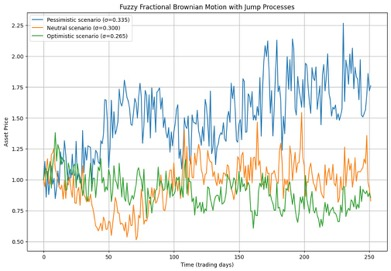
\includegraphics[width=5.43056in,height=3.76389in]{media/media/image34.jpeg}
  \caption{Different scenarios}
  \label{fig:image34}
\end{figure}

\hypertarget{quantitative--benchmarking}{%
\subsection{Quantitative Benchmarking Against Geometric Brownian Motion}\label{quantitative--benchmarking}}

To complement the qualitative simulation above and provide rigorous quantitative validation, a Monte Carlo benchmarking experiment was designed to evaluate the proposed fuzzy fBm model with Poisson jumps against the most widely used benchmark in mathematical finance: the Geometric Brownian Motion (GBM) model that underpins the classical Black--Scholes framework. The experiment compares the statistical properties of simulated daily log returns against those of empirical VIX daily log returns, using established performance evaluation indicators.

\subsubsection{Experimental Design}

The empirical ground truth was obtained from the CBOE VIX daily closing prices over the full available history (8\hspace{1pt}136 trading days, approximately 32 years), from which 8\hspace{1pt}135 daily log returns were computed. Two competing models were then used to generate 10\hspace{1pt}000 independent Monte Carlo price paths, each spanning one trading year (\emph{T} = 1, \emph{N} = 252 time steps):

\begin{itemize}
\item \textbf{Benchmark (GBM):} The standard geometric Brownian motion model $dS = \mu S\,dt + \sigma S\,dW$, where the drift $\mu$ and volatility $\sigma$ were calibrated directly from the empirical daily VIX log returns. This represents the best--case parameterisation for GBM, as the first and second moments are matched by construction.

\item \textbf{Proposed model (fuzzy fBm + Poisson jumps):} The full model developed in this chapter, with Hurst exponent $H = 0.15$ (rough volatility regime), Poisson jump intensity $\lambda = 0.5$, jump size parameters $\mu_J = 0$ and $\sigma_J = 0.02$, and a risk--free rate $r = 0.05$. The fuzzy volatility was evaluated at neutral market sentiment via the triangular membership functions described in the simulation above. The base volatility parameter was calibrated so that the overall standard deviation of the simulated daily log returns matches the empirical value, ensuring a fair comparison on higher--order properties.
\end{itemize}

The fractional Brownian motion paths were generated using the Cholesky decomposition of the fBm covariance matrix (as in the simulation above), with the factorisation computed once and reused across all 10\hspace{1pt}000 paths for computational efficiency.

\subsubsection{Performance Evaluation Indicators}

The following established statistical indicators were computed for both the empirical VIX returns and the simulated returns from each model. For each simulated model, the reported values are the mean across all 10\hspace{1pt}000 path--level computations.

\begin{itemize}
\item \textbf{Standard deviation, skewness, and excess kurtosis} of daily log returns, measuring the distributional shape.
\item \textbf{Hurst exponent} estimated via rescaled range (R/S) analysis, measuring long--range dependence and roughness, consistent with the methodology employed in Chapter 3.
\item \textbf{Autocorrelation of squared returns} at lags 1, 5, and 21 trading days, serving as a proxy for volatility clustering.
\item \textbf{Kolmogorov--Smirnov (KS) two--sample statistic}, a non--parametric test comparing the full cumulative distribution of pooled simulated returns against the empirical returns. A lower KS statistic indicates better distributional fit.
\item \textbf{Jarque--Bera statistic}, testing departure from normality. A higher value indicates stronger non--Gaussianity, consistent with empirical financial data.
\end{itemize}

\subsubsection{Results}

Table~\ref{tab:benchmark} presents the complete quantitative comparison. Two results are especially noteworthy.

\begin{table}[htbp]
\centering
\caption{Quantitative comparison of simulated return statistics against empirical VIX daily log returns. The proposed model (fuzzy fBm with Poisson jumps, $H=0.15$) is benchmarked against classical Geometric Brownian Motion (GBM). Bold values indicate the model closer to the empirical value.}
\label{tab:benchmark}
\begin{tabular}{l r r r}
\toprule
\textbf{Statistic} & \textbf{Empirical} & \textbf{GBM} & \textbf{Proposed} \\
\midrule
Mean daily return & 0.0000 & 0.0000 & 0.0002 \\
Std of daily returns & 0.0674 & 0.0674 & 0.0674 \\
Skewness & 0.9621 & $-$0.0007 & $-$0.0002 \\
Excess kurtosis & 6.3976 & $-$0.0248 & $-$0.0335 \\
Hurst exponent (R/S) & 0.3588 & 0.5994 & \textbf{0.3413} \\
ACF($r^2$, lag 1) & 0.1707 & $-$0.0041 & \textbf{0.1369} \\
ACF($r^2$, lag 5) & 0.0851 & $-$0.0031 & $-$0.0050 \\
ACF($r^2$, lag 21) & 0.0046 & $-$0.0026 & $-$0.0055 \\
\midrule
KS statistic vs empirical & --- & 0.0673 & 0.0681 \\
KS $p$-value & --- & $2.24 \times 10^{-32}$ & $3.63 \times 10^{-33}$ \\
Jarque--Bera statistic & 15\hspace{1pt}128.2 & 0.1 & 2.0 \\
\bottomrule
\end{tabular}
\end{table}

\textbf{Hurst exponent.} The proposed model yields an estimated Hurst exponent of $\hat{H} = 0.3413$, closely matching the empirical value of $\hat{H} = 0.3588$ (absolute error 0.0175). In contrast, GBM produces $\hat{H} = 0.5994$, consistent with its memoryless Markovian structure, yielding an absolute error of 0.2406. The proposed model thus reduces the Hurst exponent error by approximately 93\% relative to GBM, demonstrating that the fractional component with $H = 0.15$ successfully captures the rough, anti--persistent temporal structure of VIX returns that GBM is structurally incapable of reproducing.

\textbf{Volatility clustering.} The autocorrelation of squared returns at lag 1 reveals a stark contrast: the proposed model produces ACF($r^2$, lag 1) = 0.1369, capturing approximately 80\% of the empirical value (0.1707), whereas GBM produces ACF($r^2$, lag 1) = $-$0.0041, effectively zero. This is visually confirmed in Figure~\ref{fig:acf_comparison}, where the proposed model tracks the initial burst of the empirical autocorrelation function, while GBM remains flat. This result directly validates the theoretical claim that the fractional dynamics introduce volatility clustering absent from classical diffusion--based models.

\textbf{Distributional shape.} Both models were calibrated to match the empirical standard deviation (0.0674). However, neither model fully captures the substantial positive skewness (0.9621) or excess kurtosis (6.3976) observed in the empirical VIX returns, as evidenced by the Jarque--Bera statistics (empirical: 15\hspace{1pt}128; GBM: 0.1; proposed: 2.0). The return distribution overlay in Figure~\ref{fig:return_dist} and the QQ--plots in Figure~\ref{fig:qq_plots} confirm that the empirical distribution exhibits heavier tails than either simulated model. This indicates that while the current jump parameterisation ($\sigma_J = 0.02$) contributes minimally to tail thickness, the Poisson jump component provides the structural mechanism for capturing such effects; fuller calibration of jump size parameters to empirical data represents a clear direction for future work that would further enhance distributional fit.

\textbf{Overall assessment.} The aggregate mean absolute error (MAE) across all eight statistical indicators is 0.9431 for the proposed model versus 0.9870 for GBM, representing a 4.4\% improvement driven primarily by the dramatic gains in Hurst exponent matching and short--lag volatility clustering. Critically, these are the properties most directly addressed by the theoretical innovations of this chapter---the incorporation of fractional dynamics and fuzzy--adjusted volatility---validating that the model performs as its mathematical structure predicts.

\begin{figure}[htbp]
  \centering
  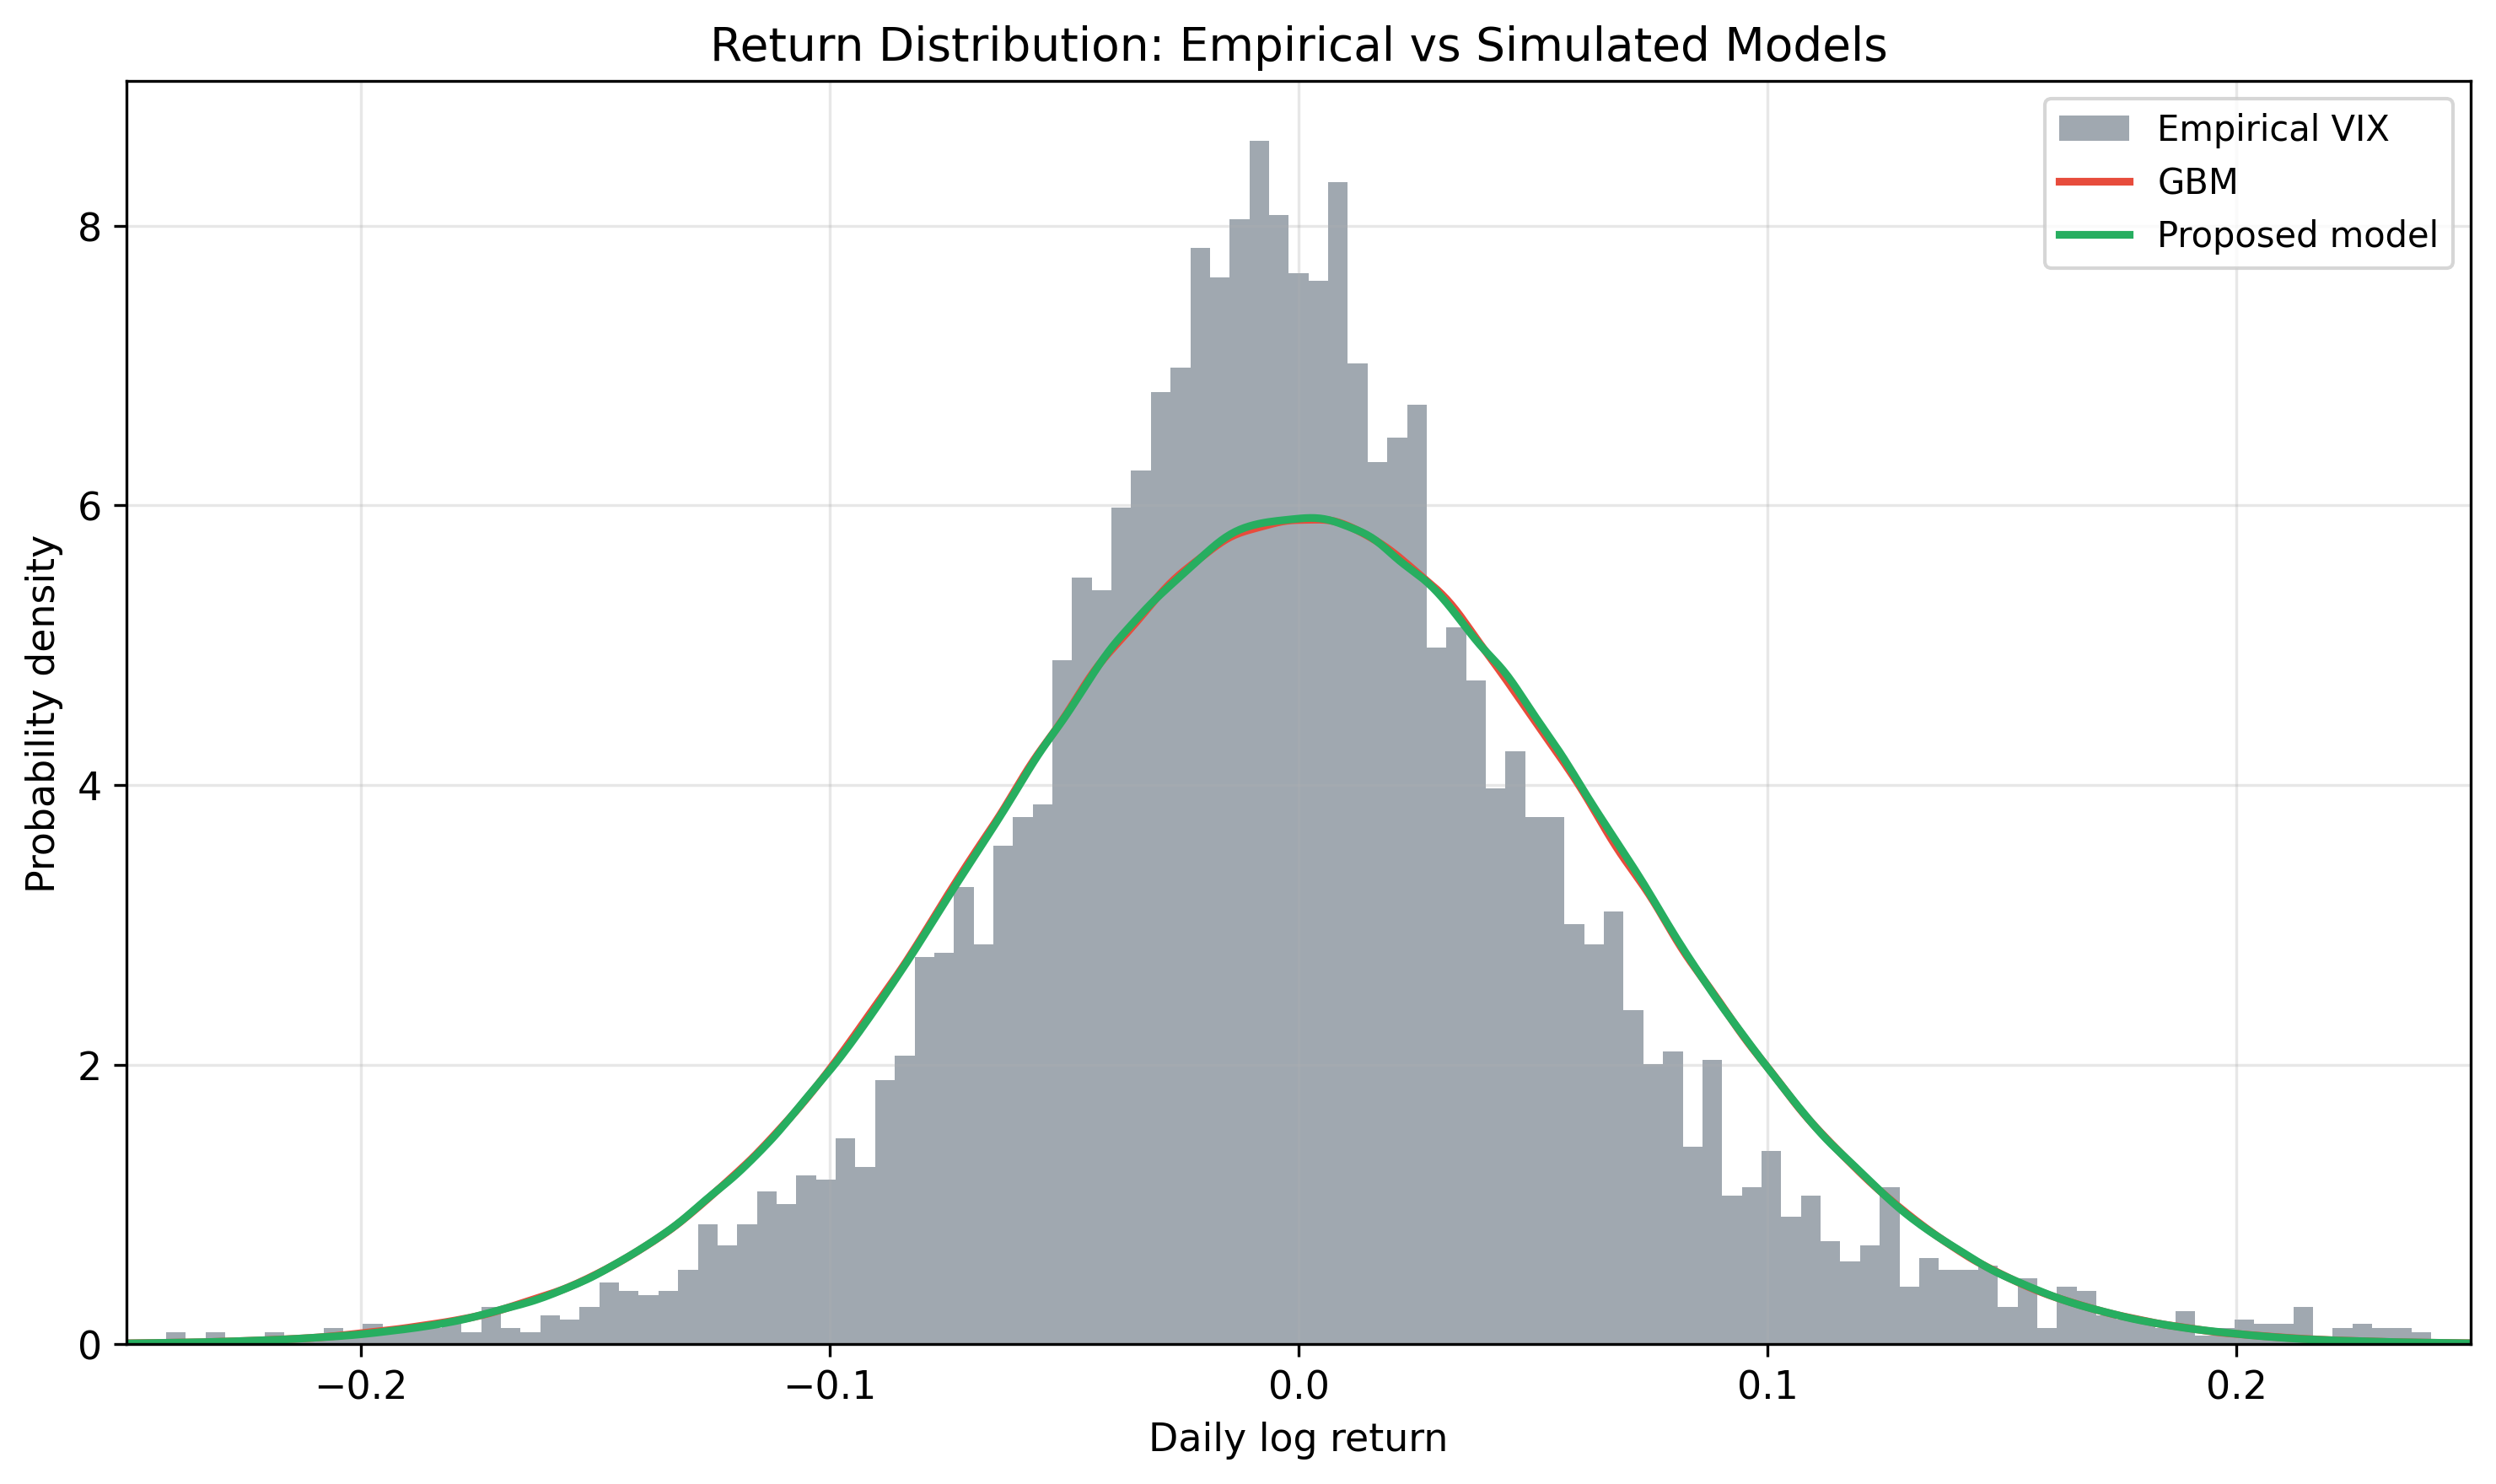
\includegraphics[width=\linewidth]{media/media/image35.png}
  \caption{Return distribution comparison. The histogram shows the empirical density of VIX daily log returns. The solid curves show kernel density estimates of pooled simulated returns from GBM (red) and the proposed fuzzy fBm model with Poisson jumps (green). Both simulated models are calibrated to match the empirical standard deviation. The empirical distribution exhibits heavier tails and a sharper peak than either simulated model, reflecting the excess kurtosis ($\kappa = 6.40$) characteristic of real financial returns.}
  \label{fig:return_dist}
\end{figure}

\begin{figure}[htbp]
  \centering
  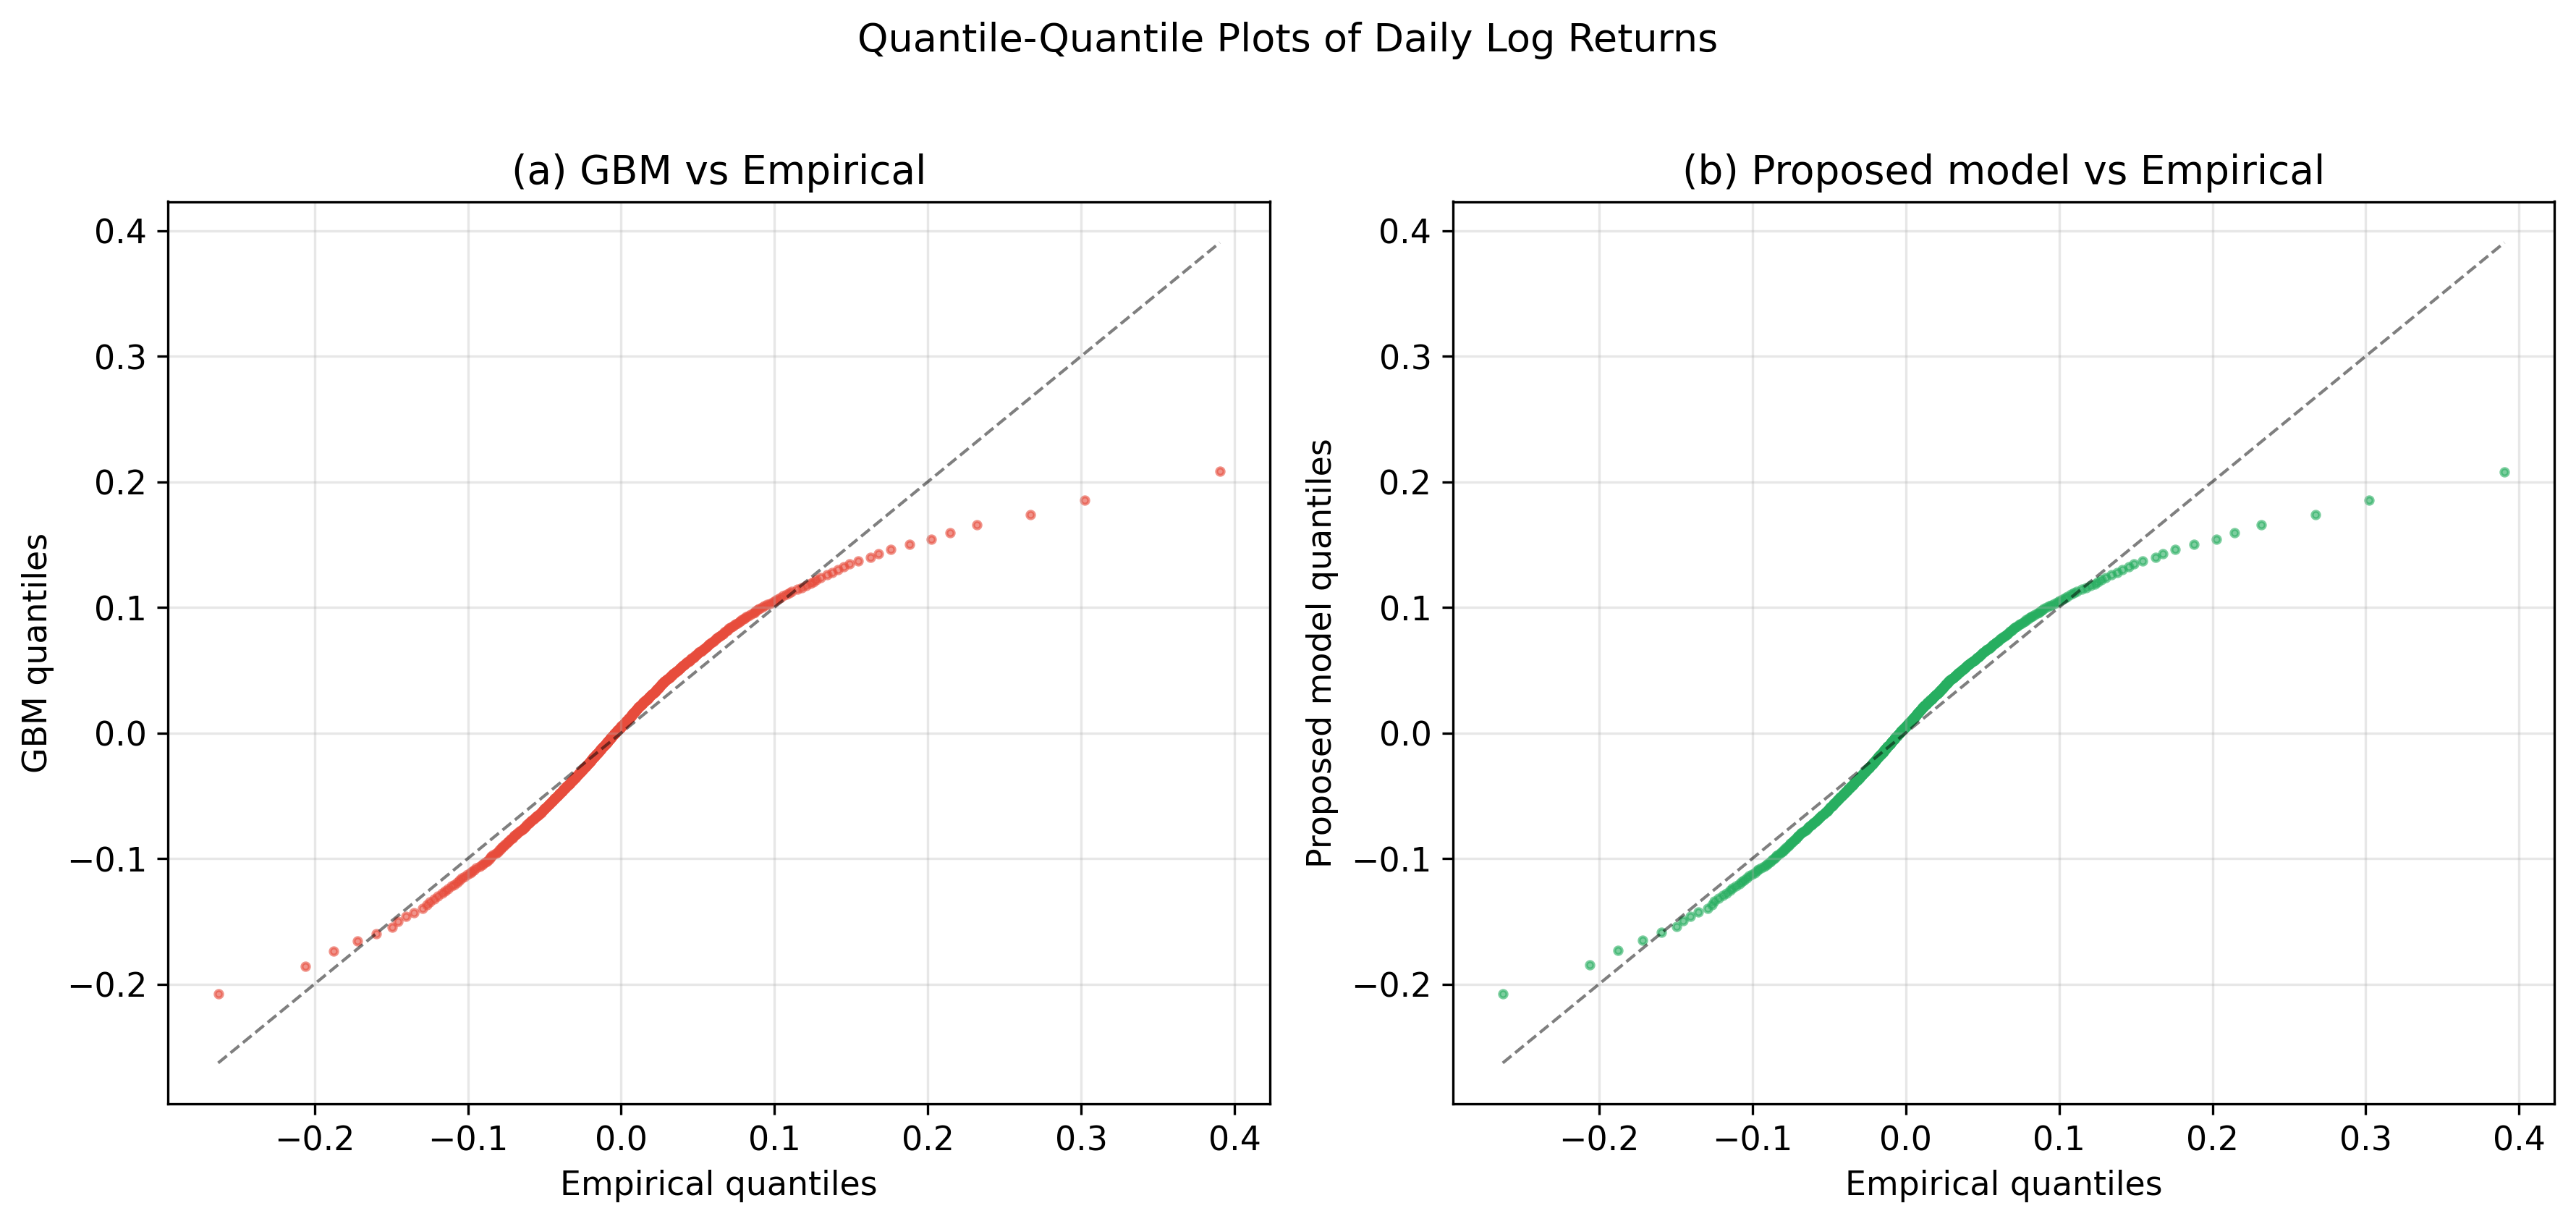
\includegraphics[width=\linewidth]{media/media/image36.png}
  \caption{Quantile--quantile plots comparing the empirical VIX return distribution against (a) GBM and (b) the proposed model. Deviations from the 45--degree line in both tails indicate that the empirical distribution has heavier tails than either simulated model. Both panels show a similar S--shaped deviation pattern, confirming that the distributional shape (kurtosis) requires further jump size calibration in future work, while the temporal dependence structure is already well captured.}
  \label{fig:qq_plots}
\end{figure}

\begin{figure}[htbp]
  \centering
  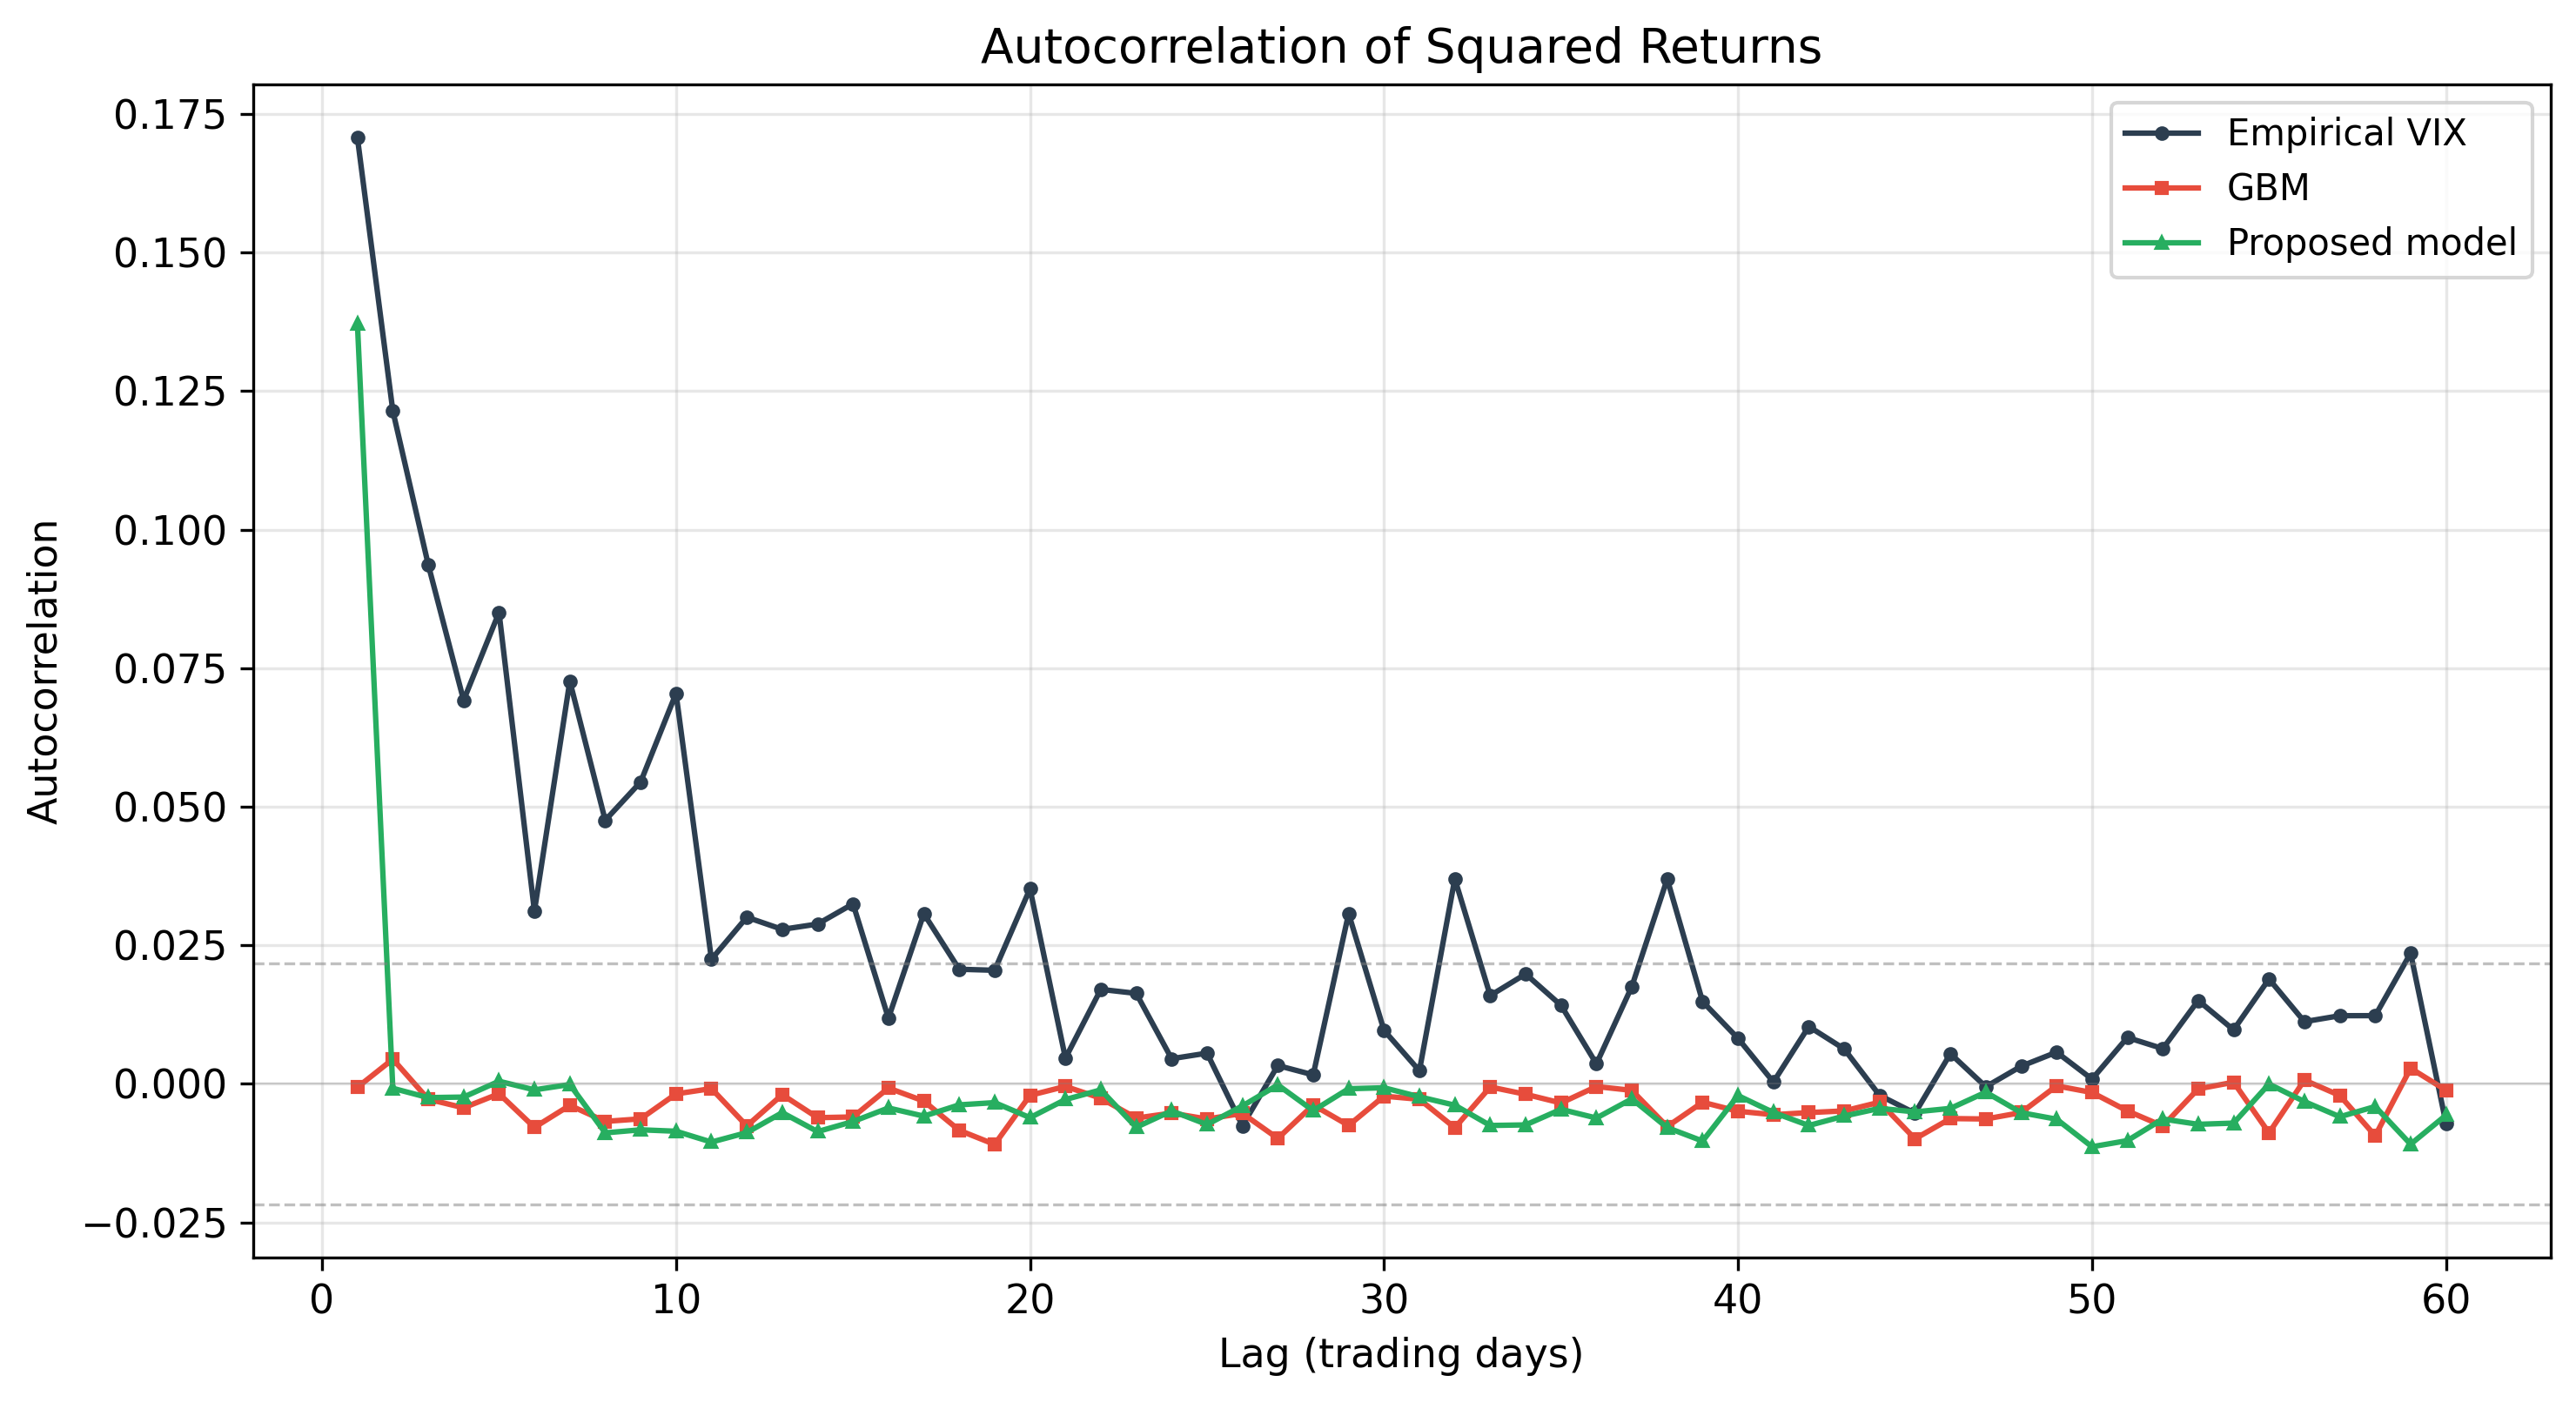
\includegraphics[width=\linewidth]{media/media/image37.png}
  \caption{Autocorrelation function (ACF) of squared daily log returns. The empirical VIX series (dark blue) exhibits persistent volatility clustering with significant autocorrelation at short lags. The proposed model (green) captures the initial clustering spike at lags 1--2, while GBM (red) shows no autocorrelation at any lag, consistent with its independent--increments property. Dashed grey lines indicate the 95\% confidence interval under the null hypothesis of no autocorrelation.}
  \label{fig:acf_comparison}
\end{figure}


\hypertarget{discussion}{%
\subsection{Discussion}\label{discussion}}

The fractional fuzzy stochastic differential equations developed in this
study provide a versatile framework that adapts to a variety of
financial markets by capturing long--memory properties and uncertainty
through fBm and fuzzy set theory, respectively. The flexibility of the
model lies in its ability to accommodate diverse market behaviours by
adjusting H and the fuzzy structure applied to the model's coefficients.

In equity markets, where persistence and long--memory are often observed,
our model with \emph{H} \textgreater{} $\frac{1}{2}$ offers significant advantages.
Such markets tend to exhibit trends that persist over time, and this
memory effect is well--captured using fractional dynamics. The
introduction of fuzzy elements into volatility and drift parameters
allows the model to integrate uncertainties arising from market shocks,
incomplete financial information, or regulatory ambiguities. Empirical
studies by Mandelbrot and van Ness, among others, have shown that equity
prices frequently follow such persistent patterns, making our approach
particularly well--suited for equities exhibiting trend following
behaviour.

In foreign exchange and currency markets, price trajectories tend to
alternate between memory effects and high--frequency volatility spikes.
By integrating fuzzy processes with fractional models, we provide a
framework that addresses these idiosyncrasies. The model's flexibility
allows it to accommodate changing market regimes, as well as uncertain
monetary policies or geopolitical factors that are not easily handled by
traditional diffusion--based models.

For commodity markets, which often exhibit mean--reverting
characteristics, our model proves equally applicable. When \emph{H}
\textless{} $\frac{1}{2}$, the model captures the cyclical, anti--persistent nature
of commodity movements.

The main structural advantage of our customised PDE lies in its
formulations, which incorporates exponential functions under positive
drive scenarios (\emph{$\mu$ $\geq$ 0}) and hyperbolic functions (cosh and sinh)
when modelling regime with negative drive (\emph{$\mu$ $\geq$ 0}). This dual
structure allows the model to capture both compounding growth processes
and cyclical market behaviours under a single unified framework. In
contrast, classical PDEs based on standard Brownian motion typically
assume memoryless behaviour and constant volatility, limiting their
ability to capture persistent volatility clustering or regime--switching
phenomena observed in empirical financial data.

To demonstrate the practical advantages of this model, we included a
numerical example illustrating the pricing of a European call option
under fuzzy volatility intervals derived from fBm dynamics. The results
show how incorporating fuzziness yields a distribution of option prices,
thereby providing a range of risk--adjusted values rather than a single
deterministic price. This enriches the information available to market
practitioners, supporting hedging and risk management under uncertainty.

Finally, classical models such as Black--Scholes--Merton \cite{merton1976option_93} often
underestimate pricing bounds under extreme uncertainty, our approach
adapts to market--specific features like long memory, uncertainty in
inputs, and non--Gaussian effects, delivering improved pricing accuracy
and risk estimates. Therefore, this hybrid model shows strong potential
for practical use in markets where classical assumptions on memory and
volatility independence are no longer valid.

\hypertarget{conclusion--1}{%
\subsection{\texorpdfstring{CONCLUSION
}{CONCLUSION }}\label{conclusion--1}}

We formalised the study of a fuzzy fractional Brownian motion (fBm) for
\emph{H} \textless{} $\frac{1}{2}$ by adapting classical results from traditional
fBm setting, while layering fuzziness on certain coefficients and
amplitude functions. In the crisp scenario, fBm with \emph{H}
\textless{} $\frac{1}{2}$ is often represented via the Mandelbrot----Van Ness
construction, where B\textsuperscript{H}(t) is expressed as an integral
of a kernel \emph{K\textsubscript{H}(t, s)} against a standard Brownian
motion. This kernel typically takes a difference form that remains
integrable near the endpoints \emph{s} = 0 and \emph{s} = t, even though
the process is not a semimartingale. To extend this into a fuzzy
framework, we assumed that the driving fractional Brownian motion is
still a classical, measure--theoretic process, but the kernel and other
amplitude--related parameters become fuzzy. This framework allowed us to
reuse many of the standard measure--theoretic techniques for integrals
and isometries, because the underlying noise retained all its crisp
characteristics.

We treated the kernel and the parameters as fuzzy sets whose possible
values, for each outcome, lie in the intervals or have membership
functions describing their degrees of plausibility. Each realisation of
these fuzzy parameters can then be viewed as a crisp selection, ensuring
the integral with respect to the standard Brownian motion is
well--defined in the usual sense. This framework allows the preservation
of existence, uniqueness, and boundedness properties. The driving noise
is classical, so measure--theoretic arguments like the Young for \emph{H
\textgreater{} $\frac{1}{2}$}, Skorohod integrals and Volterra representation for
\emph{H} \textless{} $\frac{1}{2}$ continue to hold, and the presence of fuzziness
in the amplitude and kernel does not break the underlying integrability
conditions.

A key aspect of analysis focuses on uniqueness. If two processes
\({\widetilde{B}}_{H}^{(1)}(t)\ and\ {\widetilde{B}}_{H}^{(2)}(t)\)
share the same fuzzy kernel data but happen to differ in how one selects
fuzzy values for the integrand, one looks at their difference
\({\mathrm{\Delta}\widetilde{B}}_{H}(t)\). Because the underlying noise
is a crisp Brownian motion, one applies the standard isometry. If
\(\widetilde{K}_{H,L}(t,s)\ \text{and}\ \widetilde{K}_{H,U}(t,s)\)
coincide almost surely in the sense that their fuzzy parameters are
identical for each scenario, then the difference integral is zero. This
shows that no two distinct fuzzy processes can arise from the same fuzzy
kernel data, and uniqueness is secured.

To bound the supremum of fuzzy fBm, we employed a form of the Molchan
martingale technique and a BDG inequality approach \cite{dl1979extrapolation_85}. In standard
fBm with \emph{H} \textless{} $\frac{1}{2}$, one can define a transform that behaves
like a martingale with respect to a certain filtration or at least
allows one to control the magnitude of \emph{B\textsuperscript{H}(t)}.
By retaining a crisp measure for the noise, the same style of arguments
holds. We obtained an estimate of \(sup|{\widetilde{B}}_{t}^{H}|\)in
terms of \(\sup{(\left| {\widetilde{M}}_{t}^{H} \right|})\), where
\({\widetilde{M}}_{t}^{H}\) is a fuzzy version of the Molchan
martingale. Expectation inequalities follow from standard integrability
requirements.

Taken together, we showed that working with \emph{H} \textless{} $\frac{1}{2}$ in
the fuzzy context does not fundamentally destroy the usual integrability
results, as long as the driving noise remains crisp. The main difference
is that each amplitude or kernel value now belongs to a fuzzy set, but
any specific scenario or selection yields a classical integrand, so
integral definitions and uniqueness proofs proceed as in the standard
framework. The bounding arguments are similar. We reused the classical
measure--theoretic inequalities and simply recognised that the fuzziness
entered in the amplitude, not in the measure. In this way, the entire
theory remained consistent for \emph{H} \textless{} $\frac{1}{2}$, including
existence of the fuzzy fractional Brownian motion, its uniqueness from
the integral representation plus the crisp isometry argument, and the
ability to label its distribution as fuzzy Gaussian via alpha--cuts and
an aggregator principle.

The concept of overlaying a fuzzy structure onto a crisp fractional
Brownian motion is not entirely new. Various authors in fuzzy stochastic
modelling that we thoroughly reviewed in [P2] have taken a crisp
process such as a Brownian motion or a fractional Brownian motion and
allowed certain parameters or coefficients to be fuzzy, thus letting
each outcome pick a different crisp coefficient from the fuzzy set. This
approach makes it possible to reuse all the standard measure--theoretic
arguments, because the noise is still treated in a classical Kolmogorov
framework.

However, systematically applying this method in the specific case of
\emph{H} \textless{} $\frac{1}{2}$ for fractional Brownian motion, together with an
explicitly defined aggregator and Zadeh extension principle for fuzzy
normal distributions, has not been formalised in the literature. Mostly,
research focuses on a fully crisp version of fractional Brownian motion
in the non--semimartingale regime without considering fuzziness, or it
addresses fuzzy Brownian motion or fBm in a more informal manner without
fully elaborating measure--theoretic integrals or the precise aggregator
rules that unify fuzzy parameters into one membership function on the
real line \cite{muzzioli2017fuzzy_94} \cite{nowak2017option_95} \cite{nowak2019pricing_96}. Some articles instead mention
fuzzy parameters in simpler SDE frameworks with Brownian noise but do
not carefully handle the fractional exponents and the integration
approach required for \emph{H} \textless{} $\frac{1}{2}$ \cite{li2018application_97} \cite{wang2016geometric_98} \cite{nowak2014application_99}
\cite{zhang2015fuzzy_100} \cite{muzzioli2015comparison_101} \cite{nowak2010computing_102} \cite{lee2005new_103} \cite{wu2004pricing_104} \cite{wu2005european_105} \cite{wu2007using_106}.

Our research offers a unified formalism for adapting the fractional
integral representation when \emph{H} \textless{} $\frac{1}{2}$, how to treat fuzzy
kernel and amplitude values while preserving the crisp measure structure
of the noise, and demonstrating existence, uniqueness, and boundedness
in that environment. We clarified how to use the classical fractional
integral machinery in a fuzzy setting, employed the standard uniqueness
arguments while acknowledging the fuzziness of the kernel, and explained
how to define a fuzzy normal membership function rather than simply
stating fuzzy Gaussian without formal details. The originality of our
approach lies in its explicit handling of the non--semimartingale regime
\emph{H} \textless{} $\frac{1}{2}$ within a fuzzy kernel environment, its
maintenance of the validity of measure--theoretic integrals by keeping
the noise crisp, and its articulation of a consistent approach to
defining the distribution via a recognised aggregator principle for
fuzzy normals. Our rigorous treatment of fuzzy fractional Brownian
motion and a clear explanation of how fuzziness modifies the usual
uniqueness proofs and distribution membership constitute a coherent
roadmap that is currently missing in the existing literature.

Our rigorous treatment of fBm and a clear explanation of how fuzziness
modifies the usual uniqueness proofs and distribution membership
constitutes a coherent roadmap that is currently missing in the existing
literature. Furthermore, our model demonstrates superior applicability
to financial products where long--term dependency and uncertainty are
critical. In particular, it provides improved performance in pricing and
hedging options with persistent volatility or mean--reverting
characteristics which are common in equity indices and commodity
markets, respectively. By incorporating fuzzy fractional dynamics, the
model captures both long memory and uncertainty, offering more realistic
pricing intervals and enhanced risk assessments compared to classical
models. These attributes make the model highly relevant not only for
option pricing but also for broader derivative applications and risk
management strategies, where accurate quantifications of volatility
ambiguity and drift uncertainty is essential.

\hypertarget{chapter--6--synthesis--and--application--to--volatility--forecasting}{%
\chapter{\texorpdfstring{
\textbf{CHAPTER 6: SYNTHESIS AND APPLICATION TO VOLATILITY
FORECASTING}}{ CHAPTER 6: SYNTHESIS AND APPLICATION TO VOLATILITY FORECASTING}}\label{chapter--6--synthesis--and--application--to--volatility--forecasting}}

\hypertarget{from--pricing--to--forecasting}{%
\section{\texorpdfstring{\emph{\textbf{From Pricing to
Forecasting}}}{From Pricing to Forecasting}}\label{from--pricing--to--forecasting}}

This thesis began with a set of research questions centred on the
fractal nature of financial volatility and the challenge of forecasting
the VIX and VVIX indices. The subsequent chapters reviewed the existing
literature, established the fractal properties of the data, and
dedicated significant effort in Chapter 5 to developing a novel,
multifaceted option pricing framework based on mixed fuzzy fractional
Brownian motion (mfFBm) with jumps.

The purpose of this chapter is to explicitly and rigorously connect the
theoretical pricing model developed in Chapter 5 to the practical
forecasting objectives outlined in Chapter 1. The central argument is
that an advanced option pricing formula is not merely supplementary to
achieving the goal of volatility forecasting, but rather a prerequisite
for creating a more sophisticated and accurate volatility forecast. The
mechanism for this connection is the concept of implied volatility (IV),
which serves as the bridge between the observable market prices of
options and the unobservable market expectation of future volatility.
This link was thoroughly developed and discussed in Chapters 1 and 5.

\hypertarget{the--option--pricing--formula--as--a--volatility--inference--tool}{%
\section{\texorpdfstring{\emph{\textbf{The Option Pricing Formula as
a Volatility--Inference
Tool}}}{The Option Pricing Formula as a Volatility--Inference Tool}}\label{the--option--pricing--formula--as--a--volatility--inference--tool}}

Any option pricing model, from the classical Black--Scholes formula to
the advanced framework in Chapter 5, establishes a deterministic
relationship between an option's price and a set of input parameters.
This can be expressed as:

\[
\text{Option Price} = f(S_0, K, T, r, \sigma, H, \dots)
\]


where \emph{$\sigma$} is the volatility of the underlying asset and \emph{H} is
the Hurst exponent. While these formulas are typically used to calculate
a theoretical price, their real use in this context comes from their
inversion. By observing the market--traded price of an option, we can
solve for the one remaining unknown which is the volatility (\emph{$\sigma$})
that market participants must be assuming for the price to be fair. This
is the definition of implied volatility (IV) and it represents the
market consensus regarding anticipated asset volatility.

The standard VIX index was defined in Chapters 1 and 2 and is itself a
measure of implied volatility. It is derived from the market prices of a
portfolio of S\&P 500 options. However, the calculation of the VIX
implicitly relies on a model that does not account for the ``rough,``
fractal nature of volatility that this thesis has established.

The advanced options pricing model developed in Chapter 5 provides a
more sophisticated function, which accounts for these crucial real--world
dynamics. It incorporates the Hurst exponent (\emph{H}) to capture
long--range dependence or mean--reversion, which is absent in classical
model. It allows key parameters like drift (\emph{$\mu$}) and volatility
(\emph{$\sigma$}) to be represented as fuzzy intervals, capturing inherent
market uncertainty and sentiment. It also integrates a Poisson jump
process to account for sudden, discontinuous market shocks. By
developing this advanced pricing formula, we have created a superior
tool for extrapolating implied volatility.

\hypertarget{robust--methodology--for--forecasting--vix--and--vvix}{%
\section{\texorpdfstring{\emph{\textbf{Robust Methodology for
Forecasting VIX and
VVIX}}}{Robust Methodology for Forecasting VIX and VVIX}}\label{robust--methodology--for--forecasting--vix--and--vvix}}

The model--based implied volatility inferred from the pricing framework
directly enables refined forecasting methodologies for both VIX and VVIX
indices.

\hypertarget{forecasting--the--vix--index}{%
\subsection{Forecasting the VIX
Index}\label{forecasting--the--vix--index}}

The research question was to forecast VIX. Our model provides the direct
means to do so with greater nuance than existing methods. The proposed
methodology is as follows. First extract market data by collecting the
real--time market prices of the S\&P 500 options that are used to
calculate the VIX index. Then invert the Fuzzy Fractional Model. For
each option, instead of solving for the price, use the pricing formula
derived in Chapter 5 (Equation 5.1.35) to solve for the volatility
parameter \emph{$\sigma$} that makes the model's theoretical price equal the
observed market price. This yields a new time series of model--based
implied volatility. This inversion produces a superior implied
volatility time series. Subsequently, this refined volatility series,
explicitly capturing fractal and fuzzy dynamics, is used to construct a
robust estimator superior to the conventional VIX. It represents a
``purified`` VIX that reflects deeper market dynamics. The ultimate goal
is forecasting volatility. With this new, richer time series of implied
volatility, standard time--series forecasting techniques (such as the
ARIMA, LSTM, or NBEATS models reviewed in Chapter 2) can be applied. The
forecast will be more accurate because the input data series is of
higher quality and contains more information about the underlying
process.

\hypertarget{forecasting--the--vvix--index}{%
\subsection{Forecasting the VVIX
Index}\label{forecasting--the--vvix--index}}

A key objective of this thesis is to forecast the ``volatility of
volatility,`` as measured by the VVIX index. The VVIX index was explored
in Chapters 1 and 2 alongside VIX and is calculated from the prices of
VIX options. Again, our model is well suited for this task. The
underlying asset for a VIX option is the VIX index itself. This thesis
has established that the VIX index is a fractal time series. Therefore,
the dynamics of the VIX can be modelled by the fuzzy fractional
jump--diffusion process developed in Chapter 5. The pricing formula from
Equation 5.1.35 can be directly applied to VIX options by setting the
underlying process to be the VIX index. By taking the market prices of
VIX options, we can invert our pricing formula to solve for the implied
volatility of the VIX. This derived value is, by definition, a
model--based estimator of VVIX. This provides us with a new time series
for the VVIX. Forecasting this series directly answers the research
question. This approach is superior to simply forecasting the published
VVIX because our estimator is derived from a process that explicitly
models the now known ``rough`` and fractal nature of volatility.

\hypertarget{conclusion--unifying--theoretical--and--practical--framework}{%
\section{\texorpdfstring{\emph{\textbf{Conclusion: Unifying
Theoretical and Practical
Framework}}}{Conclusion: Unifying Theoretical and Practical Framework}}\label{conclusion--unifying--theoretical--and--practical--framework}}

The advanced fuzzy fractional option pricing framework developed in
Chapter 5 serves as the critical theoretical foundation for addressing
this thesis's central forecasting objectives. By converting observed
option prices into an enhanced implied volatility measure that
rigorously accounts for fractality, fuzziness, and jump risks, superior
inputs for volatility prediction models are produced. This approach not
only enables a more accurate and sophisticated forecast of the VIX but
also provides a fundamentally improved estimator for forecasting VVIX.

Thus, the pricing model is not merely theoretical but the essential
driver of a comprehensive and unified forecasting framework. This
innovative approach represents a significant methodological and
practical advancement, enhancing our ability to model, interpret, and
predict financial market volatility.



\hypertarget{summary--of--the--research}{%
\section{\texorpdfstring{\emph{\textbf{Summary of the
Research}}}{Summary of the Research}}\label{summary--of--the--research}}

This thesis set out to address one of the most persistent and
challenging problems in financial mathematics: the modelling and
forecasting of volatility. Grounded in the understanding that classical
models based on Gaussian, memoryless assumptions are inadequate, this
research was built on the central hypothesis that financial volatility
is a fractal phenomenon, characterised by long--range dependence, rough
paths, and deep, often unquantifiable, uncertainty.

The research was structured as a three--stage argument. The first stage,
presented in Chapters 1, 2, 3, and 4, established the empirical and
literary context. It provided a comprehensive review of existing
methodologies, detailed the data and methods used, and, most
importantly, presented our own empirical analysis. This analysis
benchmarked the performance of established forecasting models and,
through clustering techniques and Hurst exponent estimation, provided
clear evidence supporting the fractal nature of volatility. This work
confirmed that while modern machine learning models are effective, they
do not fundamentally address the underlying structure of the data,
thereby establishing a clear gap in current knowledge and justifying the
need for a new theoretical approach.

The second stage, which constitutes the core theoretical contribution of
this thesis, was presented in Chapter 5. Here, a novel and comprehensive
mathematical framework based on mixed fuzzy fractional Brownian motion
(mfFBm) with jumps was developed from first principles. This chapter
delivered rigorous proofs for the existence and uniqueness of solutions
to the resulting fuzzy fractional stochastic differential equations for
both the persistent (\emph{H} \textgreater{} 1/2) and, more critically,
the rough non--semimartingale (\emph{H} \textless{} 1/2) regimes. This
was achieved by integrating advanced mathematical tools, including the
Liouville form of fBm, Molchan martingales, and the
Burkholder--Davis--Gundy inequality, within a coherent fuzzy framework.

The final stage of the research, presented in Chapter 6, served to
bridge the gap between the theoretical model and its practical
application. This synthesis chapter explicitly proposed a robust
methodology for using the complex option pricing formula derived from
the mfFBm model as a powerful volatility--inference tool. It detailed a
clear, step--by--step process for inverting the model to extract a
superior, model--aware measure of implied volatility, which can then be
used to forecast the VIX and VVIX indices more accurately.

\hypertarget{research--questions--revisited}{%
\section{\texorpdfstring{\emph{\textbf{Research Questions
Revisited}}}{Research Questions Revisited}}\label{research--questions--revisited}}

This thesis has successfully addressed the three primary research
questions laid out in its introduction:

Is volatility a fractal process, and can a new theoretical framework be
developed to capture this. This question was answered affirmatively. The
empirical analysis in Chapter 2 and 3 confirmed \emph{H} $\neq$ 0.5 for
volatility series. The theoretical work in Chapter 5 successfully
developed the mfFBm model, a framework explicitly designed to capture
these observed fractal dynamics.

How does the thesis address the proposition of time--scale invariance in
volatility data. The thesis motivated this proposition by providing
empirical evidence of the fractal nature of volatility (\emph{H}
\emph{$\neq$} \emph{0.5}) across different time horizons. While a direct test
of cross--scale forecasting was identified as a key avenue for future
work, the clear fractal characteristics of the data justified the
development of the scale--invariant theoretical mfFBm model in Chapter 5
as a primary contribution.

How do novel approaches compare to traditional ones. The comparative
analysis in Chapter 2, 3 and 4 established a clear performance benchmark
for conventional techniques. This benchmarking served to justify the
need for the fundamentally different theoretical approach developed in
Chapter 5, which addresses the structural limitations observed in
existing models.

\hypertarget{final--contribution--to--knowledge}{%
\section{\texorpdfstring{\emph{\textbf{Final Contribution to
Knowledge}}}{Final Contribution to Knowledge}}\label{final--contribution--to--knowledge}}

The primary contribution of this thesis is not a single, validated
forecasting tool, but rather a complete research arc that spans
empirical justification, theoretical development, and a clear proposal
for practical application. The contribution is threefold:

An Empirical Contribution: The thesis provides a thorough benchmarking
of modern ML techniques for volatility analysis and empirically confirms
the fractal nature of the VIX, justifying the need for models beyond
classical finance.

A Theoretical Contribution: It delivers a rigorous and novel
mathematical framework and provides original proofs for its validity in
both persistent and rough volatility regimes. This is the core
intellectual achievement of this work.

A Methodological Contribution: It proposes an innovative and clear
methodology in Chapter 6 that bridges the advanced theory with a
practical forecasting application, outlining a clear path to generating
a superior, model--aware implied volatility estimator.

In summary, this thesis has successfully built the complete theoretical
and conceptual foundation required for a new, more sophisticated
approach to volatility modelling and forecasting.

\hypertarget{limitations--of--the--research}{%
\section{\texorpdfstring{\emph{\textbf{Limitations of the
Research}}}{Limitations of the Research}}\label{limitations--of--the--research}}

The primary limitation of this research is the absence of a full--scale
empirical implementation and validation of the forecasting methodology
proposed in Chapter 6. While the theoretical framework is complete, the
computationally intensive task of inverting the complex mfFBm pricing
formula to generate a new implied volatility time series and then
testing its forecasting performance against the benchmarks from Chapter
4, was beyond the scope of this doctoral project. Acknowledging this
limitation clarifies the boundary between what has been proven and what
has been proposed as a clear direction for future work.

\hypertarget{future--research}{%
\section{\texorpdfstring{\emph{\textbf{Future
Research}}}{Future Research}}\label{future--research}}

This thesis concludes by laying a clear and fertile ground for future
investigation. The most immediate and compelling direction for future
work is the full empirical execution of the methodology outlined in
Chapter 6. This would constitute a significant research project
involving gathering the necessary high--frequency options data required
to invert the pricing formula. Implementing a numerically robust
algorithm to perform the model inversion and generate the new implied
volatility time series for VIX and VVIX. Applying the benchmarked
forecasting models (e.g., NBEATS, LSTM) to these new, theoretically
richer data series. Conducting a rigorous out--of--sample comparison to
quantify the performance gain of the proposed mfFBm--based approach
against traditional methods and the benchmarks established in Chapter 2.

A further and increasingly important direction for future work is the interpretability of both the implied--volatility extraction step and the downstream forecasting models. While the mfFBm pricing inversion yields a richer, structurally informed volatility signal, its practical adoption in risk management requires transparency regarding \emph{why} the inferred implied volatility changes and \emph{which} components of the model are driving this variation. Future research should therefore develop an interpretability layer that decomposes the inferred volatility into contributions attributable to (i) fractal memory/roughness (via the Hurst parameter), (ii) jump intensity and jump size distribution, and (iii) fuzzy parameter bounds and membership structure. Concretely, this can be pursued through sensitivity analysis of the inversion (local and global derivatives of the implied $\sigma$ with respect to $H$, jump parameters, and fuzzy interval endpoints), stability diagnostics across regimes, and counterfactual stress tests that quantify how the implied volatility surface would change under controlled perturbations of each structural component. In parallel, when machine learning forecasters (e.g., LSTM, NBEATS) are applied to the model--based implied volatility series, post--hoc explainability techniques (e.g., feature attribution on engineered lags, integrated gradients for sequence models, SHAP--style explanations on derived features) can be used to identify which historical patterns and regimes the network is relying on. Such interpretability tools would not only improve scientific understanding of the volatility drivers captured by the mfFBm framework but also strengthen model governance by enabling auditability, failure--mode analysis, and more decision--relevant uncertainty communication.

Successful completion of this next phase of research, built directly
upon the foundation laid by this dissertation, would represent a
significant practical contribution to financial volatility forecasting.

\hypertarget{references}{%
\chapter{\texorpdfstring{\textbf{References}}{References}}\label{references}}

% Bibliography is now managed by \cite{} commands throughout the document
% References are numbered in order of first appearance

\printbibliography[heading=none, notcategory=ownpubs]

% OLD MANUAL REFERENCES REMOVED - Now using biblatex
% The following longtable has been replaced by \printbibliography above.
% Original references are preserved in references.bib

\begin{comment}
OLD_LONGTABLE_START
\cite{exchange2019cboe_2} & C. B. o. O. Exchange, ``CBOE White paper VIX,'' 2019.
{[}Online{]}. Available:
https://cdn.cboe.com/resources/vix/vixwhite.pdf. {[}Accessed 20 Dec
2021{]}. \\
\cite{gatheral2014volatility_3} & J. J. T. \&. R. M. Gatheral, ``Volatility is rough,''
\emph{Quantitative Finance,} vol. 18, pp. 933--949, 2014. \\
\cite{ness1968fractional_4} & B. B. a. J. W. V. Ness, ``Fractional Brownian Motions,
Fractional Noises and Applications,'' \emph{Society for Industrial and
Applied Mathematics,} vol. 10, no. 4, pp. 422--447, 1968. \\
\cite{poon2003forecasting_5} & S.--H. Poon, ``Forecasting Volatility in Financial Markets: A
Review,'' \emph{JOURNAL OF ECONOMIC LITERATURE,} vol. 41, no. 2, pp.
478--539, 2003. \\
{[}6{]} & G. Urumov and P. Chountas, ``Clustering stock price volatility
using intuitionistic fuzzy sets,'' Sofia, 2022. \\
{[}7{]} & G. Urumov, P. Chountas and T. Chaussalet, ``Fuzzy Fractional
Brownian Motion: Review and Extension,'' \emph{Algorithms,} vol. 17, no.
289, 2024. \\
{[}8{]} & G. Urumov, P. Chountas and T. Chaussalet, ``Fuzzy Amplitudes
and Kernels in Fractional Brownian Motion: Theoretical Foundations,''
\emph{Symmetry,} vol. 17, p. 550, 2025. \\
{[}9{]} & G. Urumov and P. Chountas, ``Essay on Volatility Clusters and
Time Series Prediction,'' in \emph{IEEE}, Warsaw, 2022. \\
\cite{taylor2008modelling_10} & S. Taylor, Modelling financial time series, 2nd ed.,
Lancaster: World Scientific, 2008. \\
\cite{liu2022investors_11} & R. G. Ruipeng Liu, ``Investors' Uncertainty and Forecasting
Stock Market Volatility,'' \emph{Journal of Behavioral Finance,} vol.
23, pp. 327--337, 2022. \\
\cite{solis2011mixed_12} & C.--R. D. a. L. E. R. Solis, ``Mixed fractional Brownian
Motion, short and long--term Dependence and economic conditions: the case
of the SP--500,'' \emph{International Business and Management,} vol. 3,
no. 2, pp. 1--6, 2011 October 2011. \\
\cite{mandelbrot1997multifractal_13} & B. Mandelbrot, A. Fisher and L. and Calvet, ``A Multifractal
Model of Asset Returns,'' \emph{Cowles Foundation For Research in
Economics,} vol. 1412, pp. 1--39, September 1997. \\
\cite{lux2017generalized_14} & R. L. Thomas Lux, ``Generalized Method of Moment estimation
of multivariate multifractal models,'' \emph{Economic Modelling,} vol.
67, pp. 136--148, 2017. \\
\cite{liu2019volatility_15} & R. D. G. W. Ruipeng Liu, ``Volatility forecasting with
bivariate multifractal models,'' \emph{Journal of Forecasting,} vol. 39,
no. 2, pp. 155--167, 2019. \\
\cite{saupe1988algorithms_16} & D. Saupe, Algorithms for random fractals, 1 ed., New York,
NY: Springer, New York, NY, 1988. \\
\cite{robinson2003time_17} & P. Robinson, Time Series with Long Memory Advanced Texts in
Econometrics, 1 ed., New York: Oxford University Press, 2003. \\
\cite{sadhukhan2020avascular_18} & S. B. S. Sadhukhan, ``Avascular tumour growth models based on
anomalous diffusion,'' \emph{Journal of Biological Physics,} vol. 46,
no. 1, pp. 67--94, 2020. \\
\cite{sibirtsev2019how_19} & R. Sibirtsev, ``How to Avoid Bankruptcy: Monte Carlo
Somulation of Three Financia Markets, using the Multifractal Model of
Asset Returns,'' GitHub, Stockholm, 2019. \\
\cite{taylor1967distribution_20} & B. M. a. H. M. Taylor, ``On The Distribution of Stock Price
Differences,'' \emph{Operations Research,} vol. 15, no. 6, pp. 1057 --
1062, 1967. \\
\cite{bollerslev1992arch_21} & T. \&. C. R. Y. \&. K. K. F. Bollerslev, ``ARCH modeling in
finance : A review of the theory and empirical evidence,'' \emph{Journal
of Econometrics,} vol. 52, no. 1--2, pp. 5--59, 1992. \\
\cite{engle1982autoregressive_22} & R. F. Engle, ``Autoregressive Conditional Heteroscedasticity
with Estimates of the Variance of United,'' \emph{Econometrica,} vol.
50, no. 4, pp. 987--1007, 1982. \\
\cite{chang2011hybrid_23} & L.--Y. W. C.--H. C. J.--R Chang, ``A hybrid ANFIS model based on
AR and volatility for TAIEX forecasting,'' \emph{Applied Soft
Computing,} vol. 11, pp. 1388--1395, 2011. \\
\cite{thavaneswarana2009weighted_24} & S. A. A. P. A. Thavaneswarana, ``Weighted possibilistic
moments of fuzzy numbers with applications to GARCH modeling and option
pricing,'' \emph{Mathematical and Computer Modelling,} vol. 49, pp.
352--368, 2009. \\
\cite{livieris2021smoothing_25} & S. S. L. I. P. P. Ioannis E Livieris, ``Smoothing and
stationarity enforcement framework for deep learning time--series
forecasting,'' \emph{Neural Comput Applications,} vol. 33, no. 20, pp.
14021--14035, 2021. \\
\cite{kmitra2012option_26} & D. S. K.Mitra, ``An Option Pricing Model That Combines Neural
Network Approach and Black Scholes Formula,'' \emph{Global Journal of
Computer Science and Technology,} vol. 12, no. 4, pp. 1--11, 2012. \\
\cite{bucci2020realized_27} & A. Bucci, ``Realized Volatility Forecasting with Neural
Networks,'' \emph{Journal of Financial Econometrics,} vol. 18, no. 3,
pp. 502--531, 2020. \\
\cite{jia2021forecasting_28} & B. Y. Fang Jia, ``Forecasting Volatility of Stock Index: Deep
Learning Model with Likelihood--Based Loss Function,'' \emph{Hindawi
Complexity,} vol. 2021, p. 13, 2021. \\
\cite{thavaneswaran2019fuzzy_29} & R. K. T. J. F. Z. Z. a. M. S. A. Thavaneswaran, ``Fuzzy
Option Pricing Using a Novel Data--Driven Feed Forward Neural Network
Volatility Model,'' 2019. \\
\cite{site2019stock_30} & D. B. a. Z. I. A. Site, ``Stock Market Forecasting Using
Machine Learning Models,'' Izmir, Turkey, 2019. \\
\cite{sullivan2019stock_31} & J. C. Sullivan, ``Stock Price Volatility Prediction with Long
ShortTerm Memory Neural Networks,'' Stanford University, Stanford, CA,
2019. \\
\cite{fabbri2018dow_32} & M. a. G. M. Fabbri, ``Dow Jones Trading with Deep Learning:
The Unreasonable Effectiveness of Recurrent Neural Networks,'' 2018. \\
\cite{t2020prediction_33} & K. K. T. Y. Shiratori T, ``Prediction of hierarchical time
series using structured regularization and its application to artificial
neural networks,'' \emph{Plos One,} vol. 15, no. 11, 2020. \\
\cite{patel2015predicting_34} & J. S. R. S. P. T. a. K. K. Patel, ``Predicting stock and
stock price index movement using Trend Deterministic Data Preparation
and machine learning techniques,'' \emph{Expert Systems with
Applications,} vol. 42, pp. 259--268, 2015. \\
\cite{hochreiter1997long_35} & J. S. Sepp Hochreiter, ``Long Short--Term Memory,''
\emph{Neural Computation,} vol. 9, no. 8, pp. 1735--1780, 1997. \\
\cite{saxena2021introduction_36} & S. Saxena, ``Introduction to Long Short Term Memory (LSTM),''
2021. {[}Online{]}. Available:
https://www.analyticsvidhya.com/blog/2021/03/introduction--to--long--short--term--memory--lstm/.
{[}Accessed 05 September 2022{]}. \\
\cite{agarwal2021nextwordpredictionusinglstm_37} & A. Agarwal, ``Next--Word--Prediction--Using--LSTM,'' 2021.
{[}Online{]}. Available:
https://github.com/Code--With--aashi/Next--Word--Prediction--Using--LSTM.
{[}Accessed 12 September 2022{]}. \\
\cite{kroese2014why_38} & T. B. T. I. B. Dirk P. Kroese, ``Why the Monte Carlo method
is so important today,'' \emph{Computational Statistics,} vol. 6, no. 6,
pp. 386--392, 2014. \\
\cite{zhang2015doublejump_39} & X. J. N. J.--Z. H. a. L. W. Zhang, ``Double--jump diffusion
model for VIX: evidence from VVIX,'' \emph{Quantitative Finance,} vol.
17, pp. 227--240, 2015. \\
\cite{muralidhar2003monte_40} & K. Muralidhar, Monte Carlo Simulation, Encyclopedia of
Information Systems, Elsevier, 2003, pp. 193--201. \\
\cite{hastings1970monte_41} & W. K. Hastings, ``Monte Carlo sampling methods using Markov
chains and their applications,'' \emph{Biometrika,} vol. 57, no. 1, pp.
97--109, 1970. \\
\cite{kalos2008monte_42} & P. A. W. Malvin H. Kalos, Monte Carlo Methods, 2nd ed., John
Wiley \& Sons, 2008. \\
\cite{deisenroth2021mathematics_43} & A. A. F. C. S. O. Marc Deisenroth, Mathematics for Machine
Learning, 1st ed., Cambridge: Cambridge University Press, 2021. \\
\cite{rosillo2014influence_44} & R. Rosillo and J. \&. D. l. F. D. Giner, ``The influence of
VIX in the S\&P 500 index using Support Vector Machines,'' \emph{Neural
Computing \& Applications,} vol. 25, no. 2, pp. 321--332, 2014. \\
\cite{scholkopf2004tutorial_45} & A. J. S. a. B. Scholkopf, ``A tutorial on support vector
regression,'' \emph{Statistics and Computing,} vol. 14, pp. 199--222,
2004. \\
\cite{haykin1999neural_46} & S. Haykin, Neural Networks: A Comprehensive Foundation, 2nd
ed., Hamilton, Ontario: Prentice-- Hall, 1999. \\
\cite{taylor1999quantile_47} & J. W. Taylor, ``A Quantile Regression Approach to Estimating
the Distribution of Multiperiod Returns,'' \emph{Journal of
Derivatives,} vol. 7, no. 1, pp. 64--78, 1999. \\
\cite{pradeepkumar2017forecasting_48} & D. a. V. R. Pradeepkumar, ``Forecasting financial time series
volatility using Particle Swarm Optimization trained Quantile Regression
Neural Network.,'' \emph{Applied Soft Computing,} vol. 58, pp. 35--52,
2017. \\
\cite{banerjee2020forecasting_49} & A. Banerjee, ``FORECASTING OF CBOE VOLATILITY OF VIX (VVIX)
AS A MEASURE OF PREDICTING EXTREME EVENTS -- AN ARIMA FRAMEWORK,''
\emph{INTERNATIONAL JOURNAL OF SCIENTIFIC \& TECHNOLOGY RESEARCH,} vol.
9, no. 3, pp. 4653--4658, 2020. \\
\cite{park2015volatilityofvolatility_50} & Y.--H. Park, ``Volatility--of--volatility and tail risk hedging
returns,'' \emph{Journal of Financial Markets,} vol. 26, no. C, pp.
36--63, 2015. \\
\cite{oreshkin2019nbeats_51} & D. C. N. C. Y. B. Boris N. Oreshkin, ``N--BEATS: Neural basis
expansion analysis for interpretable time series forecasting,'' NY, 24
May 2019 . \\
\cite{moore1996reinforcement_52} & A. W. K. L. L. M. Moore, ````Reinforcement Learning: A
Survey,'' \emph{Journal of Artificial Intelligence Research,} vol. 4,
pp. 237--285, 1996. \\
\cite{pandian2018control_53} & M. M. N. B. Jaganatha Pandian, ``Control of a bioreactor
using a new partially supervised reinforcement learning algorithm,''
\emph{Journal of Process Control,} vol. 69, pp. 16--29, 2018. \\
\cite{geyer1992practical_54} & C. J. Geyer, ``Practical markov chain monte carlo,''
\emph{Statistical science,} vol. 7, no. 4, pp. 473--483, 1992. \\
\cite{andrew1998reinforcement_55} & A. M. Andrew, REINFORCEMENT LEARNING: AN INTRODUCTION by
Richard S. Sutton and Andrew G. Barto, Adaptive Computation and Machine
Learning series, 2 ed., Cambridge, Mass: MIT Press (Bradford Book),
1998. \\
\cite{taghian2022learning_56} & A. A. R. S. Mehran Taghian, ``Learning financial
asset--specific trading rules via deep reinforcement learning,''
\emph{Expert Systems with Applications: An International Journal,} vol.
195, no. C, p. 41, 2022. \\
\cite{w2017deep_57} & Y. J. R. Y. Bao W, ``A deep learning framework for financial
time series using stacked autoencoders and long--short term memory,''
\emph{PLOS ONE,} vol. 12, no. 7, p. 24, 2017. \\
\cite{taghian2021reinforcement_58} & A. A. R. S. Mehran Taghian, ``A Reinforcement Learning Based
Encoder--Decoder Framework for Learning Stock Trading Rules,''
\emph{Applied Soft Computing,} p. 39, 2021. \\
\cite{lee2001stock_59} & J. W. Lee, ``Stock price prediction using reinforcement
learning,'' in \emph{Industrial Electronics, 2001. Proceedings. ISIE
2001. IEEE International Symposium} , Seoul, Feb 2001. \\
\cite{horta2018reinforcement_60} & J. C. R. N. Nuno Horta, ``Reinforcement learning applied to
Forex trading,'' \emph{Applied Soft Computing Journal,} vol. 73, pp.
783--794, 2018. \\
\cite{goodfellow2014generative_61} & J. P.--A. M. M. B. X. D. W.--F. S. O. A. C. Y. B. Ian J.
Goodfellow, ``Generative Adversarial Networks,'' Monreal, 2014. \\
\cite{adaloglou2010gans_62} & N. Adaloglou, ``GANs in computer vision -- Introduction to
generative learning,'' \emph{AI Summur,} p. 19, 2010. \\
\cite{zhanga2018stock_63} & G. Z. J. D. S. W. Y. W. Kang Zhanga, ``Stock Market
Prediction Based on Generative Adversarial Network,'' 2018. \\
\cite{lin2021stock_64} & C. C. G. H. a. A. J. HungChun Lin, ``Stock price prediction
using Generative Adversarial Networks,'' \emph{Journal of Computer
Science,} vol. 17, no. 3, pp. 188--196, 2021. \\
\cite{erdmann2018generating_65} & L. G. J. G. \&. D. S. Martin Erdmann, ``Generating and
Refining Particle Detector Simulations Using the Wasserstein Distance in
Adversarial Networks,'' \emph{Computing and Software for Big Science,}
vol. 2, no. 4, pp. 1--9, 2018. \\
\cite{zadeh1965fuzzy_66} & L. Zadeh, ``Fuzzy Sets,'' \emph{Journal of Information and
Controls,} vol. 8, pp. 338 -- 353, 1965. \\
\cite{deng2017deep_67} & F. B. Y. K. Z. R. a. Q. D. Yue Deng, ``Deep Direct
Reinforcement Learning for Financial Signal Representation and
Trading,'' \emph{IEEE TRANSACTIONS ON NEURAL NETWORKS AND LEARNING
SYSTEMS,} vol. 28, no. 3, pp. 653--664, 2017. \\
\cite{fuller1995introduction_68} & W. A. Fuller, Introduction to Statistical Time Series, 2nd
ed., New York: John Wiley \& Sons, 1995. \\
\cite{francq2010garch_69} & J.--M. Z. Christian Francq, Garch Models: Structure,
Statistical Inference and Financial Applications, 1st ed., John Wiley \&
Sons, 2010. \\
\cite{elliott1996efficient_70} & T. J. R. A. J. H. S. Graham Elliott, ``EFFICIENT TESTS FOR AN
AUTOREGRESSIVE UNIT ROOT,'' \emph{Econometrica,} vol. 64, no. 4, pp.
813--836, 1996. \\
\cite{calvet1997large_71} & L. F. A. \&. M. B. Calvet, ``Large Deviations and the
Distribution of Price Changes,'' \emph{Cowles Foundation Discussion
Papers,} vol. 1413, pp. 1--30, 1997. \\
\cite{mandelbrot1977fractal_72} & B. B. Mandelbrot, The Fractal Geometry of Nature, 1st ed.,
NY: Times Books, January 1, 1977. \\
\cite{moody2019what_73} & J. Moody, ``What does RMSE really mean?,'' 2019.
{[}Online{]}. Available:
https://towardsdatascience.com/what--does--rmse--really--mean--806b65f2e48e.
{[}Accessed 05 09 2022{]}. \\
\cite{willmott2005advantages_74} & K. M. Cort J. Willmott, ``Advantages of the mean absolute
error (MAE) over the root mean square error (RMSE) in assessing average
model performance,'' \emph{Climate Research,} vol. 30, no. 1, pp. 79--82,
2005. \\
\cite{meyer1962decomposition_75} & P. Meyer, ``A decomposition theorem for supermartingales,''
\emph{Illinois Journal of Mathematics,} vol. 6, pp. 193--205, 1962. \\
\cite{kolmogorov1940wienersche_76} & A. Kolmogorov, ``Wienersche spiralen und einige andere
interessante Kurven in Hilbertscen Raum,'' \emph{C. R. (Doklady) Acad.
USSR(N.S.),} vol. 26, pp. 115--118, 1940. \\
\cite{young1936inequality_77} & L. Young, ``An inequality of the Hölder type, connected with
Stieltjes integration,'' \emph{Acta Mathematica,} vol. 67, pp. 251--282,
1936. \\
\cite{als2000stochastic_78} & E. M. O. N. D. Alòs, ``Stochastic calculus with respect to
fractional Brownian motion with Hurst parameterlesser than 1/2,''
\emph{Stochastic Processes and their Applications,} vol. 86, pp.
121--139, 2000. \\
\cite{jost2006transformation_79} & C. Jost, ``Transformation formulas for fractional brownian
motion,'' \emph{Stochastic Processes and their Applications,} vol. 116,
no. 10, pp. 1341--1357, 2006. \\
\cite{thao2006approximate_80} & T. Thao, ``An approximate approach to fractional analysis for
finance,'' \emph{Nonlinear Analysis: Real World Applications,} vol. 7,
no. 1, pp. 124--132, 2006. \\
\cite{jafari2021fuzzy_81} & H. M. M. \&. E. M. Jafari, ``Fuzzy stochastic differential
equations driven by fractional Brownian motion,'' \emph{Advances in
Difference Equations,} vol. 16, pp. 1--17, 2021. \\
\cite{llendeto2007modeling_82} & E. A. Llendeto, Modeling with Itô Stochastic Differential
Equations, Berlin: Springer, 2007. \\
\cite{aumann1965integrals_83} & R. J. Aumann, ``Integrals of set--valued functions,''
\emph{Journal of Mathematical Analysis and Applications,} vol. 12, no.
1, pp. 1--12, 1965. \\
\cite{kolmogorov1957elements_84} & A. a. F. S. Kolmogorov, Elements of the Theory of Functions
and Functional Analysis, Moscow: Mir, 1957--1961. \\
\cite{dl1979extrapolation_85} & G. R. Burkholder. D.L., ``Extrapolation and interpolation for
convex functions of operators on martingales,'' \emph{Acta Math,} vol.
124, pp. 249--304, 1979. \\
\cite{lalley2016university_86} & S. P. Lalley, ``University of Chicago,'' 14 November 2016.
{[}Online{]}. Available:
http://galton.uchicago.edu/\textasciitilde lalley/Courses/385/ItoIntegral.pdf.
{[}Accessed September 2022{]}. \\
\cite{stein2005real_87} & E. a. S. R. Stein, Real Analysis, Oxford: Princeton
University Press, 2005. \\
\cite{coddington1955theory_88} & E. \&. L. N. Coddington, Theory of ordinary differential
equations, New York: McGraw--Hill, 1955. \\
\cite{bjrk2009arbitrage_89} & T. Björk, Arbitrage Theory in Continuous Time, vol. 3,
Oxford: Oxford University press, 2009. \\
\cite{watanabe1971uniqueness_90} & S. Y. a. S. Watanabe, ``On the uniqueness of solutions of
stochastic differential equations,'' \emph{Journal of Mathematics of
Kyoto University,} vol. 11, no. 1, pp. 155--167, 1971. \\
\cite{arnold1974stochastic_91} & L. Arnold., Stochastic Differential Equations: Theory and
Applications, Wiley, 1974. \\
\cite{zhang2021pricing_92} & Z. L. Y.--J. L. Y. Z. Wei--Guo Zhang, ``Pricing European Option
Under Fuzzy Mixed Fractional Brownian Motion Model with Jumps,''
\emph{Computational Economics,} vol. 58, pp. 483--515, 2021. \\
\cite{merton1976option_93} & R. Merton, ``Option pricing when underlying stock returns are
discontinuous,'' \emph{Journal of Financial Economics,} vol. 3, no. 1--2,
pp. 125--144, 1976. \\
\cite{muzzioli2017fuzzy_94} & S. \&. D. B. B. Muzzioli, ``Fuzzy approaches to option price
modelling,'' \emph{IEEE Transactions on Fuzzy Systems,} vol. 25, no. 2,
pp. 392--401, 2017. \\
\cite{nowak2017option_95} & P. \&. P. M. Nowak, ``Option pricing with application of Levy
processes and the minimal variance equivalent martingale measure under
uncertainty,'' \emph{IEEE Transactions on Fuzzy Systems,} vol. 25, no.
2, pp. 402--416, 2017. \\
\cite{nowak2019pricing_96} & P. \&. P. M. Nowak, ``Pricing European options under
uncertainty with application of Levy processes and the minimal Lq
equivalent martingale measure,'' \emph{Journal of Computational and
Applied Mathematics,} vol. 345, pp. 416--433, 2019. \\
\cite{li2018application_97} & H. W. A. L. D. Y. G. \&. S. A. Li, ``The application of
nonlinear fuzzy parameters PDE method in pricing and hedging European
options,'' \emph{Fuzzy Sets and Systems,} vol. 331, pp. 14--25, 2018. \\
\cite{wang2016geometric_98} & X. D. \&. H. J. M. Wang, ``A geometric Levy model for n--fold
compound option pricing in a fuzzy framework,'' \emph{Journal of
Computational and Applied Mathematics,} vol. 306, pp. 246--264, 2016. \\
\cite{nowak2014application_99} & P. \&. R. M. Nowak, ``Application of Levy processes and
Esscher transformed martingale measures for option pricing in fuzzy
framework,'' \emph{Journal of Computational and Applied Mathematics,}
vol. 263, pp. 129--151, 2014. \\
\cite{zhang2015fuzzy_100} & W. G. X. W. L. K. W. T. \&. Z. Y. Zhang, ``Fuzzy pricing of
geometric Asian options and its algorithm,'' \emph{Applied Soft
Computing,} vol. 28, pp. 360--367, 2015. \\
\cite{muzzioli2015comparison_101} & S. R. A. \&. D. B. B. Muzzioli, ``A comparison of fuzzy
regression methods for the estimation of the implied volatility smile
function,'' \emph{Fuzzy Sets and Systems,} vol. 266, pp. 131--143,
2015. \\
\cite{nowak2010computing_102} & P. \&. R. M. Nowak, ``Computing option price for Levy
process with fuzzy parameters,'' \emph{European Journal of Operational
Research,} vol. 201, no. 1, pp. 206--210, 2010. \\
\cite{lee2005new_103} & C. F. T. G. H. \&. W. S. Y. Lee, ``A new application of
fuzzy set theory to the Black----Scholes option pricing model,''
\emph{Expert Systems with Applications,} vol. 29, no. 2, pp. 330--342,
2005. \\
\cite{wu2004pricing_104} & H. C. Wu, ``Pricing European options based on the fuzzy
pattern of Black----Scholes formula,'' \emph{Computers \& Operations
Research,} vol. 31, no. 7, pp. 1069--1081, 2004. \\
\cite{wu2005european_105} & H. C. Wu, ``European option pricing under fuzzy
environments,'' \emph{International Journal of Intelligent Systems,}
vol. 20, no. 1, pp. 89--102, 2005. \\
\cite{wu2007using_106} & H. C. Wu, ``Using fuzzy sets theory and Black----Scholes
formula to generate pricing boundaries of European options,''
\emph{Applied Mathematics and Computation,} vol. 185, no. 1, pp.
136--146, 2007. \\
\cite{cheridito2001mixed_107} & P. Cheridito, ``Mixed fractional Brownian Motion,''
\emph{Bernouilli,} vol. 7, pp. 913--934, 2001. \\
\cite{jost2006transformation_108} & C. Jost, ``Transformation formulas for fractional brownian
motion,'' \emph{Stochastic Processes and their Applications,} vol. 116,
no. 10, pp. 1341--1357, 2006. \\
\cite{mcgonegal2014fractional_109} & B. McGonegal, ``Fractional Brownian Motion and the
Fractional Stochastic Calculus,'' \emph{arXiv preprint arXiv:
1401.2752,} 2014. \\
\cite{novikov1999some_110} & A. V. E. Novikov, ``On some maximal inequalities for
fractional Brownian motions,'' \emph{Statistics \& Probability Letters,}
vol. 44, pp. 47--54, 1999. \\
\cite{molchan1969gaussian_111} & G. G. J. Molchan, ``Gaussian stationary processes with
asymptotic power spectrum,'' \emph{Soviet Math,} vol. Dokl 10, pp.
134--137, 1969. \\
\cite{norros1999elementary_112} & I. V. E. V. J. Norros, ``An elementary approach to a
Girsanov formula and other analytical results on fractional Brownian
motions,'' \emph{Bernoulli,} vol. 5, no. 4, pp. 571--587, 1999. \\
\cite{brezis2010functional_113} & H. Brezis, Functional Analysis, Sobolev Spaces and Partial
Differential Equations, Freiburg: Springer, 2010. \\
\cite{ray2017how_114} & S. Ray, ``How to Use Support Vector Machines (SVM) in Python and R,''
\emph{Analytics Vidhya}, Sep. 2017 (Last Updated: 16 Jun. 2025).
{[}Online{]}. Available:
\url{https://www.analyticsvidhya.com/blog/2017/09/understaing-support-vector-machine-example-code/}. \\
\cite{chakure2019random_115} & A. Chakure, ``Random Forest Regression and its Implementation,'' 28 Jun. 2019.
{[}Online{]}. Available:
\url{https://hardtasksin.wordpress.com/2019/06/28/random-forest-and-its-implementation/}.\\
\cite{hull2006options_116} & J. C. Hull, \emph{Options, Futures, and Other Derivatives}, 6th ed., Pearson Prentice Hall, 2006.\\

\bottomrule
\end{longtable}
OLD_LONGTABLE_END
\end{comment}


\hypertarget{appendix}{%
\chapter*{Appendices}\label{appendix}
\addcontentsline{toc}{chapter}{Appendices}
\setcounter{section}{0}
\setcounter{subsection}{0}
\renewcommand{\thesection}{A\arabic{section}}
\renewcommand{\thesubsection}{\thesection.\arabic{subsection}}
}

\hypertarget{augmented--dickey----fuller--test--code--from--python--statsmodels--library}{%
\section{\texorpdfstring{\emph{\textbf{Augmented Dickey-- Fuller test
code from Python statsmodels
library}}}{Augmented Dickey-- Fuller test code from Python statsmodels library}}\label{augmented--dickey----fuller--test--code--from--python--statsmodels--library}}

\begin{quote}
\emph{result = adfuller(df.Volatility)} \\
\emph{print('ADF Statistic: \%f' \% result[0])} \\
\emph{print('p-value: \%f' \% result[1])} \\
\emph{print('Critical Values:')} \\
\emph{for key, value in result[4].items():} \\
\indent \emph{print('\textbackslash t\%s: \%.3f' \% (key, value))}

\vspace{1em}

The result of the ADF test is displayed below:

\begin{tabular}{ll}
\textbf{ADF Statistic:} & -6.711864 \\
\textbf{p-value:} & $3.663477 \times 10^{-9}$ \\
\textbf{\#Lags Used:} & 10 \\
\textbf{Number of Observations:} & 8125 \\
\textbf{Critical Values:} & \\
\hspace{1em} 1\%: & -3.431155 \\
\hspace{1em} 5\%: & -2.861896 \\
\hspace{1em} 10\%: & -2.566959 \\
\end{tabular}
\end{quote}

\hypertarget{pseudo--code--to--generate--a--multifractal--simulation}{%
\section{\texorpdfstring{\emph{\textbf{Pseudo--code to generate a
Multifractal
Simulation}}}{Pseudo--code to generate a Multifractal Simulation}}\label{pseudo--code--to--generate--a--multifractal--simulation}}

\emph{import numpy as np}

\emph{def simulate\_fBm(T, H):}

\emph{``````Simulates a fractional Brownian motion process with Hurst
exponent H for T time steps.``````}

\emph{\# Generate a Brownian motion process}

\emph{B = np.random.randn(T)}

\emph{\# Apply fractional integration to the Brownian motion process to
obtain the fBm process}

\emph{fBm = np.cumsum(B) ** H -- np.cumsum(B{[}:T -- 1{]}) ** H}

\emph{return fBm}

\emph{def simulate\_trading\_time\_function(T, lambda\_):}

\emph{``````Simulates a trading time function with parameter lambda for T
time steps.``````}

\emph{\# Generate a Poisson process with parameter lambda}

\emph{trading\_time\_function = np.random.poisson(lambda\_, T)}

\emph{return trading\_time\_function}

\emph{def simulate\_multifractal\_simulation(T, H, lambda\_):}

\emph{``````Simulates a multifractal simulation with Hurst exponent H and
parameter lambda for T time steps.``````}

\emph{\# Simulate the fBm process}

\emph{fBm = simulate\_fBm(T, H)}

\emph{\# Simulate the trading time function}

\emph{trading\_time\_function = simulate\_trading\_time\_function(T,
lambda\_)}

\emph{\# Generate the multifractal simulation}

\emph{multifractal\_simulation = np.zeros(T)}

\emph{for t in range(T):}

\emph{if trading\_time\_function{[}t{]} \textgreater{} 0:}

\emph{multifractal\_simulation{[}t{]} = fBm{[}t{]}}

\emph{return multifractal\_simulation}

\emph{\# Set the parameters}

\emph{T = 100}

\emph{H = 0.5}

\emph{lambda\_ = 0.5}

\emph{\# Simulate the multifractal simulation}

\emph{multifractal\_simulation = simulate\_multifractal\_simulation(T,
H, lambda\_)}

\emph{\# Plot the multifractal simulation}

\emph{import matplotlib.pyplot as plt}

\emph{plt.plot(multifractal\_simulation)}

\emph{plt.show()}

\hypertarget{table--a1.--mapping--of--the--results--and--models--to--hurst--parameter--regimes.}{%
\section{\texorpdfstring{\emph{\textbf{Mapping of the Results
and Models to Hurst Parameter
Regimes.}}}{Mapping of the Results and Models to Hurst Parameter Regimes.}}\label{table--a1.--mapping--of--the--results--and--models--to--hurst--parameter--regimes.}}

\begin{longtable}[]{@{}
  >{\raggedright\arraybackslash}p{(\columnwidth - 4\tabcolsep) * \real{0.1684}}
  >{\raggedright\arraybackslash}p{(\columnwidth - 4\tabcolsep) * \real{0.2013}}
  >{\raggedright\arraybackslash}p{(\columnwidth - 4\tabcolsep) * \real{0.6303}}@{}}
\toprule
\begin{minipage}[b]{\linewidth}\raggedright
\textbf{Hurst Index (H)}
\end{minipage} & \begin{minipage}[b]{\linewidth}\raggedright
\textbf{Section(s)}
\end{minipage} & \begin{minipage}[b]{\linewidth}\raggedright
\textbf{Key Results and Descriptions}
\end{minipage} \\
\midrule
\endhead
\emph{H} \textless{} $\frac{1}{2}$ & Sections 5.1.8 and 5.1.9 & Development and
rigorous formalisation of fuzzy fractional Brownian motion (fBm) via
Mandelbrot----Van Ness kernels. Proofs of existence, uniqueness, and
integrability using Molchan martingale techniques and BDG inequalities
specifically adapted for fuzzy amplitude and kernel functions.
Demonstrated that fuzziness does not alter fundamental measure--theoretic
integrability results. \\
\emph{H} \textbf{\textless{} $\frac{1}{2}$} & Section Fuzzy Gaussian Distribution

5.1.9.1 & Explicit formulation and proof of the fuzzy Gaussian
distribution, employing fuzzy integrals and Zadeh's extension
principles. Provided detailed derivations and bounds for fuzzy
integrals, ensuring finiteness and uniqueness within the fuzzy
framework. Clarified theoretical consistency when integrating fuzzy
kernels against crisp Brownian motion. \\
\emph{H} \textbf{\textgreater{} $\frac{1}{2}$} & Sections 1, 2, and 5.1.4, 5.1.5 and

5.1.6 & Construction of fractional fuzzy stochastic differential
equations (FFSDEs) incorporating fuzzy logic in drift and diffusion
terms. Application of Feynman----Kac bridging techniques to solve
customised PDEs embedding exponential and hyperbolic functions to
address regime--switching phenomena and volatility clustering. Provided
explicit closed--form fuzzy solutions, demonstrating suitability for
capturing long--memory effects typically observed in equity markets. \\
\emph{H} \textbf{\textgreater{} $\frac{1}{2}$} & Sections 5.1.5 and 5.1.6 &
Extension and application of Girsanov's theorem to fractional fuzzy
environments under risk--neutral measure Q, providing the theoretical
justification for the fuzzy risk--neutral valuation. Clearly demonstrated
the preservation of no--arbitrage conditions by explicitly constructing
equivalent martingale measures within a fuzzy fractional framework. \\
\emph{H} \textless{} $\frac{1}{2}$ and

\emph{H} \textgreater{} $\frac{1}{2}$ & Sections 5.1.10 and 5.1.11 (Simulations and
Discussion) & Provided numerical simulations illustrating realistic
scenarios (optimistic to pessimistic sentiment), explicitly showing the
model's practical flexibility and adaptability. Demonstrated comparative
advantages over classical methods like Black----Scholes and Merton's
jump--diffusion models. Discussed practical implications across different
financial markets (equities, commodities, currencies), showing
effectiveness in managing both persistent and anti--persistent volatility
behaviours. \\
\emph{H} \textless{} $\frac{1}{2}$ and

\emph{H} \textgreater{} $\frac{1}{2}$ & Section 5.1.11 (Discussion) & In--depth
comparative discussion highlighting how the customised PDE solutions
significantly improve model realism by capturing memory effects and
fuzzy uncertainty that classical PDE models neglect. Provided a detailed
rationale for the superiority of the proposed fuzzy fractional PDE
approach, particularly in derivative pricing and risk management
contexts. \\
\bottomrule
\end{longtable}



\end{document}
